
% see http://www.tex.ac.uk/cgi-bin/texfaq2html?label=noroom

\input{../Mod_base/base}
\input{../Mod_base/grafica}
\input{../Mod_base/rifIndici}
\input{../Mod_base/stand_class}

\input{../Mod_base/matematica}

% see http://www.tex.ac.uk/cgi-bin/texfaq2html?label=noroom

\input{../Mod_base/base}
\input{../Mod_base/grafica}
\input{../Mod_base/rifIndici}
\input{../Mod_base/stand_class}

\input{../Mod_base/matematica}

% see http://www.tex.ac.uk/cgi-bin/texfaq2html?label=noroom

\input{../Mod_base/base}
\input{../Mod_base/grafica}
\input{../Mod_base/rifIndici}
\input{../Mod_base/stand_class}

\input{../Mod_base/matematica}

% see http://www.tex.ac.uk/cgi-bin/texfaq2html?label=noroom

\input{../Mod_base/base}
\input{../Mod_base/grafica}
\input{../Mod_base/rifIndici}
\input{../Mod_base/stand_class}

\input{../Mod_base/matematica}
\input{../Mod_base/tabelle}
%\input{impostazioni/impostazioniTikz}
%\DeclareCaptionFormat{grafico}{\textbf{Grafico \thefigure}#2#3}
%\DeclareCaptionFormat{esempio}{\textbf{Esempio \thefigure}#2#3}
\newcolumntype{L}{>{$\displaystyle}l<{$}}
\newcolumntype{C}{>{$\displaystyle}c<{$}}
%\newcolumntype{R}{>{$\displaystyle}r<{$}}
%\newcolumntype{T}{>{\centering\arraybackslash}p{1em}} 
\newcolumntype{W}{>{\sffamily\Large $}c<{$}}
%\newcolumntype{N}[1]{>{\centering\rule[-1mm]{0pt}{4.75mm}}m{#1}}
\newcolumntype{M}[1]{>{\centering}p{#1}}
\newcommand\pilH{\rule{0pt}{2.5ex}}
\newcommand\pilD{\rule[-1ex]{0pt}{0pt}}
\newlength{\gnat}
\newlength{\gnam}

\makeindex[options=-s ../Mod_base/oldclaudio.sti]
\input{../Mod_base/pagina}
\input{../Mod_base/date}
\input{../Mod_base/loghi}
\input{../Mod_base/unita_misura}

%\newcommand{\function}[5]{%
%  \begin{array}{@{}r<{{}}@{}c@{}c@{}l@{}}
%  #1\colon & #2 & {}\to{}     & #3 \\
%           & #4 & {}\mapsto{} & #5
%  \end{array}}
\input{../Mod_base/tcolorboxgest}
%\input{../Mod_base/glossario}
%\newglossary[slg]{symbolslist}{sym}{sbl}{Elenco di simboli}
%
%\makeglossaries

%\setglossarystyle{tree}

%\opt{prima}{
%\loadglsentries{glossario/glossari1}
%\loadglsentries[altacronym]{glossario/acronimi1}
%\loadglsentries{glossario/simboli1}
%}
%\opt{secondo}{
%%\setglossarystyle{altlist}
%\loadglsentries{glossario/glossari2}
%%\setacronymstyle{long-short}
%\loadglsentries[acronym]{glossario/acronimi1}
%\loadglsentries[acronym]{glossario/simboli1}
%}
%\opt{terzo}{
% 10/12/2017 :: 16:38:15 :: \loadglsentries{glossario/glossari3}
% 2/12/2017 :: 9:30:51 :: \loadglsentries[altacronym]{glossario/acronimi1}
% 2/12/2017 :: 9:30:43 :: \loadglsentries[acronym]{glossario/simboli1}
%}
%\opt{quarto}{
%\loadglsentries{glossario/glossari4}
%\loadglsentries[altacronym]{glossario/acronimi1}
%\loadglsentries[acronym]{glossario/simboli1}
%}
%\opt{glossario}{
%\setacronymstyle{long-short}
%%\setglossarystyle{super}
%\loadglsentries[altacronym]{glossario/acronimi1}
%\loadglsentries[acronym]{glossario/simboli1}
%
%\setglossarystyle{altlistgroup}
%\loadglsentries{glossario/glossari1}
%\loadglsentries{glossario/glossari2}
%\loadglsentries{glossario/glossari3}
%\loadglsentries{glossario/glossari4}
%
%}
%Simboli logici
\usepackage{gn-logic14}
\newcommand{\tabincludegraphics}[2][]{%
  $\vcenter{\hbox{\includegraphics[#1]{#2}}}$}
\newcommand{\tabincludestandalone}[2][]{%
	$\vcenter{\hbox{\includestandalone[#1]{#2}}}$}



% % % % % % % % % % % % % % % % % braille
% 10/12/2017 :: 16:38:06 :: \usepackage[puttinydots]{braille}

%\newcommand{\mytable}[1]{%
%	\enskip\begin{tabular}[t]{r|l} 
%		\hline #1 \hline
%	\end{tabular}\enskip}

% % % % % % % % % % % % % % % % % % % % % %

%\newenvironment{truthtable}[2][3]
%{\begin{tabular}{*{#1}{c}}
%	\multicolumn{1}{l}{#2}\\}
%	{\end{tabular}}
%	\newcommand{\cport}[1]{%
%		\begin{circuitikz}
%			\draw (0,0) node [#1 port] {};
%		\end{circuitikz}} 

% % % % % % % %
% % % % % % % % % % % % % % % % % % % %TITOLO % % % % % % % % % % % % % % % % % % % % % % 
\newcommand{\HRule}{\rule{\linewidth}{0.5mm}}
\makeatletter
\renewcommand\frontmatter{%
	\cleardoublepage
	\@mainmatterfalse
	\pagenumbering{arabic}}
\renewcommand\mainmatter{%
	\cleardoublepage
	\@mainmattertrue}
\makeatother
\input{../Mod_base/indice}
\listfiles
\input{../Mod_base/utili}
\usepackage{tkz-berge}
\newcommand{\polylogo}[1]{
	\begin{center}
		\begin{tikzpicture}
		\renewcommand*{\VertexBallColor}{green!50!black}
		\GraphInit[vstyle=Art]
		\grComplete[RA=5]{#1}
		\end{tikzpicture}
	\end{center}
}
 \begin{document}
\frontmatter
\begin{titlepage}
	
	\begin{center}
		
		
		% Upper part of the page
		%\includestandalone{../Mod_base/Lgrande2}\\[1cm]    
		
		\includegraphics{../Mod_base/Lgrande2}\\[1cm]    
		\textsc{\LARGE Claudio Duchi}\\[1.5cm]
		
		%\textsc{\Large Final year project}\\[0.5cm]
		
		
		% Title
		\HRule \\[0.4cm]
		{ \huge \bfseries Appunti di matematica}\\[0.4cm]
		{\bfseries Terzo}\\[0.4cm]
		\vfill
		% Bottom of the page
		\polylogo{15}		
		{\large $-$\DTMnow$-$}
	\end{center}
	
\end{titlepage}
\setcounter{page}{2}
\input{../Mod_base/copyright}
\tableofcontents 
%\opt{prima,secondo,terzo,quarto,extra}{
\cleardoublepage
\listoftables
\addcontentsline{toc}{chapter}{\listtablename}
%\mtcaddchapter
%\adjustptc
\cleardoublepage
\listoffigures
\addcontentsline{toc}{chapter}{\listfigurename}
%\mtcaddchapter
%\todototoc
%\cleardoublepage
%\listoftodos
\cleardoublepage\renewcommand\lstlistlistingname{Elenco esempi}
\addcontentsline{toc}{chapter}{\lstlistlistingname}
\addcontentsline{toc}{section}{Esempi}
\lstlistoflistings{}
\tcblistof[\section*]{thm}{Esempi}
%\addcontentsline{toc}{section}{Contro esempi}
%\tcblistof[\section*]{cthm}{Contro esempi}
%}
\mainmatter%
%\opt{prima}{\input{primo/prima}}
%\opt{secondo}{\input{secondo/secondo}}
\input{terzo/terzo}
%\opt{quarto}{\input{quarto/quarto}}
%\opt{extra}{\input{extra/extra}}
%\opt{grafici}{\input{grafici/grafici}}
% 10/12/2017 :: 16:41:10 :: \glsaddall
% 10/12/2017 :: 16:41:04 :: \printglossaries
\addcontentsline{toc}{chapter}{\indexname}
\input{../Mod_base/MezziUsati}
\printindex
\end{document}

%\input{impostazioni/impostazioniTikz}
%\DeclareCaptionFormat{grafico}{\textbf{Grafico \thefigure}#2#3}
%\DeclareCaptionFormat{esempio}{\textbf{Esempio \thefigure}#2#3}
\newcolumntype{L}{>{$\displaystyle}l<{$}}
\newcolumntype{C}{>{$\displaystyle}c<{$}}
%\newcolumntype{R}{>{$\displaystyle}r<{$}}
%\newcolumntype{T}{>{\centering\arraybackslash}p{1em}} 
\newcolumntype{W}{>{\sffamily\Large $}c<{$}}
%\newcolumntype{N}[1]{>{\centering\rule[-1mm]{0pt}{4.75mm}}m{#1}}
\newcolumntype{M}[1]{>{\centering}p{#1}}
\newcommand\pilH{\rule{0pt}{2.5ex}}
\newcommand\pilD{\rule[-1ex]{0pt}{0pt}}
\newlength{\gnat}
\newlength{\gnam}

\makeindex[options=-s ../Mod_base/oldclaudio.sti]
\input{../Mod_base/pagina}
\input{../Mod_base/date}
\input{../Mod_base/loghi}
\input{../Mod_base/unita_misura}

%\newcommand{\function}[5]{%
%  \begin{array}{@{}r<{{}}@{}c@{}c@{}l@{}}
%  #1\colon & #2 & {}\to{}     & #3 \\
%           & #4 & {}\mapsto{} & #5
%  \end{array}}
\input{../Mod_base/tcolorboxgest}
%\input{../Mod_base/glossario}
%\newglossary[slg]{symbolslist}{sym}{sbl}{Elenco di simboli}
%
%\makeglossaries

%\setglossarystyle{tree}

%\opt{prima}{
%\loadglsentries{glossario/glossari1}
%\loadglsentries[altacronym]{glossario/acronimi1}
%\loadglsentries{glossario/simboli1}
%}
%\opt{secondo}{
%%\setglossarystyle{altlist}
%\loadglsentries{glossario/glossari2}
%%\setacronymstyle{long-short}
%\loadglsentries[acronym]{glossario/acronimi1}
%\loadglsentries[acronym]{glossario/simboli1}
%}
%\opt{terzo}{
% 10/12/2017 :: 16:38:15 :: \loadglsentries{glossario/glossari3}
% 2/12/2017 :: 9:30:51 :: \loadglsentries[altacronym]{glossario/acronimi1}
% 2/12/2017 :: 9:30:43 :: \loadglsentries[acronym]{glossario/simboli1}
%}
%\opt{quarto}{
%\loadglsentries{glossario/glossari4}
%\loadglsentries[altacronym]{glossario/acronimi1}
%\loadglsentries[acronym]{glossario/simboli1}
%}
%\opt{glossario}{
%\setacronymstyle{long-short}
%%\setglossarystyle{super}
%\loadglsentries[altacronym]{glossario/acronimi1}
%\loadglsentries[acronym]{glossario/simboli1}
%
%\setglossarystyle{altlistgroup}
%\loadglsentries{glossario/glossari1}
%\loadglsentries{glossario/glossari2}
%\loadglsentries{glossario/glossari3}
%\loadglsentries{glossario/glossari4}
%
%}
%Simboli logici
\usepackage{gn-logic14}
\newcommand{\tabincludegraphics}[2][]{%
  $\vcenter{\hbox{\includegraphics[#1]{#2}}}$}
\newcommand{\tabincludestandalone}[2][]{%
	$\vcenter{\hbox{\includestandalone[#1]{#2}}}$}



% % % % % % % % % % % % % % % % % braille
% 10/12/2017 :: 16:38:06 :: \usepackage[puttinydots]{braille}

%\newcommand{\mytable}[1]{%
%	\enskip\begin{tabular}[t]{r|l} 
%		\hline #1 \hline
%	\end{tabular}\enskip}

% % % % % % % % % % % % % % % % % % % % % %

%\newenvironment{truthtable}[2][3]
%{\begin{tabular}{*{#1}{c}}
%	\multicolumn{1}{l}{#2}\\}
%	{\end{tabular}}
%	\newcommand{\cport}[1]{%
%		\begin{circuitikz}
%			\draw (0,0) node [#1 port] {};
%		\end{circuitikz}} 

% % % % % % % %
% % % % % % % % % % % % % % % % % % % %TITOLO % % % % % % % % % % % % % % % % % % % % % % 
\newcommand{\HRule}{\rule{\linewidth}{0.5mm}}
\makeatletter
\renewcommand\frontmatter{%
	\cleardoublepage
	\@mainmatterfalse
	\pagenumbering{arabic}}
\renewcommand\mainmatter{%
	\cleardoublepage
	\@mainmattertrue}
\makeatother
\input{../Mod_base/indice}
\listfiles
\input{../Mod_base/utili}
\usepackage{tkz-berge}
\newcommand{\polylogo}[1]{
	\begin{center}
		\begin{tikzpicture}
		\renewcommand*{\VertexBallColor}{green!50!black}
		\GraphInit[vstyle=Art]
		\grComplete[RA=5]{#1}
		\end{tikzpicture}
	\end{center}
}
 \begin{document}
\frontmatter
\begin{titlepage}
	
	\begin{center}
		
		
		% Upper part of the page
		%\includestandalone{../Mod_base/Lgrande2}\\[1cm]    
		
		\includegraphics{../Mod_base/Lgrande2}\\[1cm]    
		\textsc{\LARGE Claudio Duchi}\\[1.5cm]
		
		%\textsc{\Large Final year project}\\[0.5cm]
		
		
		% Title
		\HRule \\[0.4cm]
		{ \huge \bfseries Appunti di matematica}\\[0.4cm]
		{\bfseries Terzo}\\[0.4cm]
		\vfill
		% Bottom of the page
		\polylogo{15}		
		{\large $-$\DTMnow$-$}
	\end{center}
	
\end{titlepage}
\setcounter{page}{2}
\input{../Mod_base/copyright}
\tableofcontents 
%\opt{prima,secondo,terzo,quarto,extra}{
\cleardoublepage
\listoftables
\addcontentsline{toc}{chapter}{\listtablename}
%\mtcaddchapter
%\adjustptc
\cleardoublepage
\listoffigures
\addcontentsline{toc}{chapter}{\listfigurename}
%\mtcaddchapter
%\todototoc
%\cleardoublepage
%\listoftodos
\cleardoublepage\renewcommand\lstlistlistingname{Elenco esempi}
\addcontentsline{toc}{chapter}{\lstlistlistingname}
\addcontentsline{toc}{section}{Esempi}
\lstlistoflistings{}
\tcblistof[\section*]{thm}{Esempi}
%\addcontentsline{toc}{section}{Contro esempi}
%\tcblistof[\section*]{cthm}{Contro esempi}
%}
\mainmatter%
%\opt{prima}{\input{primo/prima}}
%\opt{secondo}{\input{secondo/secondo}}
    \input{terzo/equazioni_fraz}
\input{terzo/NotazioneScientifica}
	\input{terzo/ncomplessi}
		\input{terzo/funzgonio}
   \input{terzo/funzionisinuosidali}
\input{terzo/trigonometriatab}
\input{terzo/trigonometriacomplessi}

	%\input{esempi}
	\backmatter
	\cleardoublepage
	\appendix
	\input{terzo/Tabelle_goniometriche}
    \input{terzo/esempiterzo}
   
%\opt{quarto}{\input{quarto/quarto}}
%\opt{extra}{
	\input{extra/alfabetogreco}
	\input{extra/simboli}
	\input{extra/Tabprefissi}
	\input{extra/insiemi}
	\input{extra/numeri/tabprimi}
	\input{extra/numeri/tabprimiamici}
	\newpage
	\input{extra/numeri/elencofattori}
	\newpage
	\input{extra/numeri/tabella}
	\newpage
	\input{extra/numeri/ternepitagoriche2}
	\input{extra/numeri/CriteriDivisibilita}
	\input{extra/numeri/tabPitagoriche}
	\input{extra/numeri/triantartaglia}
	\input{extra/numeri/sisteminumerazione}
	\input{extra/Cbraille}
	\input{extra/Cascii}
	\input{extra/tabelleverita}
	\input{extra/filtri/filtriPassiviIordine}
	\input{extra/gonio/FunzioniSinusoidali}
\input{extra/gonio/valoriparticolarifungonio}
\input{extra/gonio/Tabelle_goniometriche}
\backmatter
\cleardoublepage
%\appendix
}
%\opt{grafici}{\begin{figure}
	\begin{subfigure}[b]{.5\linewidth}
		\centering
		\includestandalone[width=5cm]{terzo/funzgonioTikz/cosenodefinizione}
		\caption{Coseno definizione}\label{sub:graficicosenodef}
	\end{subfigure}%
	\begin{subfigure}[b]{.5\linewidth}
		\centering
		\includestandalone[width=7.5cm]{terzo/funzgonioTikz/cosenografico}
		\caption{Coseno grafico}\label{sub:graficicosenograf}
	\end{subfigure}
	\captionof{figure}{Coseno}
	\label{tab:graficifunzcos}
\end{figure}
\begin{figure}
	\begin{subfigure}[b]{.5\linewidth}
		%		\centering\includegraphics[scale=0.35]{senoalpha-crop}
		\centering
		\includestandalone[width=5cm]{terzo/funzgonioTikz/senodefinizione}
		\caption{Seno definizione}\label{sub:graficisenodef}
	\end{subfigure}%
	\begin{subfigure}[b]{.5\linewidth}
		\centering
		\includestandalone[width=7.5cm]{terzo/funzgonioTikz/senografico}
		\caption{Seno grafico}\label{sub:graficisenograf}
	\end{subfigure}
	\captionof{figure}{Seno}
	\label{tab:graficifunseno}
\end{figure}
\begin{figure}
	\centering
	\includestandalone[width=8.5cm]{terzo/funzgonioTikz/andamentoseno1}
	\captionof{figure}{Andamento seno $\ang{0}<\alpha<\ang{180}$}\label{fig:graficigraficiAndamentoSeno1}
\end{figure}%
\begin{figure}
	\centering
	\includestandalone[width=8.5cm]{terzo/funzgonioTikz/andamentoseno2}
	\captionof{figure}{Andamento seno $\ang{180}<\alpha<\ang{360}$}\label{fig:graficiAndamentoSeno2}
\end{figure}%
\begin{figure}
	\begin{subfigure}[b]{.5\linewidth}
		\centering\includestandalone[width=0.6\textwidth]{terzo/funzgonioTikz/segnocoseno}
		\caption{Segno coseno}\label{fig:graficiSegnoCoseno}
	\end{subfigure}%
	\begin{subfigure}[b]{.5\linewidth}
		\centering\includestandalone[width=0.6\textwidth]{terzo/funzgonioTikz/segnoseno}
		\caption{Segno seno}\label{fig:graficiSegnoSeno}
	\end{subfigure}
	\begin{subfigure}[b]{.5\linewidth}
		\centering\includestandalone[width=0.6\textwidth]{terzo/funzgonioTikz/segnotangente}
		\caption{Segno tangente}\label{fig:graficiSegnoTangente}
	\end{subfigure}%
	\begin{subfigure}[b]{.5\linewidth}
		\centering\includestandalone[width=0.6\textwidth]{terzo/funzgonioTikz/segnocotangente}
		\caption{Segno cotangente}\label{fig:graficiSegnoCotangente}
	\end{subfigure}
	\captionof{figure}{Segno funzioni goniometriche}
	\label{tab:graficisegnofunzionigoniometriche}
\end{figure}
\begin{figure}
	\begin{subfigure}[b]{.5\linewidth}
		\centering
		\includestandalone[width=5cm]{terzo/funzgonioTikz/tangentedefinizione}
		\caption{Tangente definizione}\label{fig:graficiTangenteDefinizione}
	\end{subfigure}%
	\begin{subfigure}[b]{.5\linewidth}
		\centering\includestandalone[width=7.5cm]{terzo/funzgonioTikz/tangentegrafico}
		\caption{Tangente grafico}\label{fig:graficiTangenteGrafico}
	\end{subfigure}
	\captionof{figure}{Tangente}
	\label{tab:graficifunztg}
\end{figure}
\begin{figure}
	\centering
	\includestandalone[width=8.5cm]{terzo/funzgonioTikz/tangenteandamento1}
	\captionof{figure}{Andamento tangente $\ang{0}<\alpha<\ang{180}$}\label{fig:graficiAndamentoTangente1}
\end{figure}%
\begin{figure}
	\centering
	\includestandalone[width=8.5cm]{terzo/funzgonioTikz/tangenteandamento2}
	\captionof{figure}{Andamento tangente $\ang{180}<\alpha<\ang{360}$}\label{fig:graficiAndamentoTangente2}
\end{figure}%

\begin{figure}
	\begin{subfigure}[b]{.5\linewidth}
		\centering
		\includestandalone[width=5cm]{terzo/funzgonioTikz/cotangentedefinizione}
		\caption{Cotangente}\label{fig:graficiCotangenteDefinizione}
	\end{subfigure}%
	\begin{subfigure}[b]{.5\linewidth}
		\centering\includestandalone[width=7.5cm]{terzo/funzgonioTikz/cotangentegrafico}
		\caption{Cotangente grafico}\label{fig:graficiCotangenteGrafico}
	\end{subfigure}
	\captionof{figure}{Tangente}
	\label{tab:graficifunztg}
\end{figure}
\begin{figure}
	\centering
	\includestandalone[width=8.5cm]{terzo/funzgonioTikz/cotangenteandamento1}
	\captionof{figure}{Andamento cotangente $\ang{0}<\alpha<\ang{180}$}\label{fig:graficiAndamentoCotangente1}
\end{figure}%
\begin{figure}
	\centering
	\includestandalone[width=8.5cm]{terzo/funzgonioTikz/cotangenteandamento2}
	\captionof{figure}{Andamento cotangente $\ang{180}<\alpha<\ang{360}$}\label{fig:graficiAndamentoCotangente2}
\end{figure}%
\begin{figure}
	\centering
	\begin{tikzpicture}[>=triangle  45]
	% draw the coordinates
	
	\pgfmathsetmacro{\raggio}{4};
	\pgfmathsetmacro{\mraggio}{\raggio/6};
	
	\pgfmathsetmacro{\sraggio}{1.9*\raggio};
	\draw[->] (0,-\raggio/2-\mraggio/2) -- (0,\raggio+\mraggio) node[above,fill=white] {$y$};
	\draw[->] (-\raggio/2-\mraggio/2,0) -- (\raggio+\mraggio,0) node[right,fill=white] {$x$};
	\node(OO)at(0,0) [label= above left:$O$] {};
	\foreach \x/ \y/\arco  in {
		55/5/{\alpha}%,
	}
	{
		\draw[->] (\sraggio/\y,0 ) arc (0:\x:\sraggio/\y);% node[above ] {$\arco$};
		\node (aa) at   ({cos(\x/2} , {sin(\x/2} ) [label=above:$\arco$] {};
		\draw(0,0) -- ({\raggio*cos(\x} , {\raggio*sin(\x})node[midway ]{a} node [above]{P};
		\draw[dashed] ({\raggio*cos(\x} , 0 ) -- ({\raggio*cos(\x} , {\raggio*sin(\x} )node[midway ]{c}  ;
		\draw [dashed](0, {\raggio*sin(\x} ) -- ({\raggio*cos(\x} , {\raggio*sin(\x} );
		\draw[dashed] (0 , 0 ) -- (0 , {\raggio*sin(\x} )node [above]{K};
		\draw [dashed](0, 0 ) -- ({\raggio*cos(\x} , 0 )node[midway ]{b} node [above]{H};;
	}
	\draw plot[domain=0:90,smooth] ({\raggio*cos(\x} , {\raggio*sin(\x});
	\end{tikzpicture}
	\caption{Relazione fondamentale goniometria}
	\label{fig:graficirelFondGonio}
\end{figure}
\begin{figure}
	\begin{subfigure}[b]{.5\linewidth}
		\centering\includestandalone[width=0.6\textwidth]{terzo/funzgonioTikz/CosenoNotoSeno1}
		\caption{}\label{fig:graficiCosenoNotoSeno1}
	\end{subfigure}%
	\begin{subfigure}[b]{.5\linewidth}
		\centering\includestandalone[width=0.6\textwidth]{terzo/funzgonioTikz/CosenoNotoSeno2}
		\caption{}\label{fig:graficiCosenoNotoSeno2}
	\end{subfigure}
	\begin{subfigure}[b]{.5\linewidth}
		\centering\includestandalone[width=0.6\textwidth]{terzo/funzgonioTikz/CosenoNotoSeno3}
		\caption{}\label{fig:graficiCosenoNotoSeno3}
	\end{subfigure}%
	\begin{subfigure}[b]{.5\linewidth}
		\centering\includestandalone[width=0.6\textwidth]{terzo/funzgonioTikz/CosenoNotoSeno4}
		\caption{}\label{fig:graficiCosenoNotoSeno4}
	\end{subfigure}
	\captionof{figure}{Coseno noto seno}
	\label{fig:graficiCosenoNotoSenoEs1}
\end{figure}
\begin{figure}
	\begin{subfigure}[b]{.5\linewidth}
		\centering\includestandalone[width=0.6\textwidth]{terzo/funzgonioTikz/senoNotoCoseno1}
		\caption{}\label{fig:graficisenoNotoCoseno1}
	\end{subfigure}%
	\begin{subfigure}[b]{.5\linewidth}
		\centering\includestandalone[width=0.6\textwidth]{terzo/funzgonioTikz/senoNotoCoseno2}
		\caption{}\label{fig:graficisenoNotoCoseno2}
	\end{subfigure}
	\begin{subfigure}[b]{.5\linewidth}
		\centering\includestandalone[width=0.6\textwidth]{terzo/funzgonioTikz/senoNotoCoseno3}
		\caption{}\label{fig:graficisenoNotoCoseno3}
	\end{subfigure}%
	\begin{subfigure}[b]{.5\linewidth}
		\centering\includestandalone[width=0.6\textwidth]{terzo/funzgonioTikz/senoNotoCoseno4}
		\caption{}\label{fig:graficisenoNotoCoseno4}
	\end{subfigure}
	\captionof{figure}{Seno Noto Coseno}
	\label{fig:graficisenoNotoCosenoEs1}
\end{figure}
\begin{figure}
	\centering
	\includestandalone[width=8.5cm]{terzo/funzgonioTikz/angoliassociati1}
	\caption{Angoli supplementari $\alpha$ $\ang{180}-\alpha$}
	\label{fig:graficiAngoliAssociatisupplementari}
\end{figure}
\begin{figure}
	\centering
	\includestandalone[width=8.5cm]{terzo/funzgonioTikz/angoliassociati2}
	\caption{Angoli che differiscono di $\ang{180}$ $\alpha$ e $\ang{180}+\alpha$}
	\label{fig:graficiAngoliAssociatidiff180}
\end{figure}
\begin{figure} %[H]
	\centering
	\includestandalone[width=8.5cm]{terzo/funzgonioTikz/angoliassociati3}
	\caption{Angoli esplementari $\alpha$ e $\ang{360}-\alpha$}
	\label{fig:graficiAngolidif360}
\end{figure}
\begin{figure} %[H]
	\centering
	\includestandalone[width=8.5cm]{terzo/funzgonioTikz/angoliopposti}
	\caption{Angoli opposti}
	\label{fig:graficiangoliopposti}
\end{figure}
\begin{figure} %[H]
	\centering
	\includestandalone[width=8.5cm]{terzo/funzgonioTikz/angolicomplementari1}
	\caption{Angoli complementari $\alpha$ e  $\ang{90}-\alpha$}
	\label{fig:graficiangolicomplementari1}
\end{figure}
\begin{figure} %[H]
	\centering
	\includestandalone[width=8.5cm]{terzo/funzgonioTikz/angolicomplementari2}
	\caption{Angoli che differiscono di $\ang{90}$, $\alpha$ e $\ang{90}+\alpha$}
	\label{fig:graficiangolicomplementari2}
\end{figure}
\begin{figure} %[H]
	\centering
	\includestandalone[width=8.5cm]{terzo/funzgonioTikz/angolicomplementari3}
	\caption{Angoli la cui somma è $\ang{270}$,  $\alpha$ e $\ang{270}-\alpha$}
	\label{tab:graficiangolicomplementari3}
\end{figure}
\begin{figure} %[H]
	\centering
	\includestandalone[width=8.5cm]{terzo/funzgonioTikz/angolicomplementari4}
	\caption{Angoli la cui differenza è $\ang{270}$, $\alpha$ e $\ang{270}+\alpha$}
	\label{tab:graficiangolicomplementari4}
\end{figure}
}
% 10/12/2017 :: 16:41:10 :: \glsaddall
% 10/12/2017 :: 16:41:04 :: \printglossaries
\addcontentsline{toc}{chapter}{\indexname}
\input{../Mod_base/MezziUsati}
\printindex
\end{document}

%\input{impostazioni/impostazioniTikz}
%\DeclareCaptionFormat{grafico}{\textbf{Grafico \thefigure}#2#3}
%\DeclareCaptionFormat{esempio}{\textbf{Esempio \thefigure}#2#3}
\newcolumntype{L}{>{$\displaystyle}l<{$}}
\newcolumntype{C}{>{$\displaystyle}c<{$}}
%\newcolumntype{R}{>{$\displaystyle}r<{$}}
%\newcolumntype{T}{>{\centering\arraybackslash}p{1em}} 
\newcolumntype{W}{>{\sffamily\Large $}c<{$}}
%\newcolumntype{N}[1]{>{\centering\rule[-1mm]{0pt}{4.75mm}}m{#1}}
\newcolumntype{M}[1]{>{\centering}p{#1}}
\newcommand\pilH{\rule{0pt}{2.5ex}}
\newcommand\pilD{\rule[-1ex]{0pt}{0pt}}
\newlength{\gnat}
\newlength{\gnam}

\makeindex[options=-s ../Mod_base/oldclaudio.sti]
\input{../Mod_base/pagina}
\input{../Mod_base/date}
\input{../Mod_base/loghi}
\input{../Mod_base/unita_misura}

%\newcommand{\function}[5]{%
%  \begin{array}{@{}r<{{}}@{}c@{}c@{}l@{}}
%  #1\colon & #2 & {}\to{}     & #3 \\
%           & #4 & {}\mapsto{} & #5
%  \end{array}}
\input{../Mod_base/tcolorboxgest}
%\input{../Mod_base/glossario}
%\newglossary[slg]{symbolslist}{sym}{sbl}{Elenco di simboli}
%
%\makeglossaries

%\setglossarystyle{tree}

%\opt{prima}{
%\loadglsentries{glossario/glossari1}
%\loadglsentries[altacronym]{glossario/acronimi1}
%\loadglsentries{glossario/simboli1}
%}
%\opt{secondo}{
%%\setglossarystyle{altlist}
%\loadglsentries{glossario/glossari2}
%%\setacronymstyle{long-short}
%\loadglsentries[acronym]{glossario/acronimi1}
%\loadglsentries[acronym]{glossario/simboli1}
%}
%\opt{terzo}{
% 10/12/2017 :: 16:38:15 :: \loadglsentries{glossario/glossari3}
% 2/12/2017 :: 9:30:51 :: \loadglsentries[altacronym]{glossario/acronimi1}
% 2/12/2017 :: 9:30:43 :: \loadglsentries[acronym]{glossario/simboli1}
%}
%\opt{quarto}{
%\loadglsentries{glossario/glossari4}
%\loadglsentries[altacronym]{glossario/acronimi1}
%\loadglsentries[acronym]{glossario/simboli1}
%}
%\opt{glossario}{
%\setacronymstyle{long-short}
%%\setglossarystyle{super}
%\loadglsentries[altacronym]{glossario/acronimi1}
%\loadglsentries[acronym]{glossario/simboli1}
%
%\setglossarystyle{altlistgroup}
%\loadglsentries{glossario/glossari1}
%\loadglsentries{glossario/glossari2}
%\loadglsentries{glossario/glossari3}
%\loadglsentries{glossario/glossari4}
%
%}
%Simboli logici
\usepackage{gn-logic14}
\newcommand{\tabincludegraphics}[2][]{%
  $\vcenter{\hbox{\includegraphics[#1]{#2}}}$}
\newcommand{\tabincludestandalone}[2][]{%
	$\vcenter{\hbox{\includestandalone[#1]{#2}}}$}



% % % % % % % % % % % % % % % % % braille
% 10/12/2017 :: 16:38:06 :: \usepackage[puttinydots]{braille}

%\newcommand{\mytable}[1]{%
%	\enskip\begin{tabular}[t]{r|l} 
%		\hline #1 \hline
%	\end{tabular}\enskip}

% % % % % % % % % % % % % % % % % % % % % %

%\newenvironment{truthtable}[2][3]
%{\begin{tabular}{*{#1}{c}}
%	\multicolumn{1}{l}{#2}\\}
%	{\end{tabular}}
%	\newcommand{\cport}[1]{%
%		\begin{circuitikz}
%			\draw (0,0) node [#1 port] {};
%		\end{circuitikz}} 

% % % % % % % %
% % % % % % % % % % % % % % % % % % % %TITOLO % % % % % % % % % % % % % % % % % % % % % % 
\newcommand{\HRule}{\rule{\linewidth}{0.5mm}}
\makeatletter
\renewcommand\frontmatter{%
	\cleardoublepage
	\@mainmatterfalse
	\pagenumbering{arabic}}
\renewcommand\mainmatter{%
	\cleardoublepage
	\@mainmattertrue}
\makeatother
\input{../Mod_base/indice}
\listfiles
\input{../Mod_base/utili}
\usepackage{tkz-berge}
\newcommand{\polylogo}[1]{
	\begin{center}
		\begin{tikzpicture}
		\renewcommand*{\VertexBallColor}{green!50!black}
		\GraphInit[vstyle=Art]
		\grComplete[RA=5]{#1}
		\end{tikzpicture}
	\end{center}
}
 \begin{document}
\frontmatter
\begin{titlepage}
	
	\begin{center}
		
		
		% Upper part of the page
		%\includestandalone{../Mod_base/Lgrande2}\\[1cm]    
		
		\includegraphics{../Mod_base/Lgrande2}\\[1cm]    
		\textsc{\LARGE Claudio Duchi}\\[1.5cm]
		
		%\textsc{\Large Final year project}\\[0.5cm]
		
		
		% Title
		\HRule \\[0.4cm]
		{ \huge \bfseries Appunti di matematica}\\[0.4cm]
		{\bfseries Terzo}\\[0.4cm]
		\vfill
		% Bottom of the page
		\polylogo{15}		
		{\large $-$\DTMnow$-$}
	\end{center}
	
\end{titlepage}
\setcounter{page}{2}
\input{../Mod_base/copyright}
\tableofcontents 
%\opt{prima,secondo,terzo,quarto,extra}{
\cleardoublepage
\listoftables
\addcontentsline{toc}{chapter}{\listtablename}
%\mtcaddchapter
%\adjustptc
\cleardoublepage
\listoffigures
\addcontentsline{toc}{chapter}{\listfigurename}
%\mtcaddchapter
%\todototoc
%\cleardoublepage
%\listoftodos
\cleardoublepage\renewcommand\lstlistlistingname{Elenco esempi}
\addcontentsline{toc}{chapter}{\lstlistlistingname}
\addcontentsline{toc}{section}{Esempi}
\lstlistoflistings{}
\tcblistof[\section*]{thm}{Esempi}
%\addcontentsline{toc}{section}{Contro esempi}
%\tcblistof[\section*]{cthm}{Contro esempi}
%}
\mainmatter%
%\opt{prima}{\input{primo/prima}}
%\opt{secondo}{\input{secondo/secondo}}
    \chapter{Equazioni frazionarie di primo grado}
\label{cha:Equazionefrazionariaprimogrado}
\begin{procedurat}{}{}
\begin{enumerate}
\item Per ogni frazione che contengono le incognite discuto i denominatori.
	\begin{itemize}
	\item Pongo i denominatori uguali a zero e risolvo l'equazione che ottengo.
	\item Escludo i valori trovati negandoli $\neq$
	\end{itemize}
	\item  Scompongo il fattori primi i denominatori (attenzione alla differenza fra fattori ed addendi) es: $2x$ e  $2x+1$ sono due fattori fra loro diversi.
	\item Calcolo il mcm (Fattori comuni e non comuni, presi una sola volta con il massimo esponente)
	\item Traccio la linea di frazione 
	\item Per ogni frazione divido il minimo comune multiplo per il denominatore e il risultato della divisione lo moltiplico per il numeratore ricordando che sono obbligatorie le parentesi quando 
	\begin{itemize}
	\item Moltiplico fra loro polinomi
	\item Davanti alla linea di frazione vi è un segno meno
	\end{itemize}
	\item Ottengo un unica frazione che semplifico togliendo il denominatore
	\item Eseguo i calcoli e separo le incognite che scrivo sinistra, dai numeri che scrivo a destra, ricordando che  se un termine viene spostato rispetto all'uguale cambia di segno. Attenzione Se un numero moltiplica una lettere es $2x$ è un'incognita e andrà a sinistra ,diverso da $2$ che andra a destra.
	\item Sommo fra di loro le incognite e fra di loro i numeri.
	\item Ottengo 
	\begin{itemize}
	\item Un'equazione di primo grado che risolvo dividendo  a sinistra e a destra per il numero davanti all'incognita. Attenzione ogni numero ha un segno che non può essere trascurato.
	\begin{itemize}
	\item Controllo se i risultati ottenuti  sono accettabili confrontandoli con i valori che ho escluso eventualmente scartandoli nel caso fossero uguali.
	\end{itemize}
	\item Un'uguaglianza impossibile. Esempio $0=2$
	\item Un'identità. Esempio $2=2$
	\end{itemize}
\end{enumerate}
\end{procedurat}

\chapter{Notazione scientifica}
\section{Definizioni}
\begin{definizionet}{Notazione scientifica}{}
	Un numero è scritto in notazione scientifica\index{Notazione scientifica!Definizione} se è scritto nella forma
	\[\text{numero}\times 10^{\text{esponente}} \]
	dove
	\begin{description}
		\item[numero] è un numero compreso tra \num{1} compreso e \num{10} escluso e non termina per zero.
		\item[esponente] un qualunque numero intero positivo o negativo
	\end{description}
\end{definizionet}
\begin{osservazionet}{Numeri in notazione scientifica}{}
	I seguenti numeri sono in notazione scientifica \numlist{3.45d-4;1.124d+6;6.23d+7;2.54d-7}
\end{osservazionet}
\begin{osservazionet}{Numeri non in notazione scientifica}{}
	I seguenti numeri non sono in notazione scientifica \numlist{34.5d-4;6.20d+7;0.254d-7}
	il primo ha il numero maggiore di 10. Il secondo il numero termina per zero. Il terzo il numero è minore di uno. 
\end{osservazionet}
\begin{esempiot}{Notazione scientifica}{}	
\begin{center}
		 \begin{tabular}{S S}
		\toprule
		\textbf{Normale} & \textbf{Notazione scientifica} \\
		\midrule
		124 & 1.24e+2 \\
	 1230 & 1.23e+3 \\
0.245 & 2.45e-1 \\
		0.0043 & 4.3d-3 \\
	 100000000 & 1.0d8\\
		\bottomrule
	\end{tabular}
\end{center}
\end{esempiot}
\begin{esempiot}{Notazione scientifica numero intero}{NSesempio1}
	Per scrivere \num{1532} in notazione scientifica, osserviamo che il numero è di quattro cifre. La virgola, posta per convenzione dopo la cifra due, va spostata tra la cifra uno e cinque cioè verso sinistra di tre posti. Quindi\[\num{1532}=\num[scientific-notation=true]{1532} \]
\end{esempiot}
\begin{esempiot}{Notazione scientifica numero intero}{NSesempio2}
	\num{15270} numero intero. La virgola va spostata  verso sinistra di quattro posti. Quindi\[\num{15270}=\num[scientific-notation=true]{15270}\] Lo zero non va considerato.
\end{esempiot}
\begin{esempiot}{Notazione scientifica numero decimale}{NSesempio3}
	\num{723.57} numero decimale. La virgola va spostata  verso sinistra di due posti. Quindi\[\num{723.57}=\num[scientific-notation=true]{723.57}\]
\end{esempiot}
\begin{esempiot}{Notazione scientifica numero decimale}{NSesempio4}
	\num{0.027} Numero decimale. La virgola va sposta dopo la prima cifra non  zero partendo da sinistra. La virgola si posiziona tra le cifre due e sette quindi si sposta verso destra di due posti, l'esponente è negativo.  Quindi\[\num{0.027}=\num[scientific-notation=true]{0.027}\]
\end{esempiot}
\begin{definizionet}{Ordine di grandezza}{}
	L'esponente della potenza del dieci viene chiamato ordine di grandezza\index{Notazione scientifica!Ordine di grandezza}.
\end{definizionet}
\section{Operazioni in notazione scientifica}
\subsection{Somma differenza}
Se i numeri hanno lo stesso ordine di grandezza si procede come nel seguente esempio
\begin{esempiot}{Somma in notazione scientifica stesso ordine}{NSesempio5}
	Per sommare \num{1.24e3} con \num{3.35e3} si procede come segue
	\begin{align*}
	&\num{1.24e3}+\num{3.35e3}=
	\intertext{Si raccoglie \num{e3} e si ottinene}
	&=(\num{1.24}+\num{3.35})\num{e3}\\
	&=\num{4.59e3}
	\end{align*}
\end{esempiot}
Se gli ordini di grandezza sono diversi il procedimento è lievemente diverso
\begin{esempiot}{Somma in notazione scientifica ordine diverso}{NSesempio6}
	Per sommare \num{3.578e5} con \num{2.415e7} si procede come segue
	\begin{align*}
	&\num{3.578e5} + \num{2.415e7}=
	\intertext{Prima si riduce allo stesso ordine}
	&=\num{3.578e5} + \num{241.5e5}
	\intertext{Si raccoglie \num{e5} e si ottinene}
	&=(\num{3.578}+\num{241.5})\cdot\num{e5}\\
	&=\num{245.078e5}
	\intertext{correggiamo il numero e otteniamo}
	&=\num{2.45078e7}
	\end{align*}
\end{esempiot}
\subsection{Moltiplicazione divisione}
Nella moltiplicazione e nella divisione di due numeri non viene fatta la distinzione fra ordini di grandezza.
\begin{esempiot}{Moltiplicazione}{NSesempio6}
Per moltiplicare \num{3.157e5} con \num{7.12e3} si procede come segue
\begin{align*}
&\num{3.157e5} \cdot\num{7.12e3}=
\intertext{raggruppando}
&=(\num{3.157}\cdot\num{7.12})\cdot\num{e5}\cdot\num{e3}\\
&=\num{22.47784e8}
\intertext{correggiamo il numero e otteniamo}
&=\num{2.247784e9}
\end{align*}	
\end{esempiot}
\begin{esempiot}{Moltiplicazione}{NSesempio7}
	Per dividere \num{3.5e5} con \num{4.2e7} si procede come segue
	\begin{align*}
	&\dfrac{\num{3.5e5}}{\num{4.2e7}}=
	\intertext{raggruppando}
	&=\dfrac{\num{3.5}}{\num{4.2}}\cdot\dfrac{\num{e5}}{\num{e7}}=\\
	&=\num{0.8333e-2}
	\intertext{correggiamo il numero e otteniamo}
	&=\num{8.333e-3}
	\end{align*}	
\end{esempiot}
\subsection{Potenze}
La potenza di un numero scritto in notazione scientifica si ottiene applicando la potenza a ciascuna delle sue parti.
 \begin{esempiot}{Potenza}{NSesempio8}
 	Per calcolare $(\num{7.38e4})^3$ si procede come segue
 	\begin{align*}
 	&(\num{7.38e4})^3=
 	\intertext{raggruppando}
 	&=(\num{7.38})^3\cdot(\num{e4})^3\\
 	&=\num{401.947272e12}
 	\intertext{correggiamo il numero e otteniamo}
 	&=\num{4.01947272e14}
 	\end{align*}	
 \end{esempiot}
	\chapter{I numeri complessi}
\label{cha:INumeriComplessi}
\section{Definizioni e vocabolario}
\label{sec:NumCompDefinizioniVocabolario}
\begin{definizionet}{Unità immaginaria}{}
	diciamo unità immaginaria\index{Unità!immaginaria} $\uimm$ il simbolo definito da \[\uimm^2=-1\]  
\end{definizionet}
L'unità immaginaria permette di dare un senso alle radici di numeri negativi. Per esempio \[\sqrt{-2}=\sqrt{-1}\sqrt{2}=\sqrt{\uimm^2}\sqrt{2}=\pm\uimm\sqrt{2}\]
\begin{cesempiot}{Unità immaginaria}{}
Attenzione all'uso dell'unità immaginaria
\[-1=\uimm\cdot\uimm=\sqrt{-1}\cdot\sqrt{-1}=\sqrt{(-1)\cdot(-1)}=\sqrt{1}=1 \]L'errore nasce dall'aver accettato come valida $\sqrt{a}\cdot\sqrt{b}=\sqrt{ab}$ che è definita solo per $a\geq 0$ e $b\geq 0$
\end{cesempiot}
\subsection{Potenze dell'unità immaginaria}
Per la potenza immaginaria\index{Unità!immaginaria!potenza} abbiamo:
\begin{align*}
	&\uimm^0=1\\
	&\uimm^1=\uimm\\
	&\uimm^2=-1\\
	&\uimm^3=-\uimm\\
	&\uimm^4=1\\
	&\uimm^5=\uimm\\
	&\uimm^6=-1
\end{align*}
L'esempio precedente ha un'interpretazione geometrica. Le potenze dell'unità sono rotazioni  con  centro nell'origine come appare evidente dalla figura~\vref{fig:nuncomplPianoComplesso}.
\begin{definizionet}{Numero complesso}{}
	 Un numero complesso\index{Numero!complesso}  \[z=a+\uimm b\] $a$ è chiamata parte reale \[\Re\left(z\right)=a\]
	$b$ viene detta  parte immaginaria\[\Im\left(z\right)=b \] 
\end{definizionet}
\begin{esempiot}{Numero complesso}{}
Il numero \[z=-2+3\uimm \] è un numero complesso che ha per parte reale \[\Re(z)=-2\]  e per parte immaginaria \[\Im(z)=3\]
\end{esempiot}
\begin{definizionet}{Complesso coniugato}{}
	Dato un numero complesso $z=a+b\uimm$, il coniugato\index{Numero!complesso!coniugato} è  il numero $\conj{z}=a-b\uimm$
\end{definizionet}
\begin{esempiot}{Coniugato}{}
Se $z=3+2\uimm$ il coniugato è $\conj{z}=3-2\uimm$ 
\end{esempiot}
\begin{definizionet}{Numero opposto}{}
Dato un numero complesso $z=a+b\uimm$,  opposto\index{Numero!complesso!oppoto}è  il numero $-z=-a-b\uimm$
\end{definizionet}
\begin{definizionet}{Modulo}{}
Dato un numero  complesso $z=a+b\uimm$, il modulo\index{Numero!complesso!modulo} è il numero $\abs{z}=\sqrt{a^2+b^2}$
\end{definizionet}
\section{Piano complesso}
Un numero complesso $z=a+b\uimm$ è una coppia di numeri $(a;b)$. A questa coppia di punti corrisponde un punto del piano chiamato piano di  Argand-Gauss\index{Argand-Gauss!piano}. 
Nel piano di Argand-Gauss l'asse delle $x$ viene chiamato asse reale $\Re$ mentre l'asse delle $y$ è chiamato asse immaginario $\Im$.\par
Al numero complesso corrisponde il vettore applicato all'origine ed estremità in $(a;b)$. Nella figura\nobs\vref{fig:pianonumcomplesso} sono rappresentati tre numeri complessi $z$, $\conj{z}$ e $-z$. Ad ogni vettore è associato un angolo $\theta$ che forma con l'asse reale chiamato fase. 
\begin{figure}
	\centering
	\includestandalone[width=\textwidth]{terzo/complessi/complessi00}
	\caption{Piano complesso}
	\label{fig:nuncomplPianoComplesso}
\end{figure}
\begin{figure} %[htbp]
	\centering
\includestandalone[width=.6\textwidth]{terzo/complessi/complessi0}
	\caption{Numeri complesso, coniugato e opposto}
	\label{fig:pianonumcomplesso}
\end{figure}
\section{Operazioni con i numeri complessi}
\label{sec:NumCompOperazioni}
\subsection{Somma e differenza di numeri complessi}
\begin{definizionet}{Somma di numeri e differenza di complessi}{}
Dati due numeri complessi\index{Numero!complesso!somma}  $z=a+\uimm b$ e  $z_1=a_1+\uimm b_1$ la loro somma è il numero \[z+z_1=a+a_1+(b+b_1)\uimm\]
\end{definizionet}
Dal punto di vista grafico la somma di due numeri complessi equivale alla somma grafica di due vettori tramite la regola del parallelogramma che ha per lati i due vettori come mostrato nella figura\nobs\vref{fig:sommaPianoComplesso}.

La differenza tra due numeri complessi è più complessa dal punto di vista grafico. Si procede come nella figura\nobs\vref{fig:DifferenzaPianoComplesso}. \[ z=z_1-z_2=z_1+(-z_2)\]  Quindi dalla differenza si passa alla somma con l'opposto.
\begin{figure}
	\centering
	\includestandalone[width=.6\textwidth]{terzo/complessi/complessi1}
	\caption{Somma nel piano complesso}
	\label{fig:sommaPianoComplesso}
\end{figure}
\begin{esempiot}{Somma numeri complessi}{}
Sommiamo $z=3-2\uimm$ e $z_1=4+5\uimm$
\end{esempiot}
	\[z+z_1=3-2\uimm +4+5\uimm=3+4+(-2+5)\uimm=7+3\uimm\]

Lo zero\index{Numero!complesso!zero} dei numeri complessi ha la seguente forma
\[0=0+0\uimm\]
La somma di un numero con il suo coniugato è un numero reale puro. \[z+\conj{z}=a+\uimm b+a-\uimm b=2a \] 
La differenza di un numero con il suo coniugato è un numero immaginario puro. \[z-\conj{z}=a+\uimm b-a+\uimm b=2\uimm b \] 

\subsection{Prodotto di numeri complessi}
\begin{definizionet}{Prodotto fra numeri complessi}{}
	Dati due numeri complessi\index{Numero!complesso!prodotto}  $z=a+b\uimm $ e  $z_1=a_1+b\uimm _1$ diciamo prodotto il numero \[z\cdot z_1=(a+b\uimm)(a_1+b_1\uimm)=a\cdot a_1-b\cdot b_1+(a\cdot b_1+a_1\cdot b)\uimm\]
\end{definizionet}
\begin{figure}
	\centering
	\includestandalone[width=.6\textwidth]{terzo/complessi/complessi2}
	\caption{Differenza nel piano complesso}
	\label{fig:DifferenzaPianoComplesso}
\end{figure}
\begin{esempiot}{Prodotto numeri complessi}{}
	Moltiplicare $z=3+5\uimm $ e  $z_1=2+3\uimm1$ 
\end{esempiot}	
	 \[z\cdot z_1=(3+5\uimm)(2+3\uimm)= 6+9\uimm +10\uimm +15\uimm^2=6+9\uimm +10\uimm -15 =-9+19\uimm \]
	nel calcolo bisogna ricordarsi che $\uimm^2=-1$
\begin{esempiot}{Prodotto numeri complessi}{}
	Moltiplicare $z=4-2\uimm $ e  $z_1=1+3\uimm1$  
\end{esempiot}	
	\[z\cdot z_1=(4-2\uimm)(1+3\uimm)= 4+12\uimm -2\uimm -6\uimm^2= 4+12\uimm -2\uimm +6=10+10\uimm \]
	nel calcolo bisogna ricordarsi che $\uimm^2=-1$

L'unità o l'elemento neutro\index{Numero!complesso!elemento neutro} del prodotto ha la forma\[z=1+0\uimm\] 
Il prodotto fra due numeri coniugati\index{Numero!complesso!coniugato}  è un numero reale puro
\[z\cdot z_1=(a+b\uimm)(a-b\uimm)=a\cdot a+b\cdot b+(a\cdot b-a\cdot b)\uimm=a^2+b^2\]
Quindi per ottenere la moltiplicazione di due numeri complessi coniugati basta sommare il quadrato della parte reale con il quadrato della parte immaginaria.
\begin{esempiot}{Prodotto di numeri complessi}{}
	Per moltiplicare $z=4-2\uimm $ e\  $\overline{z}=4+2\uimm1$  
\end{esempiot}	
	\[z\cdot \overline{z}=(4-2\uimm)(4+2\uimm)= 16+4=20\]
\subsection{Reciproco di un numero complesso}
\begin{definizionet}{Reciproco}{}
Il reciproco di un numero complesso $z$ è un numero che moltiplicato per questo da l'unità
\[z\cdot z_1=1\]
\end{definizionet}
\subsection{Divisione fra numeri complessi}
La divisione fra due numeri si può scrivere come il prodotto fra il primo e il reciproco del secondo, cioè \[z\div z_1=z\cdot\dfrac{1}{z_1}\] Resta da dare un significato a $\frac{1}{z_1}$
\begin{definizionet}{}{}
	Dato un numero complesso\index{Numero!complesso!reciproco} $z=a+b\uimm $ diciamo reciproco di $z$ il numero \[\dfrac{1}{z}=\dfrac{a-b\uimm}{a^2+b^2}=\dfrac{a}{a^2+b^2}-\dfrac{b}{a^2+b^2}\uimm\]
\end{definizionet}
\begin{esempiot}{Reciproco numero complesso}{}
Calcolare il reciproco di $z=2+3\uimm$
\end{esempiot}
\[\dfrac{1}{z}=\dfrac{1}{2+3\uimm}\cdot\dfrac{2-3\uimm}{2-3\uimm}=\dfrac{2-3\uimm}{4+9}=\dfrac{2}{13}-\dfrac{3}{13}\uimm\]
\begin{esempiot}{Reciproco numero complesso}{}
	Calcolare il reciproco di $z=-6\uimm$
\end{esempiot}
	\[\dfrac{1}{z}=\dfrac{1}{-6\uimm}\cdot\dfrac{6\uimm}{6\uimm}=\dfrac{6\uimm}{36}=\dfrac{1}{6}\uimm\]
A questo punto la divisione fra due numeri complessi non è difficile.
\begin{esempiot}{Divisione}{}
Dividere $z=2+3\uimm$ per $z_1=1-2\uimm$
\end{esempiot}
\begin{align*}
z:z_1=&(2+3\uimm):(1-2\uimm)\\
=&(2+3\uimm)\cdot\dfrac{1}{1-2\uimm}\cdot\dfrac{1+2\uimm}{1+2\uimm}\\
=&(2+3\uimm)\cdot\dfrac{1}{1-2\uimm}\\
=&(2+3\uimm)\cdot\dfrac{1+2\uimm}{1+4}\\
=&\dfrac{2+4\uimm+3\uimm-6}{5}\\
=&\dfrac{-4+7\uimm}{5}\\
=&-\dfrac{4}{5}+\dfrac{7}{5}\uimm
\end{align*}
\begin{table}
\centering
\setlength{\extrarowheight}{8pt} 
\begin{tabular}{lC}
\toprule
Unità immaginaria &\uimm^2=-1\\
Numero complesso&z=a+\uimm b\\
Parte reale di z&\Re(z)=a\\
Parte immaginaria di z&\Im(z)=b\\
Coniugato di un numero $z$&\conj{z}=a-\uimm b\\
Uguaglianza fra numeri complessi&a+\uimm b=a_1+\uimm b_1\Leftrightarrow \begin{cases}a=a_1\\ b=b_1\end{cases}\\
Somma&z+z'=a+\uimm b+a'\uimm b'=(a+a')+\left(b+b'\right)\uimm\\
Elemento neutro somma&r=0+i0\\
Prodotto&z\cdot z'=\left(a+\uimm b\right)\cdot\left(a'+\uimm b'\right)=(aa'-bb)'+\left(ab'+ba'\right)\uimm\\
Elemento neutro prodotto&z=1+\uimm 0\\
Somma fra due numeri coniugati&(a+\uimm b)+(a-\uimm b)=2a\\
Prodotto fra due numeri coniugati&(a+\uimm b)\cdot(a-\uimm b)=a^2+b^2\\
Divisione fra numeri complessi&(a+\uimm b):(c+\uimm d)=\frac{a+\uimm b}{c+\uimm d}=\frac{(a+\uimm b)\cdot(c-\uimm d)}{c^2+d^2}\\
\bottomrule
\end{tabular}
\caption{Numeri complessi}
\label{tab:numericomplessi}
\end{table}
\section{Algebra dei numeri complessi}
\label{sec:AlgebraNumeriComplessi}
Il seguente esempio lega la somma e le potenze di numeri complessi. In pratica basta considerare un numero complesso come un binomio. Questo è chiaro nell'esempio che segue.
\begin{esempiot}{Semplificare espressione}{}
Semplificare $(2+5\uimm)^2+(1+j)(1-j)+\uimm^2 $ 
\end{esempiot}
Possiamo procedere come segue.
	\begin{NodesList} [margin=-2cm]
		\begin{align*}
			&(2+5\uimm)^2+(1+j)(1-j)+\uimm^2 \AddNode\\
			&4+25\uimm^2+20\uimm+1+1+\uimm^3\AddNode
			\intertext{$\uimm^2=-1$  $\uimm^3=-\uimm$}
			&4-25+20\uimm+2-\uimm\AddNode\\
			&-19-19\uimm\AddNode
		\end{align*}
		\tikzset{LabelStyle/.style = {left=0.1cm,pos=0.5,text=red,fill=white}}
		\LinkNodes{Eseguo i prodotti}%
		\LinkNodes{Semplifico}%
		\LinkNodes{Ottengo}%
	\end{NodesList}
Possiamo avere somme prodotti potenze insieme. Gli esercizi vanno eseguiti seguendo la priorità delle operazioni. In quello che segue  prima si esegue la divisione, poi la potenza ed infine il prodotto e per terminare la somma. 
\begin{esempiot}{Semplificare espressione}{}
Semplificare $(2+3\uimm)\left(\dfrac{1-3\uimm}{2+4\uimm}\right)^2 $
\end{esempiot}
 Possiamo procedere come segue. In pratica
	\begin{NodesList} [margin=-1cm]
		\begin{align*}
			(2+3\uimm)\left(\dfrac{1-3\uimm}{2+4\uimm}\right)^2 \AddNode\\
			(2+3\uimm)\left(\dfrac{1-3\uimm}{2+4\uimm}\cdot\dfrac{2-4\uimm}{2-4\uimm}\right)^2\AddNode\\
			(2+3\uimm)\left(\dfrac{2-4\uimm-6\uimm-12}{4+16}\right)^2\AddNode\\
			(2+3\uimm)\left(\dfrac{-10-10\uimm}{20}\right)^2\AddNode\\
			(2+3\uimm)\left(\dfrac{(-1-1\uimm)}{2}\right)^2\AddNode\\
			(2+3\uimm)\dfrac{(-1-1\uimm)(-1-1\uimm)}{4}\AddNode\\
			(2+3\uimm)\dfrac{(1+\uimm+\uimm-1)}{4}\AddNode\\
			%x=2\AddNode\\
			(2+3\uimm)\dfrac{\uimm}{2}\AddNode\\
			\dfrac{2\uimm+3\uimm^2}{2}\AddNode\\
			\dfrac{2\uimm-3}{2}\AddNode
		\end{align*}
			\tikzset{LabelStyle/.style = {left=0.1cm,pos=0.5,text=red,fill=white}}
		\LinkNodes{Prima eseguo la divisione}%
		\LinkNodes{Moltiplico}%
		\LinkNodes{Sommo}%
		\LinkNodes{Semplifico}%
		\LinkNodes{Quadrato}%
		\LinkNodes{Semplifico}%
		\LinkNodes{Semplifico}%
		\LinkNodes{semplifico}%
		\LinkNodes{Ottengo}%
	\end{NodesList}
%\section{Coordinate polari}
%\begin{definizionet}{Coordinate polari}{}
%Un sistema di coordinate polari individua la posizione di un punto $P$ nel piano, tramite una coppia $(\rho;\theta)$.  Il primo numero è la distanza (modulo) dal punto detto polo e da un angolo detto argomento o fase.
%\end{definizionet}
%\begin{figure} %[htbp]
%	\centering
%\includestandalone[width=.6\textwidth]{terzo/complessi/polar-plot}
%	\caption{Coordinate polari}
%	\label{fig:coordinatepolari}
%\end{figure}
%La figura\nobs\vref{fig:coordinatepolari} mostra un sistema di riferimento polare\index{Coordinate!polari}. I punti che sono alla stessa distanza dal centro si trovano sulla medesima circonferenza. 
%
%Per rappresentare un numero complesso $z=a+\uimm b$ tramite un sistema di coordinate polari occorre trasformare la coppia $(a;b)$
%nella coppia $(\rho;\theta)$.
%\begin{align*}
%&\rho=\sqrt{a^2+b^2}\\
%&\theta=\begin{cases}
%\arctan{\dfrac{b}{a}}&\text{se $a>0$ e $b\geq 0$ }\\
%&\\
%\arctan{\dfrac{b}{a}}+\pi&\text{se $a>0$ e $b< 0$ }\\
%&\\
%\arctan{\dfrac{b}{a}}-\pi&\text{se $a<0$ e $b< 0$ }\\
%&\\
%+\dfrac{\pi}{2}&\text{se $a=0$ e $b> 0$ }\\
%&\\
%-\dfrac{\pi}{2}&\text{se $a=0$ e $b< 0$ }\\
%\end{cases}
%\end{align*} 
%\subsection{Moltiplicazione}
%Il prodotto di due numeri complessi in coordinate polari ha le seguenti proprietà  con $z_1,z_2,w\in \Co$ 
%\begin{align*}
%&\abs{w}=\abs{z_1\cdot z_2}=\abs{z_1}\cdot\abs{z_2}\\
%&\arg(z_1\cdot z_2)=\arg{z_1}+\arg{z_2}
%\end{align*} 
%\subsection{Divisione}
%La divisione fra numeri complessi in coordinate polari ha le seguenti proprietà con $z_1,z_2,w\in \Co$ 
%\begin{align*}
%&\abs{w}=\dfrac{\abs{z_1}}{\abs{z_2}}\\
%&\arg(w)=\arg (z_1)-\arg (z_2)
%\end{align*}
%\bassapriorita{esempi numerici operazioni numeri complessi in coordinate polari}
		\chapter{Goniometria}
\label{sec:GONIOMETRIA}
\section{Angoli}
\label{sec:gonioang}
\begin{definizionet}{Angolo}{}
Un angolo\index{Angolo} è la parte di piano compreso fra due semirette dette lati. I lati hanno in comune l'origine chiamata vertice.
\end{definizionet}

Due semirette formano due angoli: uno convesso,\index{Angolo!convesso} l'altro concavo\index{Angolo!concavo} come nella\nobs\vref{fig:angconconvposoneg}. 
\begin{figure} %[htbp]
	\centering
\includestandalone[width=.6\textwidth]{terzo/funzgonioTikz/angoliconcaviconvessi}
	\caption{Angoli concavi e convessi, positivi e negativi}\label{fig:angconconvposoneg}
\end{figure}
\begin{figure} %[htbp]
	\centering
\includestandalone[width=0.9\textwidth]{terzo/funzgonioTikz/angolinotevoli}
	\caption{Angoli notevoli}\label{fig:Angolorettoposneggonio}
\end{figure}
\begin{figure}
\includestandalone[width=\textwidth]{terzo/funzgonioTikz/mappe_concettuali_Angoli_1}
%\includestandalone[width=\textwidth]{terzo/funzgonioTikz/mappagomiometricaangolo}
	\caption{Mappa goniometria l'angolo}\label{fig:MappaGonometria1}
\end{figure}
\begin{definizionet}{Angoli positivi e negativi}{}
	Fissato un lato, l'angolo è positivo\index{Angolo!positivo} se per costruirlo ruotiamo l'altra semiretta in senso antiorario. Un angolo è negativo\index{Angolo!negativo} se ruoteremo l'altro lato in senso orario come nella\nobs\vref{fig:angconconvposoneg}. 
\end{definizionet}
\begin{definizionet}{Angolo giro}{}
Un angolo è giro\index{Angolo!giro} quando dopo la rotazione, le due semirette coincidono. 
\end{definizionet}
\begin{definizionet}{Angolo piatto}{}
Un angolo è piatto\index{Angolo!retto} quando i suoi lati sono sulla stessa retta.
\end{definizionet}
\begin{definizionet}{Angolo retto}{}
Un angolo è retto\index{Angolo!retto} quando è la metà di un angolo piatto. 
\end{definizionet}
\begin{definizionet}{Angolo acuto}{}
Un angolo è acuto\index{Angolo!acuto} se minore di un angolo retto.
\end{definizionet}
\begin{definizionet}{Angolo ottuso}{}
Un angolo è ottuso\index{Angolo!ottuso} se maggiore di un angolo retto.
\end{definizionet}
 La\nobs\vref{fig:Angolorettoposneggonio} mostra i vari casi.
\section{Misura dell'angolo}
\label{sec:MisuraAngoloGonio}

A ogni angolo viene associata una grandezza detta ampiezza. Vi sono varie unità di misura per l'ampiezza, il grado sessagesimale, il grado decimale e il radiante. 
\subsection{Angolo sessagesimale}
\begin{definizionet}{Grado sessagesimale}{}
Un grado\index{Grado!sessagesimale} è la trecentosessantesima parte in un angolo giro. Il grado si suddivide in minuti e secondi. Il minuto è la sessantesima parte di un grado. Il secondo è la sessantesima parte di un minuto. Il secondo è suddiviso in decimi e centesimi.
\end{definizionet}
 Quindi
 \begin{align*}
\ang{;1;}=&\dfrac{\ang{1}}{60}\\
\ang{;;1}=&\dfrac{\ang{;1;}}{60}=\dfrac{\ang{1}}{3600}
 \end{align*}
\begin{esempiot}{Angoli sessagesimali}{}\index{Grado!sessagesimale}
L'angolo \ang{45;30;20} ha l'ampiezza di \ang{45} gradi \ang{;30;} minuti o primi e \ang{;;20} secondi. L'angolo \ang{30;45;23,7} secondo ha l'ampiezza di \ang{30} gradi \ang{;45;} primi e \ang{;;23} secondi e $7$ decimi.
\end{esempiot}
Un angolo giro\index{Angolo!giro} ha un'ampiezza di \ang{360} gradi. L'angolo piatto\index{Angolo!piatto}, metà di un angolo giro, ha quindi, l'ampiezza di \ang{180} gradi. L'angolo retto\index{Angolo!retto} metà di una angolo piatto, ha un'ampiezza di \ang{90} gradi. Per convertire i gradi in primi si moltiplica i gradi  per $\num{60}$ per ottenere i secondi dai primi si moltiplica per  $\num{60}$ per ottenere i secondi dai gradi si moltiplicano i gradi per  $\num{3600}$. Per convertire i secondi in primi si divide per  $\num{60}$. Per convertire i primi in gradi si dividono i primi per  $\num{60}$. Per passare da seconfi a gradi si divide per  $\num{3600}$.
\begin{figure} %[htbp]
	\centering
	\includestandalone[width=0.9\textwidth]{terzo/funzgonioTikz/gradiprimisecondiconversione}
	\caption{Convertire gradi primi e secondi}\label{fig:Convertiregradiprimisecondi}
\end{figure}
\subsection{Angolo sessadecimale}
\begin{definizionet}{Grado sessadecimale}{}\index{Grado!sessadecimale}
	Un grado\index{Grado!sessadecimale} è la trecentosessantesima parte in un angolo giro. Non ha sottomultipli come il grado sessagesimale.
\end{definizionet}
\begin{esempiot}{Conversione}{}
Convertire in forma decimale un angolo di ampiezza pari a \ang{44;58;48} arrotondato alla \tlungarrotandamento
\end{esempiot}
 Abbiamo un angolo di ampiezza pari a \ang{44;58;48} e vogliamo
 scriverlo in forma decimale\index{Grado!forma decimale}. Dato che $\ang{;1;}=\dfrac{\ang{1}}{60}$ e che $\ang{;;1}=\dfrac{\ang{;1;}}{60}=\dfrac{\ang{1}}{3600}$ avremo
\begin{align*}
\alpha=&\ang{44}+\left(\dfrac{58}{60}\right)^{\si{\degree} }+\left(\dfrac{48}{3600}\right)^{\si{\degree} }\\
=&\ang{44}+\left(\dfrac{58\cdot 60+48}{3600}\right)^{\si{\degree}}\\
=&\ang{44}+\left(\dfrac{3528}{3600}\right)^{\si{\degree}}\approx\ang[round-precision=\lungarrotandamento,round-mode=places]{44,98}
\end{align*}
usando la calcolatrice

\begin{center}
	\begin{tabular}{ll}
		\tasto{58}\tastoper\tasto{60}\tastouguale & 3480 \\ 
		\tastoans\tastopiu\tasto{48}\tastouguale & 3528 \\
		\tastoans\tastodiv\tasto{3600}\tastouguale & \num[round-precision=\lungarrotandamento,round-mode=places]{0.98} \\
		\tastoans\tastopiu\tasto{44}\tastouguale&\num[round-precision=\lungarrotandamento,round-mode=places]{44.98} \\
	\end{tabular}
\end{center} 
\begin{esempiot}{Convertire in forma sessagesimale}{}
Convertiamo $7,42^{\circ}$ in gradi minuti e secondi:
\end{esempiot}
\begin{align*}
\alpha^{\si{\degree}}&=\ang{7,42}-\ang{7}=\ang{0.42}\\ 
=&\ang{0.42}\cdot 60=\ang{;25.2;}\\
=&\ang{;25.2;}-\ang{;25;}=\ang{;0.2;}\\
=&\ang{;0.2;}\cdot 60=\ang{;;12}\\
\end{align*}
Quindi \[\alpha=\ang{7;25;12}\]
usando la calcolatrice

\begin{center}
	\begin{tabular}{ll}
		\tasto{7.42}\tastomeno\tasto{7}\tastouguale & \num{0.42} \\ 
		\tastoans\tastoper\tasto{60}\tastouguale & \num{25.2} \\
		\tasto{25.2}\tastomeno\tasto{25}\tastouguale & \num{0.2} \\ 
		\tastoans\tastoper\tasto{60}\tastouguale & \num{12} \\
	\end{tabular}
\end{center} 
\subsection{Radiante}
\begin{definizionet}{Radiante}{}\index{Radiante}
Data una circonferenza di raggio $r$ e un angolo $\alpha$ con il vertice nel centro $C$ della circonferenza, come nella\nobs\vref{fig:radinatidefgonio}, se $l$ è la lunghezza dell'arco di circonferenza sotteso dall'angolo, diciamo radiante il rapporto \[\rho=\dfrac{l}{r} \]
\end{definizionet}
Dato che il radiante è uguale al rapporto fra due lunghezze è segue che è una grandezza adimensionale.
\begin{figure}
	\centering
	\includestandalone[width=0.6\textwidth]{terzo/funzgonioTikz/radianti}
	\caption{Radianti}
	\label{fig:radinatidefgonio}
\end{figure}
Avremo quindi che un angolo ha l'ampiezza di un radiante\index{Radiante} se l'arco di circonferenza $l$ è uguale al raggio $r$.

In un angolo giro\index{Angolo!giro} l'arco è lungo quanto la circonferenza. La sua misura in radianti è quindi:\[\rho=\dfrac{2\pi r}{r}=2\pi\]
Un angolo piatto, meta di un giro, misura \[\rho=\pi\]\index{Angolo!piatto} e un angolo
retto\index{Angolo!retto} misura: \[\rho=\dfrac{\pi}{2} \] 

Per convertire da gradi sessagesimali a radianti\index{Grado!radiante!conversione} si procede in questo modo:
\begin{align*}
\dfrac{l}{2\pi r}&=\dfrac{\alpha}{\ang{360}}\\
\dfrac{\rho}{2\pi}&=\dfrac{\alpha}{\ang{360}}\\
\rho&=\dfrac{\alpha 2\pi}{\ang{360}}\\
\rho&=\dfrac{\pi}{\ang{180}}\alpha
\intertext{segue che per passare da radianti a gradi sessagesimali avremo}
\alpha&=\dfrac{\ang{180}}{\pi}\rho
\end{align*}
Alcuni semplici esempi di conversione fra angoli e radianti
\begin{esempiot}{Radianti in gradi}{}
Quanto corrisponde in gradi un radiante?
\end{esempiot} 
\begin{align*}
\alpha=&\dfrac{180}{\pi}\cdot 1^{\si{\degree} }\\
\approx&\ang[round-precision=\lungarrotandamento,round-mode=places]{57.29577951}\cdot\ang{1}\\
\approx&\ang[round-precision=\lungarrotandamento,round-mode=places]{57.29577951}\\
\end{align*}

 \begin{center}
	\begin{tabular}{ll}
		\tasto{180}\tastodiv\tastopgreco\tastoper\tasto{1}\tastouguale&
		\tasto{\num[round-precision=\lungarrotandamento,round-mode=places]{57.29577951}}\\
	\end{tabular} 
\end{center}
\begin{esempiot}{Gradi in radianti}{}
	Quanto corrisponde in radianti un grado?
\end{esempiot}
 	\begin{align*}
	\rho=&\dfrac{\pi}{180}\cdot 1\\
	\approx&\ang[round-precision=\lungarrotandamento,round-mode=places]{0.017453292}\cdot 1\\
	\approx&\ang[round-precision=\lungarrotandamento,round-mode=places]{0.017453292}\\
	\end{align*}
	 \begin{center}
		\begin{tabular}{ll}
			\tastopgreco\tastodiv\tasto{180}\tastoper\tasto{1}\tastouguale&
			\tasto{\num[round-precision=\lungarrotandamento,round-mode=places]{0.017453292}}\\
		\end{tabular} 
	\end{center}
\section{Funzioni goniometriche}
\label{sec:FunzioniGoniometriche}
\begin{definizionet}{Circonferenza goniometrica}{}
	Dato un sistema di riferimento cartesiano ortogonale, una circonferenza goniometrica\index{Circonferenza!goniometrica} è una circonferenza con centro nell'origine degli assi e raggio uguale a uno. 
\end{definizionet}
 La circonferenza goniometrica incontra gli assi in quattro punti. $A(1,0)$, $B(0,1)$, $C(-1,0)$ e $D(-1,0)$. Costruiamo un angolo $\alpha$ in modo che il suo vertice coincida con il centro della circonferenza e un lato sia la semiretta positiva dell'asse $x$. L'angolo incontra la circonferenza nei punti $A$ e $P$ come nella\nobs\vref{fig:circonferenzagonimetricagonio}. 
\subsection{Coseno}
\label{sec:cosenogonio}
\begin{figure}
	\begin{subfigure}[b]{.5\linewidth}
		\centering
		\includestandalone[width=5cm]{terzo/funzgonioTikz/cosenodefinizione}
		\caption{Coseno definizione}\label{sub:cosenodef}
	\end{subfigure}%
	\begin{subfigure}[b]{.5\linewidth}
	\centering
		\includestandalone[width=0.6\textwidth]{terzo/funzgonioTikz/cosenografico}
		\caption{Coseno grafico}\label{sub:cosenograf}
	\end{subfigure}
	\captionof{figure}{Coseno}
	\label{ztzcos}
\end{figure}
\begin{definizionet}{Coseno}{}
Data la circonferenza goniometrica\nobs\vref{sub:cosenodef}, disegniamo un angolo con centro nell'origine e con un lato coincidente con l'asse delle ascisse. Indichiamo con $\alpha$ la sua ampiezza. L'altro lato dell'angolo incontra la circonferenza in un punto $P$. Diremo coseno\index{Funzione!Coseno!definizione} dell'angolo $\alpha$ e lo indichiamo con $\cos\alpha$, l'ascissa del punto $P$.
\end{definizionet}
\subsection{Andamento coseno}
\label{sec:andamentocoseno}
Al variare dell'ampiezza dell'angolo varia l'ascissa del punto e quindi anche il valore del coseno\index{Funzione!Coseno} dell'angolo. consideriamo la\nobs\vref{fig:AndamentoCoseno1}. Supponiamo di far variare l'angolo $\alpha$ da zero a $\pi$, quindi che $\ang{0}\leq\alpha\leq\ang{180}$ o se utilizziamo i radianti, tra zero e pi greco, $\num{0}\leq\alpha\leq\pi$. 
\begin{description}
	\item[$\alpha_0$] L'angolo ha ampiezza zero. L'ascissa del punto $P_0$ è positiva e vale uno, in questo caso, il coseno di $\alpha$ vale uno.
	\item [$\alpha_1$] L'angolo è compreso fra zero e novanta gradi, quindi fra zero e $\dfrac{\pi}{2} $, il raggio incontra la circonferenza nel punto $P_1$. Il punto ha ascissa positiva quindi il coseno dell'angolo $\alpha_1$ è un numero positivo minore di uno.
	\item [$\alpha_2$] L'angolo è retto. L'ascissa di $P_{2}$ è nulla e quindi $\cos\alpha_2$ è zero. 
	\item [$\alpha_3$] L'angolo è ottuso. La proiezione del punto $P_3$ incontra l'asse $x$ nel semiasse negativo. Quindi $\cos\alpha_3$ è negativo.
	\item [$\alpha_4$] L'angolo è piatto. Il $P_4$ incontra l'asse $x$ nel punto $(-1;0)$. In questo $\cos\alpha_4$ vale meno uno.
\end{description}
\begin{figure}
	\centering
	\includestandalone[width=0.6\textwidth]{terzo/funzgonioTikz/circonferenzagoniometrica}
	\captionof{figure}{Circonferenza goniometrica}
	\label{fig:circonferenzagonimetricagonio}
\end{figure}
Analogo discorso per angoli di ampiezza maggiore di un angolo piatto come nella~\vref{fig:AndamentoCoseno2}.
\begin{description}
	\item [$\alpha_4$] L'angolo è piatto. Il $P_4$ incontra l'asse $x$ nel punto $(-1;0)$. In questo caso il coseno dell'angolo vale meno uno.
	\item [$\alpha_5$] L'angolo è compreso tra \ang{180} e \ang{270} cioè fra $\pi$ e $\dfrac{3}{2}\pi$. L'ascissa del punto $P_5$ è negativa. Quindi $\cos\alpha_2$ è negativo.
	\item [$\alpha_6$] L'angolo è di duecentosettanta gradi $\dfrac{3}{2}\pi$. Il punto ha ascissa zero quindi il coseno è zero.
	\item [$\alpha_7$] L'angolo è compreso tra \ang{270} e \ang{360} quindi compreso tra $\dfrac{3}{2}\pi$ e $\pi$ radianti. Il punto $P_7$ ha ascissa positiva per cui il $\cos\alpha_7$ è positivo.
	\item [$\alpha_8$] L'angolo è di trecentosessanta gradi o $2\pi$ radianti. Il punto ha ascissa uno segue che il coseno vale uno.
\end{description}
Per angoli superiori ad un angolo giro otteniamo gli stessi precedenti risultati. 
Segue che il coseno:
\begin{enumerate}
	\item è limitato e varia fra $-1$ e $+1$ compresi.
	\item è periodico, di periodo pari a \ang{360} o $2\pi$
	\end{enumerate} 
\begin{figure}
		\centering
\includestandalone[width=0.6\textwidth]{terzo/funzgonioTikz/andamentocoseno1}
		\captionof{figure}{Andamento coseno $\ang{0}<\alpha<\ang{180}$}\label{fig:AndamentoCoseno1}
	\end{figure}%
	\begin{figure}
		\centering
\includestandalone[width=0.6\textwidth]{terzo/funzgonioTikz/andamentocoseno2}
		\captionof{figure}{Andamento coseno $\ang{180}<\alpha<\ang{360} $}\label{fig:AndamentoCoseno2}
\end{figure}
\subsection{Seno}
\label{sec:senogonio}
\begin{figure}
	\begin{subfigure}[b]{.5\linewidth}
%		\centering\includegraphics[scale=0.35]{senoalpha-crop}
		\centering
			\includestandalone[width=5cm]{terzo/funzgonioTikz/senodefinizione}
		\caption{Seno definizione}\label{sub:senodef}
	\end{subfigure}%
	\begin{subfigure}[b]{.5\linewidth}
		\centering
		\includestandalone[width=0.6\textwidth]{terzo/funzgonioTikz/senografico}
		\caption{Seno grafico}\label{sub:senograf}
	\end{subfigure}
	\captionof{figure}{Seno}
	\label{tab:funseno}
\end{figure}
\begin{definizionet}{Seno}{}
	Data una circonferenza goniometrica\nobs\vref{sub:senodef}, disegniamo un angolo con centro nell'origine e con un lato coincidente con l'asse delle ascisse. Indichiamo con $\alpha$ la sua ampiezza. L'altro lato dell'angolo incontra la circonferenza in un punto $P$. Diremo seno\index{Funzione!Seno!definizione} dell'angolo $\alpha$ e lo indichiamo con $\sin\alpha$, l'ordinata del punto $P$
\end{definizionet}
\begin{figure}
	\centering
	\includestandalone[width=0.6\textwidth]{terzo/funzgonioTikz/andamentoseno1}
	\captionof{figure}{Andamento seno $\ang{0}<\alpha<\ang{180}$}\label{fig:AndamentoSeno1}
\end{figure}%
\subsection{Andamento seno}
\label{subs:AndamentoSeno}
Al variare dell'angolo varia la posizione del punto $P$ per ciò il valore del seno\index{Funzione!Seno} cambia. Consideriamo la\nobs\vref{fig:AndamentoSeno1}. Supponiamo di far muovere il punto nella semicirconferenza positiva, l'angolo varia da $\ang{0}\leq\alpha\leq\ang{180}$ o se utilizziamo i radianti $0\leq\alpha\leq\pi$. 
\begin{description}
	\item[$\alpha_0$] L'angolo ha ampiezza zero. L'ordinata del punto è zero quindi il seno di $\alpha$ cioè $\sin\alpha_0$ vale zero.
	\item [$\alpha_1$] L'angolo è compreso fra zero e novanta gradi. In radianti è compreso fra zero e $\dfrac{\pi}{2} $. Il raggio incontra la circonferenza nel punto $P_1$. Questo punto ha ordinata positiva. Il seno dell'angolo $\alpha_1$ è un numero positivo minore di uno.
	\item [$\alpha_2$] L'angolo è un angolo retto. L'ordinata del punto $P_2$ è uno. In questo caso il seno vale uno. 
	\item [$\alpha_3$] Il raggio forma un angolo ottuso. Il punto $P_3$ ha ordinata positiva, quindi $\sin\alpha_2$ è maggiore di zero.
	\item [$\alpha_4$] Abbiamo un angolo piatto. Il $P_4$ incontra l'asse $y$ nel punto $(-1;0)$. In questo $\sin\alpha_4$ vale zero.
\end{description}
Analogo discorso per angoli di ampiezza maggiore di un angolo piatto come nella~\vref{fig:AndamentoSeno2}.
\begin{description}
	\item [$\alpha_4$] L'angolo è piatto. Il punto $P_4$ ha coordinate $(-1;0)$. In questo caso $\sin\alpha_4$ vale zero.
	\item [$\alpha_5$] L'angolo è compreso tra \ang{180} e \ang{270}, in radianti è tra $\pi$ e $\dfrac{3}{2}\pi$. L'ordinata del punto $P_5$ è negativa quindi il seno $\sin\alpha_2$ è negativo.
	\item [$\alpha_6$] L'angolo è la somma di tre angoli retti. Il punto ha ordinata meno uno quindi $\sin\alpha_6=-1$.
	\item [$\alpha_7$] L'angolo è compreso tra \ang{270} e \ang{360}, in radianti tra $\dfrac{3}{2}\pi$ e $2\pi$. L'ordinata del punto $P_7$ è negativa quindi il seno è negativo.
	\item [$\alpha_8$] L'angolo è di trecentosessanta gradi $2\pi$. Il punto ha ordinata zero quindi $\sin\alpha_8=0$.
\end{description}
Per angoli superiori a \ang{360} o $2\pi$ otteniamo gli stessi risultati precedenti. 
Il seno quindi:
\begin{enumerate}
	\item è limitato e varia fra $-1$ e $+1$ compresi.
	\item è periodico, di periodo pari a \ang{360} o $2\pi$
\end{enumerate} 
\begin{figure}
	\centering
	\includestandalone[width=0.6\textwidth]{terzo/funzgonioTikz/andamentoseno2}
	\captionof{figure}{Andamento seno $\ang{180}<\alpha<\ang{360}$}\label{fig:AndamentoSeno2}
\end{figure}%
\begin{figure}
	\begin{subfigure}[b]{.5\linewidth}
		\centering\includestandalone[width=0.6\textwidth]{terzo/funzgonioTikz/segnocoseno}
		\caption{Segno coseno}\label{fig:SegnoCoseno}
	\end{subfigure}%
	\begin{subfigure}[b]{.5\linewidth}
		\centering\includestandalone[width=0.6\textwidth]{terzo/funzgonioTikz/segnoseno}
		\caption{Segno seno}\label{fig:SegnoSeno}
	\end{subfigure}
	\begin{subfigure}[b]{.5\linewidth}
		\centering\includestandalone[width=0.6\textwidth]{terzo/funzgonioTikz/segnotangente}
		\caption{Segno tangente}\label{fig:SegnoTangente}
	\end{subfigure}%
	\begin{subfigure}[b]{.5\linewidth}
		\centering\includestandalone[width=0.6\textwidth]{terzo/funzgonioTikz/segnocotangente}
		\caption{Segno cotangente}\label{fig:SegnoCotangente}
	\end{subfigure}
	\captionof{figure}{Segno funzioni goniometriche}
	\label{tab:segnofunzionigoniometriche}
\end{figure}
\subsection{Tangente}
\begin{definizionet}{Tangente}{}
	Data una circonferenza goniometrica\nobs\vref{fig:TangenteDefinizione}, disegno un angolo con centro nell'origine e di ampiezza $\alpha$. Il prolungamento del lato dell'angolo incontra la tangente alla circonferenza per $(1;0)$ in un punto $T$. Diciamo tangente\index{Funzione!Tangente!definizione} dell'angolo $\alpha$ e lo indichiamo con $\tan\alpha$ l'ordinata del punto $T$.
\end{definizionet}
\label{sec:Tangente}
\begin{figure}
	\begin{subfigure}[b]{.5\linewidth}
		\centering
			\includestandalone[width=5cm]{terzo/funzgonioTikz/tangentedefinizione}
		\caption{Tangente definizione}\label{fig:TangenteDefinizione}
	\end{subfigure}%
	\begin{subfigure}[b]{.5\linewidth}
		\centering\includestandalone[width=0.6\textwidth]{terzo/funzgonioTikz/tangentegrafico}
		\caption{Tangente grafico}\label{fig:TangenteGrafico}
	\end{subfigure}
	\captionof{figure}{Tangente}
	\label{tab:funztg}
\end{figure}
\subsection{Andamento tangente}
\label{sec:AndamentoTangente}
Al variare dell'angolo varia anche il valore della tangente\index{Funzione!Tangente}, consideriamo la\nobs\vref{fig:AndamentoTangente1}. Supponiamo di far variare l'angolo $\alpha$ da zero a centottanta gradi o se utilizziamo i radianti $0\leq\alpha\leq\pi$. 
\begin{description}
	\item[$\alpha_0$] L'angolo ha ampiezza zero. Il raggio incontra la retta tangente in $T_0$. In questo caso la tangente dell'angolo $\alpha$ vale zero.
	\item [$\alpha_1$] L'angolo è compreso fra zero e novanta gradi quindi tra zero e $\dfrac{\pi}{2}$, il prolungamento del raggio incontra la retta nel punto $T_1$. La tangente di $\alpha_1$ è un numero positivo.
	\item [$\alpha_2$] L'angolo è retto. In questo caso il prolungamento del raggio non incontra la parallela all'asse $y$. In questo la tangente non esiste. 
	\item [$\alpha_3$] L'angolo è ottuso. Il prolungamento del raggio incontra le retta in $T_3$. I valori dell'ordinata sono negativi. Quindi la tangente è negativa.
	\item [$\alpha_4$] L'angolo formato è piatto. Il prolungamento incontra la retta tangente nel punto $(-1;0)$. In questo $\tan\alpha_4$ vale zero.
\end{description}
Analogo discorso per angoli di ampiezza maggiore di un angolo piatto come nella~\vref{fig:AndamentoTangente2}.
\begin{description}
	\item [$\alpha_4$] L'angolo è piatto. Il la retta tangente nel punto $(-1;0)$. Quindi la tangente vale zero.
	\item [$\alpha_5$] L'angolo è compreso tra \ang{180} e \ang{270} cioè fra $\pi$ e $\dfrac{3}{2}\pi$. Il prolungamento del raggio incontra la retta tangente nel primo quadrante. Quindi $\tan\alpha_5$ è positivo.
	\item [$\alpha_6$] L'angolo è uguale a tre retti. Il prolungamento del raggio non incontra la retta tangente. In questo caso $\tan\alpha_6$ non esiste. 
	\item [$\alpha_7$] L'angolo è compreso tra \ang{180} e \ang{360} cioè in radianti è compreso tra $\dfrac{3}{2}\pi$ e $2\pi$. Il prolungamento del raggio incontra la retta tangente nel quarto quadrante. Quindi la tangente è negativa.
	\item [$\alpha_8$] L'angolo è di trecentosessanta gradi. Il punto ha ordinata zero quindi la tangente è nulla.
\end{description}
Per angoli superiori a \ang{360}, $2\pi$ otteniamo gli stessi casi illustrati in precedenza. 
Possiamo quindi dire che la tangente:
\begin{enumerate}
	\item è illimitata.
	\item è periodica, di periodo pari a \ang{180} o $\pi$
\end{enumerate} 
\begin{figure}
	\centering
\includestandalone[width=0.6\textwidth]{terzo/funzgonioTikz/tangenteandamento1}
	\captionof{figure}{Andamento tangente $\ang{0}<\alpha<\ang{180}$}\label{fig:AndamentoTangente1}
\end{figure}%
\begin{figure}
	\centering
	\includestandalone[width=0.6\textwidth]{terzo/funzgonioTikz/tangenteandamento2}
\captionof{figure}{Andamento tangente $\ang{180}<\alpha<\ang{360}$}\label{fig:AndamentoTangente2}
\end{figure}%
\subsection{Cotangente}
\label{sec:Cotangente}
\begin{figure}
	\begin{subfigure}[b]{.5\linewidth}
		\centering
		\includestandalone[width=5cm]{terzo/funzgonioTikz/cotangentedefinizione}
	\caption{Cotangente}\label{fig:CotangenteDefinizione}
	\end{subfigure}%
	\begin{subfigure}[b]{.5\linewidth}
		\centering\includestandalone[width=0.6\textwidth]{terzo/funzgonioTikz/cotangentegrafico}
		\caption{Cotangente grafico}\label{fig:CotangenteGrafico}
	\end{subfigure}
	\captionof{figure}{Tangente}\label{tab:funzcotg}
\end{figure}
%\begin{figure}
%	\begin{subfigure}[b]{.5\linewidth}
%		\centering
%		\includestandalone[width=5cm]{terzo/funzgonioTikz/cotangentedefinizione}
%		\caption{Cotangente}\label{fig:CotangenteDefinizione}
%	\end{subfigure}%
%	\begin{subfigure}[b]{.5\linewidth}
%		\centering\includegraphics[scale=0.3]{cotgalphagrafico-crop}
%		\caption{Cotangente grafico}\label{fig:CotangenteGrafico}
%	\end{subfigure}
%	\captionof{figure}{Cotangente}
%	\label{tab:funzcotg}
%\end{figure}
\begin{definizionet}{Cotangente}{}
	Data una circonferenza goniometrica\nobs\vref{fig:CotangenteDefinizione}, disegno un angolo con centro nell'origine e di ampiezza $\alpha$. Un lato dell'angolo incontra la tangente alla circonferenza per $(0;1)$ in un punto $C$. Diremo cotangente\index{Funzione!Cotangente!definizione} dell'angolo $\alpha$ e lo indicheremo con $\cot\alpha$ l'ascissa del punto $C$.
\end{definizionet}
\subsection{Andamento Cotangente}\label{sec:AndamentoCotangente}
Al variare dell'angolo varia anche il valore della cotangente\index{Funzione!Cotangente}, consideriamo la\nobs\vref{fig:AndamentoCotangente1}. Supponiamo di far variare l'angolo $\alpha$ da zero a centottanta gradi, quindi che $\ang{0}\leq\alpha\leq\ang{180}$ o se utilizziamo i radianti $0\leq\alpha\leq\pi$.
\begin{figure}
	\centering
	\includestandalone[width=0.6\textwidth]{terzo/funzgonioTikz/cotangenteandamento1}
	\captionof{figure}{Andamento cotangente $\ang{0}<\alpha<\ang{180}$}\label{fig:AndamentoCotangente1}
\end{figure}% 
\begin{description}
	\item[$\alpha_0$] L'angolo ha ampiezza zero. Il raggio non incontra la retta tangente. In questo caso la cotangente dell'angolo $\alpha$ cioè $\cot 0$ non esiste.
	\item [$\alpha_1$] l'angolo è compreso fra zero e novanta gradi, il prolungamento del raggio incontra la retta nel punto $C_1$. La cotangente di $\alpha_1$ è un numero positivo.
	\item [$\alpha_2$] L'angolo è retto. In questo caso il prolungamento del raggio incontra la parallela all'asse $x$. in $C_2$. In questo $\cot\alpha_2$ vale zero. 
	\item [$\alpha_3$] L'angolo è ottuso. Il prolungamento del raggio incontra le retta in $ C_3$ con valori dell'ascissa negativi. Quindi $\cot\alpha_3$ è negativo.
	\item [$\alpha_4$] L'angolo è piatto. Il prolungamento non incontra la retta tasngente. In questo $\cot\alpha_4$ non esiste.
\end{description}
Analogo discorso per angoli di ampiezza maggiore di un angolo piatto come nella~\vref{fig:AndamentoCotangente2}.
\begin{description}
	\item [$\alpha_4$] L'angolo è piatto. Il prolungamento non incontra la retta tangente. In questo $\cot\alpha_4$ non esiste.
	\item [$\alpha_5$] L'angolo è compreso tra \ang{180} e \ang{270}. Il prolungamento del raggio incontra la retta tangente nel primo quadrante. Quindi $\cot\alpha_5$ è positivo.
	\item [$\alpha_6$] L'angolo è di duecentosettanta gradi. In questo caso il prolungamento del raggio incontra la parallela all'asse $x$. in $ C_6$. In questo $\cot\alpha_6$ vale zero. 
	\item [$\alpha_7$] L'angolo è compreso tra \ang{180} e \ang{360}. Il prolungamento del raggio incontra la retta tangente nel secondo quadrante. Quindi $\cot\alpha_7$ è negativo.
	\item [$\alpha_8$] L'angolo è di trecentosessanta gradi. Il raggio non incontra la retta tangente. In questo caso la cotangente dell'angolo $\alpha_8$ cioè $\cot\alpha_8$ non esiste.
\end{description}
Per angoli superiori a \ang{360} otteniamo gli stessi casi illustrati in precedenza. 
Possiamo quindi dire che cotangente:
\begin{enumerate}
	\item è illimitata.
	\item è periodica, di periodo pari a \ang{180} o $\pi$.
\end{enumerate} 
\begin{figure}
	\centering
	\includestandalone[width=0.6\textwidth]{terzo/funzgonioTikz/cotangenteandamento2}
	\captionof{figure}{Andamento cotangente $\ang{180}<\alpha<\ang{360}$}\label{fig:AndamentoCotangente2}
\end{figure}%
\section{Funzioni goniometriche inverse}
Una funzione goniometrica inversa associa ad un valore numerico un angolo.
\begin{figure}
	\begin{subfigure}[b]{.5\linewidth}
		\centering
	\includestandalone[width=4.5cm]{terzo/funzgonioTikz/acrsengrafico2}
		\caption{Grafico di $\arcsin x$}\label{fig:ArcSenGrafico}
	\end{subfigure}%
	\begin{subfigure}[b]{.5\linewidth}
		\centering
	\includestandalone[width=4.5cm]{terzo/funzgonioTikz/acrcosengrafico2}
		\caption{Grafico di $\arccos x$}\label{fig:ArcCosenGrafico}
	\end{subfigure}
		\begin{subfigure}[b]{\linewidth}
			\centering
	\includestandalone{terzo/funzgonioTikz/arcotangente2}
		\caption{Grafico di $\arctan x$}\label{fig:ArcTangenteGrafico}
		\end{subfigure}
		\begin{subfigure}[b]{\linewidth}
		\centering
		\includestandalone{terzo/funzgonioTikz/arcocotangente2}
		\caption{Grafico di $\arccot x$}\label{fig:ArcCotangenteGrafico}
	\end{subfigure}
			\caption{Funzioni inverse}\label{tab:funzinverse_1}
\end{figure}
\begin{definizionet}{Arcoseno}{}\index{Funzione!Arcoseno!definizione}
	La funzione inversa $y=\arcsin x$ associa a un valore numerico compreso fra $[-1,+1]$ e un angolo appartenente all'intervallo $-\frac{\pi}{2}\leq y\leq\frac{\pi}{2}$ . Il grafico\nobs\vref{fig:ArcSenGrafico} 
\end{definizionet}
Quindi il seno è invertibile come nella\nobs\vref{fig:senomenouno} 
\begin{figure}
	\centering
	\includestandalone{terzo/funzgonioTikz/senomenouno}
	\caption[Arco seno]{Arco seno}
	\label{fig:senomenouno}
\end{figure}
\begin{definizionet}{Arcocoseno}{}\index{Funzione!Arcocoseno!definizione}
	La funzione inversa del coseno è l'arcocoseno $y=\arccos x$, è definita in $[-1,+1]$ e ha come valori in uscita angoli in $0\leq y\leq\pi$ come appare dal grafico\nobs\vref{fig:ArcCosenGrafico} 
\end{definizionet}
Quindi il seno è invertibile come nella\nobs\vref{fig:cosmenouno}
\begin{figure}
	\centering
	\includestandalone{terzo/funzgonioTikz/cosmenouno}
	\caption[Arco coseno]{Arco coseno}
	\label{fig:cosmenouno}
\end{figure}
\begin{definizionet}{Arcotangente}{}\index{Funzione!Arcotangente!definizione}
La funzione inversa della tangente è l'arcotangente $y=\arctan x$, è definita in$\R$ e ha come valori in uscita gli angoli $-\frac{\pi}{2}<y<\frac{\pi}{2}$ come appare dal grafico\nobs\vref{fig:ArcTangenteGrafico}
\end{definizionet}
Quindi la tangente è invertibile come nella\nobs\vref{fig:tanmenouno}
\begin{figure}
	\centering
	\includestandalone{terzo/funzgonioTikz/tanmenouno}
	\caption{Arco tangente}
	\label{fig:tanmenouno}
\end{figure}
\begin{figure}
	\centering
	\includestandalone{terzo/funzgonioTikz/cosmenouno}
	\caption[Arco cotangente]{Arco cotangente}
	\label{fig:cotmenouno}
\end{figure}
\begin{definizionet}{Arcocotangente}{}\index{Funzione!Arcocotangente!definizione}
	La funzione inversa della cotangente è l'arcotangente $y=\arccot x$, è definita in$\R$ e ha come valori in uscita gli angoli $0<y<\pi$ come appare dal grafico\nobs\vref{fig:ArcCotangenteGrafico}
\end{definizionet}
Quindi la cotangente è invertibile come nella\nobs\vref{fig:cotmenouno}
\begin{table}
	\centering
	\begin{tabular}{lCC}
	\toprule
	\multicolumn{1}{l}{Funzione}	&\multicolumn{1}{c}{Dominio} &\multicolumn{1}{c}{Codominio}
	 \\
	 \midrule 
Arcoseno&[-1,+1] & -\frac{\pi}{2}\leq y\leq\frac{\pi}{2} \\[.5cm] 
Arcocoseno&[-1,+1] & 0\leq y\leq\pi \\[.5cm] 
Arcotangente&\R&-\frac{\pi}{2}<y<\frac{\pi}{2}\\[.5cm]
Arcocotangente&\R&0<y<\pi\\
\bottomrule
	\end{tabular} 
	\caption{Funzioni inverse e codominio}\label{tab:Funzioni_inv_Cod}
\end{table}
\section{Relazioni fondamentali}
\label{sec:RelazioniFondamentali}
\begin{table} %[tbp]
	\centering
	\renewcommand{\arraystretch}{2}
	\begin{tabular}{rccccc}
	\toprule
	%\backslashbox{Ottengo}{Noto} & $\sin\alpha$ &$\cos\alpha$&$\tan\alpha$ &$\cot\alpha$ & \multirow{2}{1cm}{$\sin\alpha$ $\cos\alpha$} \\[.5cm]
	& $\sin\alpha$ &$\cos\alpha$&$\tan\alpha$ &$\cot\alpha$ & $\sin\alpha$, $\cos\alpha$ \\[.6cm]
	\midrule
	$\sin\alpha={}$&$\sin\alpha$ & $\pm\sqrt{1-\cos^2\alpha}$ &$\pm\dfrac{\tan\alpha}{\sqrt{1+\tan^2\alpha}}$ &$\pm\dfrac{1}{\sqrt{1+\cot^2\alpha}}$ & \\ [.6cm]
	$\cos\alpha={}$& $\pm\sqrt{1-\sin^2\alpha}$ &$\cos\alpha$ & $\pm\dfrac{1}{\sqrt{1+\tan^2\alpha}}$ &$\pm\dfrac{\cot\alpha}{\sqrt{1+\cot^2\alpha}}$ & \\ [.6cm]
	%\hline
	%\hline
	$\tan\alpha={}$&$\pm\dfrac{\sin\alpha}{\sqrt{1-\sin^2\alpha}}$ &$\pm\dfrac{\sqrt{1-\cos^2\alpha}}{\cos\alpha}$&$\tan\alpha$ & $\dfrac{1}{\cot\alpha}$ &$\dfrac{\sin\alpha}{\cos\alpha}$\\ [.6cm]
	%\hline
	$\cot\alpha={}$&$\pm\dfrac{\sqrt{1-\sin^2\alpha}}{\sin\alpha}$ &$\pm\dfrac{cos\alpha}{\sqrt{1-\cos^2\alpha}}$ &$\dfrac{1}{\tan\alpha}$ &$\cot\alpha$ &$\dfrac{\cos\alpha}{\sin\alpha}$\\[.6cm] 
	\bottomrule
	\end{tabular}
	\caption{Seno Coseno Tangente Cotangente}
	\label{tab:SenoCosenoTangenteCotangente}
\end{table}
\begin{figure}
	\begin{subfigure}[b]{.5\linewidth}
		\centering\includestandalone[width=0.6\textwidth]{terzo/funzgonioTikz/CosenoNotoSeno1}
		\caption{A un valore del seno}\label{fig:CosenoNotoSeno1}
	\end{subfigure}%
	\begin{subfigure}[b]{.5\linewidth}
		\centering\includestandalone[width=0.6\textwidth]{terzo/funzgonioTikz/CosenoNotoSeno2}
		\caption{Corrispondono due punti sulla circonferenza}\label{fig:CosenoNotoSeno2}
	\end{subfigure}
	\begin{subfigure}[b]{.5\linewidth}
		\centering\includestandalone[width=0.6\textwidth]{terzo/funzgonioTikz/CosenoNotoSeno3}
		\caption{A questi punti corrispondono due angoli}\label{fig:CosenoNotoSeno3}
	\end{subfigure}%
	\begin{subfigure}[b]{.5\linewidth}
		\centering\includestandalone[width=0.6\textwidth]{terzo/funzgonioTikz/CosenoNotoSeno4}
		\caption{Da cui ottengo due valori per il coseno}\label{fig:CosenoNotoSeno4}
	\end{subfigure}
	\captionof{figure}{Coseno noto seno}\label{fig:CosenoNotoSenoEs1}
\end{figure}
\renewcommand{\arraystretch}{1}
\subsection{Seno e coseno}
\label{sec:RelazioniFondamentaliSenoCoseno}
\begin{teoremat}{Relazione fondamentale goniometria}{}\index{Relazione!fondamentale!goniometria}\index{Funzione!Seno}\index{Funzione!Coseno}
Dato un angolo $\alpha$ allora vale quanto segue:
\begin{equation*}
\cos^2\alpha+\sin^2\alpha=1\label{eqn:RelazioneFondamentaleTrigonometria1}
\end{equation*}
\end{teoremat}
\begin{figure}
	\centering
	\includestandalone[width=0.6\textwidth]{terzo/funzgonioTikz/RelFondGoniometria}
\caption{Relazione fondamentale goniometria}\label{fig:relFondGonio}
\end{figure}
\begin{proof}
	Consideriamo la\nobs\vref{fig:relFondGonio} per il triangolo $POH$ vale il teorema di Pitagora\index{Teorema!Pitagora} \[b^2+c^2=a^2\] Dato che la circonferenza è una circonferenza goniometrica.
	\begin{align*}
	a&=1\\
	b&=\cos\alpha\\
	c&=\sin\alpha\\
	\intertext{otteniamo}
	cos^2\alpha+\sin^2\alpha=&1 \\
	\end{align*}
\end{proof}
Dalla relazione\nobs\vref{eqn:RelazioneFondamentaleTrigonometria1} è possibile ottenere le seguenti\index{Coseno!noto!seno}\index{Seno!noto!coseno}
\begin{align*}
&\cos^{2}\alpha={}1-\sin^{2}\alpha\\
&\cos\alpha={}\pm\sqrt{1-\sin^{2}\alpha}\\
&\sin^{2}\alpha={}1-\cos^{2}\alpha \\
&\sin\alpha={}\pm\sqrt{1-\cos^{2}\alpha}
\end{align*}
\begin{esempiot}{Trovare il valore del coseno di un angolo noto il seno}{}
Trovare il valore del coseno di un angolo noto il seno. Per esempio poniamo 
\end{esempiot}\index{Coseno!noto!seno}
\begin{align*}
\sin\alpha&{}=\dfrac{3}{5}\\
\cos\alpha&=\pm\sqrt{1-\sin^2\alpha}\\
&=\pm\sqrt{1-\left(\dfrac{3}{5}\right)^2}\\
&=\pm\sqrt{1-\dfrac{9}{25}}\\
&=\pm\sqrt{\dfrac{25-9}{25}}\\
&=\pm\sqrt{\dfrac{16}{25}} \\
&=\pm\dfrac{4}{5}=\num{8e-1} 
\end{align*}
Geometricamente il doppio segno davanti alla radice è spiegabile in questo modo:
\begin{enumerate}
	\item ad un valore del seno $M(0,\dfrac{3}{5})$\nobs\vref{fig:CosenoNotoSeno1}
	\item al punto $M$ corrispondono due punti sulla circonferenza $Q$ e $P$\nobs\vref{fig:CosenoNotoSeno2}
	\item $P$ e $Q$ a questi punti corrispondono due angoli $\alpha$ e $\beta$\nobs\vref{fig:CosenoNotoSeno3}
	\item Da questi angoli otteniamo due valori opposti per il coseno $x_1$ e $x_2$\nobs\vref{fig:CosenoNotoSeno4}
	\end{enumerate}
e quindi il doppio segno.
Analogo ragionamento vale per il coseno basta guardare la\nobs\vref{fig:senoNotoCosenoEs1a}

\begin{figure}
	\begin{subfigure}[b]{.5\linewidth}
		\centering\includestandalone[width=0.6\textwidth]{terzo/funzgonioTikz/senoNotoCoseno1}
	\caption{A un valore del coseno}\label{fig:senoNotoCoseno1}
	\end{subfigure}%
	\begin{subfigure}[b]{.5\linewidth}
		\centering\includestandalone[width=0.6\textwidth]{terzo/funzgonioTikz/senoNotoCoseno2}
		\caption{Corrispondono due punti sulla circonferenza}\label{fig:senoNotoCoseno2}
	\end{subfigure}
	\begin{subfigure}[b]{.5\linewidth}
		\centering\includestandalone[width=0.6\textwidth]{terzo/funzgonioTikz/senoNotoCoseno3}
		\caption{Ottengo due angoli}\label{fig:senoNotoCoseno3}
	\end{subfigure}%
	\begin{subfigure}[b]{.5\linewidth}
		\centering\includestandalone[width=0.6\textwidth]{terzo/funzgonioTikz/senoNotoCoseno4}
		\caption{E due valori opposti per il seno}\label{fig:senoNotoCoseno4}
	\end{subfigure}
	\captionof{figure}{Seno noto coseno}\label{fig:senoNotoCosenoEs1a}
\end{figure}
\subsection{Tangente cotangente}
\label{sec:TangenteCotangente}
\begin{definizionet}{Tangente cotangente}{}
	\index{Funzione!Tangente}\index{Funzione!Cotangente}\index{Funzione!Seno}\index{Funzione!Coseno}
	Dato un angolo $\alpha$ allora vale quanto segue:
\begin{align}
\tan\alpha=&{}\dfrac{\sin\alpha}{\cos\alpha}&\alpha&{}\neq\dfrac{\pi}{2}+k\pi\label{equ:tangente1}\\
\cot\alpha=&{}\dfrac{\cos\alpha}{\sin\alpha}& \alpha&{}\neq k\pi\label{equ:cotangente1}\\
\cot\alpha\tan\alpha=&{}1&\alpha&{}\neq k\pi\quad\alpha{}\neq\dfrac{\pi}{2}+k\pi
\end{align}
\end{definizionet}
\begin{teoremat}{Seno e coseno da tangente cotangente}
Dalle formule\nobs\vrefrange{equ:tangente1}{equ:cotangente1} è possibile ottenere le seguenti relazioni
\begin{align*}
&\cos^{2}\alpha={}\dfrac{1}{1+{\tan}^{2}\alpha} &\alpha&{}\neq\dfrac{\pi}{2}+k\pi\\
&\cos\alpha={}\pm\dfrac{1}{\sqrt{1+{\tan}^{2}\alpha}} &\alpha{}&\neq\dfrac{\pi}{2}+k\pi\\
&\sin^{2}\alpha={}\dfrac{\tan^{2}\alpha}{1+\tan^{2}\alpha}&\alpha{}&\neq\dfrac{\pi}{2}+k\pi\\
&\sin\alpha={}\pm\dfrac{\tan\alpha}{\sqrt{1+\tan^{2}\alpha}}&\alpha{}&\neq\dfrac{\pi}{2}+k\pi\\
&\sin^{2}\alpha={}\dfrac{1}{1+{\cot}^{2}\alpha} &\alpha{}&\neq k\pi\\
&\sin\alpha={}\pm\dfrac{1}{\sqrt{1+{\cot}^{2}\alpha}} &\alpha{}&\neq k\pi\\
&\cos^{2}\alpha={}\dfrac{\cot^{2}\alpha}{1+\cot^{2}\alpha}&\alpha{}&\neq k\pi\\
&\cos\alpha={}\pm\dfrac{\cot\alpha}{\sqrt{1+\cot^{2}\alpha}}&\alpha{}&\neq k\pi\\
\end{align*}
\end{teoremat}\index{Seno!noto!tangente}\index{Coseno!noto!tangente}\index{Seno!noto!cotangente}\index{Coseno!noto!cotangente}
\begin{proof}
	Partendo dalla relazione fondamentale della goniometria
\begin{align*}
\cos^2\alpha+\sin^2\alpha=&1
\intertext{divididendo l'uguaglienza per $\cos^2\alpha$ otteniamo:}
\dfrac{\cos^2\alpha}{\cos^2\alpha}+\dfrac{\sin^2\alpha}{\cos^2\alpha}=&\dfrac{1}{\cos^2\alpha}&\alpha\neq\dfrac{\pi}{2}+k\pi\\
1+\tan^2\alpha=&\dfrac{1}{\cos^2\alpha}\\
\cos^2\alpha=&\dfrac{1}{1+\tan^2\alpha}
\intertext{da cui}
\cos\alpha=&\pm\dfrac{1}{\sqrt{1+\tan^2\alpha}}
\intertext{ma}
\sin\alpha=&\tan\alpha\cos\alpha
\intertext{quindi}
\sin\alpha=&\pm\tan\alpha\dfrac{1}{\sqrt{1+\tan^2\alpha}}\\
\sin\alpha=&\pm\dfrac{\tan\alpha}{\sqrt{1+\tan^2\alpha}}
\end{align*}
Ripartendo dalla relazione fondamentale della goniometria
\begin{align*}
\sin^2\alpha+\cos^2\alpha=&1
\intertext{divididendo l'uguaglienza per $\sin^2\alpha$ otteniamo:}
\dfrac{\sin^2\alpha}{\sin^2\alpha}+\dfrac{\cos^2\alpha}{\sin^2\alpha}=&\dfrac{1}{\sin^2\alpha}&\alpha\neq k\pi\\
1+\cot^2\alpha=&\dfrac{1}{\sin^2\alpha}\\
\sin^2\alpha=&\dfrac{1}{1+\cot^2\alpha}
\intertext{da cui}
\sin\alpha=&\pm\dfrac{1}{\sqrt{1+\cot^2\alpha}}
\intertext{ma}
\cos\alpha=&\cot\alpha\sin\alpha
\intertext{quindi}
\cos\alpha=&\pm\cot\alpha\dfrac{1}{\sqrt{1+\cot^2\alpha}}\\
\cos\alpha=&\pm\dfrac{\cot\alpha}{\sqrt{1+\cot^2\alpha}}
\end{align*}
\end{proof}
\begin{esempiot}{Trovare le funzioni nota una}{}
Supponiamo di conoscere un valore di $\tan\alpha$
\begin{align*}
\tan\alpha=&{}\dfrac{3}{5}\\
\cos\alpha=&{}\pm\dfrac{1}{\sqrt{1+\left(\dfrac{3}{5}\right)^2}}\\
\cos\alpha=&{}\pm\dfrac{1}{\sqrt{1+\dfrac{9}{25}}}\\
\cos\alpha=&{}\pm\dfrac{1}{\sqrt{\dfrac{25+9}{25}}}\\
\cos\alpha=&{}\pm\dfrac{1}{\dfrac{\sqrt{34}}{5}}\\
\cos\alpha=&{}\pm\dfrac{5}{\sqrt{34}}\cdot\dfrac{\sqrt{34}}{\sqrt{34}}=\pm\dfrac{5\sqrt{34}}{34}\\
\sin\alpha=&{}\pm\dfrac{\dfrac{3}{5}}{\sqrt{1+\left(\dfrac{3}{5}\right)^2}}\\
\sin\alpha=&{}\pm\dfrac{\dfrac{3}{5}}{\dfrac{\sqrt{34}}{5}}=\pm\dfrac{3}{5}\cdot\dfrac{5}{\sqrt{34}}=\pm\dfrac{3}{\sqrt{34}}\cdot\dfrac{\sqrt{34}}{\sqrt{34}}=\pm\dfrac{3\sqrt{34}}{34}\simeq\num{5.145e-1}
\end{align*}
\end{esempiot}\index{Seno!noto!tangente}\index{Coseno!noto!tangente}
\begin{figure}
	\begin{subfigure}[b]{.5\linewidth}
		\centering\includestandalone[width=0.6\textwidth]{terzo/funzgonioTikz/SenoCosenoNototangente1}
		\caption{A un valore della tangente}\label{fig:SenoCosenoNototangente1}
	\end{subfigure}%
	\begin{subfigure}[b]{.5\linewidth}
		\centering\includestandalone[width=0.6\textwidth]{terzo/funzgonioTikz/SenoCosenoNototangente2}
		\caption{Corrispondono due punti sulla circonferenza}\label{fig:SenoCosenoNototangente2}
	\end{subfigure}
	\begin{subfigure}[b]{.5\linewidth}
		\centering\includestandalone[width=0.6\textwidth]{terzo/funzgonioTikz/SenoCosenoNototangente3}
		\caption{Ottengo due angoli}\label{fig:SenoCosenoNototangente3}
	\end{subfigure}%
	\begin{subfigure}[b]{.5\linewidth}
		\centering\includestandalone[width=0.6\textwidth]{terzo/funzgonioTikz/SenoCosenoNototangente4}
		\caption{E due valori opposti per il seno e il coseno}\label{fig:SenoCosenoNototangente4}
	\end{subfigure}
	\captionof{figure}{Seno Coseno nota la tangente}\label{fig:senocosenoNototangentEs1}
\end{figure}
\section{Angoli associati}
\label{sec:goniometriaAngoliAssociati}
%\altapriorita{Inserire esempi}
\subsection{Angoli supplementari}
\begin{figure}
	\centering
	\begin{subfigure}[b]{.48\linewidth}
	\centering
	\includestandalone[width=\textwidth]{terzo/funzgonioTikz/angoliassociati1}\caption{Angoli supplementari $\alpha$ $\ang{180}-\alpha$}\label{fig:AngoliAssociatisupplementari}		
 \end{subfigure}
 \begin{subfigure}[b]{.48\linewidth}
 	\centering
 	\includestandalone[width=\textwidth]{terzo/funzgonioTikz/angoliassociati2}
 	\caption{Angoli che differiscono di $\ang{180}$ $\alpha$ e $\ang{180}+\alpha$}
 	\label{fig:AngoliAssociatidiff180}	
 \end{subfigure}
 	\begin{subfigure}[b]{.49\linewidth}
 		\centering
 		\includestandalone[width=\textwidth]{terzo/funzgonioTikz/angoliassociati3}
 		\caption{Angoli esplementari $\alpha$ e $\ang{360}-\alpha$}\label{fig:Angolidif360}
 	\end{subfigure}
 	\begin{subfigure}[b]{.49\linewidth}
 		\centering
 		\includestandalone[width=\textwidth]{terzo/funzgonioTikz/angoliopposti}
 		\caption{Angoli opposti}\label{fig:angoliopposti}
 	\end{subfigure}
\caption{Angoli associati}
	\label{fig:angoliassociati}
\end{figure}
Sono angoli la cui somma\index{Angoli!Somma!$\ang{180}$} è un angolo piatto.  Sono supplementari  gli angoli, $\alpha$, $\ang{180}-\alpha$ la figura corrispondente è la\nobs\vref{fig:AngoliAssociatisupplementari}
Per questi angoli valgono le seguenti relazioni
\begin{align*}
\cos\alpha=&{}-\cos(\ang{180}-\alpha)\\
\sin\alpha=&{}+\sin(\ang{180}-\alpha)\\
\tan\alpha=&{}-\tan(\ang{180}-\alpha)\\
\cot\alpha=&{}-\cot(\ang{180}-\alpha)
\end{align*}
\subsection{Angoli la cui differenza è un angolo piatto}
\label{sub:Dif180}
Gli angoli $\alpha$, $\ang{180}+\alpha$ sono angoli la cui differenza\index{Angoli!Differenza!$\ang{180}$} è $\ang{180}$. Costruiamo la\nobs\vref{fig:AngoliAssociatidiff180}

Per questi angoli valgono le seguenti relazioni
\begin{align*}
\cos\alpha=&{}-\cos(\ang{180}+\alpha)\\
\sin\alpha=&{}-\sin(\ang{180}+\alpha)\\
\tan\alpha=&{}+\tan(\ang{180}+\alpha)\\
\cot\alpha=&{}+\cot(\ang{180}+\alpha)
\end{align*}
\subsection{Angoli esplementari}
Sono angoli la cui somma\index{Angoli!Somma!$\ang{360}$} è $\ang{360}$, $\alpha$, $\ang{360}-\alpha$ la figura corrispondente è la\nobs\vref{fig:Angolidif360}
Per questi angoli valgono le seguenti relazioni
\begin{align*}
\cos\alpha=&{}+\cos(\ang{360}-\alpha)\\
\sin\alpha=&{}-\sin(\ang{360}-\alpha)\\
\tan\alpha=&{}-\tan(\ang{360}-\alpha)\\
\cot\alpha=&{}-\cot(\ang{360}-\alpha)
\end{align*}
\subsection{Angoli opposti}
Sono angoli la cui somma\index{Angoli!Somma!$\ang{0}$} è $\ang{0}$, $\alpha$, $-\alpha$ la figura corrispondente è la\nobs\vref{fig:angoliopposti}
Per questi angoli valgono le seguenti relazioni
\begin{align*}
\cos\alpha=&{}+\cos(-\alpha)\\
\sin\alpha=&{}-\sin(-\alpha)\\
\tan\alpha=&{}-\tan(-\alpha)\\
\cot\alpha=&{}-\cot(-\alpha)
\end{align*}
\subsection{Angoli complementari}
\label{sub:AngoliComp}
\begin{figure}
	\begin{subfigure}[b]{.49\linewidth}
 	\centering
 	\includestandalone[width=\textwidth]{terzo/funzgonioTikz/angolicomplementari1}
 	\caption{Angoli complementari $\alpha$ e $\ang{90}-\alpha$}\label{fig:angolicomplementari1}
 \end{subfigure}
 	\begin{subfigure}[b]{.49\linewidth}
 		\centering
 		\includestandalone[width=\textwidth]{terzo/funzgonioTikz/angolicomplementari2}
 		\caption{Angoli che differiscono di $\ang{90}$, $\alpha$ e $\ang{90}+\alpha$}\label{fig:angolicomplementari2}
 	\end{subfigure}
 \begin{subfigure}[b]{.49\linewidth}
 		\centering
 		\includestandalone[width=\textwidth]{terzo/funzgonioTikz/angolicomplementari3}
 		\caption{Angoli la cui somma è $\ang{270}$, $\alpha$ e $\ang{270}-\alpha$}\label{tab:angolicomplementari3}	
 	\end{subfigure}
	\begin{subfigure}[b]{.49\linewidth}
		\centering
		\includestandalone[width=\textwidth]{terzo/funzgonioTikz/angolicomplementari4}
		\caption{Angoli la cui differenza è $\ang{270}$, $\alpha$ e $\ang{270}+\alpha$}\label{tab:angolicomplementari4}	
	\end{subfigure}
	\caption{Angoli complementari}
	\label{fig:angolicomplementari}
\end{figure}
Sono angoli la cui somma\index{Angoli!Somma!retto} è un angolo retto.  $\alpha$ e $\ang{90}-\alpha$ la figura corrispondente è la\nobs\vref{fig:angolicomplementari1}
%\begin{figure} %[H]
%	\centering
%	\includestandalone[width=8.5cm]{terzo/funzgonioTikz/angolicomplementari1}
%		\caption{Angoli complementari $\alpha$ e $\ang{90}-\alpha$}\label{fig:angolicomplementari1}
%\end{figure}
Per questi angoli valgono le seguenti relazioni
\begin{align*}
\cos\alpha=&{}\sin(\ang{90}-\alpha)\\
\sin\alpha=&{}\cos(\ang{90}-\alpha)\\
\tan\alpha=&{}\cot(\ang{90}-\alpha)\\
\cot\alpha=&{}\tan(\ang{90}-\alpha)
\end{align*}
\subsection{Angoli la cui differenza è un angolo retto}
Sono angoli la cui differenza è $\ang{90}$, $\alpha$ e $\ang{90}+\alpha$ la figura corrispondente è la\nobs\vref{fig:angolicomplementari2}
%\begin{figure} %[H]
%	\centering
%	\includestandalone[width=8.5cm]{terzo/funzgonioTikz/angolicomplementari2}
%\caption{Angoli che differiscono di $\ang{90}$, $\alpha$ e $\ang{90}+\alpha$}\label{fig:angolicomplementari2}
%\end{figure}
Per questi angoli valgono le seguenti relazioni
\begin{align*}
\cos\alpha=&{}+\sin(\ang{90}+\alpha)\\
\sin\alpha=&{}-\cos(\ang{90}+\alpha)\\
\tan\alpha=&{}-\cot(\ang{90}+\alpha)\\
\cot\alpha=&{}-\tan(\ang{90}+\alpha)
\end{align*}
\subsection{Angoli la cui somma è tre angoli retti}
Sono angoli la cui somma\index{Angoli!Somma!$\ang{270}$} è $\ang{270}$, $\alpha$ e $\ang{270}-\alpha$ la figura corrispondente è la\nobs\vref{tab:angolicomplementari3}
%\begin{figure} %[H]
%	\centering
%		\includestandalone[width=8.5cm]{terzo/funzgonioTikz/angolicomplementari3}
%		\caption{Angoli la cui somma è $\ang{270}$, $\alpha$ e $\ang{270}-\alpha$}\label{tab:angolicomplementari3}
%\end{figure}
Per questi angoli valgono le seguenti relazioni
\begin{align*}
\cos\alpha=&{}-\sin(\ang{270}-\alpha)\\
\sin\alpha=&{}-\cos(\ang{270}-\alpha)\\
\tan\alpha=&{}+\cot(\ang{270}-\alpha)\\
\cot\alpha=&{}+\tan(\ang{270}-\alpha)
\end{align*}
\subsection{Angoli la cui differenza è tre angoli retti}
Sono angoli la cui differenza è di tre angoli retti. Come per esempio $\alpha$ e $\ang{270}+\alpha$ la figura corrispondente è la\nobs\vref{tab:angolicomplementari4}
%\begin{figure} %[H]
%	\centering
%		\includestandalone[width=8.5cm]{terzo/funzgonioTikz/angolicomplementari4}
%		\caption{Angoli la cui differenza è $\ang{270}$, $\alpha$ e $\ang{270}+\alpha$}\label{tab:angolicomplementari4}
%\end{figure}
Per questi angoli valgono le seguenti relazioni
\begin{align*}
\cos\alpha=&{}-\sin(\ang{270}+\alpha)\\
\sin\alpha=&{}+\cos(\ang{270}+\alpha)\\
\tan\alpha=&{}-\cot(\ang{270}+\alpha)\\
\cot\alpha=&{}-\tan(\ang{270}+\alpha)
\end{align*}
%\mediapriorita{Manca la tabella 270+$\alpha$}
\begin{table}
\centering
	\footnotesize
	\begin{tabular}{rlllllll}
	\toprule
	$\sin\alpha=$&$\cos(\ang{90}-\alpha)$&$-\cos(\ang{90}+\alpha)$&$\sin(\ang{180}-\alpha)$&$-\sin(\ang{180}+\alpha)$&$-\cos(\ang{270}-\alpha)$&$\cos(\ang{270}+\alpha)$&$-\sin(-\alpha)$\\[.6cm] 
	$\cos\alpha=$&$\sin(\ang{90}-\alpha)$&$\sin(\ang{90}+\alpha)$&$-\cos(\ang{180}-\alpha)$&$-\cos(\ang{180}+\alpha)$&$-\sin(\ang{270}-\alpha)$&$-\sin(\ang{270}+\alpha)$&$\cos(-\alpha)$\\[.6cm] 
	$\tan\alpha=$&$\cot(\ang{90}-\alpha)$&$-\cot(\ang{90}+\alpha)$&$-\tan(\ang{180}-\alpha)$&$\tan(\ang{180}+\alpha)$&$\cot(\ang{270}-\alpha)$&$-\cot(\ang{270}+\alpha)$&$-\tan(-\alpha)$\\[.6cm] 
	$\cot\alpha=$&$\tan(\ang{90}-\alpha)$&$-\tan(\ang{90}+\alpha)$&$-\cot(\ang{180}-\alpha)$&$\cot(\ang{180}+\alpha)$&$\tan(\ang{270}-\alpha)$&$-\tan(\ang{270}+\alpha)$&$-\cot(-\alpha)$\\[.6cm]
	\bottomrule
	\end{tabular}
	\caption{Angoli complementari e supplementari}\label{tab:differnzediangoli}
\end{table}
La tabella\nobs\vref{tab:differnzediangoli} riassume i risultati precedenti.
%\section{Formule di addizione e sottrazione}
%\label{sec:Formulediaddizionesottrazione}
%\altapriorita{Inserire testo}
%\subsection{Coseno della differenza di due angoli}
%\label{sec:cosenodifferenza}
%\begin{figure}
%	\centering
%\includestandalone[width=8.5cm]{terzo/funzgonioTikz/cosenosommadifferenza1}
%	\caption{Differenza di angoli}
%	\label{fig:DifferenzaCosenoAngoli}
%\end{figure}
%\begin{table}
%	\centering
%	$
%	\begin{array}{cc}
%	\toprule
%	\cos(\alpha-\beta)=	&\cos\alpha\cos\beta+\sin\alpha\sin\beta \\ 
%	\cos(\alpha+\beta)=	&\cos\alpha\cos\beta-\sin\alpha\sin\beta \\ 
%	\sin\left(\alpha-\beta\right)={} &\sin\alpha\cos\beta-\cos\alpha\sin\beta\\
%\sin\left(\alpha+\beta\right)={}&\sin\alpha\cos\beta+\cos\alpha\sin\beta\\
%	\bottomrule
%	\end{array}
%	$ 
%	\caption{Seno e Coseno, somma o differenza di angoli}
%	\label{Tab:sommadifferenzacosenoseno}
%\end{table}
\chapter{Equazioni goniometriche elementari}
\label{sec:EquazioniGoniometricheElementari}
Le equazioni goniometriche elementari\index{Equazione!elementare!seno} sono equazioni del tipo
\begin{align*}
	\sin x&=m&\cos x&=n&\tan x&=q
\end{align*}
\section{Equazione elementare seno}
\begin{figure}
	\begin{subfigure}[b]{.5\linewidth}
		\centering
		\includestandalone[width=0.6\textwidth]{terzo/funzgonioTikz/EquaElementareSeno4}
		\captionof{figure}{$\sin x=m$\ $-1<m<0$}\label{fig:EquaElementareSeno4}
	\end{subfigure}%
	\begin{subfigure}[b]{.5\linewidth}
		\centering
		\includestandalone[width=0.6\textwidth]{terzo/funzgonioTikz/EquaElementareCoseno4}
		\captionof{figure}{$\cos x=m$ $-1<m<0$}\label{fig:EquaElementareCoseno4}
	\end{subfigure}
	\captionof{figure}{Equazioni Elementari}\label{fig:EquaElementareSenoCoseno2}
\end{figure}
Il seno di un angolo è una funzione limitata che assume valori  tra meno uno ed uno compresi $(1\leq\sin x\leq 1)$ quindi l'equazione è impossibile per valori di $m$ esterni a tale intervallo. Abbiamo vari casi:
\begin{description}
	\item[$0<m<1$] In questo caso le soluzioni sono due come nella\nobs\vref{fig:EquaElementareSeno1} $x=\alpha+k\ang{360}$ e $x=\ang{180}-\alpha+k\ang{360}$
	\item [$m=+1$] Guardando la\nobs\vref{fig:EquaElementareSeno2} la soluzione è unica, $x=\ang{90}+k\ang{360}$
	\item [$m=-1$] Guardando la\nobs\vref{fig:EquaElementareSeno2} la soluzione è unica, $x=\ang{270}+k\ang{360}$
\end{description} 
\begin{figure}
	\begin{subfigure}[b]{.5\linewidth}
		\centering
			\includestandalone[width=0.6\textwidth]{terzo/funzgonioTikz/EquaElementareSeno1}
			\captionof{figure}{$\sin x=m$\ $0<m<1$}\label{fig:EquaElementareSeno1}
	\end{subfigure}%
	\begin{subfigure}[b]{.5\linewidth}
		\centering
		\includestandalone[width=0.6\textwidth]{terzo/funzgonioTikz/EquaElementareCoseno1}
		\captionof{figure}{$\cos x=m$ $0<m<1$}\label{fig:EquaElementareCoseno1}
	\end{subfigure}
	\captionof{figure}{Equazioni Elementari}\label{fig:EquaElementareSenoCoseno}
\end{figure}
\begin{esempiot}{Equazione goniometrica}{}
Risolvere l'equazione $\sin x =\dfrac{\sqrt{2}}{2}$
\end{esempiot}
\begin{align*}
\intertext{Supponiamo di dover risolvere}
\sin x& =\dfrac{\sqrt{2}}{2}
\intertext{quindi}
m& =\dfrac{\sqrt{2}}{2}
\intertext{In questo caso vale la\nobs\vref{fig:EquaElementareSeno1} m è un valore noto quindi l'angolo è}
\alpha&=\ang{45}
\intertext{le due soluzioni sono}
x&=\ang{45}+k\ang{360}\\
 x&=\ang{180}-\ang{45}+k\ang{360}\\
\end{align*}
\begin{esempiot}{Equazione goniometrica}{}
Risolvere l'equazione $\sin x=-\dfrac{\sqrt{2}}{2}$
\end{esempiot}
\begin{align*}
\intertext{Supponiamo di dover risolvere}
\sin x& =-\dfrac{\sqrt{2}}{2}
\intertext{quindi}
m& =-\dfrac{\sqrt{2}}{2}
\intertext{In questo caso vale la\nobs\vref{fig:EquaElementareSeno4} m è un valore noto quindi l'angolo è}
\alpha&=\ang{45}
\intertext{le due soluzioni sono}
x&=\ang{180}+\ang{45}+k\ang{360}\\
 x&=\ang{360}-\ang{45}+k\ang{360}\\
\end{align*}
% % % % % % % % % % % % % % % % % % % % % % % % % % % % % % % % %
\begin{figure}
	\begin{subfigure}[b]{.5\linewidth}
		\centering
	\includestandalone[width=0.6\textwidth]{terzo/funzgonioTikz/EquaElementareSeno2}
	\captionof{figure}{$\sin x=1$}\label{fig:EquaElementareSeno2}
	\end{subfigure}%
	\begin{subfigure}[b]{.5\linewidth}
		\centering
	\includestandalone[width=0.6\textwidth]{terzo/funzgonioTikz/EquaElementareSeno3}
	\captionof{figure}{$\sin x=-1$}\label{fig:EquaElementareSeno3}
	\end{subfigure}
	\captionof{figure}{Seno casi particolari}\label{fig:EquaElementareSeno3a}
\end{figure}
% % % % % % % % % % % % % % % % % % % % % % % % % % % % % % % % %
\begin{esempiot}{Equazione goniometrica}{}
Risolvere l'equazione $ \sin(x+\ang{30})=\dfrac{\sqrt{2}}{2}$
\end{esempiot}
\begin{align*}
\sin(x+\ang{30})&=\dfrac{\sqrt{2}}{2}
\intertext{Trovo la prima soluzione}
x+\ang{30}&=\ang{45}+k\ang{360}\\
x&=\ang{45}-\ang{30}+k\ang{360}\\
x&=\ang{15}+k\ang{360}
\intertext{La soluzione associata è}
x+\ang{30}&=\ang{180}-\ang{45}+k\ang{360}\\
x&=\ang{180}-\ang{45}-\ang{30}+k\ang{360}\\
x&=\ang{105}+k\ang{360}
\intertext{Le due soluzioni sono}
x&=\ang{15}+k\ang{360}\\
x&=\ang{105}+k\ang{360}
\end{align*}
\begin{esempiot}{Equazione goniometrica}{}
Risolvere l'equazione $\sin(4x+\ang{20})=\sin(3x+\ang{30})$
\end{esempiot}
\begin{align*}
\sin(4x+\ang{20})&=\sin(3x+\ang{30})
\intertext{Uguagliamo gli argomenti e trovo la prima soluzione}
4x+\ang{20}&=3x+\ang{30}+k\ang{360}\\
4x-3x&=\ang{30}-\ang{20}+k\ang{360}\\
x&=\ang{10}+k\ang{360}
\intertext{La soluzione associata è}
4x+\ang{20}&=\ang{180}-(3x+\ang{30})+k\ang{360}\\
4x+\ang{20}&=\ang{180}-3x-\ang{30}+k\ang{360}\\
4x-3x&=\ang{180}-\ang{20}-\ang{30}+k\ang{360}\\
x&=\ang{130}+k\ang{360}
\intertext{Le due soluzioni sono}
x&=\ang{10}+k\ang{360}\\
x&=\ang{130}+k\ang{360}
\end{align*}
\begin{table}
\[
\begin{array}{cccc}
\toprule
Equazione &Soluzione & Soluzione & Trasformazione \\ 
\midrule
\sin\alpha=\sin\beta & \alpha=\beta+k\ang{360} & \alpha=\ang{180}-\beta+k\ang{360} &\\
\midrule
\sin\alpha=-\sin\beta&\alpha=-\beta+k\ang{360}&\alpha=\ang{180}+\beta+k\ang{360}&-\sin\beta=\sin(-\beta)\\
%&  &  &\\
\bottomrule
\end{array}
\] 
\caption{Equazioni elementari in seno}
\label{tab:EquazioniElementarinSeno}
\end{table}
L'esempio che segue è quasi analogo al precedente,  prima procedere trasformiamo il secondo membro utilizzando gli angoli associati\nobs\vref{sub:Dif180}. 
\begin{esempiot}{Equazione goniometrica}{}
Risolvere l'equazione $ \sin(3x-\ang{10})=-\sin(5x+\ang{40})$
\end{esempiot}
\begin{align*}
\sin(3x-\ang{10})&=-\sin(5x+\ang{40})
\intertext{Consideriamo l'angolo associato}
\sin(\ang{180}+\alpha)&=-\sin(\alpha)\\
\sin(\ang{180}+5x+\ang{40})&=-\sin(5x+\ang{40})\\
\intertext{L'equazione di partenza diventa}
\sin(3x-\ang{10})&=\sin(\ang{180}+5x+\ang{40})
\intertext{Uguagliamo gli argomenti e trovo la prima soluzione}
3x-\ang{10}&=\ang{180}+5x+\ang{40}+k\ang{360}\\
3x-5x&=\ang{10}+\ang{180}+\ang{40}+k\ang{360}\\
-2x&=\ang{230}+k\ang{360}\\
x&=-\ang{115}+k\ang{180}
\intertext{La soluzione associata è}
3x-\ang{10}&=\ang{180}-(\ang{180}+5x+\ang{40})+k\ang{360}\\
3x-\ang{10}&=-5x-\ang{40}+k\ang{360}\\
3x+5x&=\ang{10}-\ang{40}+k\ang{360}\\
8x&=-\ang{30}+k\ang{360}\\
x&=-\dfrac{\ang{30}}{8}+k\dfrac{\ang{360}}{8}
\intertext{Le due soluzioni sono}
x&=-\ang{115}+k\ang{180}\\
x&=-\dfrac{\ang{30}}{8}+k\ang{45}
\end{align*}
Esempio analogo al precedente. Prima di risolvere l'equazione bisogna trasformare il secondo membro utilizzando gli angoli complementari.\nobs\vref{sub:AngoliComp} 
\begin{esempiot}{Equazione goniometrica}{}
Risolvere l'equazione $\sin(2x+\ang{30})=\cos(x+\ang{40})\\$
\end{esempiot}
	\begin{align*}
\sin(2x+\ang{30})&=\cos(x+\ang{40})\\
\intertext{Consideriamo l'angolo complementare}
\cos(\alpha)&=\sin(90-\alpha)
\intertext{L'equazione di partenza diventa}
\sin(2x+\ang{30})&=\sin([\ang{90}-(x+\ang{40})])+k\ang{360}
\intertext{Uguagliamo gli argomenti e trovo la prima soluzione}
2x+\ang{30}&=\ang{90}-(x+\ang{40})+k\ang{360}\\
2x+x&=\ang{90}-\ang{40}-\ang{30}+k\ang{360}\\
3x&=\ang{20}+k\ang{360}\\
x&=\dfrac{\ang{20}}{3}+k\ang{120}
\intertext{La soluzione associata è}
2x+\ang{30}&=\ang{180}-[\ang{90}-(x+\ang{40})]+k\ang{360}\\
2x+\ang{30}&=\ang{180}-\ang{90}+x+\ang{40}+k\ang{360}\\
2x-x&=\ang{180}-\ang{90}+x+\ang{40}-\ang{30}+k\ang{360}\\
x&=\ang{100}+k\ang{360}
\intertext{Le due soluzioni sono}
x&=\dfrac{\ang{20}}{3}+k\ang{120}\\
x&=\ang{100}+k\ang{360}
	\end{align*}
\section{Equazione elementare coseno}
Il coseno di un angolo\index{Equazione!elementare!coseno} è come il seno, una funzione limitata. Il coseno  assume valori compresi tra meno uno ed uno $(1\leq\cos x\leq 1)$. Quindi l'equazione è impossibile per valori di $m$ esterni a tale intervallo. Abbiamo vari casi:
\begin{description}
	\item[$0<m<1$] Le soluzioni sono due come dalla\nobs\vref{fig:EquaElementareCoseno1} $x=\alpha+k\ang{360}$ e $x=-\alpha+k\ang{360}$
	\item [$m=+1$] La\nobs\vref{fig:EquaElementareCoseno2} mostra la soluzione che è $\alpha=0 + k\ang{360}$
	\item [$m=-1$] La soluzione è $\alpha=\ang{180}+k\ang{360}$ o analogamente $\alpha=-\ang{180}+k\ang{360}$, come segue dalla\nobs\vref{fig:EquaElementareCoseno3} 
\end{description} 
\begin{esempiot}{Equazione goniometrica}{}
Risolvere l'equazione $\cos x =\dfrac{1}{2} $
\end{esempiot}
\begin{align*}
\cos x& =\dfrac{1}{2}
\intertext{quindi}
m& =\dfrac{1}{2}
\intertext{In questo caso vale la\nobs\vref{fig:EquaElementareCoseno1} m è un valore noto quindi l'angolo è}
\alpha&=\ang{60}
\intertext{le due soluzioni sono}
x&=+\ang{60}+k\ang{360}\\
x&=-\ang{60}+k\ang{360}\\
\end{align*}
\begin{figure}
	\begin{subfigure}[b]{.5\linewidth}
		\centering
	\includestandalone[width=0.6\textwidth]{terzo/funzgonioTikz/EquaElementareCoseno3}
	\captionof{figure}{$\cos x=m$ $m=-1$}\label{fig:EquaElementareCoseno3}
	\end{subfigure}%
	\begin{subfigure}[b]{.5\linewidth}
		\centering
		\includestandalone[width=0.6\textwidth]{terzo/funzgonioTikz/EquaElementareCoseno2}
		\captionof{figure}{$\cos x=m$ $m=+1$}\label{fig:EquaElementareCoseno2}
	\end{subfigure}
	\captionof{figure}{Coseno casi particolari}\label{fig:EquaElementareCoseno1a}
\end{figure}
\begin{esempiot}{Equazione goniometrica}{}
Risolvere l'equazione $\cos(5x+\ang{40})=\cos(2x+\ang{30})$
\end{esempiot}
\begin{align*}
\cos(5x+\ang{40})&=\cos(2x+\ang{30})
\intertext{Uguagliamo gli argomenti e trovo la prima soluzione}
5x+\ang{40}&=2x+\ang{30}+k\ang{360}\\
5x-2x&=\ang{30}-\ang{40} +k\ang{360}\\
3x&=-\ang{10} +k\ang{360}\\
x&=-\dfrac{\ang{10}}{3} +k\ang{120}
\intertext{La soluzione associata è}
5x+\ang{40}&=-(2x+\ang{30})+k\ang{360}\\
5x+\ang{40}&=-2x-\ang{30}+k\ang{360}\\
5x+2x&=-\ang{30}-\ang{40}+k\ang{360}\\
7x&=-\ang{70}+k\ang{360}\\
x&=-\ang{10}+k\dfrac{\ang{360}}{7}
\intertext{Le due soluzioni sono}
x&=-\dfrac{\ang{10}}{3} +k\ang{120}\\
x&=-\ang{10}+k\dfrac{\ang{360}}{7}
\end{align*}
\begin{table}
\[
\begin{array}{cccc}
\toprule
Equazione &Soluzione & Soluzione & Trasformazione \\ 
\midrule
\cos\alpha=\cos\beta & \alpha=\beta+k\ang{360} & \alpha=-\beta+k\ang{360} &\\
\midrule
\cos\alpha=-\cos\beta&\alpha=\ang{180}-\beta+k\ang{360}&\alpha=\ang{180}+\beta+k\ang{360}&-\cos\beta=\cos(\ang{180}-\beta)\\
%&  &  &\\
\bottomrule
\end{array}
\] 
\caption{Equazioni elementari in coseno}\label{tab:EquazioniElementariInCoseno}
\end{table}
\begin{esempiot}{Equazione goniometrica}{}
Risolvere l'equazione $\cos(3x-\ang{40})=-\cos(5x-\ang{20})$
\end{esempiot}
	\begin{align*}
\cos(3x-\ang{40})&=-\cos(5x-\ang{20})\\
\cos(\ang{180}-\alpha)&=-\cos(\alpha)\\
\cos(3x-\ang{40})&=\cos(\ang{180}-(5x-\ang{20}))
\intertext{Uguagliamo gli argomenti e trovo la prima soluzione}
3x-\ang{40}&=\ang{180}-(5x-\ang{20})+k\ang{360}\\
3x-\ang{40}&=\ang{180}-5x+\ang{20}+k\ang{360}\\
3x+5x&=\ang{180}-5x+\ang{20}+\ang{40}+k\ang{360}\\
8x&=\ang{240}+k\ang{360}\\
x&=\ang{30}+k\ang{45}
\intertext{La soluzione associata è}
3x-\ang{40}&=-(\ang{180}-(5x-\ang{20}))+k\ang{360}\\
3x-\ang{40}&=-\ang{180}+5x-\ang{20}+k\ang{360}\\
3x-5x&=-\ang{180}-\ang{20}+\ang{40}+k\ang{360}\\
-2x&=-\ang{160}+k\ang{360}\\
x&=\ang{80}+k\ang{180}\\
\intertext{Le due soluzioni sono}
x&=\ang{30}+k\ang{45}\\
x&=\ang{80}+k\ang{180}
	\end{align*}
\section{Equazione elementare tangente}
La tangente\index{Equazione!elementare!tangente} è una funzione non limitata che esiste per valori di $x\neq\ang{90}+k\ang{180}$ 
\begin{figure}
	\centering
	\includestandalone[width=0.6\textwidth]{terzo/funzgonioTikz/EquaElementaretangente1}
	\captionof{figure}{Tangente equazione elementare}\label{fig:EquaElementaretangente1}
\end{figure}%
Se $\alpha$ è soluzione di $\tan x=m$, come si vede dalla\nobs\vref{fig:EquaElementaretangente1} anche $\alpha+\ang{180}$ è soluzione. Dato che la funzione non è sempre definita, la soluzione è accettabile per $x\neq\ang{90}+k\ang{180}$
\begin{esempiot}{Equazione goniometrica}{}
Risolvere l'equazione $\tan x=1$
\end{esempiot}
\begin{align*}
\tan x&=1
\intertext{m è un valore noto quindi l'angolo è}
x&=\ang{45}
\intertext{se \ang{45} è soluzione dalla\nobs\vref{fig:EquaElementaretangente1} anche \ang{45} + \ang{180} è soluzione. Quindi le soluzioni sono:}
x&=\ang{45}+k\ang{180}
	\end{align*}
Un esempio leggermente più complesso. Qui bisogna prima verificare quando esistono le tangenti.
\begin{esempiot}{Equazione goniometrica}{}
Risolvere l'equazione $\tan (3x+\ang{50})=\tan(x-\ang{30})$
\end{esempiot}
\begin{align*}
\intertext{Supponiamo di dover risolvere}
\tan (3x+\ang{50})&=\tan(x-\ang{30})
\intertext{Discutiamo il lato sinistro}
3x+\ang{50}&=\ang{90}+k\ang{180}\\
3x&=\ang{90}-\ang{50}+k\ang{180}\\
x&=\dfrac{\ang{40}}{3}+k\ang{60}
\intertext{quindi}
x&\neq\dfrac{\ang{40}}{3}+k\ang{60}
\intertext{Discutiamo il lato destro}
x-\ang{30}&=\ang{90}+k\ang{180}\\
x&=\ang{90}+\ang{30}+k\ang{180}\\
x&=\ang{120}+k\ang{180}
\intertext{quindi}
x&\neq\ang{120}+k\ang{180}
\intertext{Uguagliamo gli argomenti e trovo le soluzioni}
3x+\ang{50}&=x-\ang{30}+k\ang{180}\\
3x-x&=-\ang{50}-\ang{30}+k\ang{180}\\
2x&=-\ang{80}+k\ang{180}
\intertext{La soluzione è}
x&=-\ang{40}+k\ang{90}
\intertext{La soluzione è accettabile perchè}
x&\neq\dfrac{\ang{40}}{3}+k\ang{180}\\
x&\neq\ang{120}+k\ang{180}
\end{align*}
\begin{table}
\[
\begin{array}{cccc}
\toprule
Equazione &Esistenza & Soluzione & Trasformazione \\ 
\midrule
\tan\alpha=\tan\beta &\alpha\neq\ang{90}+k\ang{180} &\alpha=\beta+k\ang{180} &\\
& \beta\neq\ang{90}+k\ang{180}& &\\
%&& &\\
\midrule
\tan\alpha=-\tan\beta & \alpha\neq\ang{90}+k\ang{180} &\alpha=\ang{180}-\beta+k\ang{180} &-\tan(\beta)=\tan(\ang{180}-\beta)\\
& \beta\neq\ang{90}+k\ang{180}& &\\
%&& &\\
\bottomrule
\end{array}
\] 
\caption{Equazioni elementari in tangente}\label{tab:EquazioniElementariInTangente}
\end{table}
\begin{esempiot}{Equazione goniometrica}{}
	Risolvere l'equazione $\tan (5x-\ang{210})=\sqrt{3}$
\end{esempiot}
\begin{align*}
\tan (5x-\ang{210})=&\sqrt{3}
\intertext{Discutiamo il lato sinistro}
5x-\ang{210}=&\ang{90}+k\ang{180}\\
5x=&\ang{90}+\ang{210}+k\ang{180}\\
x=&\ang{60}+k\ang{36}\\
x\neq&\ang{60}+k\ang{36}\\
\intertext{Risolviamo la soluzione}
\tan y=&\sqrt{3}\\
y=&\ang{60}+k\ang{180}\\
5x-\ang{210}=&\ang{60}+k\ang{180}\\
5x=&\ang{210}+\ang{60}+k\ang{180}\\
5x=&\ang{270}+k\ang{180}\\
x=&\ang{54}+k\ang{36}\\
\end{align*}
%%% Local Variables:
%%% mode: latex
%%% TeX-master: t
%%% End:
\begin{table}
	\centering
	\begin{tabular}{CLLL}
	\toprule
		 \multicolumn{1}{c}{Tipo} & \multicolumn{1}{c}{Equazione} & \multicolumn{2}{c}{Soluzioni} \\ 
		\midrule
		1&\sin\alpha=\sin\beta  &\alpha=\beta+k\ang{360}  & \alpha=\ang{180}-\beta+k\ang{360} \\ 
		2&\cos\alpha=\cos\beta  &\alpha=\beta+k\ang{360}  & \alpha=-\beta+k\ang{360} \\ 
		3&\tan\alpha=\tan\beta&\alpha=\beta+k\ang{180}  &\\
	4&\cot\alpha=\cot\beta&\alpha=\beta+k\ang{180}  &\\
\bottomrule
	\end{tabular} 
	\caption{Equazioni goniometriche elementari}\label{tab:Equazionigoniometricheelementari}
\end{table}
\begin{table}
	\centering
	\begin{tabular}{LLC}
		\toprule
		\multicolumn{1}{c}{Equazione} & \multicolumn{1}{c}{Trasformazione} & \multicolumn{1}{c}{Tipo}\\
			\midrule
		\sin\alpha=-\sin\beta &\sin\alpha=\sin(-\beta)&1\\ 
		\cos\alpha=-\cos\beta &\cos\alpha=\cos(\ang{180}-\beta)&2\\
		\tan\alpha=-\tan\beta &\tan\alpha=\tan(-\beta)&3\\
		\cot\alpha=-\cot\beta &\cot\alpha=\cot(-\beta)&4\\  
		\sin\alpha=\cos\beta &\sin\alpha=\sin(\ang{90}-\beta)&1\\
	  	\sin\alpha=\cos\beta &\cos(\ang{90}-\alpha)=\cos\beta&2\\
	  	\sin\alpha=-\cos\beta &-\sin(-\alpha)=-\cos\beta\quad\sin(-\alpha)=\sin(\ang{90}-\beta)&1\\
	
	
		\bottomrule
	\end{tabular} 
	\caption{Trasformazione equazioni goniometriche}\label{tab:Trasformazioneequazionigoniometriche}
\end{table}
   \chapter{Funzione sinusoidale}
\label{cha:FunzioneSinusoidale}
\section{Funzioni periodiche}
\begin{definizionet}{Funzione periodica}{}
Una funzione $f$ si dice periodica di periodo $T\neq0$ se solo se \[\forall x f(x+T)=f(x)\]
\end{definizionet}\index{Funzione!periodica}
\section{Definizioni}

\begin{definizionet}{Funzione sinusoidale}{}
	Diciamo funzione sinusoidale una funzione del tipo:
	\[ y=R\sin(\omega t+\phi)\]
	\begin{itemize}
		\item $R$ è l'ampiezza positiva
		\item $\omega$ è la pulsazione positiva
		\item $\phi$ è lo sfasamento $-\pi\leq\phi\leq\pi$
	\end{itemize}
\end{definizionet}
\begin{osservazionet}{Periodicità}{}
	La funzione\[ y=R\sin(\omega t+\phi)\]è periodica di periodo\[T=\dfrac{2\pi}{\omega}\]
\end{osservazionet}
infatti\[ y=R\sin[\omega(t+T)+\phi]=R\sin[\omega(t+\dfrac{2\pi}{\omega})+\phi]=R\sin(\omega
t+2\pi+\phi)=R\sin(\omega
t+\phi)\]
Datato che il seno ha periodo $2\pi$
\begin{definizionet}{Frequenza}{}
	Se $T$ indica il periodo allora  $f=\dfrac{1}{T}$ è la frequenza.
\end{definizionet}
\begin{teoremat}{Periodo}{}
	Se una funzione $f$ è periodica di periodo $T$ allora $f(ax+b)$ $a>0$ è una funzione periodica di periodo $\dfrac{T}{a}$
\end{teoremat}
\section{Andamento funzione sinusoidale}
Consideriamo la funzione sinusoidale\[y=R\sin\omega t\] Dato che la funzione è periodica, ne tracciamo il grafico nell'intervallo \[[0\leq t\leq T]\] come nella figura\nobs\vref{fig:FunzioneSinusoidale1}

La funzione assume il suo massimo valore $R$ per $t=\dfrac{T}{4}$ mentre il suo valore minimo è per $t=\dfrac{3}{4}T$. Questo si può velocemente verificare osservando che $\sin x=1$ quando $x=\dfrac{\pi}{2}$ quindi 
\begin{align*}
\omega t=&\dfrac{\pi}{2}\\
\intertext{ma}
\omega=&\dfrac{2\pi}{T}
\intertext{quindi}
t\dfrac{2\pi}{T}=&\dfrac{\pi}{2}\\
t=&\dfrac{T}{4}
\end{align*} 
In maniera analoga si dimostra per il punto di minimo. Dal grafico è evidente che la funzione è positiva per valori di $t$ compresi tra zero e metà periodo cioè: \[[0\leq t\leq \dfrac{T}{2}]\] Mentre per \[[\dfrac{T}{2}\leq t\leq T]\] assume valori negativi. 
\begin{figure}
	\centering
	\includestandalone[width=7.5cm]{FunzSinuo/sinuo1}
	\caption{Funzione sinusoidale}
	\label{fig:FunzioneSinusoidale1}
\end{figure}
\section{Classificazioni}
I parametri che caratterizzano una funzione sinusoidale sono molti. Il confronto fra essi permette una classificazione.
\begin{definizionet}{Ampiezze diverse}{}
 Se due funzioni, come nella figura\nobs\vref{fig:FunzionegonioAmpiezzaDiv1}  \[y_1=R\sin\omega t\] \[y_2=S\sin\omega t\] hanno $R$ e $S$ diversi allora differiscono in ampiezza\index{Funzione sinusoidale!ampiezze diverse} ma hanno frequenza e periodo uguali.
\end{definizionet}
\begin{figure}
	\centering
	\includestandalone[width=7.5cm]{FunzSinuo/gonioAmpiezza1}
	\caption{Ampiezze diverse}
	\label{fig:FunzionegonioAmpiezzaDiv1}
\end{figure}
\begin{definizionet}{Frequenze diverse}{}
	Se due funzioni, come nella figura\nobs\vref{fig:FunzionegonioFrequenzaDiv1} \[y_1=R\sin\omega_1 t\] \[y_2=R\sin\omega_2 t\] hanno $\omega_1$ e $\omega_2$ diversi allora differiscono in frequenza\index{Funzione sinusoidale!frequenze diverse} quindi hanno la stessa ampiezza ma periodo e frequenza diverse.
	\begin{align*}
		T_1&=\dfrac{2\pi}{\omega_1}& T_2&=\dfrac{2\pi}{\omega_2}\\
		f_1&=\dfrac{1}{T_1}& f_2&=\dfrac{1}{T_2}\\
	\end{align*}
\end{definizionet}
\begin{figure}
	\centering
	\includestandalone[width=7.5cm]{FunzSinuo/gonioFrequenza1}
	\caption{Frequenze diverse}
	\label{fig:FunzionegonioFrequenzaDiv1}
\end{figure}
\begin{definizionet}{Anticipo e ritardo di fase}{}
	Consideriamo le funzioni \[y_1=R\sin\omega t\] e\[y_2=R\sin(\omega t +\phi)\] Queste funzioni hanno la stessa ampiezza $R$ e la stessa pulsazione $\omega$ se $\phi>0$, figura\nobs\vref{fig:FunzioneSinusoidaleAnticipo1}, allora $y_2$ è in anticipo di fase\index{Funzione sinusoidale!anticipo fase}. Invece se $\phi<0$, figura\nobs\vref{fig:FunzioneSinusoidalePosticipo1}, allora $y_2$ è in ritardo di fase\index{Funzione sinusoidale!ritardo fase}.
\end{definizionet}
\begin{figure}
	\begin{subfigure}[b]{.5\linewidth}
		\centering
		\includestandalone[width=7.5cm]{FunzSinuo/sinuo2P}
		\caption{Ritardo di fase}\label{fig:FunzioneSinusoidaleAnticipo1}
	\end{subfigure}%
	\begin{subfigure}[b]{.5\linewidth}
		\centering
		\includestandalone[width=7.5cm]{FunzSinuo/sinuo2A}
		\caption{Anticipo di fase}\label{fig:FunzioneSinusoidalePosticipo1}
	\end{subfigure}
	\captionof{figure}{Fasi}
	\label{fig:sinuoAnticipoPosticipo}
\end{figure}
\begin{definizionet}{Quadratura di fase}{}
	Consideriamo le funzioni \[y_1=R\sin\omega t\] e\[y_2=R\sin(\omega t +\phi)\]Queste funzioni sono in anticipo o in ritardo di fase, se $\phi=+\dfrac{\pi}{2}$ o  $\phi=-\dfrac{\pi}{2}$ allora $y_1$ e$y_2$ si dice che sono in quadratura\index{Funzione sinusoidale!quadratura di fase}, figura\nobs\vref{fig:sinuoQuadratura} come in una corrente bifase.
\end{definizionet}
\begin{figure}
	\begin{subfigure}[b]{.5\linewidth}
		\centering
		\includestandalone[width=7.5cm]{FunzSinuo/sinuo2QuadraturaAnticipo}
		\caption{Ritardo di fase}\label{sinuo2QuadraturaAnticipo}
	\end{subfigure}%
	\begin{subfigure}[b]{.5\linewidth}
		\centering
		\includestandalone[width=7.5cm]{FunzSinuo/sinuo2QuadraturaPosticipo}
		\caption{Anticipo di fase}\label{fig:sinuo2QuadraturaPosticipo}
	\end{subfigure}
	\captionof{figure}{Quadratura di fase}
	\label{fig:sinuoQuadratura}
\end{figure}
\begin{definizionet}{Opposizione di fase}{}
	Consideriamo le funzioni \[y_1=R\sin\omega t\] e\[y_2=R\sin(\omega t +\phi)\]Queste funzioni sono in anticipo o in ritardo di fase, se $\phi=+\pi$ o  $\phi=-\pi$ allora $y_1$ e$y_2$ si dice che sono in opposizione\index{Funzione sinusoidale!opposizione di fase}, figura\nobs\vref{fig:sinuOpposizione}.
\end{definizionet}
\begin{figure}
	\begin{subfigure}[b]{.5\linewidth}
		\centering
		\includestandalone[width=7.5cm]{FunzSinuo/sinuo2OpposizioneAnticipo}
		\caption{Ritardo di fase}\label{fig:sinuo2OpposizioneAnticipo}
	\end{subfigure}%
	\begin{subfigure}[b]{.5\linewidth}
		\centering
		\includestandalone[width=7.5cm]{FunzSinuo/sinuo2OpposizionePosticipo}
		\caption{Anticipo di fase}\label{fig:sinuo2OpposizionePosticipo}
	\end{subfigure}
	\captionof{figure}{Opposizione di fase}
	\label{fig:sinuOpposizione}
\end{figure}
\chapter{Trigonometria}
\label{cha:trigonometria}
\begin{figure}
	\centering
	\includestandalone{terzo/trigonometria/triangolopitagorico1}
	\caption{Triangolo rettangolo}
	\label{fig:triangolopitagorico1}
\end{figure}
\begin{table}
	\centering
	\begin{tabular}{CCC}
		\toprule
		\multicolumn{3}{c}{TRIANGOLI RETTANGOLI} \tabularnewline
		\midrule\tabularnewline
		\multicolumn{1}{C}{\beta} &  & \multicolumn{1}{C}{\gamma} \tabularnewline\tabularnewline
		b=a\sin\beta &  & c=a\sin\gamma \tabularnewline\tabularnewline
		c=a\cos\beta &  & b=a\cos\gamma \tabularnewline\tabularnewline
		b=c\tan\beta &  & c=b\tan\gamma \tabularnewline\tabularnewline
		A=\dfrac{1}{2}ac\sin\beta &  & A=\dfrac{1}{2}ab\sin\gamma \tabularnewline\tabularnewline
		\multicolumn{3}{C}{\beta+\gamma=\ang{90}} \tabularnewline\tabularnewline 
		\multicolumn{3}{C}{2P=a+b+c} \tabularnewline\tabularnewline
		%&&\\
		\midrule
		\multicolumn{3}{c}{TRIANGOLI QUALUNQUE} \tabularnewline
		\midrule\tabularnewline
		\multicolumn{1}{C}{\alpha} & \multicolumn{1}{C}{\beta} & \multicolumn{1}{C}{\gamma} \tabularnewline\tabularnewline
		a^2=b^2+c^2-2bc\cos\alpha & b^2=a^2+c^2-2ac\cos\beta & c^2=a^2+b^2-2ab\cos\gamma \tabularnewline\tabularnewline
		\multicolumn{3}{C}{\dfrac{a}{\sin\alpha}=\dfrac{b}{\sin\beta}=\dfrac{c}{\sin\gamma}} \tabularnewline\tabularnewline
		A=\dfrac{1}{2}bc\sin\alpha & A=\dfrac{1}{2}ac\sin\beta & A=\dfrac{1}{2}ab\sin\gamma \tabularnewline\tabularnewline
		\multicolumn{3}{C}{\alpha+\beta+\gamma=\ang{180}} \tabularnewline\tabularnewline
		\multicolumn{3}{C}{2P=a+b+c} \tabularnewline\tabularnewline
		\bottomrule
	\end{tabular}
	\caption{I triangoli}
\end{table}
\section{I triangoli}
Iniziamo con un po' di notazione. I punti si indicano con le  maiuscole, la lunghezza dei segmenti con le  minuscole,  l'ampiezza degli angoli con le lettere greche. All'angolo di maggiore  ampiezza corrisponde lo spigolo $A$. Per rimanenti partendo da $A$ e muovendosi in senso antiorario, si assegnano le lettere gli altri vertici. Al vertice $A$ corrisponde l'angolo di ampiezza $\alpha$, allo spigolo $B$ $\beta$ e a $C$ $\gamma$. Opposto ad $A$ vi è il lato $a$, gli altri lati a seguire.\par 
I lati di un triangolo sono classificati, rispetto a un angolo, come opposti,  adiacenti. Guardando la figura\nobs\vref{fig:triangolooppostoadiacente}, diciamo che rispetto all'angolo $\gamma$, il segmento $AC$ è adiacente perché appartiene a un  lato dell'angolo.\par  Il segmento  $AB$ è opposto a$\gamma$\index{Angolo!opposto}\index{Angolo!adiacente} perché  non appartiene ai lati  dell'angolo.\par
Un angolo è compreso fra due segmenti se i due segmenti appartengono ai lati dell'angolo. Quindi $\alpha$ è compreso tra i lati $AB$ e $AC$\par 
 La figura\nobs\vref{fig:triangolopitagorico1} mostra come devono essere assegnati i nomi.
La somma degli angoli interni\index{Angoli!interni!somma} di un triangolo è un angolo piatto. Quindi \[\alpha+\beta+\gamma=\ang{180}\]. 
\begin{figure}
	\centering
	\includestandalone{terzo/trigonometria/triangolooppostoadiacente}
	\caption{Elementi di un triangolo rettangolo}
	\label{fig:triangolooppostoadiacente}
\end{figure}
\subsection{Area}
\begin{teoremat}{Area di un triangolo}{}
	L'area di un triangolo è uguale al semi prodotto di due lati per il seno dell'angolo fra essi compreso. 
	Quindi l'area del triangolo è:
	\begin{align*}
	A=&\dfrac{1}{2}bc\sin\alpha& A=&\dfrac{1}{2}ac\sin\beta& A=&\dfrac{1}{2}ab\sin\gamma \\
	\end{align*}
\end{teoremat}	
\section{Triangoli rettangoli}
 Un triangolo rettangolo è formato da due lati chiamati cateti\index{Triangolo!rettangolo!cateto} e da un lato, il maggiore, che è detto ipotenusa\index{Triangolo!rettangolo!ipotenusa}.\par Avremo:\begin{align*}
 \alpha=&{}\ang{90}&&&\alpha=&{}\frac{\pi}{2}\\
 \beta+\gamma=&{}\ang{90}&&&\beta+\gamma=&{}\frac{\pi}{2}\\
 &&A={}&\frac{bc}{2}\\
 &&a^2={}&b^2+c^2\\
  &&a={}&\sqrt{b^2+c^2}\\
  &&b={}&\sqrt{a^2-c^2}\\
  &&c={}&\sqrt{a^2-b^2}\\
  &&2P=&a+b+c
 \end{align*}
\subsection{Relazioni fondamentali}
\begin{teoremat}{}{}
Consideriamo la figura\nobs\vref{fig:triangolopitagorico1}. Valgono le seguenti relazioni fra i cateti gli angoli e l'ipotenusa
\begin{align*}
c=&a\sin\gamma&b=&a\cos\gamma\\
b=&a\sin\beta&c=&a\cos\beta
\end{align*}
\end{teoremat}
\noindent Quindi:\par
Un cateto è uguale  al prodotto dell'ipotenusa per il seno dell'angolo opposto.\par 
\noindent Oppure:\par 
Un cateto è uguale al prodotto dell'ipotenusa per il coseno dell'angolo adiacente.\par
\noindent Valgono le seguenti relazioni
\begin{align*}
\dfrac{c}{a}=&\sin\gamma&\dfrac{b}{a}=&\cos\gamma\\
\dfrac{b}{a}=&\sin\beta&\dfrac{c}{a}=&\cos\beta
\end{align*}
\noindent Quindi:\par
Il rapporto fra  cateto e l'ipotenusa è uguale al seno dell'angolo opposto.\par
\noindent Altrimenti:\par
Il rapporto fra  cateto e l'ipotenusa è uguale al coseno dell'angolo adiacente.\par 
\noindent Dalle relazioni di partenza si ottiene:
\[\dfrac{b}{sen\beta}=\dfrac{b}{\cos\gamma}=\dfrac{c}{\sin\gamma}=\dfrac{c}{cos\beta}=a \]
\begin{teoremat}{}{}
Dividendo fra loro le relazioni di partenza otteniamo
\begin{align*}
b=&c\tan\beta&c=&b\tan\gamma\\
b=&c\cot\gamma&c=&b\cot\beta
\end{align*}
\end{teoremat}
\noindent Quindi:\par
Un cateto è uguale all'altro cateto per la tangente dell'angolo opposto.\par \noindent Altrimenti:\par 
Un cateto è uguale all'altro cateto per la tangente dell'angolo adiacente.\par
\begin{align*}
\frac{b}{c}=&\tan\beta=\cot\gamma\\
\frac{c}{b}=&\tan\gamma=\cot\beta
\end{align*}
\section{Risoluzione triangoli rettangoli}
La risoluzione di un triangolo consiste nel trovare tutti i suoi elementi conoscendone solo alcuni. 
\begin{enumerate}
	\item Angolo acuto e ipotenusa noti
	\item Angolo acuto e cateto noti
	\item Ipotenusa e cateto
	\item Cateti noti
\end{enumerate}
I vari casi sono illustrati in seguito. 
%Ricordiamo che in un triangolo rettangolo vale il teorema di Pitagora.\index{Teorema!Pitagora} Quindi, facendo riferimento alla figura\nobs\vref{fig:TeoremaPitagora_1}:
%\begin{align*}
%a^2=&b^2+c^2\\
%a{}=&\sqrt{b^2+c^2}\\
%b^2=&a^2-c^2\\
%b{}=&\sqrt{a^2-c^2}\\
%c^2=&a^2-b^2\\
%c{}=&\sqrt{a^2-b^2}\\
%\end{align*}

%Inoltre dato che la somma degli angoli interni di un triangolo è 
%$\ang{180}$ la somma dei due angoli acuti è di $\ang{90}$. quindi
%\[\beta+\gamma=\ang{90}\]
\subsection{Angolo acuto e ipotenusa noti}
Risolviamo questo caso, conosciamo, come nella figura\nobs\vref{fig:risTriangRett_1}, l'ipotenusa $a$ e un angolo acuto, per esempio\nobs$\gamma$.
\begin{align*}
\beta=&\ang{90}-\gamma&\beta=&\ang{90}-\gamma\\
c=&a\sin\gamma&c=&a\cos\beta\\
b=&a\cos\gamma&b=&a\cos\beta
\end{align*}
\begin{esempiot}{Risolvere triangolo rettangolo}{}
Trovare gli altri elementi di un triangolo sapendo che l'ipotenusa $a=3$ e l'angolo acuto $\gamma=\ang{30}$  Otteniamo quanto segue.
\end{esempiot}
\begin{align*}
a=&3\\
\gamma=&\ang{30}\\
\beta=&\ang{90}-\ang{30}=\ang{60}\\
c=&a\sin\gamma\\
c=&3\sin\ang{30}=3\cdot\dfrac{1}{2}=\dfrac{3}{2}\\
b=&a\cos\gamma\\
b=&3\cos\ang{30}=3\cdot\dfrac{\sqrt{3}}{2}=\dfrac{3\sqrt{3}}{2}
\end{align*}
\begin{esempiot}{Numero complesso noto modulo e angolo }{}
	Un numero complesso $z$ ha modulo $\abs{z}=5$ e l'angolo $\phi=\ang{30}$.  Determinare parte reale e parte complessa.
\end{esempiot}
\begin{align*}
\abs{z}=&5\\
\phi=&\ang{30}\\
\Re\left(z\right)=&\abs{z}\cos\phi\\
\Re\left(z\right)=&5\cos(\ang{30})=5\frac{\sqrt{3}}{2}\\
\Im\left(z\right)=&\abs{z}\sin\phi\\
\Im\left(z\right)=&5\sin(\ang{30})=5\dfrac{1}{2}=\dfrac{5}{2}\\
\end{align*}
\begin{figure}
	\centering
	\includestandalone[scale=0.7]{terzo/trigonometria/pitagora_1}
	\caption{Teorema di Pitagora}
	\label{fig:TeoremaPitagora_1}
\end{figure}
\subsection{Angolo acuto e cateto noti}
Risolviamo questo caso, conosciamo, come nella figura\nobs\vref{fig:risTriangRett_2}, un cateto $b$ e un angolo acuto, ad esempio $\gamma$.
\begin{align*}
\beta=&\ang{90}-\gamma&\beta=&\ang{90}-\gamma\\
c=&b\tan\gamma&c=&a\cot\beta\\
a=&\dfrac{b}{\sin\beta}&a=&\dfrac{b}{\cos\beta}
\end{align*}
\begin{esempiot}{Risolvere triangolo rettangolo}{}
Trovare gli elementi ignoti di un triangolo rettangolo, sapendo che  il cateto $b=5$ e l'angolo $\gamma=\ang{60}$.
\end{esempiot}
\begin{align*}
b=&5\\
\gamma =&\ang{60}\\
\beta=&\ang{90}-\ang{60}=\ang{30}\\
c=&b\tan\gamma\\
c=&5\tan\ang{60}=5\cdot\sqrt{5}=5\sqrt{3}\\
a=&\dfrac{b}{\sin\beta}\\
a=&\dfrac{5}{\sin\ang{30}}=\dfrac{5}{\dfrac{1}{2}}=10
\end{align*}
\begin{esempiot}{Parte reale e $\phi$ noti}{}
La parte reale di un numero complesso è $\Re(z)=-3$. L'angolo $\phi=\ang{128}$. Trovare il modulo di $z$
\end{esempiot}
\begin{align*}
\intertext{Abbiamo vari metodi}
-3=&\abs{z}\cos(\ang{180}-\ang{128})\\
3=&\abs{z}\cos(\ang{52})\\
\abs{z}=&\dfrac{3}{\cos\ang{52}}\approx\num{4.8728}
\intertext{Metodo indiretto}
\Im(z)=&-3\tan(\ang{180}-\ang{128})\\
=&3\tan(\ang{52})\\
\approx&3.8399\\
\abs{z}\approx&\sqrt{(-3)^2+(3.8399)^2}\\
\approx&\num{4.8728}\\
\end{align*}
Una variante di quanto prima è quello che segue. Qui un angolo è noto tramite il valore di una funzione goniometrica.
\begin{esempiot}{Trovare gli elementi ignoti di un triangolo rettangolo}{}
Trovare gli elementi ignoti di un triangolo rettangolo, sapendo che  il cateto $b=4$ e l'angolo $\cos\gamma=\dfrac{4}{5}$.
\end{esempiot}
\begin{align*}
\cos\gamma=&\dfrac{4}{5}\\
b=&4
\intertext{determiniamo l'ipotenusa $a$}
b=&a\cos\gamma\\
4=&a\dfrac{4}{5}\\
\intertext{l'ipotenusa è:}
a=&\dfrac{20}{4}=5\\
\intertext{Per determinare il cateto $c$ ho bisogno di $\sin\gamma$}
\sin\gamma=&\sqrt{1-\cos^2\gamma}\\
=&\sqrt{1-\dfrac{16}{25}}\\
=&\sqrt{\dfrac{25-16}{25}}\\
=&\sqrt{\dfrac{9}{25}}=\dfrac{3}{5}\\
\intertext{ora possiamo trovare il cateto $c$}
c=&a\sin\gamma\\
c=&5\dfrac{3}{5}=3
\end{align*}
\begin{esempiot}{Numero complesso noto $\phi$ e parte reale}{}
	Di un numero complesso $z$ sono noti la fase $\phi=\ang{150}$ e la parte reale $\Re(z)=-4$. Determinare il modulo di $z$ e la parte immaginaria $\Im(z)$ 
\end{esempiot}
\begin{align*}
\phi=&\ang{150}\\
\Re(z)==&-4\\
\Im(z)=&\R(z)\tan\phi\\
\Im(z)=&-4\tan\ang{150}\\
\Im(z)=&-4\left(-\dfrac{\sqrt{3}}{3}\right)\\=&\dfrac{4}{3}\sqrt{3}\\
\abs{z}=&\sqrt{16+16\dfrac{3}{9}}\\
=&\sqrt{\dfrac{144+48}{9}}\\
=&\sqrt{\dfrac{192}{9}}=\dfrac{8\sqrt{3}}{3}
\end{align*}
\subsection{Ipotenusa e cateto}
Risolviamo questo caso, conosciamo, come nella figura\nobs\vref{fig:risTriangRett_3}, un cateto $b$ e l'ipotenusa $a$.
\begin{align*}
\beta=&\arcsin\dfrac{b}{a}&\gamma=&\arccos\dfrac{b}{a}\\
\gamma=&\ang{90}-\beta&\beta=&\ang{90}-\gamma\\
c=&a\cos\beta&c&a\sin\gamma
\end{align*}
\begin{esempiot}{Risolvere triangolo rettangolo 1}{}
Trovare gli elementi ignoti di un triangolo rettangolo sapendo che l'ipotenusa $a=2$  il cateto $b=\sqrt{5}$.
\end{esempiot}
\begin{align*}
a=&\num{2}\\
b=&\sqrt{\num{3}}\\
\beta=&\arcsin\dfrac{b}{a}\\
\beta=&\arcsin\dfrac{\sqrt{3}}{2}=\ang{60}\\
\gamma=&\ang{90}-\ang{60}=\ang{30}\\
c=&a\cos\beta\\
c=&2\cos\ang{60}=2\cdot\dfrac{1}{2}=1
\end{align*} 
\subsection{Cateti noti}
Risolviamo questo caso, conosciamo, come nella figura\nobs\vref{fig:risTriangRett_4}, con i cateti $b$ e $c$ noti.
\begin{align*}
\gamma=&\arctan\dfrac{c}{b}&\beta=&\arctan\dfrac{b}{c}\\
\beta=&\ang{90}-\gamma&\gamma=&\ang{90}-\beta\\
a=&\dfrac{c}{\sin\gamma}&a=&\dfrac{c}{\cos\beta}
\end{align*}
\begin{esempiot}{Risolvere triangolo rettangolo 2}{}
Dato il numero complesso $z=4+8\uimm$, trovarne il modulo e l'angolo $\phi$
\end{esempiot}
\begin{align*}
\Re(z)=&4\\
\Im(z)=&8\\
\abs{z}=&\sqrt{4^2+8^2}=\sqrt{80}\\
8=&4\tan\phi\\
\tan\phi=&\dfrac{8}{4}=2\\
\phi=&\arctan(2)\approxeq\ang{63.435}\\
\end{align*}
\begin{esempiot}{Numero complesso note parte reale e parte complessa}{}
	Trovare gli elementi ignoti di un triangolo rettangolo sapendo che  il cateto $b=5$ e il lato $c=12$
\end{esempiot}
\begin{align*}
b=&5\\
c=&12\\
\gamma=&\arctan\dfrac{c}{b}\\
\gamma=&\arctan\dfrac{12}{5}\approxeq\ang{67.38}\\
\beta=&\ang{90}-\gamma=\ang{67.38}\\
a=&\dfrac{c}{\sin\gamma}\\
a=&\dfrac{12}{\sin\ang{67.38}}\approxeq\dfrac{12}{\num{0.92}}\approxeq\num{13.0}
\end{align*}
\begin{figure}
	\begin{subfigure}[b]{.5\linewidth}
		\centering
\includestandalone{terzo/trigonometria/risTriangRett_1}
	\caption{Ipotenusa e angolo acuto noto}
	\label{fig:risTriangRett_1}
	\end{subfigure}%
	\begin{subfigure}[b]{.5\linewidth}
		\centering
		\includestandalone{terzo/trigonometria/risTriangRett_2}
		\caption{Cateto e angolo acuto noto}
		\label{fig:risTriangRett_2}
	\end{subfigure}
	\begin{subfigure}[b]{.5\linewidth}
		\centering
	\includestandalone{terzo/trigonometria/risTriangRett_3}
	\caption{Ipotenusa e cateto noto}
	\label{fig:risTriangRett_3}
	\end{subfigure}%
	\begin{subfigure}[b]{.5\linewidth}
		\centering
		\includestandalone{terzo/trigonometria/risTriangRett_4}
		\caption{Cateti noti}
		\label{fig:risTriangRett_4}
	\end{subfigure}
	\captionof{figure}{Risoluzione triangoli rettangoli}
	\label{fig:RisoluzioneTriangoliRettangoli}
\end{figure}
\section{Triangoli qualunque}
In questo l'angolo maggiore non è  retto. Per il resto la nomenclatura è uguale. In un triangolo un lato è minore della somma degli altri due. e la somma degli angoli interni è un angolo piatto. Abbiamo:
 \begin{align*}
a<&b+c\\
b<&a+c\\
c<&b+a\\
\alpha+\beta+\gamma=&\ang{180}&\alpha+\beta+\gamma=&\frac{\pi}{2}\\
\end{align*}
\subsection{Teorema dei seni}
\begin{figure}
	\centering
	\includestandalone{terzo/trigonometria/TeoSeni_1}
	\caption{Teorema dei seni}
	\label{fig:TeoremDeiSeni}
\end{figure}
Per un triangolo qualunque\index{Teorema!seni} valgono le seguenti uguaglianze\[\dfrac{a}{\sin\alpha}=\dfrac{b}{\sin\beta}=\dfrac{c}{\sin\beta}=2R \]

Quindi in un triangolo qualunque il rapporto fra il lato e il seno dell'angolo opposto è costante e uguale al diametro della circonferenza circoscritta. La figura\nobs\vref{fig:TeoremDeiSeni} mostra le relazioni.

Possiamo riscrivere il teorema dei seni in questa maniera: 
\begin{align*}
a=&b\dfrac{\sin\alpha}{\sin\beta}& a=&c\dfrac{\sin\alpha}{\sin\gamma}\\
b=&a\dfrac{\sin\beta}{\sin\beta}& b=&c\dfrac{\sin\beta}{\sin\gamma}\\
c=&a\dfrac{\sin\gamma}{\sin\alpha}& c=&b\dfrac{\sin\gamma}{\sin\beta}
\end{align*}
o in questa
\begin{align*}
\sin\alpha=&\dfrac{a}{b}\sin\beta&\sin\alpha=&\dfrac{a}{c}\sin\gamma\\
\sin\beta=&\dfrac{b}{a}\sin\alpha&\sin\beta=&\dfrac{b}{c}\sin\gamma\\
\sin\gamma=&\dfrac{c}{a}\sin\alpha&\sin\gamma=&\dfrac{c}{b}\sin\beta\\
\end{align*}
\subsection{Teorema di Carnot}
\begin{figure}
	\centering
	\includestandalone{terzo/trigonometria/canot_1}
	\caption{Teorema di Carnot}
	\label{fig:TeoremDiCarnot_1}
\end{figure}
Una versione più generale del teorema di Pitagora è il teorema di Carnot\index{Teorema!Carnot}. Partendo dalla figura\nobs\vref{fig:TeoremDiCarnot_1} avremo queste relazioni.
\begin{align*}
a^2=&b^2+c^2-2bc\cos\alpha\\
b^2=&a^2+c^2-2ac\cos\beta\\
c^2=&a^2+b^2-2ab\cos\gamma
\end{align*}
Possiamo scrivere le precedenti equazioni isolando i coseni cioè:
\begin{align*}
\cos\alpha=&\dfrac{b^2+c^2-a^2}{2bc}\\
\cos\beta=&\dfrac{a^2+c^2-b^2}{2ac}\\
\cos\gamma=&\dfrac{a^2+b^2-c^2}{2ab}\\
\end{align*}
queste soluzioni possono servire per definire gli angoli del triangolo cioè:
\begin{align*}
\alpha=&\arccos(\dfrac{b^2+c^2-a^2}{2bc})\\
\beta=&\arccos(\dfrac{a^2+c^2-b^2}{2ac})\\
\gamma=&\arccos(\dfrac{a^2+b^2-c^2}{2ab})\\
\end{align*}
\begin{figure}
	\begin{subfigure}[b]{.5\linewidth}
		\centering
\includestandalone{terzo/trigonometria/risTriangQualunque_1}
	\caption{Un lato e due angoli noti}
	\label{fig:risTriangQqualunque_1}
	\end{subfigure}%
	\begin{subfigure}[b]{.5\linewidth}
		\centering
	\includestandalone{terzo/trigonometria/risTriangQualunque_2}
		\caption{Due lati l'angolo fra loro compreso noti}
		\label{fig:risTriangQqualunque_2}
	\end{subfigure}
	\begin{subfigure}[b]{.5\linewidth}
		\centering
		\includestandalone{terzo/trigonometria/risTriangQualunque_3}
		\caption{Due lati l'angolo fra loro non compreso noti}
		\label{fig:risTriangQqualunque_3}
	\end{subfigure}%
	\begin{subfigure}[b]{.5\linewidth}
		\centering
		\includestandalone{terzo/trigonometria/risTriangQualunque_4}
		\caption{Due lati l'angolo fra loro non compreso noti}
		\label{fig:risTriangQqualunque_4}
	\end{subfigure}
	\captionof{figure}{Risoluzione triangoli qualunque}
	\label{fig:RisoluzioneTriangoliQualunque}
\end{figure}
\section{Risoluzione di triangolo qualunque}
\subsection{Un lato e due angoli}
Se è noto il lato $c$ e gli angoli $\alpha$ e $\beta$ come nella figura\nobs\vref{fig:risTriangQqualunque_1} avremo:
\begin{align*}
\gamma=&\ang{180}-(\alpha+\beta)\\
a=&c\dfrac{\sin\alpha}{\sin\gamma}\\
b=&c\dfrac{\sin\beta}{\sin\gamma}\\
\end{align*}
\subsection{Due lati e l'angolo fra essi compreso} 
In questo caso supponiamo noti i lati $b$ e $c$ e l'angolo $\alpha$ fra loro compreso, come nella figura\nobs\vref{fig:risTriangQqualunque_2} avremo:
\begin{align*}
a=&\sqrt{b^2+c^2-2bc\cos\alpha}\\
\beta=&\arccos(\dfrac{a^2+c^2-b^2}{2ac})\\
\gamma=&\arccos(\dfrac{a^2+b^2-c^2}{2ab})
\intertext{verificando che}
\alpha+&\beta+\gamma=\ang{180}
\end{align*}
\subsection{Due lati e l'angolo apposto a quello compreso}
In questo caso supponiamo noti i lati $b$ e $c$ e l'angolo $\beta$ fra loro non compreso, come nella figura\nobs\vref{fig:risTriangQqualunque_3} avremo:
\begin{align*}
\intertext{verificando le soluzioni}
\gamma=&\arcsin(\dfrac{c}{b}{\sin\beta}) \\
\alpha=&\ang{180}-(\beta+\gamma)\\
a=&b\dfrac{\sin\alpha}{\sin\beta}
\end{align*}
\subsection{Tre lati}
In questo caso supponiamo noti i lati $a$ $b$ e $c$  come nella figura\nobs\vref{fig:risTriangQqualunque_4} avremo:
\begin{align*}
\alpha=&\arccos(\dfrac{b^2+c^2-a^2}{2bc})\\
\beta=&\arccos(\dfrac{a^2+c^2-b^2}{2ac})\\
\gamma=&\arccos(\dfrac{a^2+b^2-c^2}{2ab})\\
\end{align*}
\chapter{Forma goniometrica dei numeri complessi}
\begin{definizionet}{Forma goniometrica}{}
Un numero complesso $z\in\Co$ è in forma goniometrica se
\[z=r\left[\cos\theta+\uimm\sin\theta \right] \] dove
\begin{itemize}
\item $\uimm$ unità immaginaria
\item $r\in\R\; r\geq 0$ detto modulo
\item $-\pi <\theta\leq\pi\; \vee\; 0\leq\theta<2\pi$ detto anomalia.
\end{itemize}
\end{definizionet}
\chapter{Coordinate polari}
\section{Definizioni}
\label{Cha:CoordinatePolariTrig}
\begin{figure} %[htbp]
	\centering
	\includestandalone[width=.6\textwidth]{terzo/polari/polari1}
	\caption{Sistema di riferimento polare}\label{fig:coodpolarpolari}
\end{figure}
\begin{definizionet}{Coordinate polari}{}
Dato un polo\index{Polo} $P$ e un semiretta di origine $P$ chiamata asse polare\index{Asse polare}, diremo coordinate polari\index{Coordinate!polari} la coppia ordinata $(r,\theta)$, dove $r$ è la distanza dal polo $P$ del punto $A$ e $\theta$ è l'ampiezza dell'angolo, misurato in senso antiorario, formato dall'asse polare e la semiretta che passa per il polo e il punto come nella~\vref{fig:coodpolarpolari}. Il numero $r$ si chiama modulo del punto\index{Coordinate!polari!modulo} $A$, e l'angolo $\theta$ ($\theta\in[0,2\pi[$) argomento\index{Coordinate!polari!argomento} di $A$. 
\end{definizionet}
\section{Da cartesiano a polare}
La figura~\vref{fig:cartpolar} soprappone un sistema di riferimento cartesiano a uno polare. Vi è il problema di convertire le coordinate di un punto dalla forma cartesiana alla forma polare. Quindi 
\[A(x,y)\mapsto A(r,\theta) \]
Dal teorema di Pitagora \[r=\sqrt{x^2+y^2} \]
Se $\theta\in[0,2\pi[$
\[\theta=\begin{cases}
\arctan(\dfrac{y}{x})&\text{se}\ x>0 \ \text{e} \ y\geq0\\[8pt]
\arctan(\dfrac{y}{x})+2\pi&\text{se}\ x>0 \ \text{e} \ y<0\\[8pt]
\arctan(\dfrac{y}{x})+\pi&\text{se}\ x<0\\[8pt]
\dfrac{\pi}{2}&\text{se}\ x=0 \ \text{e} \ y>0\\[8pt]
\dfrac{3}{2}\pi&\text{se}\ x=0 \ \text{e} \ y<0
\end{cases} 
\] 
Se $\theta\in]-\pi,\pi]$
\[\theta=\begin{cases}
\arctan(\dfrac{y}{x})&\text{se}\ x>0 \\[8pt]
\arctan(\dfrac{y}{x})+\pi&\text{se}\ x<0 \ \text{e} \ y\geq0\\[8pt]
\arctan(\dfrac{y}{x})-\pi&\text{se}\ x<0\ \text{e} \ y<0\\[8pt]
\dfrac{\pi}{2}&\text{se}\ x=0 \ \text{e} \ y>0\\[8pt]
-\dfrac{\pi}{2}&\text{se}\ x=0 \ \text{e} \ y<0
\end{cases} 
\]
\begin{figure} %[htbp]
	\centering
	\includestandalone[width=.6\textwidth]{terzo/polari/polari2}
	\caption{Cartesiano -- polare}\label{fig:cartpolar}
\end{figure}
\begin{esempiot}{}{} Consideriamo il punto A di coordinate cartesiane $A(2,5)$. Determinare le coordinate in forma polare di $A$ con $\theta\in[0,2\pi[$
	\begin{align*}
	r=&\sqrt{x^2+y^2}\\
	=&\sqrt{2^2+5^2}\\
	=&\sqrt{4+25}\\
	=&\sqrt{29}
	\end{align*}
	\begin{align*}
	\theta=&\arctan\left(\dfrac{x}{y}\right)\\
		 =&\arctan\left(\dfrac{5}{2}\right)\\
	=&1.19029
	\end{align*}
	\[A(\sqrt{29},1.19029) \]
\end{esempiot}
\begin{esempiot}{}{} Consideriamo il punto A di coordinate cartesiane $A(-2,5)$. Determinare le coordinate in forma polare di $A$ con $\theta\in[0,2\pi[$
	\begin{align*}
	r=&\sqrt{x^2+y^2}\\
	=&\sqrt{(-2)^2+5^2}\\
	=&\sqrt{4+25}\\
	=&\sqrt{29}
	\end{align*}
	\begin{align*}
	\theta=&\arctan\left(\dfrac{x}{y}\right)+\pi\\
	=&\arctan\left(-\dfrac{5}{2}\right)+pi\\
	=&1.95130
	\end{align*}
	\[A(\sqrt{29},1.95130) \]
\end{esempiot}
\begin{esempiot}{}{} Consideriamo il punto A di coordinate cartesiane $A(-2,-5)$. Determinare le coordinate in forma polare di $A$ con $\theta\in[0,2\pi[$
	\begin{align*}
	r=&\sqrt{x^2+y^2}\\
	=&\sqrt{(-2)^2+(-5)^2}\\
	=&\sqrt{4+25}\\
	=&\sqrt{29}
	\end{align*}
	\begin{align*}
	\theta=&\arctan\left(\dfrac{x}{y}\right)+\pi\\
	=&\arctan\left(\dfrac{5}{2}\right)+pi\\
	=&4.33188
	\end{align*}
\[A(\sqrt{29},4.33188) \]
\end{esempiot}
\begin{esempiot}{}{} Consideriamo il punto A di coordinate cartesiane $A(2,-5)$. Determinare le coordinate in forma polare di $A$ con $\theta\in[0,2\pi[$
	\begin{align*}
	r=&\sqrt{x^2+y^2}\\
	=&\sqrt{2^2+(-5)^2}\\
	=&\sqrt{4+25}\\
	=&\sqrt{29}
	\end{align*}
	\begin{align*}
	\theta=&\arctan\left(\dfrac{x}{y}\right)+2\pi\\
	=&\arctan\left(-\dfrac{5}{2}\right)+2pi\\
	=&5.09290
	\end{align*}
\end{esempiot}
\begin{esempiot}{}{} Consideriamo il punto A di coordinate cartesiane $A(2,0)$. Determinare le coordinate in forma polare di $A$ con $\theta\in[0,2\pi[$
	\begin{align*}
	r=&\sqrt{x^2+y^2}\\
	=&\sqrt{2^2}\\
	=&\sqrt{4}\\
	=&2
	\end{align*}
	\begin{align*}
	\theta=&\arctan\left(\dfrac{x}{y}\right)\\
	=&\arctan\left(-\dfrac{0}{2}\right)\\
	=&0
	\end{align*}
\end{esempiot}
\begin{esempiot}{}{} Consideriamo il punto A di coordinate cartesiane $A(-2,0)$. Determinare le coordinate in forma polare di $A$ con $\theta\in[0,2\pi[$
	\begin{align*}
	r=&\sqrt{x^2+y^2}\\
	=&\sqrt{(-2)^2}\\
	=&\sqrt{4}\\
	=&2
	\end{align*}
	\begin{align*}
	\theta=&\arctan\left(\dfrac{x}{y}\right)\\
	=&\pi\\
	\end{align*}
\end{esempiot}
\section{Da Polare a cartesiano}
Se $A(r,\theta)$ allora le coordinate cartesiane di $A$ sono\[\begin{cases}
x=r\sin\theta\\
y=r\cos\theta 
\end{cases} \]
\begin{esempiot}{}{} Consideriamo il punto A di coordinate polari\index{Coordinate!polari} $A(2,\dfrac{\pi}{4})$, quali sono le sue coordinate scritte in forma cartesiana?.
	\begin{align*}
	x=&2\sin\dfrac{\pi}{4}\\
	y=&2\cos\dfrac{\pi}{4}\\
	x=&2\dfrac{\sqrt{2}}{2}\\
	y=&2\dfrac{\sqrt{2}}{2}\\
	x=&\sqrt{2}\\
	y=&\sqrt{2}
	\end{align*}
	\[A(\sqrt{2},\sqrt{2}) \]
\end{esempiot}
\begin{esempiot}{}{} Consideriamo il punto A di coordinate polari\index{Coordinate!polari} $A(5,\dfrac{5}{6})\pi$, quali sono le sue coordinate scritte in forma cartesiana?.
	\begin{align*}
	x=&5\sin\left(\dfrac{5}{6}\right)\pi\\
	y=&5\cos\left(\dfrac{5}{6}\right)\pi\\
	x=&-5\dfrac{\sqrt{3}}{2}\\
	y=&5\dfrac{1}{2}\\
		\end{align*}
	\[A(-5\dfrac{\sqrt{3}}{2},\dfrac{5}{2}) \]
\end{esempiot}

	%\input{esempi}
	\backmatter
	\cleardoublepage
	\appendix
	\chapter{Tabelle Goniometriche}
\label{cha:TabelleGoniometriche}
\begin{table}[H]
%	\footnotesize
	\centering
	\renewcommand{\arraystretch}{3}
	\begin{tabular}{cccccc}
		\toprule
		Gradi & Radianti & Seno & Coseno & Tangente & Cotangente \\ [.25cm]
		\midrule
		$\ang{0}$ & 0 & 0 & 1 & 0 & n.e. \\ [.25cm] 
		%\hline%
		%$\ang{15}$ &$\dfrac{1}{12}\pi$ &$\dfrac{1}{4}\left(\sqrt{6}-\sqrt{2}\right)$&$\dfrac{1}{4}\left(\sqrt{6}+\sqrt{2}\right)$&$2-\sqrt{3}$& $2+\sqrt{3}$ \\ [.25cm]
		%\hline%
		%$\ang{18}$&$\dfrac{1}{10}\pi$& $\dfrac{1}{4}\left(\sqrt{5}-1\right)$ & $\dfrac{1}{4}\sqrt{10+2\sqrt{5}}$ & $\dfrac{1}{5}\sqrt{25-10\sqrt{5}}$ & $\sqrt{5+2\sqrt{5}}$ \\ [.25cm]
		%\hline%
		% $\ang{22;30;}$&$\dfrac{1}{8}\pi$&$\dfrac{1}{2}\sqrt{2-\sqrt{2}}$&$\dfrac{1}{2}\sqrt{2+\sqrt{2}}$&$\sqrt{2}-1$&$\sqrt{2}+1$ \\ [.25cm]
		\hline%
		$\ang{30}$&$\dfrac{1}{6}\pi$&$\dfrac{1}{2}$&$\dfrac{\sqrt{3}}{2}$&$\dfrac{\sqrt{3}}{3}$&$\sqrt{3}$\\ [.25cm]
		\hline%
		%$\ang{36}$&$\dfrac{1}{5}\pi$&$\dfrac{1}{4}\sqrt{10-2\sqrt{5}}$&$\dfrac{1}{4}\left(\sqrt{5}+1\right)$&$\sqrt{5-2\sqrt{5}}$ &$\dfrac{1}{5}\sqrt{25+10\sqrt{5}}$\\ [.4cm]
		%\hline%
		$\ang{45}$&$\dfrac{1}{4}\pi$&$\dfrac{\sqrt{2}}{2}$& $\dfrac{\sqrt{2}}{2}$ & 1 & 1 \\ [.4cm]
		%\hline%
		%$\ang{54}$&$\dfrac{3}{10}\pi$& $\dfrac{1}{4}\left(\sqrt{5}+1\right)$ & $\dfrac{1}{4}\sqrt{10-2\sqrt{5}}$ & $\dfrac{1}{5}\sqrt{25+10\sqrt{5}}$ & $\sqrt{5-2\sqrt{5}}$ \\ [.25cm]
		\hline%
		$\ang{60}$&$\dfrac{1}{3}\pi$&$\dfrac{\sqrt{3}}{2}$&$\dfrac{1}{2}$&$\sqrt{3}$&$\dfrac{\sqrt{3}}{3}$\\ [.25cm]
		%\hline%
		%$\ang{67;30;}$&$\dfrac{3}{8}\pi$&$\dfrac{1}{2}\sqrt{2+\sqrt{2}}$&$\dfrac{1}{2}\sqrt{2-\sqrt{2}}$&$\sqrt{2}+1$&$\sqrt{2}-1$ \\ [.25cm]
		%\hline%
		%$\ang{72}$&$\dfrac{2}{5}\pi$&$\dfrac{1}{4}\sqrt{10+2\sqrt{5}}$&$\dfrac{1}{4}\left(\sqrt{5}-1\right)$&$\sqrt{5+2\sqrt{5}}$&$\dfrac{1}{5}\sqrt{25-10\sqrt{5}}$\\ [.4cm]
		%\hline%
		%$\ang{75}$ &$\dfrac{5}{12}\pi$ &$\dfrac{1}{4}\left(\sqrt{6}+\sqrt{2}\right)$&$\dfrac{1}{4}\left(\sqrt{6}-\sqrt{2}\right)$&$2+\sqrt{3}$& $2-\sqrt{3}$ \\ [.25cm]
		\hline%
		$\ang{90}$&$\dfrac{\pi}{2}$&1&0&n.e.&0\\ [.25cm]
		\hline%
		$\ang{180}$&$\pi$&0&-1& 0 &n.e.\\ [.25cm]
		\hline%
		$\ang{270}$&$\dfrac{3}{2}\pi$&-1&0&n.e.&0\\ [.25cm]
		\hline%
		$\ang{360}$&$2\pi$&0&1&0&n.e.\\ [.25cm]
		\bottomrule
	\end{tabular}
	\caption{Valori particolari di funzioni trigonometriche}
	\label{tab:ValoriParticolariUzioniTrigonometriche}
\end{table}
\begin{figure}
	\centering
\includestandalone[width=\textwidth]{terzo/tabelle_goniometriche/valoriparticolarifungonio}
	\caption{Valori particolari funzioni goniometriche}
		\label{fig:ValoriParticolariUzioniTrigonometriche2}
\end{figure}
\begin{figure}
	\includestandalone[width=\textwidth]{terzo/tabelle_goniometriche/goniometro}
	\caption{Goniometro}
	\label{fig:Goniometrotkz}
\end{figure}
    \chapter{Esempi}
\section{Goniometria}
\label{sec:EsempiGoniometria}
\begin{table}[H]
	\caption{Trovare seno coseno tangente cotangente noti seno o coseno.}
	\label{tab:trovaresencosnoti}
\begin{enumerate}
	\item Prerequisiti 
\begin{itemize}
	\item I radicali
	\item Circonferenza goniometrica\index{Circonferenza!goniometrica}
	\item Seno\index{Funzione!Seno}, Coseno\index{Funzione!Coseno}, Tangente\index{Funzione!Tangente}, Cotangente\index{Funzione!Cotangente}
  \begin {align*}
	\cos\alpha=\pm\sqrt{1-\sin^2\alpha}\\
	\sin\alpha=\pm\sqrt{1-\cos^2\alpha}\\
	\tan\alpha=\dfrac{\sin\alpha}{\cos\alpha}\\
	\cot\alpha=\dfrac{1}{\tan\alpha}
	\end{align*}
\end{itemize}
  \item Scopo: Determinare le funzioni goniometriche dato il valore del seno o il coseno di un angolo.
  \item Testo: Dato $\sin\alpha=\dfrac{3}{5}$ con l'angolo $\alpha$ tale che $\ang{90}<\alpha<\ang{180}$ determinare: coseno, tangente e cotangente di $\alpha$
  \item Svolgimento: Si inizia con il determinare il coseno di un angolo successivamente la tangente e per finire la cotangente, quantità che possiamo conoscere noti seno e coseno. 
  \begin{enumerate}
	\item coseno: Dato che il coseno di un angolo è un numero relativo bisogna definire un segno ed un modulo
	\begin{enumerate}
	\item segno: Per valori dell'angolo  $\ang{90}<\alpha<\ang{180}$, secondo quadrante, il coseno è negativo. 
	\item modulo: $\cos\alpha=-\sqrt{1-\sin^2\alpha}=-\sqrt{1-\left(\dfrac{3}{5}\right)^2}=-\sqrt{1-\dfrac{9}{25}}=-\sqrt{\dfrac{25-9}{25}}=-\sqrt{\dfrac{16}{25}}=-\dfrac{4}{5}$
\end{enumerate}
	\item tangente:$\tan\alpha=\dfrac{\sin\alpha}{\cos\alpha}=\dfrac{\dfrac{3}{5}}{-\dfrac{4}{5}}=\dfrac{3}{5}\cdot\left(-\dfrac{5}{4} \right)=-\dfrac{3}{4}$
  \item cotangente:$\cot\alpha=\dfrac{1}{\tan\alpha}=\dfrac{1}{-\dfrac{3}{4}}=-\dfrac{4}{3}$
\end{enumerate}
 \end{enumerate}
\end{table}
%\clearpage
\begin{table}[H]
	\caption{Trovare seno coseno nota la tangente}
	\label{tab:sommadifangoli}
	\begin{enumerate}
		\item Prerequisiti 
		\begin{itemize}
			\item I radicali
			\item Circonferenza goniometrica
			\item Seno, Coseno, Tangente, Cotangente
			\begin {align*}
			\cos\alpha=\pm\dfrac{1}{\sqrt{1+\tan^2\alpha}}\\
			\sin\alpha=\pm\dfrac{\tan\alpha}{\sqrt{1+\tan^2\alpha}}\\
			\sin\alpha=\cos\alpha\cdot\tan\alpha\\
			\tan\alpha=\dfrac{1}{\cot\alpha}
		\end{align*}
	\end{itemize}
	\item Scopo: Determinare le funzioni goniometriche dato il valore della tangente di un angolo.
	\item Testo: Dato $\cot\alpha=\dfrac{2}{5}$ con l'angolo $\alpha$ tale che $\ang{180}<\alpha<\ang{270}$ determinare: coseno e seno di $\alpha$
	\item Svolgimento: Nell'esercizio non è nota la tangente dell'angolo quindi inizio a trovare la tangente dell'angolo, poi si passa al coseno infine al seno di un angolo.
	\begin{enumerate}
		\item tangente: $\tan\alpha=\dfrac{1}{\cot\alpha}=\dfrac{1}{\dfrac{2}{5}}=\dfrac{5}{2}$
		\item coseno: Dato che il coseno di un angolo è un numero relativo bisogna definire un segno e un modulo.
		\begin{enumerate}
			\item segno: Per valori dell'angolo  $\ang{180}<\alpha<\ang{270}$, terzo quadrante, il coseno è negativo. 
			\item modulo:
			\begin{align*}
			\cos\alpha&=-\dfrac{1}{\sqrt{1+\tan^2\alpha}}
			=-\dfrac{1}{\sqrt{1+\left(\dfrac{5}{2}\right)^2}}=-\dfrac{1}{\sqrt{1+\dfrac{25}{4}}}
			=-\dfrac{1}{\sqrt{\dfrac{4+25}{4}}}=-\dfrac{1}{\sqrt{\dfrac{29}{4}}}\\
			&=-\dfrac{1}{\dfrac{\sqrt{29}}{\sqrt{4}}}=-\dfrac{1}{\dfrac{\sqrt{29}}{2}}=-\dfrac{2}{\sqrt{29}}=-\dfrac{2\sqrt{29}}{29}
			\end{align*}
		\end{enumerate}
		\item seno: per determinare il valore del seno abbiamo due vie: utilizzare il valore del coseno appena determinato o calcolarlo direttamente 
		\begin{enumerate}
			\item primo caso: $\sin\alpha=\cos\alpha\cdot\tan\alpha=-\dfrac{2\sqrt{29}}{29}\cdot\dfrac{5}{2}=-\dfrac{5\sqrt{29}}{29}$
			\item secondo caso: Dato che il seno è un numero relativo bisogna determinarne segno e modulo
			\begin{enumerate}
				\item segno:  Per valori dell'angolo  $\ang{180}<\alpha<\ang{270}$, terzo quadrante, il seno è negativo.
				\item modulo:
				\begin{align*}
				\sin\alpha&=-\dfrac{\tan\alpha}{\sqrt{1+\tan^2\alpha}}
				=\dfrac{\dfrac{5}{2}}{\sqrt{1+\left(\dfrac{5}{2}\right)^2}}
				=-\dfrac{\dfrac{5}{2}}{\sqrt{1+\dfrac{25}{4}}}
				=-\dfrac{\dfrac{5}{2}}{\sqrt{\dfrac{4+25}{4}}}
				=-\dfrac{\dfrac{5}{2}}{\sqrt{\dfrac{29}{4}}}
				=-\dfrac{\dfrac{5}{2}}{\dfrac{\sqrt{29}}{\sqrt{4}}}\\
				&=-\dfrac{\dfrac{5}{2}}{\dfrac{\sqrt{29}}{2}}
				=-\dfrac{5}{2}\dfrac{2}{\sqrt{29}}
				=-\dfrac{5\sqrt{29}}{29}
				\end{align*} %$\sin\alpha=-\dfrac{\tan\alpha}{\sqrt{1+\tan^2\alpha}}=\dfrac{\dfrac{5}{2}}{\sqrt{1+\left(\dfrac{5}{2}\right\}}}=-\dfrac{\dfrac{5}{2}}{\sqrt{1+\dfrac{25}{4}}}=-\dfrac{\dfrac{5}{2}}{\sqrt{\dfrac{4+25}{4}}}=-\dfrac{\dfrac{5}{2}}{\sqrt{\dfrac{29}{4}}}=-\dfrac{\dfrac{5}{2}}{\dfrac{\sqrt{29}}{\sqrt{4}}}=-\dfrac{\dfrac{5}{2}}{\dfrac{\sqrt{29}}{2}}=-\dfrac{5}{2}\dfrac{2}{\sqrt{29}}=-\dfrac{5\sqrt{29}}{29}$
			\end{enumerate}
		\end{enumerate}
	\end{enumerate}
\end{enumerate}
\end{table}

 %FINE TERZO

   
%\opt{quarto}{\input{quarto/quarto}}
%\opt{extra}{
	\chapter{Simboli}
\label{cha:simboli}
\section{Alfabeto greco}
\label{sec:AlfabetoGreco}

\begin{table}[h!]
\centering
\begin{tabular}{lcc}
\toprule
Alfa&$\alpha$&A\\
Beta&$\beta$&B\\
Gamma&$\gamma$&$\Gamma$\\
Delta&$\delta$&$\Delta$\\
Epsilon&$\epsilon$&E\\
Zeta&$\zeta$&Z\\
Eta&$\eta$&H\\
Teta&$\theta$&$\Theta$\\
Iota&$\iota$&I\\
Kappa&$\kappa$&K\\
Lambda&$\lambda$&$\Lambda$\\
Mi,mu&$\mu$&M\\\
Ni,nu&$\nu$&N\\
Xi&$\xi$&$\Xi$\\
Omicron&o&O\\
Pi&$\pi$&$\Pi$\\
Ro&$\rho$&P\\
Sigma&$\sigma$&$\Sigma$\\
Tau&$\tau$&T\\
Upsilon&$\upsilon$&$\Upsilon$\\
Fi&$\phi$&$\Phi$\\
Chi&$\chi$&X\\
Psi&$\psi$&$\Psi$\\
Omega&$\omega$&$\omega$\\
\bottomrule	
\end{tabular}
\caption{Alfabeto greco}
\label{Tab:alfabetogreco}
\end{table}

	\section{Simboli matematici}
\label{sec:simbolimatematici}
\begin{table}[H]
\centering
\begin{tabular}{WlWl}
\toprule
\multicolumn{1}{c}{Simbolo}&\multicolumn{1}{l}{Significato}&\multicolumn{1}{c}{Simbolo}&\multicolumn{1}{l}{Significato}\\
\midrule
=&uguale&\abs{a}&valore assoluto di a\\[.6cm]
\neq&diverso&\Ni&Numeri naturali\\[.6cm]
\approx&circa&\Nz&Numeri naturali meno lo zero\\[.6cm]
<&minore&\Z&Numeri interi\\[.6cm]
>&maggiore&\Zn&Numeri interi negativi\\[.6cm]
\leq&minore o uguale&\Zp&Numeri interi positivi\\[.6cm]
\geq&maggiore o uguale&\Q&Numeri razionali\\[.6cm]
\exists&esiste&\Qn&Numeri razionali negativi\\[.6cm]
\nexists&non esiste&\Qp&Numeri razionali positivi\\[.6cm]
\forall &comunque&\R&Numeri reali\\[.6cm]
\in&appartiene&\Rn&Numeri reali negativi\\[.6cm]
\notin&non appartiene&\Rp&Numeri reali positivi\\[.6cm]
\propto&proporzionale&\C&Numeri complessi\\[.6cm]
\pm&più meno&\perp&perpendicolare\\[.6cm]
\mp&meno più&\equiv&equivalente\\[.6cm]
\Longrightarrow&allora&\parallel&parallele\\[.6cm]
\Longleftrightarrow&se e solo se&\infty&infinito\\[.6cm]
\bottomrule
\end{tabular}
\caption{Simboli matematici}
\label{tab:simolimatimatici}
\end{table}

	\chapter{Le unità di misura del SI}
\label{sec:UnitaDiMisura}
\section{Tabella prefissi SI}
\label{sec:TabellaPrefissiSI}
\begin{table}[H]
\centering 
\begin{tabular}{llclr}
\toprule
\multicolumn{1}{c}{\textbf{Prefisso}}&\textbf{Simbolo}&\multicolumn{1}{c}{\textbf{Nome}}&\multicolumn{1}{c}{\textbf{$10^n$}}& \multicolumn{1}{c}{\textbf{Equivalente decimale}}\\
\midrule
yotta&\si{\yotta}&Quadrilione&\num{e24}&\num{1000000000000000000000000}\\
zetta&\si{\zetta}&Triliardo&\num{e21}&\num{1000000000000000000000}\\
exa&\si{\exa}&Trilione&\num{e18}&\num{1000000000000000000}\\
peta&\si{\peta}&Biliardo&\num{e15}&\num{1000000000000000}\\
tera&\si{\tera}&Bilione&\num{e12}&\num{1000000000000}\\
giga&\si{\giga}&Miliardo&\num{e9}&\num{1000000000}\\
mega&\si{\mega}&Milione&\num{e6}&\num{1000000}\\
kilo&\si{\kilo}&Mille&\num{e3}&\num{1000}\\
hecto&\si{\hecto}&Cento&\num{e2}&\num{100}\\
deca&\si{\deca}&Dieci&\num{e1}&\num{10}\\
deci&\si{\deci}&Decimo&\num{e-1}&\num{0,1}\\
centi&\si{\centi}&Centesimo&\num{e-2}&\num{0,01}\\
milli&\si{\milli}&Millesimo&\num{e-3}&\num{0,001}\\
micro&\si{\micro}&Milionesimo&\num{e-6}&\num{0,000001}\\
nano&\si{\nano}&Miliardesimo&\num{e-9}&\num{0,000000001}\\
pico&\si{\pico}&Bilionesimo&\num{e-12}&\num{0,000000000001}\\
femto&\si{\femto}&Biliardesimo&\num{e-15}&\num{0,000000000000001}\\
atto&\si{\atto}&Trilionesimo&\num{e-18}&\num{0,000000000000000001}\\
zepto&\si{\zepto}&Triliardesimo&\num{e-21}&\num{0,000000000000000000001}\\
yocto&\si{\yocto}&Quadrilionesimo&\num{e-24}&\num{0,000000000000000000000001}\\
\bottomrule
\end{tabular}
\index{Yotta!\si{\yotta}}\index{Zetta!\si{\zetta}}\index{Exa!\si{\exa}}
\caption{Prefissi del Sistema Internazionale}
\label{PrefissidelSistemaInternazionale}
\end{table}
\begin{table}
	\centering
	\begin{tabular}{llrrrrrrr}
		\toprule	
			&&\multicolumn{1}{c}{\textbf{Kilo}} &\multicolumn{1}{c}{\textbf{Hecto}} & \multicolumn{1}{c}{\textbf{Deca}} &  & \multicolumn{1}{c}{\textbf{Deci}} & \multicolumn{1}{c}{\textbf{Centi}} & \multicolumn{1}{c}{\textbf{Milli}} \\ 
			&&\multicolumn{1}{c}{\textbf{\si{\kilo}}} & \multicolumn{1}{c}{\textbf{\si{\hecto}}} & \multicolumn{1}{c}{\textbf{\si{\deca}}} &  & \multicolumn{1}{c}{\textbf{\si{\deci}}} & \multicolumn{1}{c}{\textbf{\si{\centi}}} & \multicolumn{1}{c}{\textbf{\si{\milli}}} \\ 
			\midrule
		\textbf{Kilo}&\si{\kilo}	&\num{1}  &  &  &  &  &  &  \\ 
		\textbf{Hecto}&\si{\hecto}	& \num{10} &\num{1}  &  &  &  &  &  \\ 
		\textbf{Deca}&\si{\deca}	& \num{100} & \num{10} &\num{1}  &  &  &  &  \\ 
	&	& \num{1000} & \num{100} &\num{10}  &\num{1}  &  &  &  \\ 
		\textbf{Deci}&\si{\deci}	& \num{10000} &\num{1000}  &\num{100}  &\num{10}  & \num{1} &  &  \\ 
		\textbf{Centi}&\si{\centi}	&\num{100000}  & \num{10000} & \num{1000} & \num{100} &\num{10}  & \num{1} &  \\ 
		\textbf{Milli}&\si{\milli}	&\num{1000000}  &\num{100000}  & \num{10000} &\num{1000}  & \num{100} & \num{10} & \num{1} \\ 
		\bottomrule
	\end{tabular} 
	\caption{Equivalenze da \textbf{Kilo} a \textbf{Milli}}
\end{table}
\index{Kilo!\si{\kilo}}\index{Hecto!\si{\hecto}}\index{Deca!\si{\deca}}\index{Deci!\si{\deci}}\index{Centi!\si{\centi}}\index{Milli!\si{\milli}}
\begin{table}
	\centering
	\begin{tabular}{llrrrrrrr}
		\toprule	
		&\multicolumn{1}{c}{\textbf{Milli}}  & \multicolumn{1}{c}{\textbf{Centi}} & \multicolumn{1}{c}{\textbf{Deci}} &  & \multicolumn{1}{c}{\textbf{Deca}} & \multicolumn{1}{c}{\textbf{Hecto}} & \multicolumn{1}{c}{\textbf{Kilo}} \\ 
        &&\multicolumn{1}{c}{\textbf{\si{\kilo}}}& \multicolumn{1}{c}{\textbf{\si{\hecto}}}& \multicolumn{1}{c}{\textbf{\si{\deca}}} &  & \multicolumn{1}{c}{\textbf{\si{\deci}}}& \multicolumn{1}{c}{\textbf{\si{\centi}}}& \multicolumn{1}{c}{\textbf{\si{\milli}}} \\
		\midrule
		Milli&\si{\milli}	&\num{1}  &  &  &  &  &  &  \\ 
		Centi&\si{\centi}	& \num{0,1} &      \num{1}  &  &  &  &  &  \\ 
		Deci&\si{\deci}	& \num{0,01} &     \num{0,1} &    \num{1}  &  &  &  &  \\ 
				&	& \num{0,001} &    \num{0,01} &   \num{0,1}    & \num{1}  &  &  &  \\ 
		Deca&\si{\deca}	& \num{0,0001} &   \num{0,001}  & \num{0,01}  &  \num{0,1}  & \num{1} &  &  \\ 
		Hecto&\si{\hecto}	& \num{0,00001}  & \num{0,0001} & \num{0,001} &  \num{0,01}   &\num{0,1}  & \num{1} &  \\ 
		Kilo&\si{\kilo}	& \num{0,000001}  &\num{0,00001}& \num{0,0001} & \num{0,001}  & \num{0,01} & \num{0,1} & \num{1} \\ 
		\bottomrule
	\end{tabular} 
	\caption{Equivalenze da  \si{\milli} a \si{\kilo}}
\end{table}
\section{Unità di misura fondamentali SI}
\label{sec:UnitàDiMisuraFondamentaliSI}
\begin{table}[H]
\centering
\begin{tabular}{lccc}
\toprule
Grandezza fisica&Simbolo della Grandezza& Nome dell'unità SI&Simbolo dell'unità SI\\
\midrule
lunghezza&l&metro&\si{\metre}\\
massa&m&chilogrammo&\si{\kilogram}\\
intervallo di tempo&t&secondo&\si{\second}\\
intensità di corrente&I,i&ampere&\si{\ampere}\\
temperatura assoluta&T&kelvin&\si{\kelvin}\\
quantità di sostanza&n&mole&\si{\mole}\\
intensità luminosa&Iv&candela&\si{\candela}\\
\bottomrule
\end{tabular}
\caption{Unit\'a fondamentali}
\label{UnitaFondamentali}
\end{table}

\section{Unit\'a di misura derivate}
\label{sec:UnitàDerivate}
\begin{sidewaystable}
%\begin{table}[H]
\centering
%\begin{tabular}[7.5pt] {p{3.5cm}p{2cm}p{2cm}p{2cm}p{2cm}p{2cm} } 
\begin{tabular}{p{4.0cm}llp{2.0cm}p{2cm}p{2cm} } 

\toprule
Grandezza fisica&Simbolo della grandezza &Nome SI&Simbolo dell'unità SI&\multicolumn{2}{c}{Equivalenza in termini di SI}\\
\midrule
frequenza& $f$, $v$&hertz&\si{\hertz}&\si{\per\second}&\\
forza&$F$&newton&\si{\newton}&\si{\kilogram\metre\per\second\tothe{2}}&\\
pressione&$p$&pascal&\si{\pascal}&\si{\newton\per\metre\tothe{2}}&\si{\kilogram\per\metre\tothe{1}\per\second\tothe{2}}\\
energia, lavoro, calore&$E$,$Q$&joule&\si{\joule}&\si{\newton\metre}&\si{\kilogram\metre\tothe{2}\per\second\tothe{2}}\\
potenza, flusso radiante&$P$,$W$&watt&\si{\watt}&\si{\joule\per\second\tothe{2}}&\si{\kilogram\metre\tothe{2}\per\second\tothe{3}}\\
carica elettrica&$q$&coulomb&\si{\coulomb}&\si{\ampere\second}\\
potenziale elettrico, forza elettromotrice, tensione elettrica&$V$,$E$&volt&\si{\volt}&\si{\joule\per\coulomb\tothe{1}}&\si{\metre\tothe{2}\kilogram\per\second\tothe{2}\per\ampere\tothe{1}}\\%
resistenza elettrica&$R$&ohm&\si{\ohm}&\si{\volt\per\ampere\tothe{1}}&\si{\metre\tothe{2}\kilogram\per\second\tothe{3}\per\ampere\tothe{2}}\\
conduttanza elettrica&$G$&siemens&\si{\siemens}&\si{\ampere\per\volt\tothe{1}}&\si{\second\tothe{3}\ampere\tothe{2}\per\metre\tothe{2}\per\kilogram\tothe{1}}\\
capacità elettrica&$C$&farad&\si{\farad}&\si{\coulomb\per\volt\tothe{1}}&\si{\second\tothe{4}\ampere\tothe{2}\per\metre\tothe{2}\per\kilogram\tothe{1}}\\
densità flusso magnetico&$B$&tesla&\si{\tesla}&\si{\volt\second\per\metre\tothe{2}}&\si{\kilogram\per\second\tothe{2}\per\ampere\tothe{1}}\\
flusso magnetico&$\Phi(B)$&weber&\si{\weber}&\si{\volt\second}&\si{\metre\tothe{2}\kilogram\per\second\tothe{2}\per\ampere\tothe{1}}\\
induttanza&$L$&henry&\si{\henry}&\si{\volt\second\per\ampere\tothe{1}}&\si{\metre\tothe{2}\kilogram\per\second\tothe{2}\per\ampere\tothe{2}}\\
\bottomrule
\end{tabular}
\caption{Unit\'a derivate}
\label{tab:unitaderivate}
%\end{table}
\end{sidewaystable}
\begin{table}[H]
\centering
\begin{tabular}{clcl}
\toprule
genere&nome&simbolo&\multicolumn{1}{c}{valore}\\
\midrule
\multirow{6}*{massa}&grammo&\si{\gram}&\SI{e-3}{\kilo\gram}\\
&milligrammo&\si{\milli\gram}&\SI{e-6}{\kilo\gram}\\
&microgrammo&\si{\micro\gram}&\SI{e-9}{\kilo\gram}\\
&nanogrammo&\si{\nano\gram}&\SI{e-12}{\kilo\gram}\\
&picogrammo&\si{\pico\gram}&\SI{e-15}{\kilo\gram}\\
&femtogrammo&\si{\femto\gram}&\SI{e-18}{\kilo\gram}\\
%atomic mass \atomicmass u \amu
\midrule
\multirow{7}*{lunghezza}&chilometro&\si{\kilo\metre}&\SI{e3}{\metre}\\
&decimetro&\si{\deci\metre}&\SI{e-1}{\metre}\\
&centimetro&\si{\centi\metre}&\SI{e-2}{\metre}\\
&millimetro&\si{\milli\metre}&\SI{e-3}{\metre}\\
&micrometro&\si{\micro\metre}&\SI{e-6}{\metre}\\
&nanometro&\si{\nano\metre}&\SI{e-9}{\metre}\\
&picometro&\si{\pico\metre}&\SI{e-12}{\metre}\\
\midrule
\multirow{4}*{tempo}&millisecondo&\si{\milli\second}&\SI{e-3}{\second}\\
&microsecondo&\si{\micro\second}&\SI{e-6}{\second}\\
&nanosecondo&\si{\nano\second}&\SI{e-9}{\second}\\
&picosecondo&\si{\pico\second}&\SI{e-12}{\second}\\
\midrule
\multirow{5}*{corrente}&chiloampere&\si{\kilo\ampere}&\SI{e3}{\ampere}\\
&milliampere& \si{\milli\ampere}&\SI{e-3}{\ampere}\\
&microampere&\si{\micro\ampere}&\SI{e-6}{\ampere}\\
&nanoampere&\si{\nano\ampere}&\SI{e-9}{\ampere}\\
&picoampere &\si{\pico\ampere}&\SI{e-12}{\ampere}\\
\midrule
\multirow{4}*{frequenza}&terahertz &\si{\tera\hertz}&\SI{e12}{\hertz}\\
&gigahertz&\si{\giga\hertz}&\SI{e9}{\hertz}\\
&megahertz&\si{\mega\hertz}&\SI{e6}{\hertz}\\
&kilohertz&\si{\kilo\hertz}&\SI{e3}{\hertz}\\
\midrule
\multirow{2}*{potenziale}&kilovolt&\si{\kilo\volt}&\SI{e3}{\volt}\\
&millivolt&\si{\milli\volt}&\SI{e-3}{\volt}\\
\midrule
\multirow{3}*{potenza}&megawatt&\si{\mega\watt}&\SI{e6}{\watt}\\
&kilowatt& \si{\kilo\watt}&\SI{e3}{\watt}\\
&milliwatt& \si{\milli\watt}&\SI{e-3}{\watt}\\
\midrule
\multirow{5}*{capacità}&millifarad&\si{\milli\farad}&\SI{e-3}{\farad}\\
&microfarad&\si{\micro\farad}&\SI{e-6}{\farad}\\
&nanofarad&\si{\nano\farad}&\SI{e-9}{\farad}\\
&picofarad&\si{\pico\farad}&\SI{e-12}{\farad}\\
&femtofarad&\si{\femto\farad}&\SI{e-15}{\farad}\\
\midrule
\multirow{3}*{resistenza}&gigaohm&\si{\giga\ohm}&\SI{e9}{\ohm}\\
&megohm&\si{\mega\ohm}&\SI{e6}{\ohm}\\
&kilohm&\si{\kilo\ohm}&\SI{e3}{\ohm}\\
\midrule
\multirow{6}*{energia}&kilojoule&\si{\kilo\joule}&\SI{e3}{\joule}\\ 
&teraelettronvolt& \si{\tera\electronvolt}&\SI{e12}{\electronvolt}\\
&gigaelettronvolt&\si{\giga\electronvolt}&\SI{e9}{\electronvolt}\\
&megaelettronvolt&\si{\mega\electronvolt}&\SI{e6}{\electronvolt}\\
&kiloelectronvolt&\si{\kilo\electronvolt}&\SI{e3}{\electronvolt}\\
&millielettronvolt&\si{\milli\electronvolt}&\SI{e-3}{\electronvolt}\\
\bottomrule
\end{tabular}
\caption{Unit\'a di misura multipli}
\label{tab:unitaDiMisuraMultipli}
\end{table}
\begin{table}[H]
\centering
\begin{tabular}{lcl}
\toprule 
\multicolumn{1}{c}{nome}&simbolo&\multicolumn{1}{c}{equivalenza SI}\\
\midrule
minuto&\si{\minute}&$\SI{1}{\minute}=\SI{60}{\second}$\\
ora&\si{\hour}&$\SI{1}{\hour}=\SI{60}{\minute}=\SI{3600}{\second}$\\
giorno&\si{\day}&$\SI{1}{\day}=\SI{24}{\hour}=\SI{1440}{\minute} = \SI{86400}{\second}$\\
litro&\si{\litre}&$\SI{1}{\litre}=\SI{1}{\deci\metre\tothe{3}}=\SI{e-3}{\metre\tothe{3}}$\\
\bottomrule
\end{tabular}
\caption{Unit\'a non SI}
\label{tab:UnitànonSI}
\end{table}

\section{Conversioni e costanti}
\label{sec:ConversioniECostanti}

\begin{table}[H]
\centering
\begin{tabular}{lcl}
\toprule
nome&simbolo&\multicolumn{1}{c}{valore}\\
\midrule
elettronvolt&\si{\electronvolt}&\SI{1}{\electronvolt}=\SI{1,602 176 46e-19}{\joule}\\
chilowattora&\si{\kilo\watt\hour}&\SI{1}{\kilo\watt\hour}=\SI{3,6e6}{\joule}\\
velocità della luce nel vuoto&c&\SI{299792458}{\metre\per\second\tothe{1}}\\
permeabilità magnetica del vuoto&$\mu_0$&$4\pi 10^{-7}$\si{\newton \per\ampere\tothe{2}}\\
costante di Coulomb&k&\SI{8,99e9}{\newton\metre\tothe{2}\per\coulomb\tothe{2}}\\
costante dielettrica del vuoto&$\epsilon_0$&\SI{8,854 187 81762e-12}{\farad\per\metre}\\
costante di gravitazione universale&$G$&\num[separate-uncertainty]{6,67428(67)e-11}\si{\metre\tothe{3}\per\kilogram\per\second\tothe{2}}\\
accelerazione di gravità (livello del mare)&g&\SI{9,80665}{\metre\per\second\tothe{2}}\\
\bottomrule
\end{tabular}
\caption{Costanti}
\label{Tab:Costanti}
\end{table}

	\chapter{Operazioni con gli insiemi}
\label{sec:OperazioniConGliInsiemi2}
\begin{table}[!ht]
%\begin{center}
	\centering%
		\begin{tabular}{cccc}% \hline%%
\toprule
		\multicolumn{4}{c}{Proprietà operazioni}\\[.6cm]
		%\hline%%
%\midrule	
		{\em\/Unione} & {\em\/Intersezione} & {\em\/Differenza}& {\em\/Complementare} \\[.6cm] % \hline%%
%\midrule	
		$A \cup \phi =A$& $A \cap U = A $& $A-A=\phi$ & $\overline{\overline{A}}=A$ \\[.6cm] 
%\midrule	%\hline%%
		$A \cup U =U$ & $A \cap \phi =\phi$ & $A-\phi=A$ & $\overline{\phi}=U$ \\[.6cm]%\midrule	%\hline%%
		$A \cup A =A$ & $A \cap A=A $ & $A-B=A \cap \overline{B}$ & $\overline{U}=\phi$ \\[.6cm] %\midrule	%\hline%%
		$A \cup \overline{A} =U$& $A \cap \overline{A} =\phi$ & & \\[.6cm] %\midrule	%\hline%%
		$A\cup B=B\cup A$ & $A\cap B=B\cap A$ & $A-B\neq B-A$ & \\[.6cm]  \midrule	 %\hline%%
				\multicolumn{4}{c}{Distributiva }\\[.6cm] %\midrule	%\hline%%
				\multicolumn{2}{c}{$A\cap\left(B\cup C\right)=\left(A\cap B\right)\cup\left(A\cap C\right)$}&\multicolumn{2}{c}{$ A\cup\left(B\cap C\right)=\left(A\cup B\right)\cap\left(A\cup C\right)$}\\[.6cm] \midrule	%\hline%%
				\multicolumn{4}{c}{Leggi di De Morgan}\\[.6cm] %\midrule	%\hline%%
		\multicolumn{2}{c}{$\overline{A\cap B}=\overline{A}\cup\overline{B}$}&\multicolumn{2}{c}{$\overline{A\cup B}=\overline{A}\cap\overline{B}$}\\[.6cm] \midrule	%\hline%%
		\multicolumn{4}{c}{Associativa}\\[.6cm] %\midrule	%\hline%%
		\multicolumn{2}{c}{$\left(A\cup B\right)\cup C=A\cup\left(B\cup C\right)$}&\multicolumn{2}{c}{$\left(A\cap B\right)\cap C=A\cap\left(B\cap C\right)$}\\[.6cm] %\hline%%
\bottomrule
		\end{tabular}
		\caption{Operazioni con gli insiemi}
\label{tab:Operazionicongliinsiemi}
%\end{center}
\end{table}

	\input{extra/numeri/tabprimi}
	\input{extra/numeri/tabprimiamici}
	\newpage
	\input{extra/numeri/elencofattori}
	\newpage
	\input{extra/numeri/tabella}
	\newpage
	\input{extra/numeri/ternepitagoriche2}
	\section{Criteri di divisibilità}
\label{sec:CriteridiDivisibilita}

\begin{center}
	\begin{tabular}{ccp{0.5\textwidth}}
\toprule  N&  &\multicolumn{1}{c}{Regola}   \\ 
\midrule 2 & Se & l'ultima cifra è pari, cioè è  \numlist{0;2;4;6;8} \\ 
3 & Se & la somma delle cifre è divisibile per tre.Esempio \num{375} $3+7+5=15\div3=5$ infatti $375\div 3=125$ \\ 
 4 & Se & le ultime due cifre sono divisibili per quattro o sono due zeri $\mathbf{00}$. Esempio $4\mathbf{60}$ $60\div 4=15$ $469\div 4=115$ \\
 5 & Se & l'ultima cifra è divisibile per cinque \\  
 6 & Se & è divisibile contemporaneamente per tre e per due  \\  
 8 & Se & ultime tre cifre sono divisibili per 8 o sono tre zeri $\mathbf{000}$. Esempio $9\mathbf{872}$ le ultime tre cifre sono divisibili per otto $872\div 8= 109$ $9872\div 8=1234$ \\  
 9 & Se & la somma delle cifre è divisibile per 9. Esempio $405$ $4+0+5=9$ $405\div9=45$  \\
 10 & Se & l'ultima sua cifra è zero \\
 11 & Se& la differenza della somma delle cifre di posto pari e le cifre di posto dispari è zero o si divide per undici. Esempio $25652$ $(5+5)-(2+6+2)=0$ $25652\div 11=2332$. Esempio \num{4145889} $(4+4+8+9)-(1+5+8=11)$ $4145889\div 11=376899$  \\    
 12 & Se & è divisibile contemporaneamente per tre e per quattro  \\  
 25 & Se & il numero  formato dalle ultime due cifre è divisibile per venticinque\\
\bottomrule
\end{tabular}
\end{center}





	\input{extra/numeri/tabPitagoriche}
	\section{Triangolo di Tartaglia}
\label{sec:TriangolodiTartaglia}
\begin{table}[H]
\centering
%\begin{tabular}{lccccccccccccccccccc}
\setlength{\tabcolsep}{0pt}
\begin{tabular}{l<{\qquad}*{21}{T}} 
$n=0$&&&&&&&&&1\\
$n=1$&&&&&&&&1&&1\\
$n=2$&&&&&&&1&&2&&1\\
$n=3$&&&&&&1&&3&&3&&1\\
$n=4$&&&&&1&&4&&6&&4&&1\\
$n=5$&&&&1&&5&&10&&10&&5&&1\\
$n=6$&&&1&&6&&15&&20&&15&&6&&1\\
$n=7$&&1&&7&&21&&35&&35&&21&&7&&1\\
$n=8$&1&&8&&28&&56&&70&&56&&28&&8&&1\\

\end{tabular}
\caption{Triangolo di Tartaglia}
\label{tab:trinagoloditartaglia}
\end{table}

	\chapter{Sistemi di numerazione}
\label{cha:Sistemi di numerazione}
\section{Sistema non posizionale}
\label{sec:sistemanonposizionale}
\mediapriorita{Inserire storia dei sistemi di numerazione}

\section{Sistema posizionale} 
\label{sec:sistemaposizionale}
Un sistema numerico si dice posizionale se le cifre, usate per scrivere un numero, assumono valori diversi modificando la loro posizione.
Un numero è quindi una successione di cifre il cui valore si ottiene moltiplicando la cifra per le potenze di un numero detto base. \[a_1a_2a_3a_4=a_1b^3+a_2b^2+a_3b^1+a_4b^0\] 
\begin{table}
	\centering
	\begin{tabular}{lllll}
	\toprule
	& \multicolumn{4}{c}{\textbf{basi}} \\ 
	\multirow{16}*{\textbf{Cifre}}& \multicolumn{1}{c}{2} & \multicolumn{1}{c}{8} & \multicolumn{1}{c}{10} & \multicolumn{1}{c}{16} \\ 
	\midrule
	& \multicolumn{1}{c}{0} & \multicolumn{1}{c}{0} & \multicolumn{1}{c}{0} & \multicolumn{1}{c}{0} \\ 
	& \multicolumn{1}{c}{1} & \multicolumn{1}{c}{1} & \multicolumn{1}{c}{1} & \multicolumn{1}{c}{1} \\ 
	& \multicolumn{1}{c}{} & \multicolumn{1}{c}{2} & \multicolumn{1}{c}{2} & \multicolumn{1}{c}{2} \\ 
	& \multicolumn{1}{c}{} & \multicolumn{1}{c}{3} & \multicolumn{1}{c}{3} & \multicolumn{1}{c}{3} \\ 
	& \multicolumn{1}{c}{} & \multicolumn{1}{c}{4} & \multicolumn{1}{c}{4} & \multicolumn{1}{c}{4} \\ 
	& \multicolumn{1}{c}{} & \multicolumn{1}{c}{5} & \multicolumn{1}{c}{5} & \multicolumn{1}{c}{5} \\ 
	& \multicolumn{1}{c}{} & \multicolumn{1}{c}{6} & \multicolumn{1}{c}{6} & \multicolumn{1}{c}{6} \\ 
	& \multicolumn{1}{c}{} & \multicolumn{1}{c}{7} & \multicolumn{1}{c}{7} & \multicolumn{1}{c}{7} \\ 
	& \multicolumn{1}{c}{} & \multicolumn{1}{c}{} & \multicolumn{1}{c}{8} & \multicolumn{1}{c}{8} \\ 
	& \multicolumn{1}{c}{} & \multicolumn{1}{c}{} & \multicolumn{1}{c}{9} & \multicolumn{1}{c}{9} \\ 
	& \multicolumn{1}{c}{} & \multicolumn{1}{c}{} & \multicolumn{1}{c}{} & \multicolumn{1}{c}{10} \\ 
	& \multicolumn{1}{c}{} & \multicolumn{1}{c}{} & \multicolumn{1}{c}{} & \multicolumn{1}{c}{A} \\ 
	& \multicolumn{1}{c}{} & \multicolumn{1}{c}{} & \multicolumn{1}{c}{} & \multicolumn{1}{c}{B} \\ 
	& \multicolumn{1}{c}{} & \multicolumn{1}{c}{} & \multicolumn{1}{c}{} & \multicolumn{1}{c}{C} \\ 
	& \multicolumn{1}{c}{} & \multicolumn{1}{c}{} & \multicolumn{1}{c}{} & \multicolumn{1}{c}{D} \\ 
	& \multicolumn{1}{c}{} & \multicolumn{1}{c}{} & \multicolumn{1}{c}{} & \multicolumn{1}{c}{E} \\ 
	& \multicolumn{1}{c}{} & \multicolumn{1}{c}{} & \multicolumn{1}{c}{} & \multicolumn{1}{c}{F} \\ 
	\bottomrule
	\end{tabular}
	\caption{Basi e cifre}
	\label{tab:bassi&cifre}
\end{table}
\section{Cambio di base}
\label{sec:cambiodibase}
\subsection{Da altre basi a base 10}
\subsection{Da base 10 a altre basi}
\begin{tabular}{lllllllll}
\multicolumn{1}{l|}{310} & 2 &  &  &  &  &  &  &  \\ 
\cline{2-2}
\multicolumn{1}{l|}{0} & \multicolumn{1}{l|}{155} & 2 &  &  &  &  &  &  \\ 
\cline{3-3}
& \multicolumn{1}{l|}{1} & \multicolumn{1}{l|}{77} & 2 &  &  &  &  &  \\ 
\cline{4-4}
&  & \multicolumn{1}{l|}{1} & \multicolumn{1}{l|}{38} & 2 &  &  &  &  \\ 
\cline{5-5}
&  &  & \multicolumn{1}{l|}{0} & \multicolumn{1}{l|}{19} & 2 &  &  &  \\ 
\cline{6-6}
&  &  &  & \multicolumn{1}{l|}{1} & \multicolumn{1}{l|}{9} & 2 &  &  \\ 
\cline{7-7}
&  &  &  &  & \multicolumn{1}{l|}{1} & \multicolumn{1}{l|}{4} & 2 &  \\ 
\cline{8-8}
&  &  &  &  &  & \multicolumn{1}{l|}{0} & \multicolumn{1}{l|}{2} & 2 \\ 
\cline{9-9}
&  &  &  &  &  &  & \multicolumn{1}{l|}{0} & 1 \\ 
\end{tabular}
\subsubsection{Operazioni}
\subsection{Base sedici}
\subsubsection{Conversioni}
\subsubsection{Operazioni}
\begin{table}[H]
	\centering
	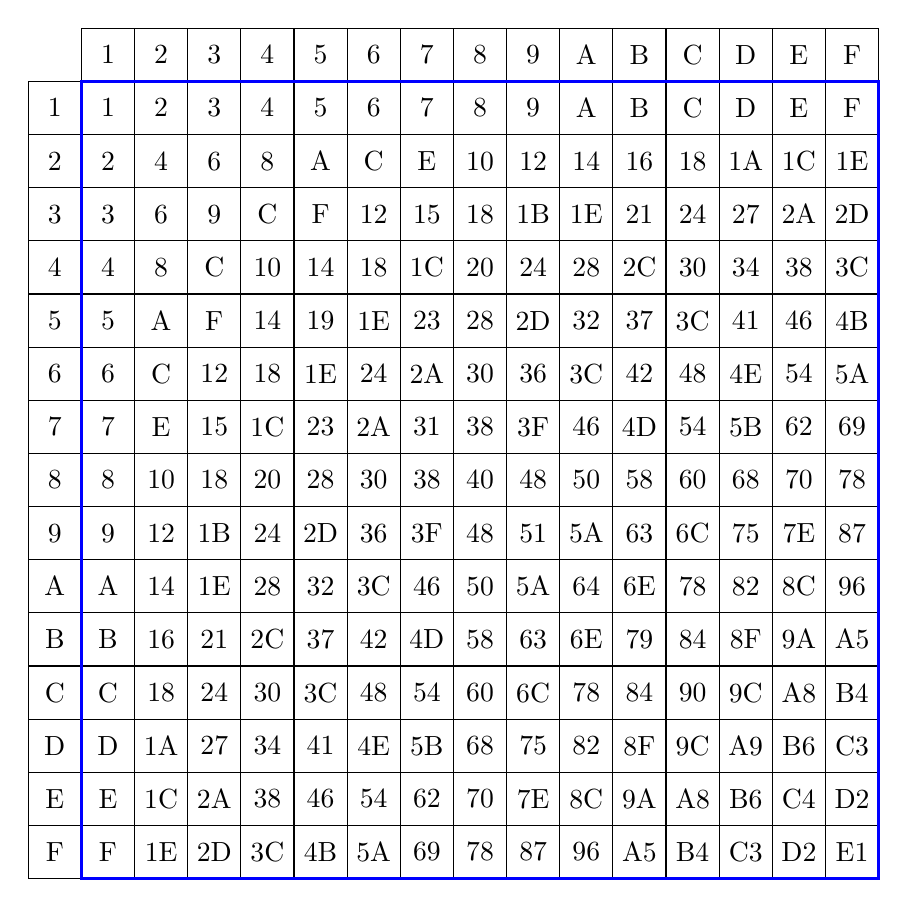
\begin{tikzpicture}[scale=0.675]
		% grid definition
		\draw (-1,0) grid (15,15);
		\draw (0,10) grid (15,16);
		\draw[line width=1pt, color=blue] (0,0) rectangle (15,15);
		
		% fill numbers
		\foreach \x in {1,2,3,...,15}
		\foreach \y in {1,2,3,...,15}
		\draw[shift={(-.5,-.5)}] (\x ,\y) node {\pgfmathHex{\number\numexpr\x*(16-\y)}\pgfmathresult\relax};
		
		% fill first row
		\foreach \x in {1,2,3,...,15}
		\draw[shift={(-.5,-.5)}] (\x , 16) node {\pgfmathHex{\x}\pgfmathresult};
		
		% fill first column
		\foreach \y in {1,2,3,...,15}
		\draw[shift={(-.5,-.5)}] (0, 16-\y) node {\pgfmathHex{\y}\pgfmathresult};
	\end{tikzpicture}
	\caption{Tavola Prodotti esadecimale}
	\label{tab:TavolaPitagoricaesadecimale}
\end{table}
\begin{table}[H]
	\centering
	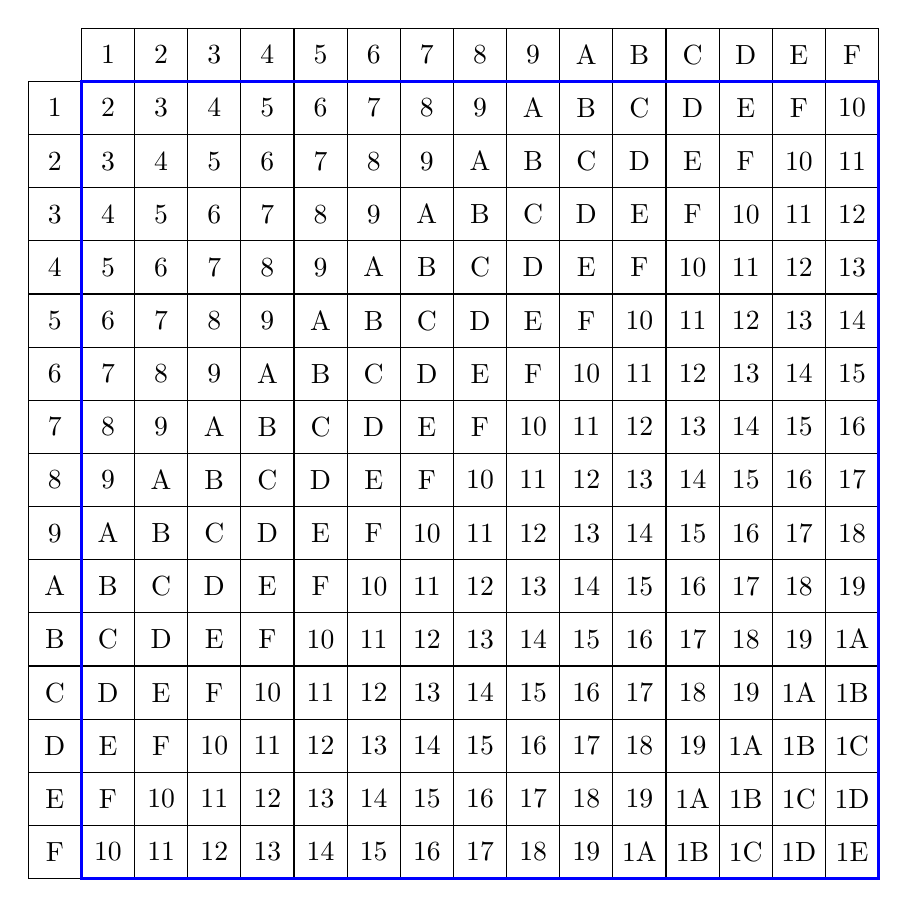
\begin{tikzpicture}[scale=0.675]
		% grid definition
		\draw (-1,0) grid (15,15);
		\draw (0,10) grid (15,16);
		\draw[line width=1pt, color=blue] (0,0) rectangle (15,15);
		
		% fill numbers
		\foreach \x in {1,2,3,...,15}
		\foreach \y in {1,2,3,...,15}
		\draw[shift={(-.5,-.5)}] (\x ,\y) node {\pgfmathHex{\number\numexpr\x+(16-\y)}\pgfmathresult\relax};
		
		% fill first row
		\foreach \x in {1,2,3,...,15}
		\draw[shift={(-.5,-.5)}] (\x , 16) node {\pgfmathHex{\x}\pgfmathresult};
		
		% fill first column
		\foreach \y in {1,2,3,...,15}
		\draw[shift={(-.5,-.5)}] (0, 16-\y) node {\pgfmathHex{\y}\pgfmathresult};
	\end{tikzpicture}
	\caption{Tavola somma esadecimale}
	\label{tab:Tavolaaddizioniesadecimale}
\end{table}
\subsection{Base otto}
\subsubsection{Conversioni}



\begin{table}[H]
	\centering
	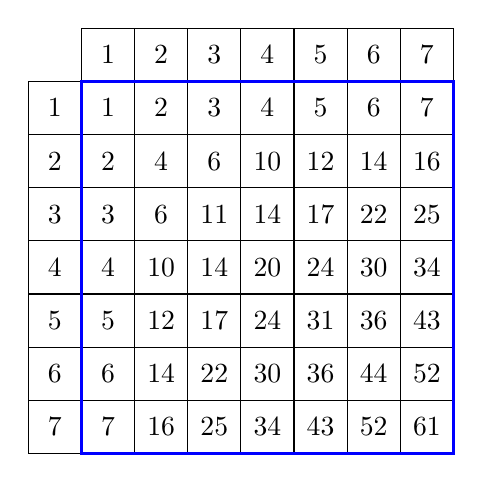
\begin{tikzpicture}[scale=0.675]
		% grid definition
		\draw (-1,0) grid (7,7);
		\draw (0,7) grid (7,8);
		\draw[line width=1pt, color=blue] (0,0) rectangle (7,7);
		
		% fill numbers
		\foreach \x in {1,2,3,...,7}
		\foreach \y in {1,2,3,...,7}
		\draw[shift={(-.5,-.5)}] (\x ,\y) node { \pgfmathoct{\number\numexpr\x*(8-\y)}\pgfmathresult\relax};
		
		% fill first row
		\foreach \x in {1,2,3,...,7}
		\draw[shift={(-.5,-.5)}] (\x , 8) node {\pgfmathoct{\x}\pgfmathresult};
		
		% fill first column
		\foreach \y in {1,2,3,...,7}
		\draw[shift={(-.5,-.5)}] (0, 8-\y) node {\pgfmathoct{\y}\pgfmathresult};
	\end{tikzpicture}
	\caption{Tavola Pitagorica ottale}
	\label{tab:TavolaPitagoricaottale}
\end{table}
\begin{table}[H]
	\centering
	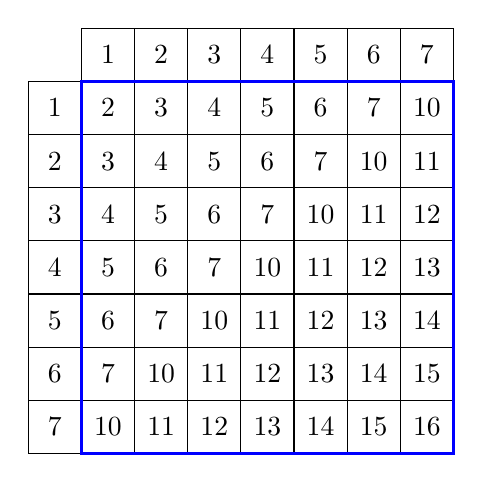
\begin{tikzpicture}[scale=0.675]
		% grid definition
		\draw (-1,0) grid (7,7);
		\draw (0,7) grid (7,8);
		\draw[line width=1pt, color=blue] (0,0) rectangle (7,7);
		
		% fill numbers
		\foreach \x in {1,2,3,...,7}
		\foreach \y in {1,2,3,...,7}
		\draw[shift={(-.5,-.5)}] (\x ,\y) node { \pgfmathoct{\number\numexpr\x+(8-\y)}\pgfmathresult\relax};
		
		% fill first row
		\foreach \x in {1,2,3,...,7}
		\draw[shift={(-.5,-.5)}] (\x , 8) node {\pgfmathoct{\x}\pgfmathresult};
		
		% fill first column
		\foreach \y in {1,2,3,...,7}
		\draw[shift={(-.5,-.5)}] (0, 8-\y) node {\pgfmathoct{\y}\pgfmathresult};
	\end{tikzpicture}
	\caption{Tavola Somma ottale}
	\label{tab:Tavolasommaottale}
\end{table}

	\chapter{Codifica Braille}
\label{Cha:CodificaBraille}
\begin{table}[H]
\begin{tabular}{cccc}
				\mytable{
					\braille{a} & a 1 \\
					\braille{b} & b 2 \\
					\braille{c} & c 3 \\
					\braille{d} & d 4 \\
					\braille{e} & e 5 \\
					\braille{f} & f 6 \\
					\braille{g} & g 7 \\
					\braille{h} & h 8 \\
					\braille{i} & i 9 \\
					\braille{j} & j 0 \\
					\braille{k} & k \\
					\braille{l} & l \\
					\braille{m} & m \\
					\braille{n} & n \\
					\braille{o} & o \\
				}&
				\mytable{
					\braille{p} & p \\
					\braille{q} & q \\
					\braille{r} & r \\
					\braille{s} & s \\
					\braille{t} & t \\
					\braille{u} & u \\
					\braille{v} & v \\
					\braille{w} & w \\
					\braille{x} & x \\
					\braille{y} & y \\
					\braille{z} & z \\
				}  &
				\mytable{
					\braille{{Capital}} & \{Maiuscolo\}\\
					\braille{{Upper}} & \{In alto\} \\
					%\braille{{Italic}} & \{Italic\} \\
				}
				&
				\mytable{
					\braille{{Number}} & \{Numero\} \\	
					\braille{{Letter}} & \{Lettera\} \\
				}   \\ 
				

			\end{tabular}
\caption[Codifica Braille]{ Codifica Braille (\copyright 1998-2010 William Park Licenza LPPL)}\label{tsd:}
\label{tab:CodificaBraille}
\end{table}
					
					
Ciao Mondo
					\braille{Ciao Mondo}
					
					1980
					\braille{{Number}1980}
	\input{extra/Cascii}
	\chapter{Algebra di Boole}
\label{cha:AlgebradiBoole}
%\FloatBarrier
\section{Variabili e funzioni booleane}
\label{sec:VariabiliBooleane}
Una variabile booleana\index{Variabile!booleana} è una variabile che può assumere solo due valori, che possono essere indicati o  con\nobs$0$\nobs e\nobs$1$ o con $basso$\nobs e\nobs$alto$, con $vero$\nobs o \nobs$falso$. Nella realtà, a questi valori sono  associati valori arbitrari es: $+5\si{\volt}$ $-5\si{\volt}$, $+12\si{\volt}$ $-12\si{\volt}$. 

 Un sistema si trova in un determinato stato a seconda del valore che assumono le variabili booleane associate.   Vi sono due variabili  particolari la variabile\nobs$0$ che assume solo il valore\nobs$0$ e la variabile \nobs$1$ che assume solo il valore\nobs$1$. 

Una funzione (operazione) booleana\index{Funzione!booleana} è una relazione  che ha in ingresso delle variabili indipendenti e in uscita una variabile dipendente.

A ogni sistema è associata una tabella detta tavola di verità\index{Tavola di verità}. Una tavola di verità rappresenta in forma tabellare, in base agli stati del sistema in entrata, lo stato del sistema in uscita. Si può facilmente provare %, utilizzando la tavola~\vref{tab:statisistema},  
che la tabella\vref{tab:totfunzzionilogiche} rappresenta tutte le funzioni logiche con due valori in entrata.

Due funzioni logiche sono equivalenti\index{Funzione!booleana!equivalente} se hanno la stessa tavola di verità. Esempio di questo sono la tabella\nobs\vref{tab:tabVeritaEOR} e la tabella\nobs\vref{tab:tabVeritaEOR2} che sono fra di loro equivalenti. 

Un metodo grafico per rappresentare una funzione logica  è il circuito che si ottiene combinando i simboli  elencati nella tabella\nobs\vref{tab:Portelogichetavver}. Un esempio di ciò sono  i due circuiti\nobs\vref{Tab:circuito2e3} che rappresentano entrambi la funzione $XOR$\index{Funzione!booleana!XOR}  ottenuta come combinazione di $AND$\index{Funzione!booleana!AND} e $OR$\index{Funzione!booleana!OR}

Principio di dualità: Se una funzione logica è vera, allora è vera la funzione che si ottiene scambiando $AND$ con  $OR$ e  $0$ con $1$ e viceversa.

\begin{table} %[H]
	%\centering
	\begin{tabular}{cccccccccccccccccc}
	\toprule
	A & B & $0$ & NOR & $\overline{A}$ &  &  & $\overline{B}$ & XOR & NAND & AND & XNOR &  & B & A &  & OR & $1$ \\ 
	\midrule
	1 & 1 & 0 & 0 & 0 & 0 & 0 & 0 & 0 & 0 & 1 & 1 & 1 & 1 & 1 & 1 & 1 & 1 \\ 
	1 & 0 & 0 & 0 & 0 & 0 & 1 & 1 & 1 & 1 & 0 & 0 & 0 & 0 & 1 & 1 & 1 & 1 \\ 
	0 & 1 & 0 & 0 & 1 & 1 & 0 & 0 & 1 & 1 & 0 & 0 & 1 & 1 & 0 & 0 & 1 & 1 \\ 
	0 & 0 & 0 & 1 & 1 & 0 & 0 & 1 & 0 & 1 & 0 & 1 & 1 & 0 & 0 & 1 & 0 & 1 \\ 
	\bottomrule
	\end{tabular}
	\caption{Funzioni logiche}
	\label{tab:totfunzzionilogiche}
\end{table}
\subsection{Esempi}
\label{sec:Esempiofunzlog}
Definire, utilizzando le funzioni logiche:

$tavolo=(legno,ferro,3gambe,4gambe,piano)$,

$auto=(3 porte,5 porte,ruote,motore)$, 

$penna=(sfera,stilografica,rossa,nera,verde,cancellabile,indelebile)$

Una cassaforte ha quattro lucchetti, x, y, v, w, che devono essere tutti aperti affinché la
cassaforte si apra.  Tre persone A, B, C,  hanno le  chiavi. A possiede le chiavi v e y; 
B ha le chiavi v e x e C tiene w e y. Le variabili A, B, C sono uguali a uno se la persona corrispondente è presente, altrimenti sono uguali a zero. Costruire la tavola
della verità della funzione $Y=f(A,B,C)$. La funzione  vale uno se e solo se la cassaforte può essere  aperta,
 esprimere f in forma algebrica. Per risolvere almeno la prima parte dell'esercizio costruiamo una tabella  che leghi le chiavi alle tre persone.
\begin{table}
	    \centering
		\begin{tabular}{c|cccc}
			& \textbf{x} & \textbf{y} &\textbf{v}& \textbf{w}\\
			\toprule 
			\textbf{A} &  & \textbullet &\textbullet & \\ 
			\textbf{B} & \textbullet &  & \textbullet& \\ 
			\textbf{C} &  & \textbullet & & \textbullet\\ 
			\bottomrule
		\end{tabular}
	\caption[]{Persone e chiavi}
	\label{tab:personeechiavi}
\end{table} 
Quindi: il sistema (la cassaforte aperta o chiusa), dipende da tre variabili $A$, $B$ e $C$ che assumono solo due valori $1$ se la chiave è presente o $0$ altrimenti. In uscita $Y$ può assumere due valori $1$ se la cassaforte è aperta o $0$ nell'altro caso. 

La tabella~\vref{tab:personeechiavi} permette di costruire la tavola di verità\nobs\vref{tab:tavolaveritacasaforte} della funzione. La tabella, dipendendo da tre variabili in ingresso, ha otto stati. Iniziamo a costruire la tavola di verità del sistema. Nella prima riga abbiamo che $A=0$, $B=0$ e $C=0$, poiché nessuna chiave è presente, la cassaforte rimane chiusa quindi $Y=0$. Nella seconda riga abbiamo che $A=0$, $B=0$ e $C=1$,  due chiavi sono presenti ma \nobs\vref{tab:personeechiavi} ci dice che queste non bastano e la cassaforte è chiusa e quindi $Y=0$. Il discorso è analogo  per le righe rimanenti. Nella riga quattro abbiamo che $A=0$, $B=1$ e $C=1$  sono presenti quattro chiavi e la cassaforte viene aperta per cui $Y=1$.  Stesso discorso la riga otto e anche in questo caso $Y=1$.
\begin{table}
		\centering
\begin{tabular}{c|c|c|c|c}
	& \textbf{A} & \textbf{B} & \textbf{C} & \textbf{Y} \\
	\toprule 
	1& 0 & 0 & 0 & 0 \\ 
	2& 0 & 0 & 1 &  0\\ 
	3& 0 & 1 & 0 &  0\\ 
	4& 0 & 1 & 1 &  1\\ 
	5& 1 & 0 & 0 &  0\\ 
	6& 1 & 0 & 1 &  0\\ 
	7& 1 & 1 & 0 &  0\\ 
	8& 1 & 1 & 1 &  1\\ 
	\bottomrule
\end{tabular} 
	\caption{Tavola di verità}
	\label{tab:tavolaveritacasaforte}
\end{table}
\section{Tavole di verità}
\label{sec:TavoleDiVeritA}
\begin{figure} %[H]
\centering
	\pagestyle{empty}
	% Set the overall layout of the tree
\tikzstyle{level 1}=[level distance=3.5cm, sibling distance=3.5cm]
\tikzstyle{level 2}=[level distance=3.5cm, sibling distance=2cm]
\tikzstyle{level 3}=[level distance=3cm, sibling distance=0.8cm] 
% Define styles for bags and leafs
%\tikzstyle{bag} = [text width=4em, text centered]
\tikzstyle{bag} =[shape=circle,draw,
text centered]
\begin{tikzpicture}[grow=right, sloped]
\matrix [row sep=1em] 
{
	\node[bag] {0}
	child{   
		node[bag] {0}
		child{
			node[bag] {0}
			child{
				node[bag]{0}
			}
			child{
				node[bag]{1}
			}
		}
		child {
			node[bag] {1}
			child{
				node[bag]{0}
			}
			child{
				node[bag]{1}
			}		
		}
	}
	child{
		node[bag]{1}
		child{
			node[bag] {0}
			child{
				node[bag]{0}
			}
			child{
				node[bag]{1}
			}
		}
		child {
			node[bag] {1}
			child{
				node[bag]{0}
			}
			child{
				node[bag]{1}
			}
		}   
	};
	&\\
	\draw (0,0) --  (10.5,0);
	\draw (0.0,1pt) -- (0.0,-3pt)
	node[anchor=north] {1};
	\draw (3.5,1pt) -- (3.5,-3pt)
	node[anchor=north] {2};
	\draw (7,1pt) -- (7,-3pt)
	node[anchor=north] {3};
	\draw (10,1pt) -- (10,-3pt)
	node[anchor=north] {4};\\
	\node[bag] {0}
	child{   
		node[bag] {0}
		child{
			node[bag] {0}
			child{
				node[bag]{0}
			}
			child{
				node[bag]{1}
			}
		}
		child {
			node[bag] {1}
			child{
				node[bag]{0}
			}
			child{
				node[bag]{1}
			}		
		}
	}
	child{
		node[bag]{1}
		child{
			node[bag] {0}
			child{
				node[bag]{0}
			}
			child{
				node[bag]{1}
			}
		}
		child {
			node[bag] {1}
			child{
				node[bag]{0}
			}
			child{
				node[bag]{1}
			}
		}   
	};\\
};
\end{tikzpicture}
	\caption{Stati del sistema}
	\label{tab:statisistema}
\end{figure}

Le funzioni logiche sono divise in gruppi. Il primo è formato dalle funzioni AND\index{Funzione!booleana!AND}, OR\index{Funzione!booleana!OR} e NOT\index{Funzione!booleana!NOT}. Segue il gruppo formato solo da NAND\index{Funzione!booleana!NAND}. Infine quello composto solo  da NOR\index{Funzione!booleana!NOR}. Ogni gruppo è tale perché in grado di generare le rimanenti funzioni. La figura~\vref{tab:Portelogichetavver} riporta le tavole di verità di queste funzioni. 

Combinando fra di loro le funzioni  otteniamo altre funzioni come viene per esempio, nella tabella~\vref{tab:ComposizionePorte}. 

La tabella~\vref{tab:statisistema} da in verticale di quante righe deve avere una tavola di verità.  Con una variabile due righe,  due variabili  otteniamo quattro righe etc. Mentre in orizzontale,in base al numero delle variabili, percorrendo i grafi da sinistra verso destra, avremo tutti i possibili stati di un sistema.
\subsection{Funzione AND}
\label{sub:funzioneAND}
La funzione AND\index{Funzione!booleana!AND} ha due valori in entrata ed  un valore in uscita che è vero solo quando sono veri entrambi i valori in entrata. Il simbolo che la rappresenta l'operazione è il prodotto.

Nella realtà casi in cui si usano funzioni AND sono molteplici. In genere si usa una funzione AND\index{Funzione!booleana!AND} quando  si eseguono due azioni in contemporaneamente come per esempio nel dispositivi di azionamento di una pressa in cui si premono contemporaneamente due pulsanti in modo da impegnare entrambe le mani, evitando così incidenti. 

Un esempio della funzione AND\index{Funzione!booleana!AND} è il seguente circuito\nobs\vref{tab:elettricoAND}. Abbiamo un circuito con due pulsanti in serie.  La lampada si accende solo premendo solo contemporaneamente i due interruttori.
\begin{table}[H]
	\centering
	\begin{circuitikz} \draw
		(0,0)--(0,2)
		(5,0)--(5,2)
		(0,0) to[lamp] (2,0)
		(2,0) to[battery] (5,0)
		(0,2) to[opening switch] (3,2)
		(3,2) to[opening switch] (5,2);
	\end{circuitikz}
	\caption{Circuito AND}
	\label{tab:elettricoAND}
\end{table}
	
La tabella\nobs\ref{tab:Portelogichetavver} mostra la tavola di verità\index{Tavola di verità!AND} della $AND$\index{Funzione!booleana!AND} e il simbolo grafico associato.
\subsection{Funzione OR}
\label{sub:funzioneOR}
La funzione OR\index{Funzione!booleana!OR} ha due valori in entrata e un valore in uscita. Questo valore è vero quando almeno uno dei valori in ingresso è vero. Il simbolo che la rappresenta è la somma. 

Un esempio dell'uso della funzione OR\index{Funzione!booleana!OR} è l'impianto di illuminazione di una stanza in cui due interruttori distinti permettono di accendere una lampadina.

Un circuito in parallelo, come il circuito\nobs\vref{tab:ZunzioneOR}, rappresenta la funzione OR\index{Funzione!booleana!OR}. Per accendere la lampadina basta premere almeno un interruttore.
\begin{table}
	\centering
	\begin{circuitikz} \draw
		(0,0)--(0,2)
		(5,0)--(5,2)
		(0,0) to[lamp] (2,0)
		(2,0) to[battery] (5,0)
		(0,2)--(1,2)
		(1,1)--(1,3)
		(4,1)--(4,3)
		(4,2)--(5,2)
		(1,3) to[opening switch] (4,3)
		(1,1) to[opening switch] (4,1);
	\end{circuitikz}
	\caption{Circuito OR}
	\label{tab:ZunzioneOR}
\end{table}
La tabella\nobs\ref{tab:Portelogichetavver} mostra la tavola di verità\index{Tavola di verità!OR} della OR\index{Funzione!booleana!OR} e il simbolo grafico associato.
\subsection{Funzione NOT}
\label{sub:funzionenot}
La funzione NOT ha un solo valore in entrata e un solo valore in uscita. Il valore in uscita è l'opposto a quello in ingresso. Il simbolo che rappresenta l'operazione è un trattino che si pone sopra la variabile.

Un esempio dell'uso della funzione NOT\index{Funzione!booleana!NOT} è per esempio l'interruttore della luce di cortesia di un'auto che si accende aprendo la portiera.

Un circuito come il circuito\nobs\vref{tab:CircuitoNOT} rappresenta la funzione NOT. La tabella\nobs\ref{tab:Portelogichetavver} mostra la tavola di verità\index{Tavola di verità!NOT} della NOT e il simbolo grafico associato.
\begin{table}
	\centering
	 \begin{circuitikz} \draw
		(0,0)--(0,2)
		(6,0)--(6,2)
		(0,1) to[lamp] (6,1)
		(0,2)--(3,2)
		(3,2) to[battery,v_<=$+-$] (6,2)
		(0,0) to[opening switch] (3,0)
		(3,0) to[battery,v_<=$+-$] (6,0);
	\end{circuitikz}
	\caption{Circuito NOT}
	\label{tab:CircuitoNOT}
\end{table}
	
\subsection{Funzione XOR}
\label{sub:funzioneXOR}
La funzione XOR\index{Funzione!booleana!XOR} ha due valori in entrata ed un valore in uscita che è vero quando solo uno dei valori in ingresso è vero.

Il circuito\nobs\vref{tab:circuitoXOR} rappresenta un OR esclusivo. Sono due gruppi di pulsanti in parallelo messe in serie. La seconda serie di pulsanti sono i negati dei precedenti. Quando vien premuto il primo pulsante $A$ il pulsante $\overline{A}$ del secondo circuito viene aperto e viceversa, analogamente per il pulsante $B$. In questo circuito la corrente passa e  lampadina si accende, solo se è premuto un solo pulsante ma non entrambi.

La tabella\nobs\ref{tab:Portelogichetavver} mostra la tavola di verità della XOR\index{Tavola di verità!XOR} e il simbolo grafico associato.
\begin{table} %[H]
		\centering
		\begin{circuitikz} \draw
			(0,0)--(0,2)
			(7,0)--(7,2)
			(0,0) to[lamp] (3,0)
			(3,0) to[battery] (7,0)
			(0,2)--(1,2)
			(1,1)--(1,3)
			(3,1)--(3,3)
			(3,2)--(4,2)
			(4,1)--(4,3)
			(6,1)--(6,3)
			(6,2)--(7,2)
			(1,3) to[opening switch=$A$] (3,3)
			(1,1) to[opening switch=$B$] (3,1)
			(4,1) to[closing switch=$\overline{B}$] (6,1)
			(4,3) to[closing switch=$\overline{A}$] (6,3);
		\end{circuitikz}
	\caption{Circuito XOR}
	\label{tab:circuitoXOR}
	\end{table}
\subsection{Funzione NAND}
\label{sub:funzioneNAND}
La funzione NAND\index{Funzione!booleana!NAND} ha due valori in entrata ed ha un valore in uscita che è falso solo quando sono veri entrambi i valori in entrata.

La tabella\nobs\ref{tab:Portelogichetavver} mostra la tavola di verità\index{Tavola di verità!NAND} della $NAND$\index{Funzione!booleana!NAND} e il simbolo grafico associato. La $NAND$ è la negazione di $AND$\index{Funzione!booleana!AND}.

\subsection{Funzione NOR}
\label{sub:funzioneNOR}
La funzione NOR\index{Funzione!booleana!NOR} ha due valori in entrata ed ha un valore in uscita che è vero solo quando sono falsi entrambi i valori in entrata.

La tabella\nobs\ref{tab:Portelogichetavver} mostra la tavola di verità\index{Tavola di verità!NOR} della NOR\index{Funzione!booleana!NOR} e il simbolo grafico associato. La NOR è la negazione di OR 
\subsection{Funzione XNOR}
\label{sub:funzioneXNOR}
La funzione XNOR\index{Funzione!booleana!XNOR} ha due valori in entrata ed ha un valore in uscita che è vero solo quando sono falsi entrambi i valori in entrata o quando sono entrambi veri. 

La tabella\nobs\ref{tab:Portelogichetavver} mostra la tavola di verità\index{Tavola di verità!XNOR} della XNOR e il simbolo grafico associato. La XNOR è la negazione di XOR 

Il circuito\nobs\vref{tab:circuitoXNOR} è formato da due blocchi di pulsanti in serie messi in parallelo. Quando vien premuto il primo pulsante $A$ il pulsante $\overline{A}$ del secondo circuito viene aperto e viceversa, analogamente per il pulsante $B$. La lampadina si accende o quando entrambi i pulsanti $A$ e $B$ sono premuti o entrambi i  pulsanti $A$ e $B$ sono tenuti alzati.
\begin{table}[H]
	\centering
	\begin{circuitikz} \draw
		(0,0)--(0,2)
		(7,0)--(7,2)
		(0,0) to[lamp] (3,0)
		(3,0) to[battery] (7,0)
		(0,2)--(1,2)
		(1,1)--(1,3)
		(6,1)--(6,3)
		(6,2)--(7,2)
		(1,3) to[opening switch=$A$] (4,3)
		(4,3) to[opening switch=$B$] (6,3)
		(1,1) to[closing switch=$\overline{A}$] (4,1)
		(4,1) to[closing switch=$\overline{B}$] (6,1);
	\end{circuitikz}
	\caption{Circuito XNOR}
	\label{tab:circuitoXNOR}
\end{table}
Come si è detto a una funzione logica è possibile associare una tavola di verità\index{Tavola di verità!Costruire}. Un esempio di costruzione  è la tabella~\vref{tab:tabVeritaEOR}. Il metodo usato è molto semplice,  prevede di suddividere la funzione nelle sue componenti e risolverle partendo da sinistra verso destra. Questo deve essere fatto rispettando le convenzioni di precedenza, cioè le negazioni (funzione NOT), poi i prodotti (Funzione AND\index{Funzione!booleana!AND}), e infine le somme (Funzione OR\index{Funzione!booleana!OR}).Possiamo cambiare le  precedenze mettendo fra  delle parentesi le operazioni che devono essere eseguite prima.
In conclusione, abbiamo parlato di tavola di verità\index{Tavola di verità}, circuito, funzione logica, che sono concetti fra loro equivalenti\vref{tab:FunzioneTavolaCircuito} e fra loro connessi.
\begin{table} 
	\centering
	\begin{tikzpicture}[very thick,node distance=5cm,text centered,minimum size=3cm]
		\node [circle, draw] (a) {Funzione logica};
		\node [circle, draw] (b) [above right=of a] {Tavola di verità};
		\node [circle, draw] (c) [above left=of a]{Circuito};
		\draw [<->] (a) to (b);
		\draw [<->] (b) to (c);
		\draw [<->] (c) to (a);
	\end{tikzpicture}
	\caption{Funzione, Tavola e Circuito}
	\label{tab:FunzioneTavolaCircuito}
\end{table}
\begin{table}
	\centering
	\begin{tabular}{@{}cc@{\hspace{2cm}}cc@{}}
	\begin{truthtable}{AND}
	\toprule
	$A$&$B$&$AB$\\
	\midrule           
	0&0&0\\
	1&0&0\\
	0&1&0\\
	1&1&1\\
	\bottomrule
	\end{truthtable}
	& \cport{and} &
	\begin{truthtable}{NAND}
	\toprule
	$A$&$B$&$A\mathbin{\overline{\wedge}}B$\\
	\midrule
	0&0&1\\
	1&0&1\\
	0&1&1\\
	1&1&0\\
	\bottomrule
	\end{truthtable}
	& \cport{nand} \\
	\addlinespace[3ex]
	\begin{truthtable}{OR}
	\toprule
	$A$&$B$&$A+B$\\
	\midrule         
	0&0&0\\
	1&0&1\\
	0&1&1\\
	1&1&1\\
	\bottomrule
	\end{truthtable}
	& \cport{or} &
	\begin{truthtable}{NOR}
	\toprule
	$A$&$B$&$A\mathbin{\overline{\vee}}B$\\
	\midrule
	0&0&1\\
	1&0&0\\
	0&1&0\\
	1&1&0\\
	\bottomrule
	\end{truthtable}
	& \cport{nor} \\
	\addlinespace[3ex]
	\begin{truthtable}{XOR}
	\toprule
	$A$&$B$&$A\XOR B$\\
	\midrule         
	0&0&0\\
	1&0&1\\
	0&1&1\\
	1&1&0\\
	\bottomrule
	\end{truthtable}
	& \cport{xor} &
	\begin{truthtable}{XNOR}
	\toprule
	$A$&$B$&$A\mathbin{\overline{\XOR}}B$\\
	\midrule
	0&0&1\\
	1&0&0\\
	0&1&0\\
	1&1&1\\
	\bottomrule
	\end{truthtable}
	& \cport{xnor} \\
	\addlinespace[3ex]
	\multicolumn{4}{c}{%
		\begin{tabular}{@{}cc@{}}
		\begin{truthtable}[2]{NOT}
		\toprule
		$A$&$\overline{A}$\\
		\midrule         
		0&1\\
		1&0\\
		\bottomrule
		\end{truthtable}
		& \cport{not}
		\end{tabular}}
	\end{tabular}
	\caption{Porte logiche}
	\label{tab:Portelogichetavver}
\end{table} 
\begin{table} %[H]
	\centering
	\begin{tabular}{ccc}
	\toprule
	\begin{circuitikz} \draw
	(0,0) node[and port] (myand) {}
	(1,0) node[not port] (mynot) {}
	(myand.out) -- (mynot.in)
	;\end{circuitikz}&&\begin{circuitikz} \draw
	(0,0) node[nor port]  {}
	;\end{circuitikz} \\
	AND +  NOT &=&NAND \\
	\midrule
	\begin{circuitikz} \draw
	(0,0) node[or port] (myor) {}
	(1,0) node[not port] (mynot) {}
	(myor.out) -- (mynot.in)
	;\end{circuitikz}&& \begin{circuitikz} \draw
	(0,0) node[nor port]  {}
	;\end{circuitikz} \\
	OR +  NOT &=&NOR  \\ 
	\midrule
	\begin{circuitikz} \draw
	(0,0) node[xor port] (myxor) {}
	(1,0) node[not port] (mynot) {}
	(myxor.out) -- (mynot.in)
	;\end{circuitikz}&& \begin{circuitikz} \draw
	(0,0) node[xnor port]  {}
	;\end{circuitikz} \\
	XOR +  NOT &=&XNOR  \\ 
	\bottomrule
	\end{tabular} 
	\caption{Composizione porte}%
	\label{tab:ComposizionePorte}%
\end{table}
\section{Proprietà dell'algebra algebra booleana}
\label{sec:Algebrabooleana}
La tabella\nobs\vref{Tab:AlgebrAbOOLEAN} elenca le principali proprietà delle funzioni AND\index{Funzione!booleana!AND} e OR\index{Funzione!booleana!OR} e mostra come le proprietà delle funzioni siano legate tramite il principio di dualità. Infatti, osservando la tabella si vede come le proprietà elencate a sinistra trovino il loro corrispondente duale a destra e viceversa. La tabella\nobs\vref{Tab:funzlogSemp} mostra come ottenere i risultati. Non vengono dimostrate tutte le relazioni inquarto le altre si ottengono per dualità.

%\altapriorita{Specificare meglio}
Una funzione logica non è unica ma può essere scritta in modi fra di loro equivalenti. La tabella\nobs\vref{Tab:funzlogSemp} mostra come con pochi passaggi si può passare da una funzione logica a una equivalente.
\begin{table}%[H]
\centering
\begin{tabular}{lcl}
\toprule
&PROPRIET\'A&\\
&$\overline{\overline{A}}=A$&\\
$A+0=A$&Elemento neutro&$A\cdot1=A$\\
$A+1=1$&Assorbimento&$A\cdot0=0$\\
$A+A=A$&Idempotenza&$A\cdot A=A$\\
$A+\overline{A}=1$&&$A\cdot\overline{A}=0$\\
$A+B=B+A$&Commutativa&$A\cdot B=B\cdot A$\\
$(A\cdot B)\cdot C=A\cdot(B\cdot C)=A\cdot B\cdot C$&Associativa&$(A+B)+C=A+(B+C)=A+B+C$\\
\midrule
&TEOREMI&\\
\midrule
$A+A\cdot B=A$&&$A\cdot(A+B)=A$\\
$A+\overline{A}\cdot B=A+B$&&$A\cdot (\overline{A}+B)=AB$\\
$(A+B)\cdot(A+C)=A+B\cdot C$&&$A\cdot B+A\cdot C=A\cdot(B+C)$\\
$(A+B)\cdot(\overline{A}+C)=\overline{A}\cdot B+A\cdot C$&&$A\cdot B+\overline{A}\cdot C=(\overline{A}+B)\cdot(A+B)$\\
\midrule
&TEOREMI DI DE MORGAN&\\
\midrule
$\overline{A+B}=\overline{A}\cdot\overline{B}$&&$\overline{A\cdot B}=\overline{A}+\overline{B}$\\
\bottomrule
\end{tabular}
\caption{Teoremi e proprietà algebra di Boole}%
\label{Tab:AlgebrAbOOLEAN}%
\end{table}
\begin{table}
\centering
\begin{tabular}{lcl}
\toprule
%\midrule
PROPRIET\'A&&DIMOSTRAZIONE\\
\midrule
$A+A\cdot B=A$&&$A+A\cdot B=$\\
&&$=A\cdot(1+B)=$\\
&&$=A\cdot1=A$\\ 
\midrule
$A+\overline{A}\cdot B=A+B$&&$A+A\cdot B+\overline{A}\cdot B=$\\
&&$=A+(A+\overline{A})\cdot B=$\\
&&$=A+1\cdot B=$\\
&&$=A+B$\\
\midrule
$(A+B)\cdot(A+C)=A+B\cdot C$&&$(A+B)\cdot(A+C)=$\\
&&$A\cdot A+A\cdot C+A\cdot B+B\cdot C=$\\
&&$=A+A\cdot C+A\cdot B+B\cdot C=$\\
&&$=A\cdot(1+C) +A\cdot B+B\cdot C=$\\
&&$=A\cdot 1 +A\cdot B+B\cdot C=$\\
&&$=A\cdot(1+B)+B\cdot C=$\\
&&$A+B\cdot C$\\
\midrule
$(A+B)\cdot(\overline{A}+C)=\overline{A}\cdot B+A\cdot C$&&$(A+B)\cdot(\overline{A}+C)$\\
&&$\overline{A}\cdot A+ A\cdot C +\overline{A}\cdot B+B\cdot A\cdot C$\\
&&$A\cdot B+\overline{A}\cdot B+B\cdot C$\\
&&$(A+B)\cdot C+\overline{A}\cdot B$\\
&&$(A+\overline{A}\cdot B)\cdot C+\overline{A}\cdot B$\\
&&$A\cdot C+\overline{A}\cdot B\cdot C+\overline{A}\cdot B$\\
&&$A\cdot C+\overline{A}\cdot B(C+1)$\\
&&$A\cdot C+\overline{A}\cdot B$\\
\bottomrule
\end{tabular}
\caption{Semplificazioni}
\label{Tab:funzlogSemp}
\end{table}
\section{Trovare la tavola di verità di una funzione}
\label{sec:Trovaretavolaveritàfunzione}
Per trovare data una funzione, la tavola di verità\index{Tavola di verità}, basta sostituire alle variabili booleane  i valori in ingresso e vedere cosa ha la funzione in uscita. 

Consideriamo la funzione $Y=A\cdot\overline{B}+\overline{A}\cdot B$  possiamo costruire la tabella\nobs\vref{tab:tabVeritaEOR} che fornisce tutti i calcoli necessari. Si procede sostituendo alle variabili tutti i valori possibili e ottenendo dopo i calcoli i risultati della colonna sette 

Analogo ragionamento è per $Y=(A+B)\cdot(\overline{A}+\overline{B})$ e ottenere la tabella\nobs\vref{tab:tabVeritaEOR2}.

Per $Y=\overline{A}\cdot\overline{B}\cdot C+\overline{A}\cdot B\cdot\overline{C}+\overline{A}\cdot B\cdot C+A\cdot B\cdot C$ otteniamo la tavola di verità\nobs\vref{Tab:esempio2bool}\index{Tavola di verità}

La tavola di verità per $Y=\overline{A}\cdot (A+B)+\overline{C}+B\cdot C$ e per $Y=B+\overline{C}$ è\nobs\vref{Tab:Tabveres1}
\begin{table}
	\centering
	\begin{tabular}{ccccccccccc}
		\toprule
		\multicolumn{10}{c}{$A\cdot\overline{B}+\overline{A}\cdot B$} \\ 
		&  &  & 1 & 3 & 2 & 7 & 4 & 6 & 5 \\ 
		A & B &  & $A$&$\cdot$  &$\overline{B}$&$+$& $\overline{A}$ &$\cdot$ &$B$  \\ 
		\cmidrule{1-2}\cmidrule{4-10}
		1 & 1 &  & 1 & 0 & 0 & 0 & 0 & 0 & 1 \\ 
		1 & 0 &  & 1 & 1 & 1 & 1 & 0 & 0 & 0 \\ 
		0 & 1 &  & 0 & 0 & 0 & 1 & 1 & 1 & 1 \\ 
		0 & 0 &  & 0 & 0 & 1 & 0 & 1 & 0 & 0 \\ 
		\bottomrule
	\end{tabular}
	\caption[]{Tavola di verità di $A\cdot\overline{B}+\overline{A}\cdot B$}
	\label{tab:tabVeritaEOR}
\end{table}
\begin{table}
	\centering
	\begin{tabular}{ccccccccccc}
		\toprule
		\multicolumn{10}{c}{$(A+B)\cdot(\overline{A}+\overline{B})$} \\ 
		&  &  & 1 & 3 & 2 & 7 & 4 & 6 & 5 \\ 
		A & B &  & $(A$&$+$  &$B)$ &$\cdot$ &$(\overline{A}$&$+$&$\overline{B})$  \\ 
		\cmidrule{1-2}\cmidrule{4-10}
		1 & 1 &  & 1 & 1 & 1 & 0 & 0 & 0 & 0 \\ 
		1 & 0 &  & 1 & 1 & 0 & 1 & 0 & 1 & 1 \\ 
		0 & 1 &  & 0 & 1 & 1 & 1 & 1 & 1 & 0 \\ 
		0 & 0 &  & 0 & 0 & 0 & 0 & 1 & 1 & 1 \\ 
		\bottomrule
	\end{tabular}
	\caption[]{Tavola di verità di $(A+B)\cdot(\overline{A}+\overline{B})$}
	\label{tab:tabVeritaEOR2}
\end{table}
\section{Trovare la funzione data la tavola di verità}
\label{sec:Trovarefunzionedatatavolaverità}
Per trovare la funzione, nota la tavola di verità\index{Tavola di verità!trovare!funzione}, possiamo utilizzare due metodi\footnote{I due metodi sono duali come si nota leggendo di seguito} 
\subsection{Somma di prodotti canonici} 
Per trovare data la tavola di verità la funzione si usa il metodo della somma di prodotti canonici\index{Somma prodotti canonici!\see{Mintermini}}. Ogni funzione logica si può scrivere come somma di prodotti detti mintermini\index{Mintermini}. Questi prodotti sono costituiti da prodotti di tutte le variabili in forma diretta o negata. Ogni mintermine assume il valore logico 1.

Nell'esempio uno si inizia dalla tavola\nobs\vref{Tab:esempio2bool},  si individuano le righe che hanno come risultato uno e si costruisce la somma dei mintermini. Nella riga due della tavola di verità si ha come risultato uno. Dato che le variabili $A$ $B$ assumono valore zero nel prodotto si inserisce il loro complemento e otteniamo $\overline{A}\cdot \overline{B}\cdot C$.

Si continua con lo stesso criterio ed otteniamo\[Y=2+3+4+8=\overline{A}\cdot\overline{B}\cdot C+\overline{A}\cdot B\cdot\overline{C}+\overline{A}\cdot B\cdot C+A\cdot B\cdot C\] cioè la funzione associata.
\begin{table}
	\centering
	\begin{tabular}{lccc|c}
		&A&B&C&Y\\
		\toprule
		1&0&0&0&0\\
		2&0&0&1&\textbf{1}\\
		3&0&1&0&\textbf{1}\\
		4&0&1&1&\textbf{1}\\
		5&1&0&0&0\\
		6&1&0&1&0\\
		7&1&1&0&0\\
		8&1&1&1&\textbf{1}\\
	\end{tabular}
	\caption[]{Tabella verità di $Y=\overline{A}\cdot\overline{B}\cdot C+\overline{A}\cdot B\cdot\overline{C}+\overline{A}\cdot B\cdot C+A\cdot B\cdot C$}
	\label{Tab:esempio2bool}
\end{table}
%\begin{table}
%	\begin{equation}
%	Y=2+3+4+8=\overline{A}\overline{B}C+\overline{A}B\overline{C}+\overline{A}BC+ABC
%	\end{equation}
%	\caption[]{Funzione booleana esempio 1}
%	\label{tab:esempio2funbool}
%\end{table}
\subsection{Prodotto di somme canoniche}
Per trovare, data la tavola di verità\index{Tavola di verità!trovare!funzione}, la funzione si usa il metodo della prodotti di somme  canoniche\index{Prodotti somme canoniche|see{Maxtermini} }. Ogni funzione logica si può scrivere come prodotto di somme detti maxtermini\index{Maxtermini}. Questi prodotti sono costituiti da somme di tutte le variabili in forma diretta o negata. Ogni maxtermine assume il valore logico 0.
Nell'esempio 1 si inizia dalla tavola\nobs\vref{Tab:esempio2bool}  si individuano le righe che hanno come risultato zero e si costruisce il prodotto dei maxtermini. Nella riga uno della tavola di verità si ha come risultato zero. Dato che le variabili $A$ $B$ $C$ assumono valore zero il max termine sarà $(A+B+C)$ 

Si continua con lo stesso criterio ed otteniamo\[Y=1+5+6+7=(A+B+C)(\overline{A}+B+C)(\overline{A}+B+ \overline{C})(\overline{A}+\overline{B}+C) \]
\section{Trovare il circuito corrispondente}
\label{Trovarecircuito}
\'E relativamente facile disegnare uno schema grafico che rappresenti un circuito. Partendo da \[Y=\overline{A}\cdot\overline{B}\cdot C+\overline{A}\cdot B\cdot\overline{C}+\overline{A}\cdot B\cdot C+A\cdot B\cdot C\] otteniamo\nobs\vref{tab:circuito1}. Il disegno è ottenuto ricordando le precedenza nelle operazioni per cui prima la negazione poi il prodotto e infine la somma.

I circuiti corrispondenti a \[(A+B)\cdot(\overline{A}+\overline{B})=A\cdot\overline{B}+\overline{A}\cdot B\] sono\nobs\vref{Tab:circuito2e3}
 In questo caso gli OR\index{Funzione!booleana!OR} hanno la precedenza perché contenuti in parentesi.
	
I circuiti corrispondenti a \[A\cdot B+\overline{A}\cdot\overline{B}=(\overline{A}+ B)\cdot(A+\overline{B})\] sono i circuiti disegnati in\nobs\vref{tab:circuito4e5}

Il circuito corrispondente a \[Y=\overline{A}\cdot (A+B)+\overline{C}+B\cdot C\] è il circuito disegnato in\nobs\vref{tab:circuito6}

Il circuito corrispondente a \[Y=\overline{A}\cdot C+\overline{A}\cdot B+B\cdot C\] è il circuito disegnato in\nobs\vref{tab:circuito7}
\begin{table}
\tikzstyle{branch}=[fill,shape=circle,minimum size=3pt,inner sep=0pt]
\centering
\begin{tikzpicture}
\node (A) at (0,0) {A};
\node (B) at (1,0) {B};
\node (C) at (2,0) {C};
\node[not gate US, draw] at ($(A)+(3,-2)$) (Not1) {};
\node[not gate US, draw] at ($(B)+(2,-1)$) (Not2) {};
\node[not gate US, draw] at ($(B)+(2,-2.5)$) (Not3) {};
\node[not gate US, draw] at ($(B)+(2,-3.4)$) (Not4) {};
\node[not gate US, draw] at ($(B)+(2,-3.9)$) (Not5) {};
\node[and gate US, draw, logic gate inputs=nnn, anchor=input 2] at ($(Not1.output-|Not2.output)+(1,.5)$) (and1){}; 
\node[and gate US, draw, logic gate inputs=nnn, anchor=input 3] at ($(Not3.output-|Not4.output)+(1,-.65)$) (and2){}; 
\node[and gate US, draw, logic gate inputs=nnn, anchor=input 3] at ($(Not5.output)+(1,-.4)$) (and3){}; 
\node[and gate US, draw, logic gate inputs=nnn, anchor=input 3] at ($(and3)+(-.4,-1.1)$) (and4){}; 
\node[or gate US, draw, logic gate inputs=nnnn, anchor=input 2] at ($(and2)+(3,-.5)$) (or1){};  
\draw (B)|-node[branch] {}(Not1.input);
\draw (A)|-node[branch] {}(Not2.input);
\draw(C)|-node[branch] {}(and1);
\draw(Not1.output)--([xshift=0.3cm]Not1.output) |-(and1.input 3);
\draw(Not2.output)--([xshift=0.3cm]Not2.output) |-(and1.input 1);
\draw (C)|-node[branch] {}(Not3.input);
\draw (A)|-node[branch] {}(Not4.input);
\draw(Not3.output)--([xshift=0.3cm]Not3.output) |-(and2.input 1);
\draw(Not4.output)--([xshift=0.3cm]Not4.output) |-(and2.input 3);
\draw(B)|-node[branch] {}(and2);
%
\draw(A)|-node[branch] {}(Not5.input);
\draw(Not5.output)--([xshift=0.3cm]Not5.output) |-(and3.input 1);
\draw(B)|-node[branch] {} (and3.input 2);
\draw(C)|-node[branch] {} (and3.input 3);
%
\draw(A)|-node[branch] {}(and4.input 1);
\draw(B)|- node[branch] {}(and4.input 2);
\draw(C)|- node[branch] {}(and4.input 3);
\draw(and1.output)--  ([xshift=0.5cm]and1.output) |- (or1.input 1);
\draw(and2.output)--([xshift=0.3cm]and2.output) |- (or1.input 2);
\draw(and3.output)--([xshift=0.3cm]and3.output) |- (or1.input 3);
\draw(and4.output)--  ([xshift=0.5cm]and4.output) |- (or1.input 4);
\draw (or1.output) -- ([xshift=0.5cm]or1.output) node[above] {};
\end{tikzpicture}
	\caption[]{Circuito corrispondente a $Y=\overline{A}\cdot\overline{B}\cdot C+\overline{A}\cdot B\cdot\overline{C}+\overline{A}\cdot B\cdot C+A\cdot B\cdot C$}
	\label{tab:circuito1}
\end{table}
\begin{table}
	%\centering
	\begin{circuitikz} \draw
		(0,0)--(0,4)
		(1,0)--(1,4)
		(0,0) node[anchor=east] {A}
		(1,0) node[anchor=east] {B}
		(5,3.0) node[or port] (myor1) {}
		
		(0,3.3)to[short, *-] (myor1.in 1)
		(1,2.7)to[short, *-](myor1.in 2)
		(2,1.8) node[not port] (mynot1) {}
		(0,1.8)to[short, *-](mynot1.in)
		(2,0.3) node[not port] (mynot2) {}
		(1,0.3)to[short, *-](mynot2.in)
		(5,1.1) node[or port] (myor2) {}
		(mynot1.out)-|(myor2.in 1)
		(mynot2.out)-|(myor2.in 2)
		(7.0,2.0) node[and port] (myand1) {}
		(myor1.out)-|(myand1.in 1)
		(myor2.out)-|(myand1.in 2);
	\end{circuitikz}
	\begin{circuitikz} \draw
		(0,0)--(0,4)
		(1,0)--(1,4)
		(0,0) node[anchor=east] {A}
		(1,0) node[anchor=east] {B}
		(5,3.0) node[and port] (myand1) {}
		(2,3.3) node[not port] (mynot1) {}
		(5,1.1) node[and port] (myand2) {}
		(2,0.8) node[not port] (mynot2) {}
		(7.0,2.0) node[or port] (myor1) {}	
		(0,3.3)to[short, *-] (mynot1.in)
		(mynot1.out)--(myand1.in 1)
		(1,2.7)to[short, *-](myand1.in 2)
		(0,3.3)to[short, *-](mynot1.in)
		(1,0.8)to[short, *-](mynot2.in)
		(0,1.4)to[short, *-](myand2.in 1)
		(mynot2.out)--(myand2.in 2)
		(myand1.out)-|(myor1.in 1)
		(myand2.out)-|(myor1.in 2);
	\end{circuitikz}
	\caption[]{Circuiti corrispondenti a $(A+B)\cdot(\overline{A}+\overline{B})=A\cdot\overline{B}+\overline{A}\cdot B$}
	\label{Tab:circuito2e3}
\end{table}
\begin{table} %[H]
	\begin{circuitikz} \draw
		(0,0)--(0,4)
		(1,0)--(1,4)
		(0,0) node[anchor=east] {A}
		(1,0) node[anchor=east] {B}
		(5,3.0) node[and port] (myand1) {}
		
		(0,3.3)to[short, *-] (myand1.in 1)
		(1,2.7)to[short, *-](myand1.in 2)
		(2,1.8) node[not port] (mynot1) {}
		(0,1.8)to[short, *-](mynot1.in)
		(2,0.3) node[not port] (mynot2) {}
		(1,0.3)to[short, *-](mynot2.in)
		(5,1.1) node[and port] (myand2) {}
		(mynot1.out)-|(myand2.in 1)
		(mynot2.out)-|(myand2.in 2)
		(7.0,2.0) node[or port] (myor1) {}
		(myand1.out)-|(myor1.in 1)
		(myand2.out)-|(myor1.in 2);
	\end{circuitikz}
	\begin{circuitikz} \draw
		(0,0)--(0,4)
		(1,0)--(1,4)
		(0,0) node[anchor=east] {A}
		(1,0) node[anchor=east] {B}
		(5,3.0) node[or port] (myor1) {}
		(2,3.3) node[not port] (mynot1) {}
		(5,1.1) node[or port] (myor2) {}
		(2,0.8) node[not port] (mynot2) {}
		(7.0,2.0) node[and port] (myand1) {}
		(0,3.3)to[short, *-] (mynot1.in)
		(mynot1.out)--(myor1.in 1)
		(1,2.7)to[short, *-](myor1.in 2)
		(0,3.3)to[short, *-](mynot1.in)
		(1,0.8)to[short, *-](mynot2.in)
		(0,1.4)to[short, *-](myor2.in 1)
		(mynot2.out)--(myand2.in 2)
		(myor1.out)-|(myand1.in 1)
		(myor2.out)-|(myand1.in 2);
	\end{circuitikz}
	\caption[]{Circuiti corrispondenti a $A\cdot B+\overline{A}\cdot\overline{B}=(\overline{A}+ B)\cdot(A+\overline{B})$}
	\label{tab:circuito4e5}
\end{table}
\begin{table}
	\tikzstyle{branch}=[fill,shape=circle,minimum size=3pt,inner sep=0pt]
	\centering
	\begin{tikzpicture}
	\node (A) at (0,0) {A};
	\node (B) at (0.5,0) {B};
	\node (C) at (1,0) {C};
	\node[not gate US, draw] at ($(A)+(2.1,-0.5)$) (not1) {};
	\node [or gate US, draw, logic gate inputs=nn, anchor=input 2]  at ($(A)+ (2,-1.8)$) (or1){};
	\node [and gate US, draw, logic gate inputs=nn, anchor=input 2]  at ($(not1.output-|or1.output)+(1,-0.7)$) (and1){};
	\node [and gate US, draw, logic gate inputs=nn, anchor=input 2]  at ($(not1.output-|or1.output)+(1,-2)$) (and2){};
	\node [or gate US, draw, logic gate inputs=nnn, anchor=input 2]  at ($(and1.output-|and2.output)+(2,-0.9)$) (or2){};
	\node [not gate US, draw]  at ($(not1.output-|or1.output)+(1.25,-3)$) (not2){};
	\draw(A)|-node[branch] {}(not1);
	\draw(A)|-node[branch] {}(or1.input 1);
	\draw(B)|-node[branch] {}(or1.input 2);
	\draw(not1.output) -- ([xshift=0.3cm]not1.output) |- (and1.input 1);
	\draw(or1.output) -- ([xshift=0.15cm]or1.output) |- (and1.input 2);
	\draw(B)|-node[branch] {}(and2.input 1);
	\draw(C)|-node[branch] {}(and2.input 2);
	\draw(C)|-node[branch] {}(not2.input);
	\draw(and1.output)--([xshift=0.3cm]and1.output)|-(or2.input 1);
	\draw(and2.output)--([xshift=0.3cm]and2.output)|-(or2.input 2);
	\draw(not2.output)--([xshift=0.4cm]not2.output)|-(or2.input 3);
	\draw (or2.output) -- ([xshift=0.5cm]or2.output) node[above] {};
	\end{tikzpicture}
	\caption[]{Circuito corrispondente a $Y=\overline{A}\cdot (A+B)+\overline{C}+B\cdot C$}
	\label{tab:circuito6}
\end{table}
\begin{table}
	\tikzstyle{branch}=[fill,shape=circle,minimum size=3pt,inner sep=0pt]
	\centering
	\begin{tikzpicture}
	\node (A) at (0,0) {A};
	\node (B) at (0.5,0) {B};
	\node (C) at (1,0) {C};
	\node[not gate US, draw] at ($(A)+(1.8,-1)$) (not1) {};
	\node [not gate US, draw] at ($(A)+(1.8,-1.8)$)(not2) {}; 
	\node [and gate US, draw, logic gate inputs=nn, anchor=input 1]  at ($(not1)+(1,0)$) (and1){};
	\node [and gate US, draw, logic gate inputs=nn, anchor=input 1]  at ($(not2)+(1,0)$) (and2){};
	\node [and gate US, draw, logic gate inputs=nn, anchor=input 1]  at ($(not2)+(1,-.75)$) (and3){};
	\node [or gate US, draw, logic gate inputs=nnn, anchor=input 2]  at ($(and1.output)+(1,-.8)$) (or1){};
	
	\draw(A)|-node[branch] {}(not1);
	\draw(B)|-node[branch] {}(and1.input 2);
	\draw(not1.output)--([xshift=0.3cm]not1.output)|-(and1.input 1);
	
	\draw(A)|-node[branch] {}(not2);
	\draw(C)|-node[branch] {}(and2.input 2);
	\draw(not2.output)--([xshift=0.3cm]not2.output)|-(and2.input 1);
	
	\draw(B)|-node[branch] {}(and3.input 1);
	\draw(C)|-node[branch] {}(and3.input 2);
	\draw(and1.output)--([xshift=0.3cm]and1.output)|-(or1.input 1);
	\draw(and2.output)--([xshift=0.3cm]and2.output)|-(or1.input 2);
	\draw(and3.output)--([xshift=0.3cm]and3.output)|-(or1.input 3);
	\draw (or1.output) -- ([xshift=0.5cm]or1.output) node[above] {};
	\end{tikzpicture}
	\caption[]{Circuito corrispondente a  $Y=\overline{A}\cdot C+\overline{A}\cdot B+B\cdot C$}
	\label{tab:circuito7}
\end{table}
\begin{table} %[htbp]
	\centering
	\begin{tabular}{lcl}
	\toprule
	EXOR&&EXNOR\\
	\midrule
	$(A+B)\cdot(\overline{A}+\overline{B})$&&$A\cdot B+\overline{A}\cdot\overline{B}$\\
	$A\cdot\overline{A}+A\cdot\overline{B}+\overline{A}\cdot B+B\cdot\overline{B}$&&\\
	$0+A\cdot\overline{B}+\overline{A}\cdot B+0$&&\\
	$A\cdot\overline{B}+\overline{A}\cdot B$&&$(\overline{A}+ B)\cdot(A+\overline{B})$\\
	\bottomrule
	\end{tabular}
	\caption{Funzioni EOR e EXNOR}
	\label{teb:funzexorexnor}
\end{table}
\section{Semplificazioni}
\label{sec:SEMPLIFICAZIONILOGICHE}
Per semplificazione si intende di individuare funzioni logiche più semplici rispetto a funzioni più complesse in partenza. Ovviamente queste funzioni devono essere equivalenti a quelle di partenza. Un esempio di questo è la trasformazione che viene presentata di seguito %a\nobs\vref{tab:esempio2semplificazione}
%\begin{table}
	\begin{align*}
	Y&=\overline{A}\cdot \overline{B}\cdot C+\overline{A}\cdot B\cdot \overline{C}+\overline{A}\cdot B\cdot C+A\cdot B\cdot C\\
	&&\overline{A}\cdot \overline{B} \cdot C=\overline{A}\cdot  \overline{B}\cdot C+\overline{A}\cdot \overline{B}\cdot C\\
	&&\overline{A}\cdot B\cdot \overline{C}=\overline{A}\cdot B\cdot \overline{C}+\overline{A}\cdot B\cdot\overline{C}\\
	&=\overline{A}\cdot \overline{B}\cdot C+\overline{A}\cdot B\cdot \overline{C}+\overline{A}\cdot B\cdot \overline{C}+\overline{A}\cdot B\cdot C+A\cdot B\cdot C+\overline{A}\cdot B\cdot C\\
	&=\overline{A}\cdot C\cdot (\overline{B}+B)+\overline{A}\cdot B\cdot (\overline{C}+C)+B\cdot C\cdot (A+\overline{A})\\
	&=\overline{A}\cdot C+\overline{A}\cdot B+B\cdot C\\
	\end{align*}
	%\caption[]{Semplificazione esempio 1}
	%\label{tab:esempio2semplificazione}
%\end{table}
\bassapriorita{Aggiungere esempi tabelle di verita e mappe}
\bassapriorita{Aggiungere esempi pratici}
\subsection{Esempio 1}
\label{sec:Esempio1semplificazioni}
\begin{align*}
Y&=\overline{A}\cdot (A+B)+\overline{C}+B\cdot C\\
 &=\overline{A}\cdot A+\overline{A}\cdot B+\overline{C}+B\cdot C\\
&&\overline{C}+C\cdot B=\overline{C}+B\\
&&\intertext{infatti prima dimostriamo che:}
&&\overline{C}+\overline{C}\cdot B=\overline{C}\\
&&\overline{C}\cdot (1+B)=\overline{C}\\
&&\intertext{quindi}
&&\overline{C}+B\cdot C=\overline{C}+\overline{C}\cdot B+B\cdot C\\
&&=\overline{C}+B\\
&=\overline{A}\cdot A+\overline{A}\cdot B+\overline{C}+B\\
&=0+B\cdot (\overline{A}+1)+\overline{C}\\
&=B\cdot 1+\overline{C}\\
&=B+\overline{C}\\
\end{align*}
\begin{table} %[htbp]
\centering
\begin{tabular}{ccc|c}
A&B&C&Y\\
\midrule
0&0&1&0\\
0&0&0&1\\
0&1&1&1\\
0&1&0&1\\
1&0&1&0\\
1&0&0&1\\
1&1&1&1\\
1&1&0&1\\
\bottomrule
\end{tabular}
\caption[]{Tavola di verità di $Y=\overline{A}\cdot (A+B)+\overline{C}+B\cdot C$ e $Y=B+\overline{C}$}
\label{Tab:Tabveres1}
\end{table}
\begin{table}
\centering
\tikzstyle{branch}=[fill,shape=circle,minimum size=3pt,inner sep=0pt]
\begin{tikzpicture}
\node (B) at (0,0) {B};
\node (C) at (0.5,0) {C};

\node[not gate US, draw] at ($(B)+(2,-1)$) (not1) {};
\node[or gate US, draw, logic gate inputs=nnn, anchor=input 2] at ($(not1)+(1,-.14)$) (or1){};  

\draw (C)|-node[branch] {}(not1.input);
\draw (B)|-node[branch] {}(or1.input 3);
\draw(not1.output)|-(or1.input 1);
\draw (or1.output) -- ([xshift=0.5cm]or1.output) node[above] {};
\end{tikzpicture}
\caption[]{Circuito corrispondente a $Y=B+\overline{C}$}
\label{tab:circuito8}
\end{table}
\subsection{Esempio 2}
\label{secEsempio3logbool}
\begin{align*}
Y&=\overline{A+A\cdot \overline{B}+C\cdot D}\\
&=\overline{A\cdot (1+\overline{B})+C\cdot D}\\
&=\overline{A+C\cdot D}\\
&=\overline{A}\cdot\overline{C\cdot D}\\
&=\overline{A}\cdot (\overline{C}+\overline{D})\\
\end{align*}
 \begin{table}
 \centering
 \tikzstyle{branch}=[fill,shape=circle,minimum size=3pt,inner sep=0pt]
 \begin{tikzpicture}
 \node (A) at (0,0) {A};
 \node (B) at (0.5,0) {B};
 \node (C) at (1,0) {C};
 \node (D) at (1.5,0) {D};
 \node[not gate US, draw] at ($(B)+(2,-.5)$) (not1) {};
 
 \node[and gate US, draw, logic gate inputs=nnn, anchor=input 2] at ($(not1)+(1,-.15)$) (and1){};  
 \node[and gate US, draw, logic gate inputs=nnn, anchor=input 2] at ($(not1)+(1,-1)$) (and2){};  
 \node[or gate US, draw, logic gate inputs=nnn, anchor=input 2] at ($(and2.output|-and1.output)+(1,-.4)$) (or1){};  
 \node[not gate US, draw] at ($(or1)+(1,0)$) (not2) {};
 %\draw (B)|-node[branch] {}(Not1.input);
 \draw (A)|-node[branch] {}(not1.input);
 \draw (B)|-node[branch] {}(and1.input 3);
 \draw (C)|-node[branch] {}(and2.input 1);
 \draw (D)|-node[branch] {}(and2.input 3);
 \draw (A)|-node[branch] {}(or1.input 2);
 \draw(not1.output)|-(and1.input 1);
 \draw(and1.output)--([xshift=0.3cm]and1.output)|-(or1.input 1);
 \draw(and2.output)--([xshift=0.3cm]and2.output)|-(or1.input 3);
 \draw(or1.output)--(not2);
 \draw (not2.output) -- ([xshift=0.5cm]not2.output) node[above] {};
 \end{tikzpicture}
 	\caption[]{Circuito corrispondente a $Y=\overline{A+A\cdot \overline{B}+C\cdot D}$}
 	\label{tab:circuito9}
 \end{table}
 
 \begin{table}
 	\tikzstyle{branch}=[fill,shape=circle,minimum size=3pt,inner sep=0pt]
 	\centering
 	\begin{tikzpicture}
 	\node (A) at (0,0) {A};
 	\node (B) at (0.5,0) {B};
 	\node (C) at (1,0) {C};
 	\node (D) at (1.5,0) {D};
 	\node[not gate US, draw] at ($(B)+(2,-.5)$) (not1) {};
 	\node[not gate US, draw] at ($(not1)+(0,-.5)$) (not2) {};
 	\node[not gate US, draw] at ($(not1)+(0,-1)$) (not3) {};
 	\node[or gate US, draw, logic gate inputs=nnn, anchor=input 2] at ($(not1)+(1,-.25)$) (or1){};  
 	\node[and gate US, draw, logic gate inputs=nnn, anchor=input 2] at ($(or1)+(1,-.5)$) (and1){};  
 	\draw (C)|-node[branch] {}(not1.input);
 	\draw (D)|-node[branch] {}(not2.input);
 	\draw(not1.output)--([xshift=0.3cm]not1.output)|-(or1.input 1);
 	\draw(not2.output)--([xshift=0.3cm]not2.output)|-(or1.input 3);
 	\draw(or1.output)--([xshift=0.3cm]or1.output)|-(and1.input 1);
 	\draw (A)|-node[branch] {}(not3.input);
 	\draw(not3.output)--([xshift=0.3cm]not3.output)|-(and1.input 3);
 	\draw (and1.output) -- ([xshift=0.5cm]and1.output) node[above] {};
 	\end{tikzpicture}
 	\caption[]{Circuito corrispondente a $Y=\overline{A}\cdot (\overline{C}+\overline{D}$)}
 	\label{tab:circuito10}
 \end{table}
\section{Solo NOR}
\label{sec:Solonor}

\begin{table} %[H]
	\centering
	\begin{tabular}{llc}
		\toprule
		NOT& $\overline{A}=A\overline{\vee} A$&\tikzstyle{branch}=[fill,shape=circle,minimum size=3pt,inner sep=0pt]
		\begin{tikzpicture}
		\node (A) at (0,0) {A};
		\node[nor gate US, draw, logic gate inputs=nnn, anchor=input 2] at ($(A)+(1,0)$) (nor1){};  
		\draw(nor1.input 1)--([xshift=-0.3cm]nor1.input 1)|-(nor1.input 3);
		\draw(A)|-node[branch] {}([xshift=-0.3cm]nor1.input 2);
		\end{tikzpicture}\\
		OR&$A+B=\overline{A\overline{\vee} B}$&\tikzstyle{branch}=[fill,shape=circle,minimum size=3pt,inner sep=0pt]
		\begin{tikzpicture}
		\node (A) at (0,0) {A};
		\node(B) at (.5,0){B};
		\node[nor gate US, draw, logic gate inputs=nnn, anchor=input 2] at ($(A)+(1,0)$) (nor1){};  
		\node[nor gate US, draw, logic gate inputs=nnn, anchor=input 2] at ($(nor1)+(1.5,0)$) (nor2){};  
		\draw(nor2.input 1)--([xshift=-0.3cm]nor2.input 1)|-(nor2.input 3);
		\draw(A)|-node[branch] {}(nor1.input 1);
		\draw(B)|-node[branch] {}(nor1.input 3);
		\draw(nor1.output)--([xshift=-0.3cm]nor2.input 2);
		\end{tikzpicture}\\
		AND&$A\cdot B=\overline{\overline{A}\overline{\vee} \overline{B}}$&\tikzstyle{branch}=[fill,shape=circle,minimum size=3pt,inner sep=0pt]
		\begin{tikzpicture}
		\node (A) at (0,0) {A};
		\node[nor gate US, draw, logic gate inputs=nnn, anchor=input 2] at ($(A)+(1,0
		)$) (nor1){};  
		\draw(nor1.input 1)--([xshift=-0.3cm]nor1.input 1)|-(nor1.input 3);
		\draw(A)|-node[branch] {}([xshift=-0.3cm]nor1.input 2);
		\node (B) at (0,-1) {B};
		\node[nor gate US, draw, logic gate inputs=nnn, anchor=input 2] at ($(B)+(1,0)$) (nor2){};  
		\draw(nor2.input 1)--([xshift=-0.3cm]nor2.input 1)|-(nor2.input 3);
		\draw(B)|-node[branch] {}([xshift=-0.3cm]nor2.input 2);
		\node[nor gate US, draw, logic gate inputs=nnn, anchor=input 2] at ($(nor1.output)+(1,-.5)$) (nor3){};
		\draw(nor1.output)--([xshift=0.5cm]nor1.output)|-(nor3.input 1); 
		\draw(nor2.output)--([xshift=0.5cm]nor2.output)|-(nor3.input 3);
		\end{tikzpicture} \\
		\bottomrule
	\end{tabular}
	\caption{Solo NOR}
	\label{Tab:solonor}
\end{table}
\section{Solo NAND}
\label{sec:SoloNAND}
\begin{table} %[H]
	\centering
	\begin{tabular}{llc}
		\toprule
		NOT& $\overline{A}=A\overline{\vee} A$&\tikzstyle{branch}=[fill,shape=circle,minimum size=3pt,inner sep=0pt]
		\begin{tikzpicture}
		\node (A) at (0,0) {A};
		\node[nand gate US, draw, logic gate inputs=nnn, anchor=input 2] at ($(A)+(1,0)$) (nand1){};  
		\draw(nand1.input 1)--([xshift=-0.3cm]nand1.input 1)|-(nand1.input 3);
		\draw(A)|-node[branch] {}([xshift=-0.3cm]nand1.input 2);
		\end{tikzpicture}\\
		OR&$A+B=\overline{A\overline{\vee} B}$&\tikzstyle{branch}=[fill,shape=circle,minimum size=3pt,inner sep=0pt]
		\begin{tikzpicture}
		\node (A) at (0,0) {A};
		\node(B) at (.5,0){B};
		\node[nand gate US, draw, logic gate inputs=nnn, anchor=input 2] at ($(A)+(1,0)$) (nand1){};  
		\node[nand gate US, draw, logic gate inputs=nnn, anchor=input 2] at ($(nand1)+(1.5,0)$) (nand2){};  
		\draw(nand2.input 1)--([xshift=-0.3cm]nand2.input 1)|-(nand2.input 3);
		\draw(A)|-node[branch] {}(nand1.input 1);
		\draw(B)|-node[branch] {}(nand1.input 3);
		\draw(nand1.output)--([xshift=-0.3cm]nand2.input 2);
		\end{tikzpicture}\\
		AND&$A\cdot B=\overline{\overline{A}\overline{\vee} \overline{B}}$&\tikzstyle{branch}=[fill,shape=circle,minimum size=3pt,inner sep=0pt]
		\begin{tikzpicture}
		\node (A) at (0,0) {A};
		\node[nand gate US, draw, logic gate inputs=nnn, anchor=input 2] at ($(A)+(1,0
		)$) (nand1){};  
		\draw(nand1.input 1)--([xshift=-0.3cm]nand1.input 1)|-(nand1.input 3);
		\draw(A)|-node[branch] {}([xshift=-0.3cm]nand1.input 2);
		\node (B) at (0,-1) {B};
		\node[nand gate US, draw, logic gate inputs=nnn, anchor=input 2] at ($(B)+(1,0)$) (nand2){};  
		\draw(nand2.input 1)--([xshift=-0.3cm]nand2.input 1)|-(nand2.input 3);
		\draw(B)|-node[branch] {}([xshift=-0.3cm]nand2.input 2);
		\node[nand gate US, draw, logic gate inputs=nnn, anchor=input 2] at ($(nand1.output)+(1,-.5)$) (nand3){};
		\draw(nand1.output)--([xshift=0.5cm]nand1.output)|-(nand3.input 1); 
		\draw(nand2.output)--([xshift=0.5cm]nand2.output)|-(nand3.input 3);
		\end{tikzpicture} \\
		\bottomrule
	\end{tabular}
	\caption{Solo NAND}
	\label{Tab:solonand1}
\end{table}



	%\newgeometry{bottom=1cm,top=1cm}
\chapter{Filtri Passivi primo ordine}
\label{cha:Filtripassiviprimoord}
\begin{table}[t]
\centering
     \begin{minipage}{0.4\textwidth}
      \centering
       \includegraphics{extra/filtri/filtro_PA_CR}
\centering
 \begin{align*}
A&=\dfrac{V_{u}}{V_{i}}
=\dfrac{R}{R+\dfrac{1}{J2\pi fC}}=\\
&=\dfrac{J2\pi fRC}{1+J2\pi cfRC}=
\dfrac{1}{1+\dfrac{1}{J2\pi fRC}}\\
f_{c}&=\dfrac{1}{2\pi RC}
        \end{align*}
       \end{minipage}\hfill
\begin{minipage}[t]{0.4\textwidth}
      \centering
\includegraphics{extra/filtri/filtro_PA_RL}
\centering
     \begin{align*}
A&=\dfrac{V_{u}}{V_{i}}&=\dfrac{J2\pi fL}{R+J2\pi cfL}=\\
\dfrac{J2\pi f\dfrac{L}{R}}{1+J2\pi f\dfrac{L}{R}}
&=\dfrac{1}{1+\dfrac{1}{J2\pi f\dfrac{L}{R}}}\\
f_{c}&=\dfrac{1}{2\pi \dfrac{L}{R}}
        \end{align*}
     \end{minipage}
 \begin{subfigure}[b]{.5\linewidth}
 	\centering\includegraphics[scale=0.6]{extra/filtri/filtropa}
 	\caption{Filtro PA Grafico}
 \end{subfigure}
%\subfloat[][Filtro PA Grafico]{
%\centering
%  \includegraphics[scale=0.6]{filtropa}}
\caption{Filtro passa alto}
\label{tab:filtropassaalto}
\end{table}
\begin{table} %[htbp]
\centering
\begin{minipage}{0.4\textwidth}
      \centering
     \includegraphics{extra/filtri/filtro_PB_LR}
\centering
 \begin{align*}
A&=\dfrac{V_{u}}{V_{i}}
=\dfrac{R}{R+J2\pi fL}\\
&=\dfrac{1}{1+J2\pi f\dfrac{L}{R}}\\
f_{c}&=\dfrac{1}{2\pi \dfrac{L}{R}}
        \end{align*} 
 \end{minipage}\hfill
  \begin{minipage}{0.4\textwidth}
      \centering
\includegraphics{extra/filtri/filtro_PB_RC}
  \centering
\begin{align*}
A&=\dfrac{V_{u}}{V_{i}}
=\dfrac{\dfrac{1}{J2\pi fc}}{R+\dfrac{1}{J2\pi fC}}=\\
&=\dfrac{1}{1+J2\pi fRC}\\
f_{c}&=\dfrac{1}{2\pi RC}
        \end{align*}
       %\caption{Passa Basso}
     \end{minipage}
  \begin{subfigure}[b]{.5\linewidth}
  	\centering\includegraphics[scale=0.6]{extra/filtri/filtropb}
  	\caption{Filtro PA Grafico}
  \end{subfigure}
%\subfloat[][Filtro PA Grafico]{
%\centering
%  \includegraphics[scale=0.6]{filtropb}}
\caption{Filtro passa basso}
\label{tab:filtropassabasso}
\end{table}



	\chapter{Funzioni Sinusoidali}
\label{sec:FunzioniSinusoidali}
\altapriorita{Inserire testo}
\begin{figure}
	\begin{subfigure}[b]{.5\linewidth}
		\centering\includestandalone[width=7.5cm]{extra/gonio/funzgonioTikz/asinomegat}
		\caption{Grafico di $y=A\sin\omega t$}\label{fig:asinomegat}
	\end{subfigure}%
	\qquad\qquad
	\begin{subfigure}[b]{.5\linewidth}
		\centering\includestandalone[width=7.5cm]{extra/gonio/funzgonioTikz/acosomegat}
		\caption{Grafico di $y=A\cos\omega t$}\label{fig:acosomegat}
	\end{subfigure}
	\caption{Funzioni sinusoidali}
	\label{fig:Funzionisinusoidali}
\end{figure}
\begin{figure}
	\begin{subfigure}[b]{.5\linewidth}
		\centering\includestandalone[width=7.5cm]{extra/gonio/funzgonioTikz/asinomegadiversit}
		\caption{Funzioni di frequenze diverse}\label{fig:frequenzediverse}
	\end{subfigure}%
		\qquad\qquad
	\begin{subfigure}[b]{.5\linewidth}
		\centering\includestandalone[width=7.0cm]{extra/gonio/funzgonioTikz/ampiezzediverse}
		\caption{Funzioni di ampiezze diverse}\label{fig:ampiezzediverse}
	\end{subfigure}
	\caption{Confronto fra funzioni di frequenza o ampiezza diverse}
	\label{fig:ampiezzediversefrequenzediverse}
\end{figure}
\begin{figure}
	\begin{subfigure}[b]{.5\linewidth}
		\centering\includestandalone[width=7.5cm]{extra/gonio/funzgonioTikz/AsinomegaTSfasamentoAnticipato}
		\caption{Funzioni in anticipo di fase}\label{fig:AsinomegaTSfasamentoAnticipato}
	\end{subfigure}%
		\qquad\qquad
	\begin{subfigure}[b]{.5\linewidth}
		\centering\includestandalone[width=7.5cm]{extra/gonio/funzgonioTikz/AsinomegaTSfasamentoRitardato}
		\caption{Funzioni in ritardo di fase}\label{fig:AsinomegaTSfasamentoRitardato}
	\end{subfigure}
	\caption{Funzioni che differiscono per la fase}%
	\label{fig:Funzionichedifferisconoperlafase}%
\end{figure}
\begin{figure}
	\begin{subfigure}[b]{0.5\linewidth}
		\centering\includestandalone[width=7.5cm]{extra/gonio/funzgonioTikz/AsinAnticipoDiFase}
		\caption{Quadratura di fase in anticipo}\label{fig:QuadraturaFaseAnticipo}
	\end{subfigure}%
		\qquad\qquad
	\begin{subfigure}[b]{0.5\linewidth}
		\centering\includestandalone[width=7.5cm]{extra/gonio/funzgonioTikz/AsinRitardoDiFase}
		\caption{Quadratura di fase in ritardo}\label{fig:QuadraturaFaseARitardo}
	\end{subfigure}
	\begin{subfigure}[b]{0.5\linewidth}
			\centering\includestandalone[width=7.5cm]{extra/gonio/funzgonioTikz/opposizionedifase}
			\caption{Opposizione di fase}\label{fig:Opposizionedifase}
	\end{subfigure}
	\caption{Funzioni in quadratura e opposizione}%
	\label{fig:Funzioniinquadratura}%
\end{figure}

% Tikz File 'mytikz.tex'
\documentclass{standalone}
\input{../Mod_base/grafica}

%\usetikzlibrary{...}
\begin{document}
	

		\begin{tikzpicture}[cap=round,>=latex,scale=5.3]
		% draw the coordinates
		\draw[->] (-1.5cm,0cm) -- (1.5cm,0cm) node[right,fill=white] {$x$};
		\draw[->] (0cm,-1.5cm) -- (0cm,1.5cm) node[above,fill=white] {$y$};
		
		% draw the unit circle
		\draw[thick] (0cm,0cm) circle(1cm);
		
		\foreach \x in {0,30,...,360} {
			% lines from center to point
			\draw[gray] (0cm,0cm) -- (\x:1cm);
			% dots at each point
			\filldraw[black] (\x:1cm) circle(0.4pt);
			% draw each angle in degrees
			\draw (\x:0.6cm) node[fill=white] {$\x^\circ$};
		}
		% draw each angle in radians
		\foreach \x/\xtext in {
			30/\dfrac{\pi}{6},
			45/\dfrac{\pi}{4},
			60/\dfrac{\pi}{3},
			90/\dfrac{\pi}{2},
			120/\dfrac{2\pi}{3},
			135/\dfrac{3\pi}{4},
			150/\dfrac{5\pi}{6},
			180/\pi,
			210/\dfrac{7\pi}{6},
			225/\dfrac{5\pi}{4},
			240/\dfrac{4\pi}{3},
			270/\dfrac{3\pi}{2},
			300/\dfrac{5\pi}{3},
			315/\dfrac{7\pi}{4},
			330/\dfrac{11\pi}{6},
			360/2\pi}
		\draw (\x:0.85cm) node[fill=white] {$\xtext$};
		
		\foreach \x/\xtext/\y in {
			% the coordinates for the first quadrant
			30/\dfrac{\sqrt{3}}{2}/\dfrac{1}{2},
			45/\dfrac{\sqrt{2}}{2}/\dfrac{\sqrt{2}}{2},
			60/\dfrac{1}{2}/\dfrac{\sqrt{3}}{2},
			% the coordinates for the second quadrant
			150/-\dfrac{\sqrt{3}}{2}/\dfrac{1}{2},
			135/-\dfrac{\sqrt{2}}{2}/\dfrac{\sqrt{2}}{2},
			120/-\dfrac{1}{2}/\dfrac{\sqrt{3}}{2},
			% the coordinates for the third quadrant
			210/-\dfrac{\sqrt{3}}{2}/-\dfrac{1}{2},
			225/-\dfrac{\sqrt{2}}{2}/-\dfrac{\sqrt{2}}{2},
			240/-\dfrac{1}{2}/-\dfrac{\sqrt{3}}{2},
			% the coordinates for the fourth quadrant
			330/\dfrac{\sqrt{3}}{2}/-\dfrac{1}{2},
			315/\dfrac{\sqrt{2}}{2}/-\dfrac{\sqrt{2}}{2},
			300/\dfrac{1}{2}/-\dfrac{\sqrt{3}}{2}}
		\draw (\x:1.25cm) node[fill=white] {$\left(\xtext,\y\right)$};
		
		% draw the horizontal and vertical coordinates
		% the placement is better this way
		\draw (-1.25cm,0cm) node[above=1pt] {$(-1,0)$}
		(1.25cm,0cm)  node[above=1pt] {$(1,0)$}
		(0cm,-1.25cm) node[fill=white] {$(0,-1)$}
		(0cm,1.25cm)  node[fill=white] {$(0,1)$};
		\end{tikzpicture}
\end{document}
\chapter{Tabelle Goniometriche}
\label{cha:TabelleGoniometriche}
\begin{table}[H]
%	\footnotesize
	\centering
	\renewcommand{\arraystretch}{3}
	\begin{tabular}{cccccc}
		\toprule
		Gradi & Radianti & Seno & Coseno & Tangente & Cotangente \\ [.25cm]
		\midrule
		$\ang{0}$ & 0 & 0 & 1 & 0 & n.e. \\ [.25cm] 
		%\hline%
		%$\ang{15}$ &$\dfrac{1}{12}\pi$ &$\dfrac{1}{4}\left(\sqrt{6}-\sqrt{2}\right)$&$\dfrac{1}{4}\left(\sqrt{6}+\sqrt{2}\right)$&$2-\sqrt{3}$& $2+\sqrt{3}$ \\ [.25cm]
		%\hline%
		%$\ang{18}$&$\dfrac{1}{10}\pi$& $\dfrac{1}{4}\left(\sqrt{5}-1\right)$ & $\dfrac{1}{4}\sqrt{10+2\sqrt{5}}$ & $\dfrac{1}{5}\sqrt{25-10\sqrt{5}}$ & $\sqrt{5+2\sqrt{5}}$ \\ [.25cm]
		%\hline%
		% $\ang{22;30;}$&$\dfrac{1}{8}\pi$&$\dfrac{1}{2}\sqrt{2-\sqrt{2}}$&$\dfrac{1}{2}\sqrt{2+\sqrt{2}}$&$\sqrt{2}-1$&$\sqrt{2}+1$ \\ [.25cm]
		\hline%
		$\ang{30}$&$\dfrac{1}{6}\pi$&$\dfrac{1}{2}$&$\dfrac{\sqrt{3}}{2}$&$\dfrac{\sqrt{3}}{3}$&$\sqrt{3}$\\ [.25cm]
		\hline%
		%$\ang{36}$&$\dfrac{1}{5}\pi$&$\dfrac{1}{4}\sqrt{10-2\sqrt{5}}$&$\dfrac{1}{4}\left(\sqrt{5}+1\right)$&$\sqrt{5-2\sqrt{5}}$ &$\dfrac{1}{5}\sqrt{25+10\sqrt{5}}$\\ [.4cm]
		%\hline%
		$\ang{45}$&$\dfrac{1}{4}\pi$&$\dfrac{\sqrt{2}}{2}$& $\dfrac{\sqrt{2}}{2}$ & 1 & 1 \\ [.4cm]
		%\hline%
		%$\ang{54}$&$\dfrac{3}{10}\pi$& $\dfrac{1}{4}\left(\sqrt{5}+1\right)$ & $\dfrac{1}{4}\sqrt{10-2\sqrt{5}}$ & $\dfrac{1}{5}\sqrt{25+10\sqrt{5}}$ & $\sqrt{5-2\sqrt{5}}$ \\ [.25cm]
		\hline%
		$\ang{60}$&$\dfrac{1}{3}\pi$&$\dfrac{\sqrt{3}}{2}$&$\dfrac{1}{2}$&$\sqrt{3}$&$\dfrac{\sqrt{3}}{3}$\\ [.25cm]
		%\hline%
		%$\ang{67;30;}$&$\dfrac{3}{8}\pi$&$\dfrac{1}{2}\sqrt{2+\sqrt{2}}$&$\dfrac{1}{2}\sqrt{2-\sqrt{2}}$&$\sqrt{2}+1$&$\sqrt{2}-1$ \\ [.25cm]
		%\hline%
		%$\ang{72}$&$\dfrac{2}{5}\pi$&$\dfrac{1}{4}\sqrt{10+2\sqrt{5}}$&$\dfrac{1}{4}\left(\sqrt{5}-1\right)$&$\sqrt{5+2\sqrt{5}}$&$\dfrac{1}{5}\sqrt{25-10\sqrt{5}}$\\ [.4cm]
		%\hline%
		%$\ang{75}$ &$\dfrac{5}{12}\pi$ &$\dfrac{1}{4}\left(\sqrt{6}+\sqrt{2}\right)$&$\dfrac{1}{4}\left(\sqrt{6}-\sqrt{2}\right)$&$2+\sqrt{3}$& $2-\sqrt{3}$ \\ [.25cm]
		\hline%
		$\ang{90}$&$\dfrac{\pi}{2}$&1&0&n.e.&0\\ [.25cm]
		\hline%
		$\ang{180}$&$\pi$&0&-1& 0 &n.e.\\ [.25cm]
		\hline%
		$\ang{270}$&$\dfrac{3}{2}\pi$&-1&0&n.e.&0\\ [.25cm]
		\hline%
		$\ang{360}$&$2\pi$&0&1&0&n.e.\\ [.25cm]
		\bottomrule
	\end{tabular}
	\caption{Valori particolari di funzioni trigonometriche}
	\label{tab:ValoriParticolariUzioniTrigonometriche}
\end{table}
\begin{figure}
	\centering
\includestandalone[width=\textwidth]{terzo/tabelle_goniometriche/valoriparticolarifungonio}
	\caption{Valori particolari funzioni goniometriche}
		\label{fig:ValoriParticolariUzioniTrigonometriche2}
\end{figure}
\begin{figure}
	\includestandalone[width=\textwidth]{terzo/tabelle_goniometriche/goniometro}
	\caption{Goniometro}
	\label{fig:Goniometrotkz}
\end{figure}
\backmatter
\cleardoublepage
%\appendix
}
%\opt{grafici}{\begin{figure}
	\begin{subfigure}[b]{.5\linewidth}
		\centering
		\includestandalone[width=5cm]{terzo/funzgonioTikz/cosenodefinizione}
		\caption{Coseno definizione}\label{sub:graficicosenodef}
	\end{subfigure}%
	\begin{subfigure}[b]{.5\linewidth}
		\centering
		\includestandalone[width=7.5cm]{terzo/funzgonioTikz/cosenografico}
		\caption{Coseno grafico}\label{sub:graficicosenograf}
	\end{subfigure}
	\captionof{figure}{Coseno}
	\label{tab:graficifunzcos}
\end{figure}
\begin{figure}
	\begin{subfigure}[b]{.5\linewidth}
		%		\centering\includegraphics[scale=0.35]{senoalpha-crop}
		\centering
		\includestandalone[width=5cm]{terzo/funzgonioTikz/senodefinizione}
		\caption{Seno definizione}\label{sub:graficisenodef}
	\end{subfigure}%
	\begin{subfigure}[b]{.5\linewidth}
		\centering
		\includestandalone[width=7.5cm]{terzo/funzgonioTikz/senografico}
		\caption{Seno grafico}\label{sub:graficisenograf}
	\end{subfigure}
	\captionof{figure}{Seno}
	\label{tab:graficifunseno}
\end{figure}
\begin{figure}
	\centering
	\includestandalone[width=8.5cm]{terzo/funzgonioTikz/andamentoseno1}
	\captionof{figure}{Andamento seno $\ang{0}<\alpha<\ang{180}$}\label{fig:graficigraficiAndamentoSeno1}
\end{figure}%
\begin{figure}
	\centering
	\includestandalone[width=8.5cm]{terzo/funzgonioTikz/andamentoseno2}
	\captionof{figure}{Andamento seno $\ang{180}<\alpha<\ang{360}$}\label{fig:graficiAndamentoSeno2}
\end{figure}%
\begin{figure}
	\begin{subfigure}[b]{.5\linewidth}
		\centering\includestandalone[width=0.6\textwidth]{terzo/funzgonioTikz/segnocoseno}
		\caption{Segno coseno}\label{fig:graficiSegnoCoseno}
	\end{subfigure}%
	\begin{subfigure}[b]{.5\linewidth}
		\centering\includestandalone[width=0.6\textwidth]{terzo/funzgonioTikz/segnoseno}
		\caption{Segno seno}\label{fig:graficiSegnoSeno}
	\end{subfigure}
	\begin{subfigure}[b]{.5\linewidth}
		\centering\includestandalone[width=0.6\textwidth]{terzo/funzgonioTikz/segnotangente}
		\caption{Segno tangente}\label{fig:graficiSegnoTangente}
	\end{subfigure}%
	\begin{subfigure}[b]{.5\linewidth}
		\centering\includestandalone[width=0.6\textwidth]{terzo/funzgonioTikz/segnocotangente}
		\caption{Segno cotangente}\label{fig:graficiSegnoCotangente}
	\end{subfigure}
	\captionof{figure}{Segno funzioni goniometriche}
	\label{tab:graficisegnofunzionigoniometriche}
\end{figure}
\begin{figure}
	\begin{subfigure}[b]{.5\linewidth}
		\centering
		\includestandalone[width=5cm]{terzo/funzgonioTikz/tangentedefinizione}
		\caption{Tangente definizione}\label{fig:graficiTangenteDefinizione}
	\end{subfigure}%
	\begin{subfigure}[b]{.5\linewidth}
		\centering\includestandalone[width=7.5cm]{terzo/funzgonioTikz/tangentegrafico}
		\caption{Tangente grafico}\label{fig:graficiTangenteGrafico}
	\end{subfigure}
	\captionof{figure}{Tangente}
	\label{tab:graficifunztg}
\end{figure}
\begin{figure}
	\centering
	\includestandalone[width=8.5cm]{terzo/funzgonioTikz/tangenteandamento1}
	\captionof{figure}{Andamento tangente $\ang{0}<\alpha<\ang{180}$}\label{fig:graficiAndamentoTangente1}
\end{figure}%
\begin{figure}
	\centering
	\includestandalone[width=8.5cm]{terzo/funzgonioTikz/tangenteandamento2}
	\captionof{figure}{Andamento tangente $\ang{180}<\alpha<\ang{360}$}\label{fig:graficiAndamentoTangente2}
\end{figure}%

\begin{figure}
	\begin{subfigure}[b]{.5\linewidth}
		\centering
		\includestandalone[width=5cm]{terzo/funzgonioTikz/cotangentedefinizione}
		\caption{Cotangente}\label{fig:graficiCotangenteDefinizione}
	\end{subfigure}%
	\begin{subfigure}[b]{.5\linewidth}
		\centering\includestandalone[width=7.5cm]{terzo/funzgonioTikz/cotangentegrafico}
		\caption{Cotangente grafico}\label{fig:graficiCotangenteGrafico}
	\end{subfigure}
	\captionof{figure}{Tangente}
	\label{tab:graficifunztg}
\end{figure}
\begin{figure}
	\centering
	\includestandalone[width=8.5cm]{terzo/funzgonioTikz/cotangenteandamento1}
	\captionof{figure}{Andamento cotangente $\ang{0}<\alpha<\ang{180}$}\label{fig:graficiAndamentoCotangente1}
\end{figure}%
\begin{figure}
	\centering
	\includestandalone[width=8.5cm]{terzo/funzgonioTikz/cotangenteandamento2}
	\captionof{figure}{Andamento cotangente $\ang{180}<\alpha<\ang{360}$}\label{fig:graficiAndamentoCotangente2}
\end{figure}%
\begin{figure}
	\centering
	\begin{tikzpicture}[>=triangle  45]
	% draw the coordinates
	
	\pgfmathsetmacro{\raggio}{4};
	\pgfmathsetmacro{\mraggio}{\raggio/6};
	
	\pgfmathsetmacro{\sraggio}{1.9*\raggio};
	\draw[->] (0,-\raggio/2-\mraggio/2) -- (0,\raggio+\mraggio) node[above,fill=white] {$y$};
	\draw[->] (-\raggio/2-\mraggio/2,0) -- (\raggio+\mraggio,0) node[right,fill=white] {$x$};
	\node(OO)at(0,0) [label= above left:$O$] {};
	\foreach \x/ \y/\arco  in {
		55/5/{\alpha}%,
	}
	{
		\draw[->] (\sraggio/\y,0 ) arc (0:\x:\sraggio/\y);% node[above ] {$\arco$};
		\node (aa) at   ({cos(\x/2} , {sin(\x/2} ) [label=above:$\arco$] {};
		\draw(0,0) -- ({\raggio*cos(\x} , {\raggio*sin(\x})node[midway ]{a} node [above]{P};
		\draw[dashed] ({\raggio*cos(\x} , 0 ) -- ({\raggio*cos(\x} , {\raggio*sin(\x} )node[midway ]{c}  ;
		\draw [dashed](0, {\raggio*sin(\x} ) -- ({\raggio*cos(\x} , {\raggio*sin(\x} );
		\draw[dashed] (0 , 0 ) -- (0 , {\raggio*sin(\x} )node [above]{K};
		\draw [dashed](0, 0 ) -- ({\raggio*cos(\x} , 0 )node[midway ]{b} node [above]{H};;
	}
	\draw plot[domain=0:90,smooth] ({\raggio*cos(\x} , {\raggio*sin(\x});
	\end{tikzpicture}
	\caption{Relazione fondamentale goniometria}
	\label{fig:graficirelFondGonio}
\end{figure}
\begin{figure}
	\begin{subfigure}[b]{.5\linewidth}
		\centering\includestandalone[width=0.6\textwidth]{terzo/funzgonioTikz/CosenoNotoSeno1}
		\caption{}\label{fig:graficiCosenoNotoSeno1}
	\end{subfigure}%
	\begin{subfigure}[b]{.5\linewidth}
		\centering\includestandalone[width=0.6\textwidth]{terzo/funzgonioTikz/CosenoNotoSeno2}
		\caption{}\label{fig:graficiCosenoNotoSeno2}
	\end{subfigure}
	\begin{subfigure}[b]{.5\linewidth}
		\centering\includestandalone[width=0.6\textwidth]{terzo/funzgonioTikz/CosenoNotoSeno3}
		\caption{}\label{fig:graficiCosenoNotoSeno3}
	\end{subfigure}%
	\begin{subfigure}[b]{.5\linewidth}
		\centering\includestandalone[width=0.6\textwidth]{terzo/funzgonioTikz/CosenoNotoSeno4}
		\caption{}\label{fig:graficiCosenoNotoSeno4}
	\end{subfigure}
	\captionof{figure}{Coseno noto seno}
	\label{fig:graficiCosenoNotoSenoEs1}
\end{figure}
\begin{figure}
	\begin{subfigure}[b]{.5\linewidth}
		\centering\includestandalone[width=0.6\textwidth]{terzo/funzgonioTikz/senoNotoCoseno1}
		\caption{}\label{fig:graficisenoNotoCoseno1}
	\end{subfigure}%
	\begin{subfigure}[b]{.5\linewidth}
		\centering\includestandalone[width=0.6\textwidth]{terzo/funzgonioTikz/senoNotoCoseno2}
		\caption{}\label{fig:graficisenoNotoCoseno2}
	\end{subfigure}
	\begin{subfigure}[b]{.5\linewidth}
		\centering\includestandalone[width=0.6\textwidth]{terzo/funzgonioTikz/senoNotoCoseno3}
		\caption{}\label{fig:graficisenoNotoCoseno3}
	\end{subfigure}%
	\begin{subfigure}[b]{.5\linewidth}
		\centering\includestandalone[width=0.6\textwidth]{terzo/funzgonioTikz/senoNotoCoseno4}
		\caption{}\label{fig:graficisenoNotoCoseno4}
	\end{subfigure}
	\captionof{figure}{Seno Noto Coseno}
	\label{fig:graficisenoNotoCosenoEs1}
\end{figure}
\begin{figure}
	\centering
	\includestandalone[width=8.5cm]{terzo/funzgonioTikz/angoliassociati1}
	\caption{Angoli supplementari $\alpha$ $\ang{180}-\alpha$}
	\label{fig:graficiAngoliAssociatisupplementari}
\end{figure}
\begin{figure}
	\centering
	\includestandalone[width=8.5cm]{terzo/funzgonioTikz/angoliassociati2}
	\caption{Angoli che differiscono di $\ang{180}$ $\alpha$ e $\ang{180}+\alpha$}
	\label{fig:graficiAngoliAssociatidiff180}
\end{figure}
\begin{figure} %[H]
	\centering
	\includestandalone[width=8.5cm]{terzo/funzgonioTikz/angoliassociati3}
	\caption{Angoli esplementari $\alpha$ e $\ang{360}-\alpha$}
	\label{fig:graficiAngolidif360}
\end{figure}
\begin{figure} %[H]
	\centering
	\includestandalone[width=8.5cm]{terzo/funzgonioTikz/angoliopposti}
	\caption{Angoli opposti}
	\label{fig:graficiangoliopposti}
\end{figure}
\begin{figure} %[H]
	\centering
	\includestandalone[width=8.5cm]{terzo/funzgonioTikz/angolicomplementari1}
	\caption{Angoli complementari $\alpha$ e  $\ang{90}-\alpha$}
	\label{fig:graficiangolicomplementari1}
\end{figure}
\begin{figure} %[H]
	\centering
	\includestandalone[width=8.5cm]{terzo/funzgonioTikz/angolicomplementari2}
	\caption{Angoli che differiscono di $\ang{90}$, $\alpha$ e $\ang{90}+\alpha$}
	\label{fig:graficiangolicomplementari2}
\end{figure}
\begin{figure} %[H]
	\centering
	\includestandalone[width=8.5cm]{terzo/funzgonioTikz/angolicomplementari3}
	\caption{Angoli la cui somma è $\ang{270}$,  $\alpha$ e $\ang{270}-\alpha$}
	\label{tab:graficiangolicomplementari3}
\end{figure}
\begin{figure} %[H]
	\centering
	\includestandalone[width=8.5cm]{terzo/funzgonioTikz/angolicomplementari4}
	\caption{Angoli la cui differenza è $\ang{270}$, $\alpha$ e $\ang{270}+\alpha$}
	\label{tab:graficiangolicomplementari4}
\end{figure}
}
% 10/12/2017 :: 16:41:10 :: \glsaddall
% 10/12/2017 :: 16:41:04 :: \printglossaries
\addcontentsline{toc}{chapter}{\indexname}
\input{../Mod_base/MezziUsati}
\printindex
\end{document}

%\input{impostazioni/impostazioniTikz}
%\DeclareCaptionFormat{grafico}{\textbf{Grafico \thefigure}#2#3}
%\DeclareCaptionFormat{esempio}{\textbf{Esempio \thefigure}#2#3}
\newcolumntype{L}{>{$\displaystyle}l<{$}}
\newcolumntype{C}{>{$\displaystyle}c<{$}}
%\newcolumntype{R}{>{$\displaystyle}r<{$}}
%\newcolumntype{T}{>{\centering\arraybackslash}p{1em}} 
\newcolumntype{W}{>{\sffamily\Large $}c<{$}}
%\newcolumntype{N}[1]{>{\centering\rule[-1mm]{0pt}{4.75mm}}m{#1}}
\newcolumntype{M}[1]{>{\centering}p{#1}}
\newcommand\pilH{\rule{0pt}{2.5ex}}
\newcommand\pilD{\rule[-1ex]{0pt}{0pt}}
\newlength{\gnat}
\newlength{\gnam}

\makeindex[options=-s ../Mod_base/oldclaudio.sti]
\input{../Mod_base/pagina}
\input{../Mod_base/date}
\input{../Mod_base/loghi}
\input{../Mod_base/unita_misura}

%\newcommand{\function}[5]{%
%  \begin{array}{@{}r<{{}}@{}c@{}c@{}l@{}}
%  #1\colon & #2 & {}\to{}     & #3 \\
%           & #4 & {}\mapsto{} & #5
%  \end{array}}
\input{../Mod_base/tcolorboxgest}
%\input{../Mod_base/glossario}
%\newglossary[slg]{symbolslist}{sym}{sbl}{Elenco di simboli}
%
%\makeglossaries

%\setglossarystyle{tree}

%\opt{prima}{
%\loadglsentries{glossario/glossari1}
%\loadglsentries[altacronym]{glossario/acronimi1}
%\loadglsentries{glossario/simboli1}
%}
%\opt{secondo}{
%%\setglossarystyle{altlist}
%\loadglsentries{glossario/glossari2}
%%\setacronymstyle{long-short}
%\loadglsentries[acronym]{glossario/acronimi1}
%\loadglsentries[acronym]{glossario/simboli1}
%}
%\opt{terzo}{
% 10/12/2017 :: 16:38:15 :: \loadglsentries{glossario/glossari3}
% 2/12/2017 :: 9:30:51 :: \loadglsentries[altacronym]{glossario/acronimi1}
% 2/12/2017 :: 9:30:43 :: \loadglsentries[acronym]{glossario/simboli1}
%}
%\opt{quarto}{
%\loadglsentries{glossario/glossari4}
%\loadglsentries[altacronym]{glossario/acronimi1}
%\loadglsentries[acronym]{glossario/simboli1}
%}
%\opt{glossario}{
%\setacronymstyle{long-short}
%%\setglossarystyle{super}
%\loadglsentries[altacronym]{glossario/acronimi1}
%\loadglsentries[acronym]{glossario/simboli1}
%
%\setglossarystyle{altlistgroup}
%\loadglsentries{glossario/glossari1}
%\loadglsentries{glossario/glossari2}
%\loadglsentries{glossario/glossari3}
%\loadglsentries{glossario/glossari4}
%
%}
%Simboli logici
\usepackage{gn-logic14}
\newcommand{\tabincludegraphics}[2][]{%
  $\vcenter{\hbox{\includegraphics[#1]{#2}}}$}
\newcommand{\tabincludestandalone}[2][]{%
	$\vcenter{\hbox{\includestandalone[#1]{#2}}}$}



% % % % % % % % % % % % % % % % % braille
% 10/12/2017 :: 16:38:06 :: \usepackage[puttinydots]{braille}

%\newcommand{\mytable}[1]{%
%	\enskip\begin{tabular}[t]{r|l} 
%		\hline #1 \hline
%	\end{tabular}\enskip}

% % % % % % % % % % % % % % % % % % % % % %

%\newenvironment{truthtable}[2][3]
%{\begin{tabular}{*{#1}{c}}
%	\multicolumn{1}{l}{#2}\\}
%	{\end{tabular}}
%	\newcommand{\cport}[1]{%
%		\begin{circuitikz}
%			\draw (0,0) node [#1 port] {};
%		\end{circuitikz}} 

% % % % % % % %
% % % % % % % % % % % % % % % % % % % %TITOLO % % % % % % % % % % % % % % % % % % % % % % 
\newcommand{\HRule}{\rule{\linewidth}{0.5mm}}
\makeatletter
\renewcommand\frontmatter{%
	\cleardoublepage
	\@mainmatterfalse
	\pagenumbering{arabic}}
\renewcommand\mainmatter{%
	\cleardoublepage
	\@mainmattertrue}
\makeatother
\input{../Mod_base/indice}
\listfiles
\input{../Mod_base/utili}
\usepackage{tkz-berge}
\newcommand{\polylogo}[1]{
	\begin{center}
		\begin{tikzpicture}
		\renewcommand*{\VertexBallColor}{green!50!black}
		\GraphInit[vstyle=Art]
		\grComplete[RA=5]{#1}
		\end{tikzpicture}
	\end{center}
}
 \begin{document}
\frontmatter
\begin{titlepage}
	
	\begin{center}
		
		
		% Upper part of the page
		%\includestandalone{../Mod_base/Lgrande2}\\[1cm]    
		
		\includegraphics{../Mod_base/Lgrande2}\\[1cm]    
		\textsc{\LARGE Claudio Duchi}\\[1.5cm]
		
		%\textsc{\Large Final year project}\\[0.5cm]
		
		
		% Title
		\HRule \\[0.4cm]
		{ \huge \bfseries Appunti di matematica}\\[0.4cm]
		{\bfseries Terzo}\\[0.4cm]
		\vfill
		% Bottom of the page
		\polylogo{15}		
		{\large $-$\DTMnow$-$}
	\end{center}
	
\end{titlepage}
\setcounter{page}{2}
\input{../Mod_base/copyright}
\tableofcontents 
%\opt{prima,secondo,terzo,quarto,extra}{
\cleardoublepage
\listoftables
\addcontentsline{toc}{chapter}{\listtablename}
%\mtcaddchapter
%\adjustptc
\cleardoublepage
\listoffigures
\addcontentsline{toc}{chapter}{\listfigurename}
%\mtcaddchapter
%\todototoc
%\cleardoublepage
%\listoftodos
\cleardoublepage\renewcommand\lstlistlistingname{Elenco esempi}
\addcontentsline{toc}{chapter}{\lstlistlistingname}
\addcontentsline{toc}{section}{Esempi}
\lstlistoflistings{}
\tcblistof[\section*]{thm}{Esempi}
%\addcontentsline{toc}{section}{Contro esempi}
%\tcblistof[\section*]{cthm}{Contro esempi}
%}
\mainmatter%
%\opt{prima}{\input{primo/prima}}
%\opt{secondo}{\input{secondo/secondo}}
    \chapter{Equazioni frazionarie di primo grado}
\label{cha:Equazionefrazionariaprimogrado}
\begin{procedurat}{}{}
\begin{enumerate}
\item Per ogni frazione che contengono le incognite discuto i denominatori.
	\begin{itemize}
	\item Pongo i denominatori uguali a zero e risolvo l'equazione che ottengo.
	\item Escludo i valori trovati negandoli $\neq$
	\end{itemize}
	\item  Scompongo il fattori primi i denominatori (attenzione alla differenza fra fattori ed addendi) es: $2x$ e  $2x+1$ sono due fattori fra loro diversi.
	\item Calcolo il mcm (Fattori comuni e non comuni, presi una sola volta con il massimo esponente)
	\item Traccio la linea di frazione 
	\item Per ogni frazione divido il minimo comune multiplo per il denominatore e il risultato della divisione lo moltiplico per il numeratore ricordando che sono obbligatorie le parentesi quando 
	\begin{itemize}
	\item Moltiplico fra loro polinomi
	\item Davanti alla linea di frazione vi è un segno meno
	\end{itemize}
	\item Ottengo un unica frazione che semplifico togliendo il denominatore
	\item Eseguo i calcoli e separo le incognite che scrivo sinistra, dai numeri che scrivo a destra, ricordando che  se un termine viene spostato rispetto all'uguale cambia di segno. Attenzione Se un numero moltiplica una lettere es $2x$ è un'incognita e andrà a sinistra ,diverso da $2$ che andra a destra.
	\item Sommo fra di loro le incognite e fra di loro i numeri.
	\item Ottengo 
	\begin{itemize}
	\item Un'equazione di primo grado che risolvo dividendo  a sinistra e a destra per il numero davanti all'incognita. Attenzione ogni numero ha un segno che non può essere trascurato.
	\begin{itemize}
	\item Controllo se i risultati ottenuti  sono accettabili confrontandoli con i valori che ho escluso eventualmente scartandoli nel caso fossero uguali.
	\end{itemize}
	\item Un'uguaglianza impossibile. Esempio $0=2$
	\item Un'identità. Esempio $2=2$
	\end{itemize}
\end{enumerate}
\end{procedurat}

\chapter{Notazione scientifica}
\section{Definizioni}
\begin{definizionet}{Notazione scientifica}{}
	Un numero è scritto in notazione scientifica\index{Notazione scientifica!Definizione} se è scritto nella forma
	\[\text{numero}\times 10^{\text{esponente}} \]
	dove
	\begin{description}
		\item[numero] è un numero compreso tra \num{1} compreso e \num{10} escluso e non termina per zero.
		\item[esponente] un qualunque numero intero positivo o negativo
	\end{description}
\end{definizionet}
\begin{osservazionet}{Numeri in notazione scientifica}{}
	I seguenti numeri sono in notazione scientifica \numlist{3.45d-4;1.124d+6;6.23d+7;2.54d-7}
\end{osservazionet}
\begin{osservazionet}{Numeri non in notazione scientifica}{}
	I seguenti numeri non sono in notazione scientifica \numlist{34.5d-4;6.20d+7;0.254d-7}
	il primo ha il numero maggiore di 10. Il secondo il numero termina per zero. Il terzo il numero è minore di uno. 
\end{osservazionet}
\begin{esempiot}{Notazione scientifica}{}	
\begin{center}
		 \begin{tabular}{S S}
		\toprule
		\textbf{Normale} & \textbf{Notazione scientifica} \\
		\midrule
		124 & 1.24e+2 \\
	 1230 & 1.23e+3 \\
0.245 & 2.45e-1 \\
		0.0043 & 4.3d-3 \\
	 100000000 & 1.0d8\\
		\bottomrule
	\end{tabular}
\end{center}
\end{esempiot}
\begin{esempiot}{Notazione scientifica numero intero}{NSesempio1}
	Per scrivere \num{1532} in notazione scientifica, osserviamo che il numero è di quattro cifre. La virgola, posta per convenzione dopo la cifra due, va spostata tra la cifra uno e cinque cioè verso sinistra di tre posti. Quindi\[\num{1532}=\num[scientific-notation=true]{1532} \]
\end{esempiot}
\begin{esempiot}{Notazione scientifica numero intero}{NSesempio2}
	\num{15270} numero intero. La virgola va spostata  verso sinistra di quattro posti. Quindi\[\num{15270}=\num[scientific-notation=true]{15270}\] Lo zero non va considerato.
\end{esempiot}
\begin{esempiot}{Notazione scientifica numero decimale}{NSesempio3}
	\num{723.57} numero decimale. La virgola va spostata  verso sinistra di due posti. Quindi\[\num{723.57}=\num[scientific-notation=true]{723.57}\]
\end{esempiot}
\begin{esempiot}{Notazione scientifica numero decimale}{NSesempio4}
	\num{0.027} Numero decimale. La virgola va sposta dopo la prima cifra non  zero partendo da sinistra. La virgola si posiziona tra le cifre due e sette quindi si sposta verso destra di due posti, l'esponente è negativo.  Quindi\[\num{0.027}=\num[scientific-notation=true]{0.027}\]
\end{esempiot}
\begin{definizionet}{Ordine di grandezza}{}
	L'esponente della potenza del dieci viene chiamato ordine di grandezza\index{Notazione scientifica!Ordine di grandezza}.
\end{definizionet}
\section{Operazioni in notazione scientifica}
\subsection{Somma differenza}
Se i numeri hanno lo stesso ordine di grandezza si procede come nel seguente esempio
\begin{esempiot}{Somma in notazione scientifica stesso ordine}{NSesempio5}
	Per sommare \num{1.24e3} con \num{3.35e3} si procede come segue
	\begin{align*}
	&\num{1.24e3}+\num{3.35e3}=
	\intertext{Si raccoglie \num{e3} e si ottinene}
	&=(\num{1.24}+\num{3.35})\num{e3}\\
	&=\num{4.59e3}
	\end{align*}
\end{esempiot}
Se gli ordini di grandezza sono diversi il procedimento è lievemente diverso
\begin{esempiot}{Somma in notazione scientifica ordine diverso}{NSesempio6}
	Per sommare \num{3.578e5} con \num{2.415e7} si procede come segue
	\begin{align*}
	&\num{3.578e5} + \num{2.415e7}=
	\intertext{Prima si riduce allo stesso ordine}
	&=\num{3.578e5} + \num{241.5e5}
	\intertext{Si raccoglie \num{e5} e si ottinene}
	&=(\num{3.578}+\num{241.5})\cdot\num{e5}\\
	&=\num{245.078e5}
	\intertext{correggiamo il numero e otteniamo}
	&=\num{2.45078e7}
	\end{align*}
\end{esempiot}
\subsection{Moltiplicazione divisione}
Nella moltiplicazione e nella divisione di due numeri non viene fatta la distinzione fra ordini di grandezza.
\begin{esempiot}{Moltiplicazione}{NSesempio6}
Per moltiplicare \num{3.157e5} con \num{7.12e3} si procede come segue
\begin{align*}
&\num{3.157e5} \cdot\num{7.12e3}=
\intertext{raggruppando}
&=(\num{3.157}\cdot\num{7.12})\cdot\num{e5}\cdot\num{e3}\\
&=\num{22.47784e8}
\intertext{correggiamo il numero e otteniamo}
&=\num{2.247784e9}
\end{align*}	
\end{esempiot}
\begin{esempiot}{Moltiplicazione}{NSesempio7}
	Per dividere \num{3.5e5} con \num{4.2e7} si procede come segue
	\begin{align*}
	&\dfrac{\num{3.5e5}}{\num{4.2e7}}=
	\intertext{raggruppando}
	&=\dfrac{\num{3.5}}{\num{4.2}}\cdot\dfrac{\num{e5}}{\num{e7}}=\\
	&=\num{0.8333e-2}
	\intertext{correggiamo il numero e otteniamo}
	&=\num{8.333e-3}
	\end{align*}	
\end{esempiot}
\subsection{Potenze}
La potenza di un numero scritto in notazione scientifica si ottiene applicando la potenza a ciascuna delle sue parti.
 \begin{esempiot}{Potenza}{NSesempio8}
 	Per calcolare $(\num{7.38e4})^3$ si procede come segue
 	\begin{align*}
 	&(\num{7.38e4})^3=
 	\intertext{raggruppando}
 	&=(\num{7.38})^3\cdot(\num{e4})^3\\
 	&=\num{401.947272e12}
 	\intertext{correggiamo il numero e otteniamo}
 	&=\num{4.01947272e14}
 	\end{align*}	
 \end{esempiot}
	\chapter{I numeri complessi}
\label{cha:INumeriComplessi}
\section{Definizioni e vocabolario}
\label{sec:NumCompDefinizioniVocabolario}
\begin{definizionet}{Unità immaginaria}{}
	diciamo unità immaginaria\index{Unità!immaginaria} $\uimm$ il simbolo definito da \[\uimm^2=-1\]  
\end{definizionet}
L'unità immaginaria permette di dare un senso alle radici di numeri negativi. Per esempio \[\sqrt{-2}=\sqrt{-1}\sqrt{2}=\sqrt{\uimm^2}\sqrt{2}=\pm\uimm\sqrt{2}\]
\begin{cesempiot}{Unità immaginaria}{}
Attenzione all'uso dell'unità immaginaria
\[-1=\uimm\cdot\uimm=\sqrt{-1}\cdot\sqrt{-1}=\sqrt{(-1)\cdot(-1)}=\sqrt{1}=1 \]L'errore nasce dall'aver accettato come valida $\sqrt{a}\cdot\sqrt{b}=\sqrt{ab}$ che è definita solo per $a\geq 0$ e $b\geq 0$
\end{cesempiot}
\subsection{Potenze dell'unità immaginaria}
Per la potenza immaginaria\index{Unità!immaginaria!potenza} abbiamo:
\begin{align*}
	&\uimm^0=1\\
	&\uimm^1=\uimm\\
	&\uimm^2=-1\\
	&\uimm^3=-\uimm\\
	&\uimm^4=1\\
	&\uimm^5=\uimm\\
	&\uimm^6=-1
\end{align*}
L'esempio precedente ha un'interpretazione geometrica. Le potenze dell'unità sono rotazioni  con  centro nell'origine come appare evidente dalla figura~\vref{fig:nuncomplPianoComplesso}.
\begin{definizionet}{Numero complesso}{}
	 Un numero complesso\index{Numero!complesso}  \[z=a+\uimm b\] $a$ è chiamata parte reale \[\Re\left(z\right)=a\]
	$b$ viene detta  parte immaginaria\[\Im\left(z\right)=b \] 
\end{definizionet}
\begin{esempiot}{Numero complesso}{}
Il numero \[z=-2+3\uimm \] è un numero complesso che ha per parte reale \[\Re(z)=-2\]  e per parte immaginaria \[\Im(z)=3\]
\end{esempiot}
\begin{definizionet}{Complesso coniugato}{}
	Dato un numero complesso $z=a+b\uimm$, il coniugato\index{Numero!complesso!coniugato} è  il numero $\conj{z}=a-b\uimm$
\end{definizionet}
\begin{esempiot}{Coniugato}{}
Se $z=3+2\uimm$ il coniugato è $\conj{z}=3-2\uimm$ 
\end{esempiot}
\begin{definizionet}{Numero opposto}{}
Dato un numero complesso $z=a+b\uimm$,  opposto\index{Numero!complesso!oppoto}è  il numero $-z=-a-b\uimm$
\end{definizionet}
\begin{definizionet}{Modulo}{}
Dato un numero  complesso $z=a+b\uimm$, il modulo\index{Numero!complesso!modulo} è il numero $\abs{z}=\sqrt{a^2+b^2}$
\end{definizionet}
\section{Piano complesso}
Un numero complesso $z=a+b\uimm$ è una coppia di numeri $(a;b)$. A questa coppia di punti corrisponde un punto del piano chiamato piano di  Argand-Gauss\index{Argand-Gauss!piano}. 
Nel piano di Argand-Gauss l'asse delle $x$ viene chiamato asse reale $\Re$ mentre l'asse delle $y$ è chiamato asse immaginario $\Im$.\par
Al numero complesso corrisponde il vettore applicato all'origine ed estremità in $(a;b)$. Nella figura\nobs\vref{fig:pianonumcomplesso} sono rappresentati tre numeri complessi $z$, $\conj{z}$ e $-z$. Ad ogni vettore è associato un angolo $\theta$ che forma con l'asse reale chiamato fase. 
\begin{figure}
	\centering
	\includestandalone[width=\textwidth]{terzo/complessi/complessi00}
	\caption{Piano complesso}
	\label{fig:nuncomplPianoComplesso}
\end{figure}
\begin{figure} %[htbp]
	\centering
\includestandalone[width=.6\textwidth]{terzo/complessi/complessi0}
	\caption{Numeri complesso, coniugato e opposto}
	\label{fig:pianonumcomplesso}
\end{figure}
\section{Operazioni con i numeri complessi}
\label{sec:NumCompOperazioni}
\subsection{Somma e differenza di numeri complessi}
\begin{definizionet}{Somma di numeri e differenza di complessi}{}
Dati due numeri complessi\index{Numero!complesso!somma}  $z=a+\uimm b$ e  $z_1=a_1+\uimm b_1$ la loro somma è il numero \[z+z_1=a+a_1+(b+b_1)\uimm\]
\end{definizionet}
Dal punto di vista grafico la somma di due numeri complessi equivale alla somma grafica di due vettori tramite la regola del parallelogramma che ha per lati i due vettori come mostrato nella figura\nobs\vref{fig:sommaPianoComplesso}.

La differenza tra due numeri complessi è più complessa dal punto di vista grafico. Si procede come nella figura\nobs\vref{fig:DifferenzaPianoComplesso}. \[ z=z_1-z_2=z_1+(-z_2)\]  Quindi dalla differenza si passa alla somma con l'opposto.
\begin{figure}
	\centering
	\includestandalone[width=.6\textwidth]{terzo/complessi/complessi1}
	\caption{Somma nel piano complesso}
	\label{fig:sommaPianoComplesso}
\end{figure}
\begin{esempiot}{Somma numeri complessi}{}
Sommiamo $z=3-2\uimm$ e $z_1=4+5\uimm$
\end{esempiot}
	\[z+z_1=3-2\uimm +4+5\uimm=3+4+(-2+5)\uimm=7+3\uimm\]

Lo zero\index{Numero!complesso!zero} dei numeri complessi ha la seguente forma
\[0=0+0\uimm\]
La somma di un numero con il suo coniugato è un numero reale puro. \[z+\conj{z}=a+\uimm b+a-\uimm b=2a \] 
La differenza di un numero con il suo coniugato è un numero immaginario puro. \[z-\conj{z}=a+\uimm b-a+\uimm b=2\uimm b \] 

\subsection{Prodotto di numeri complessi}
\begin{definizionet}{Prodotto fra numeri complessi}{}
	Dati due numeri complessi\index{Numero!complesso!prodotto}  $z=a+b\uimm $ e  $z_1=a_1+b\uimm _1$ diciamo prodotto il numero \[z\cdot z_1=(a+b\uimm)(a_1+b_1\uimm)=a\cdot a_1-b\cdot b_1+(a\cdot b_1+a_1\cdot b)\uimm\]
\end{definizionet}
\begin{figure}
	\centering
	\includestandalone[width=.6\textwidth]{terzo/complessi/complessi2}
	\caption{Differenza nel piano complesso}
	\label{fig:DifferenzaPianoComplesso}
\end{figure}
\begin{esempiot}{Prodotto numeri complessi}{}
	Moltiplicare $z=3+5\uimm $ e  $z_1=2+3\uimm1$ 
\end{esempiot}	
	 \[z\cdot z_1=(3+5\uimm)(2+3\uimm)= 6+9\uimm +10\uimm +15\uimm^2=6+9\uimm +10\uimm -15 =-9+19\uimm \]
	nel calcolo bisogna ricordarsi che $\uimm^2=-1$
\begin{esempiot}{Prodotto numeri complessi}{}
	Moltiplicare $z=4-2\uimm $ e  $z_1=1+3\uimm1$  
\end{esempiot}	
	\[z\cdot z_1=(4-2\uimm)(1+3\uimm)= 4+12\uimm -2\uimm -6\uimm^2= 4+12\uimm -2\uimm +6=10+10\uimm \]
	nel calcolo bisogna ricordarsi che $\uimm^2=-1$

L'unità o l'elemento neutro\index{Numero!complesso!elemento neutro} del prodotto ha la forma\[z=1+0\uimm\] 
Il prodotto fra due numeri coniugati\index{Numero!complesso!coniugato}  è un numero reale puro
\[z\cdot z_1=(a+b\uimm)(a-b\uimm)=a\cdot a+b\cdot b+(a\cdot b-a\cdot b)\uimm=a^2+b^2\]
Quindi per ottenere la moltiplicazione di due numeri complessi coniugati basta sommare il quadrato della parte reale con il quadrato della parte immaginaria.
\begin{esempiot}{Prodotto di numeri complessi}{}
	Per moltiplicare $z=4-2\uimm $ e\  $\overline{z}=4+2\uimm1$  
\end{esempiot}	
	\[z\cdot \overline{z}=(4-2\uimm)(4+2\uimm)= 16+4=20\]
\subsection{Reciproco di un numero complesso}
\begin{definizionet}{Reciproco}{}
Il reciproco di un numero complesso $z$ è un numero che moltiplicato per questo da l'unità
\[z\cdot z_1=1\]
\end{definizionet}
\subsection{Divisione fra numeri complessi}
La divisione fra due numeri si può scrivere come il prodotto fra il primo e il reciproco del secondo, cioè \[z\div z_1=z\cdot\dfrac{1}{z_1}\] Resta da dare un significato a $\frac{1}{z_1}$
\begin{definizionet}{}{}
	Dato un numero complesso\index{Numero!complesso!reciproco} $z=a+b\uimm $ diciamo reciproco di $z$ il numero \[\dfrac{1}{z}=\dfrac{a-b\uimm}{a^2+b^2}=\dfrac{a}{a^2+b^2}-\dfrac{b}{a^2+b^2}\uimm\]
\end{definizionet}
\begin{esempiot}{Reciproco numero complesso}{}
Calcolare il reciproco di $z=2+3\uimm$
\end{esempiot}
\[\dfrac{1}{z}=\dfrac{1}{2+3\uimm}\cdot\dfrac{2-3\uimm}{2-3\uimm}=\dfrac{2-3\uimm}{4+9}=\dfrac{2}{13}-\dfrac{3}{13}\uimm\]
\begin{esempiot}{Reciproco numero complesso}{}
	Calcolare il reciproco di $z=-6\uimm$
\end{esempiot}
	\[\dfrac{1}{z}=\dfrac{1}{-6\uimm}\cdot\dfrac{6\uimm}{6\uimm}=\dfrac{6\uimm}{36}=\dfrac{1}{6}\uimm\]
A questo punto la divisione fra due numeri complessi non è difficile.
\begin{esempiot}{Divisione}{}
Dividere $z=2+3\uimm$ per $z_1=1-2\uimm$
\end{esempiot}
\begin{align*}
z:z_1=&(2+3\uimm):(1-2\uimm)\\
=&(2+3\uimm)\cdot\dfrac{1}{1-2\uimm}\cdot\dfrac{1+2\uimm}{1+2\uimm}\\
=&(2+3\uimm)\cdot\dfrac{1}{1-2\uimm}\\
=&(2+3\uimm)\cdot\dfrac{1+2\uimm}{1+4}\\
=&\dfrac{2+4\uimm+3\uimm-6}{5}\\
=&\dfrac{-4+7\uimm}{5}\\
=&-\dfrac{4}{5}+\dfrac{7}{5}\uimm
\end{align*}
\begin{table}
\centering
\setlength{\extrarowheight}{8pt} 
\begin{tabular}{lC}
\toprule
Unità immaginaria &\uimm^2=-1\\
Numero complesso&z=a+\uimm b\\
Parte reale di z&\Re(z)=a\\
Parte immaginaria di z&\Im(z)=b\\
Coniugato di un numero $z$&\conj{z}=a-\uimm b\\
Uguaglianza fra numeri complessi&a+\uimm b=a_1+\uimm b_1\Leftrightarrow \begin{cases}a=a_1\\ b=b_1\end{cases}\\
Somma&z+z'=a+\uimm b+a'\uimm b'=(a+a')+\left(b+b'\right)\uimm\\
Elemento neutro somma&r=0+i0\\
Prodotto&z\cdot z'=\left(a+\uimm b\right)\cdot\left(a'+\uimm b'\right)=(aa'-bb)'+\left(ab'+ba'\right)\uimm\\
Elemento neutro prodotto&z=1+\uimm 0\\
Somma fra due numeri coniugati&(a+\uimm b)+(a-\uimm b)=2a\\
Prodotto fra due numeri coniugati&(a+\uimm b)\cdot(a-\uimm b)=a^2+b^2\\
Divisione fra numeri complessi&(a+\uimm b):(c+\uimm d)=\frac{a+\uimm b}{c+\uimm d}=\frac{(a+\uimm b)\cdot(c-\uimm d)}{c^2+d^2}\\
\bottomrule
\end{tabular}
\caption{Numeri complessi}
\label{tab:numericomplessi}
\end{table}
\section{Algebra dei numeri complessi}
\label{sec:AlgebraNumeriComplessi}
Il seguente esempio lega la somma e le potenze di numeri complessi. In pratica basta considerare un numero complesso come un binomio. Questo è chiaro nell'esempio che segue.
\begin{esempiot}{Semplificare espressione}{}
Semplificare $(2+5\uimm)^2+(1+j)(1-j)+\uimm^2 $ 
\end{esempiot}
Possiamo procedere come segue.
	\begin{NodesList} [margin=-2cm]
		\begin{align*}
			&(2+5\uimm)^2+(1+j)(1-j)+\uimm^2 \AddNode\\
			&4+25\uimm^2+20\uimm+1+1+\uimm^3\AddNode
			\intertext{$\uimm^2=-1$  $\uimm^3=-\uimm$}
			&4-25+20\uimm+2-\uimm\AddNode\\
			&-19-19\uimm\AddNode
		\end{align*}
		\tikzset{LabelStyle/.style = {left=0.1cm,pos=0.5,text=red,fill=white}}
		\LinkNodes{Eseguo i prodotti}%
		\LinkNodes{Semplifico}%
		\LinkNodes{Ottengo}%
	\end{NodesList}
Possiamo avere somme prodotti potenze insieme. Gli esercizi vanno eseguiti seguendo la priorità delle operazioni. In quello che segue  prima si esegue la divisione, poi la potenza ed infine il prodotto e per terminare la somma. 
\begin{esempiot}{Semplificare espressione}{}
Semplificare $(2+3\uimm)\left(\dfrac{1-3\uimm}{2+4\uimm}\right)^2 $
\end{esempiot}
 Possiamo procedere come segue. In pratica
	\begin{NodesList} [margin=-1cm]
		\begin{align*}
			(2+3\uimm)\left(\dfrac{1-3\uimm}{2+4\uimm}\right)^2 \AddNode\\
			(2+3\uimm)\left(\dfrac{1-3\uimm}{2+4\uimm}\cdot\dfrac{2-4\uimm}{2-4\uimm}\right)^2\AddNode\\
			(2+3\uimm)\left(\dfrac{2-4\uimm-6\uimm-12}{4+16}\right)^2\AddNode\\
			(2+3\uimm)\left(\dfrac{-10-10\uimm}{20}\right)^2\AddNode\\
			(2+3\uimm)\left(\dfrac{(-1-1\uimm)}{2}\right)^2\AddNode\\
			(2+3\uimm)\dfrac{(-1-1\uimm)(-1-1\uimm)}{4}\AddNode\\
			(2+3\uimm)\dfrac{(1+\uimm+\uimm-1)}{4}\AddNode\\
			%x=2\AddNode\\
			(2+3\uimm)\dfrac{\uimm}{2}\AddNode\\
			\dfrac{2\uimm+3\uimm^2}{2}\AddNode\\
			\dfrac{2\uimm-3}{2}\AddNode
		\end{align*}
			\tikzset{LabelStyle/.style = {left=0.1cm,pos=0.5,text=red,fill=white}}
		\LinkNodes{Prima eseguo la divisione}%
		\LinkNodes{Moltiplico}%
		\LinkNodes{Sommo}%
		\LinkNodes{Semplifico}%
		\LinkNodes{Quadrato}%
		\LinkNodes{Semplifico}%
		\LinkNodes{Semplifico}%
		\LinkNodes{semplifico}%
		\LinkNodes{Ottengo}%
	\end{NodesList}
%\section{Coordinate polari}
%\begin{definizionet}{Coordinate polari}{}
%Un sistema di coordinate polari individua la posizione di un punto $P$ nel piano, tramite una coppia $(\rho;\theta)$.  Il primo numero è la distanza (modulo) dal punto detto polo e da un angolo detto argomento o fase.
%\end{definizionet}
%\begin{figure} %[htbp]
%	\centering
%\includestandalone[width=.6\textwidth]{terzo/complessi/polar-plot}
%	\caption{Coordinate polari}
%	\label{fig:coordinatepolari}
%\end{figure}
%La figura\nobs\vref{fig:coordinatepolari} mostra un sistema di riferimento polare\index{Coordinate!polari}. I punti che sono alla stessa distanza dal centro si trovano sulla medesima circonferenza. 
%
%Per rappresentare un numero complesso $z=a+\uimm b$ tramite un sistema di coordinate polari occorre trasformare la coppia $(a;b)$
%nella coppia $(\rho;\theta)$.
%\begin{align*}
%&\rho=\sqrt{a^2+b^2}\\
%&\theta=\begin{cases}
%\arctan{\dfrac{b}{a}}&\text{se $a>0$ e $b\geq 0$ }\\
%&\\
%\arctan{\dfrac{b}{a}}+\pi&\text{se $a>0$ e $b< 0$ }\\
%&\\
%\arctan{\dfrac{b}{a}}-\pi&\text{se $a<0$ e $b< 0$ }\\
%&\\
%+\dfrac{\pi}{2}&\text{se $a=0$ e $b> 0$ }\\
%&\\
%-\dfrac{\pi}{2}&\text{se $a=0$ e $b< 0$ }\\
%\end{cases}
%\end{align*} 
%\subsection{Moltiplicazione}
%Il prodotto di due numeri complessi in coordinate polari ha le seguenti proprietà  con $z_1,z_2,w\in \Co$ 
%\begin{align*}
%&\abs{w}=\abs{z_1\cdot z_2}=\abs{z_1}\cdot\abs{z_2}\\
%&\arg(z_1\cdot z_2)=\arg{z_1}+\arg{z_2}
%\end{align*} 
%\subsection{Divisione}
%La divisione fra numeri complessi in coordinate polari ha le seguenti proprietà con $z_1,z_2,w\in \Co$ 
%\begin{align*}
%&\abs{w}=\dfrac{\abs{z_1}}{\abs{z_2}}\\
%&\arg(w)=\arg (z_1)-\arg (z_2)
%\end{align*}
%\bassapriorita{esempi numerici operazioni numeri complessi in coordinate polari}
		\chapter{Goniometria}
\label{sec:GONIOMETRIA}
\section{Angoli}
\label{sec:gonioang}
\begin{definizionet}{Angolo}{}
Un angolo\index{Angolo} è la parte di piano compreso fra due semirette dette lati. I lati hanno in comune l'origine chiamata vertice.
\end{definizionet}

Due semirette formano due angoli: uno convesso,\index{Angolo!convesso} l'altro concavo\index{Angolo!concavo} come nella\nobs\vref{fig:angconconvposoneg}. 
\begin{figure} %[htbp]
	\centering
\includestandalone[width=.6\textwidth]{terzo/funzgonioTikz/angoliconcaviconvessi}
	\caption{Angoli concavi e convessi, positivi e negativi}\label{fig:angconconvposoneg}
\end{figure}
\begin{figure} %[htbp]
	\centering
\includestandalone[width=0.9\textwidth]{terzo/funzgonioTikz/angolinotevoli}
	\caption{Angoli notevoli}\label{fig:Angolorettoposneggonio}
\end{figure}
\begin{figure}
\includestandalone[width=\textwidth]{terzo/funzgonioTikz/mappe_concettuali_Angoli_1}
%\includestandalone[width=\textwidth]{terzo/funzgonioTikz/mappagomiometricaangolo}
	\caption{Mappa goniometria l'angolo}\label{fig:MappaGonometria1}
\end{figure}
\begin{definizionet}{Angoli positivi e negativi}{}
	Fissato un lato, l'angolo è positivo\index{Angolo!positivo} se per costruirlo ruotiamo l'altra semiretta in senso antiorario. Un angolo è negativo\index{Angolo!negativo} se ruoteremo l'altro lato in senso orario come nella\nobs\vref{fig:angconconvposoneg}. 
\end{definizionet}
\begin{definizionet}{Angolo giro}{}
Un angolo è giro\index{Angolo!giro} quando dopo la rotazione, le due semirette coincidono. 
\end{definizionet}
\begin{definizionet}{Angolo piatto}{}
Un angolo è piatto\index{Angolo!retto} quando i suoi lati sono sulla stessa retta.
\end{definizionet}
\begin{definizionet}{Angolo retto}{}
Un angolo è retto\index{Angolo!retto} quando è la metà di un angolo piatto. 
\end{definizionet}
\begin{definizionet}{Angolo acuto}{}
Un angolo è acuto\index{Angolo!acuto} se minore di un angolo retto.
\end{definizionet}
\begin{definizionet}{Angolo ottuso}{}
Un angolo è ottuso\index{Angolo!ottuso} se maggiore di un angolo retto.
\end{definizionet}
 La\nobs\vref{fig:Angolorettoposneggonio} mostra i vari casi.
\section{Misura dell'angolo}
\label{sec:MisuraAngoloGonio}

A ogni angolo viene associata una grandezza detta ampiezza. Vi sono varie unità di misura per l'ampiezza, il grado sessagesimale, il grado decimale e il radiante. 
\subsection{Angolo sessagesimale}
\begin{definizionet}{Grado sessagesimale}{}
Un grado\index{Grado!sessagesimale} è la trecentosessantesima parte in un angolo giro. Il grado si suddivide in minuti e secondi. Il minuto è la sessantesima parte di un grado. Il secondo è la sessantesima parte di un minuto. Il secondo è suddiviso in decimi e centesimi.
\end{definizionet}
 Quindi
 \begin{align*}
\ang{;1;}=&\dfrac{\ang{1}}{60}\\
\ang{;;1}=&\dfrac{\ang{;1;}}{60}=\dfrac{\ang{1}}{3600}
 \end{align*}
\begin{esempiot}{Angoli sessagesimali}{}\index{Grado!sessagesimale}
L'angolo \ang{45;30;20} ha l'ampiezza di \ang{45} gradi \ang{;30;} minuti o primi e \ang{;;20} secondi. L'angolo \ang{30;45;23,7} secondo ha l'ampiezza di \ang{30} gradi \ang{;45;} primi e \ang{;;23} secondi e $7$ decimi.
\end{esempiot}
Un angolo giro\index{Angolo!giro} ha un'ampiezza di \ang{360} gradi. L'angolo piatto\index{Angolo!piatto}, metà di un angolo giro, ha quindi, l'ampiezza di \ang{180} gradi. L'angolo retto\index{Angolo!retto} metà di una angolo piatto, ha un'ampiezza di \ang{90} gradi. Per convertire i gradi in primi si moltiplica i gradi  per $\num{60}$ per ottenere i secondi dai primi si moltiplica per  $\num{60}$ per ottenere i secondi dai gradi si moltiplicano i gradi per  $\num{3600}$. Per convertire i secondi in primi si divide per  $\num{60}$. Per convertire i primi in gradi si dividono i primi per  $\num{60}$. Per passare da seconfi a gradi si divide per  $\num{3600}$.
\begin{figure} %[htbp]
	\centering
	\includestandalone[width=0.9\textwidth]{terzo/funzgonioTikz/gradiprimisecondiconversione}
	\caption{Convertire gradi primi e secondi}\label{fig:Convertiregradiprimisecondi}
\end{figure}
\subsection{Angolo sessadecimale}
\begin{definizionet}{Grado sessadecimale}{}\index{Grado!sessadecimale}
	Un grado\index{Grado!sessadecimale} è la trecentosessantesima parte in un angolo giro. Non ha sottomultipli come il grado sessagesimale.
\end{definizionet}
\begin{esempiot}{Conversione}{}
Convertire in forma decimale un angolo di ampiezza pari a \ang{44;58;48} arrotondato alla \tlungarrotandamento
\end{esempiot}
 Abbiamo un angolo di ampiezza pari a \ang{44;58;48} e vogliamo
 scriverlo in forma decimale\index{Grado!forma decimale}. Dato che $\ang{;1;}=\dfrac{\ang{1}}{60}$ e che $\ang{;;1}=\dfrac{\ang{;1;}}{60}=\dfrac{\ang{1}}{3600}$ avremo
\begin{align*}
\alpha=&\ang{44}+\left(\dfrac{58}{60}\right)^{\si{\degree} }+\left(\dfrac{48}{3600}\right)^{\si{\degree} }\\
=&\ang{44}+\left(\dfrac{58\cdot 60+48}{3600}\right)^{\si{\degree}}\\
=&\ang{44}+\left(\dfrac{3528}{3600}\right)^{\si{\degree}}\approx\ang[round-precision=\lungarrotandamento,round-mode=places]{44,98}
\end{align*}
usando la calcolatrice

\begin{center}
	\begin{tabular}{ll}
		\tasto{58}\tastoper\tasto{60}\tastouguale & 3480 \\ 
		\tastoans\tastopiu\tasto{48}\tastouguale & 3528 \\
		\tastoans\tastodiv\tasto{3600}\tastouguale & \num[round-precision=\lungarrotandamento,round-mode=places]{0.98} \\
		\tastoans\tastopiu\tasto{44}\tastouguale&\num[round-precision=\lungarrotandamento,round-mode=places]{44.98} \\
	\end{tabular}
\end{center} 
\begin{esempiot}{Convertire in forma sessagesimale}{}
Convertiamo $7,42^{\circ}$ in gradi minuti e secondi:
\end{esempiot}
\begin{align*}
\alpha^{\si{\degree}}&=\ang{7,42}-\ang{7}=\ang{0.42}\\ 
=&\ang{0.42}\cdot 60=\ang{;25.2;}\\
=&\ang{;25.2;}-\ang{;25;}=\ang{;0.2;}\\
=&\ang{;0.2;}\cdot 60=\ang{;;12}\\
\end{align*}
Quindi \[\alpha=\ang{7;25;12}\]
usando la calcolatrice

\begin{center}
	\begin{tabular}{ll}
		\tasto{7.42}\tastomeno\tasto{7}\tastouguale & \num{0.42} \\ 
		\tastoans\tastoper\tasto{60}\tastouguale & \num{25.2} \\
		\tasto{25.2}\tastomeno\tasto{25}\tastouguale & \num{0.2} \\ 
		\tastoans\tastoper\tasto{60}\tastouguale & \num{12} \\
	\end{tabular}
\end{center} 
\subsection{Radiante}
\begin{definizionet}{Radiante}{}\index{Radiante}
Data una circonferenza di raggio $r$ e un angolo $\alpha$ con il vertice nel centro $C$ della circonferenza, come nella\nobs\vref{fig:radinatidefgonio}, se $l$ è la lunghezza dell'arco di circonferenza sotteso dall'angolo, diciamo radiante il rapporto \[\rho=\dfrac{l}{r} \]
\end{definizionet}
Dato che il radiante è uguale al rapporto fra due lunghezze è segue che è una grandezza adimensionale.
\begin{figure}
	\centering
	\includestandalone[width=0.6\textwidth]{terzo/funzgonioTikz/radianti}
	\caption{Radianti}
	\label{fig:radinatidefgonio}
\end{figure}
Avremo quindi che un angolo ha l'ampiezza di un radiante\index{Radiante} se l'arco di circonferenza $l$ è uguale al raggio $r$.

In un angolo giro\index{Angolo!giro} l'arco è lungo quanto la circonferenza. La sua misura in radianti è quindi:\[\rho=\dfrac{2\pi r}{r}=2\pi\]
Un angolo piatto, meta di un giro, misura \[\rho=\pi\]\index{Angolo!piatto} e un angolo
retto\index{Angolo!retto} misura: \[\rho=\dfrac{\pi}{2} \] 

Per convertire da gradi sessagesimali a radianti\index{Grado!radiante!conversione} si procede in questo modo:
\begin{align*}
\dfrac{l}{2\pi r}&=\dfrac{\alpha}{\ang{360}}\\
\dfrac{\rho}{2\pi}&=\dfrac{\alpha}{\ang{360}}\\
\rho&=\dfrac{\alpha 2\pi}{\ang{360}}\\
\rho&=\dfrac{\pi}{\ang{180}}\alpha
\intertext{segue che per passare da radianti a gradi sessagesimali avremo}
\alpha&=\dfrac{\ang{180}}{\pi}\rho
\end{align*}
Alcuni semplici esempi di conversione fra angoli e radianti
\begin{esempiot}{Radianti in gradi}{}
Quanto corrisponde in gradi un radiante?
\end{esempiot} 
\begin{align*}
\alpha=&\dfrac{180}{\pi}\cdot 1^{\si{\degree} }\\
\approx&\ang[round-precision=\lungarrotandamento,round-mode=places]{57.29577951}\cdot\ang{1}\\
\approx&\ang[round-precision=\lungarrotandamento,round-mode=places]{57.29577951}\\
\end{align*}

 \begin{center}
	\begin{tabular}{ll}
		\tasto{180}\tastodiv\tastopgreco\tastoper\tasto{1}\tastouguale&
		\tasto{\num[round-precision=\lungarrotandamento,round-mode=places]{57.29577951}}\\
	\end{tabular} 
\end{center}
\begin{esempiot}{Gradi in radianti}{}
	Quanto corrisponde in radianti un grado?
\end{esempiot}
 	\begin{align*}
	\rho=&\dfrac{\pi}{180}\cdot 1\\
	\approx&\ang[round-precision=\lungarrotandamento,round-mode=places]{0.017453292}\cdot 1\\
	\approx&\ang[round-precision=\lungarrotandamento,round-mode=places]{0.017453292}\\
	\end{align*}
	 \begin{center}
		\begin{tabular}{ll}
			\tastopgreco\tastodiv\tasto{180}\tastoper\tasto{1}\tastouguale&
			\tasto{\num[round-precision=\lungarrotandamento,round-mode=places]{0.017453292}}\\
		\end{tabular} 
	\end{center}
\section{Funzioni goniometriche}
\label{sec:FunzioniGoniometriche}
\begin{definizionet}{Circonferenza goniometrica}{}
	Dato un sistema di riferimento cartesiano ortogonale, una circonferenza goniometrica\index{Circonferenza!goniometrica} è una circonferenza con centro nell'origine degli assi e raggio uguale a uno. 
\end{definizionet}
 La circonferenza goniometrica incontra gli assi in quattro punti. $A(1,0)$, $B(0,1)$, $C(-1,0)$ e $D(-1,0)$. Costruiamo un angolo $\alpha$ in modo che il suo vertice coincida con il centro della circonferenza e un lato sia la semiretta positiva dell'asse $x$. L'angolo incontra la circonferenza nei punti $A$ e $P$ come nella\nobs\vref{fig:circonferenzagonimetricagonio}. 
\subsection{Coseno}
\label{sec:cosenogonio}
\begin{figure}
	\begin{subfigure}[b]{.5\linewidth}
		\centering
		\includestandalone[width=5cm]{terzo/funzgonioTikz/cosenodefinizione}
		\caption{Coseno definizione}\label{sub:cosenodef}
	\end{subfigure}%
	\begin{subfigure}[b]{.5\linewidth}
	\centering
		\includestandalone[width=0.6\textwidth]{terzo/funzgonioTikz/cosenografico}
		\caption{Coseno grafico}\label{sub:cosenograf}
	\end{subfigure}
	\captionof{figure}{Coseno}
	\label{ztzcos}
\end{figure}
\begin{definizionet}{Coseno}{}
Data la circonferenza goniometrica\nobs\vref{sub:cosenodef}, disegniamo un angolo con centro nell'origine e con un lato coincidente con l'asse delle ascisse. Indichiamo con $\alpha$ la sua ampiezza. L'altro lato dell'angolo incontra la circonferenza in un punto $P$. Diremo coseno\index{Funzione!Coseno!definizione} dell'angolo $\alpha$ e lo indichiamo con $\cos\alpha$, l'ascissa del punto $P$.
\end{definizionet}
\subsection{Andamento coseno}
\label{sec:andamentocoseno}
Al variare dell'ampiezza dell'angolo varia l'ascissa del punto e quindi anche il valore del coseno\index{Funzione!Coseno} dell'angolo. consideriamo la\nobs\vref{fig:AndamentoCoseno1}. Supponiamo di far variare l'angolo $\alpha$ da zero a $\pi$, quindi che $\ang{0}\leq\alpha\leq\ang{180}$ o se utilizziamo i radianti, tra zero e pi greco, $\num{0}\leq\alpha\leq\pi$. 
\begin{description}
	\item[$\alpha_0$] L'angolo ha ampiezza zero. L'ascissa del punto $P_0$ è positiva e vale uno, in questo caso, il coseno di $\alpha$ vale uno.
	\item [$\alpha_1$] L'angolo è compreso fra zero e novanta gradi, quindi fra zero e $\dfrac{\pi}{2} $, il raggio incontra la circonferenza nel punto $P_1$. Il punto ha ascissa positiva quindi il coseno dell'angolo $\alpha_1$ è un numero positivo minore di uno.
	\item [$\alpha_2$] L'angolo è retto. L'ascissa di $P_{2}$ è nulla e quindi $\cos\alpha_2$ è zero. 
	\item [$\alpha_3$] L'angolo è ottuso. La proiezione del punto $P_3$ incontra l'asse $x$ nel semiasse negativo. Quindi $\cos\alpha_3$ è negativo.
	\item [$\alpha_4$] L'angolo è piatto. Il $P_4$ incontra l'asse $x$ nel punto $(-1;0)$. In questo $\cos\alpha_4$ vale meno uno.
\end{description}
\begin{figure}
	\centering
	\includestandalone[width=0.6\textwidth]{terzo/funzgonioTikz/circonferenzagoniometrica}
	\captionof{figure}{Circonferenza goniometrica}
	\label{fig:circonferenzagonimetricagonio}
\end{figure}
Analogo discorso per angoli di ampiezza maggiore di un angolo piatto come nella~\vref{fig:AndamentoCoseno2}.
\begin{description}
	\item [$\alpha_4$] L'angolo è piatto. Il $P_4$ incontra l'asse $x$ nel punto $(-1;0)$. In questo caso il coseno dell'angolo vale meno uno.
	\item [$\alpha_5$] L'angolo è compreso tra \ang{180} e \ang{270} cioè fra $\pi$ e $\dfrac{3}{2}\pi$. L'ascissa del punto $P_5$ è negativa. Quindi $\cos\alpha_2$ è negativo.
	\item [$\alpha_6$] L'angolo è di duecentosettanta gradi $\dfrac{3}{2}\pi$. Il punto ha ascissa zero quindi il coseno è zero.
	\item [$\alpha_7$] L'angolo è compreso tra \ang{270} e \ang{360} quindi compreso tra $\dfrac{3}{2}\pi$ e $\pi$ radianti. Il punto $P_7$ ha ascissa positiva per cui il $\cos\alpha_7$ è positivo.
	\item [$\alpha_8$] L'angolo è di trecentosessanta gradi o $2\pi$ radianti. Il punto ha ascissa uno segue che il coseno vale uno.
\end{description}
Per angoli superiori ad un angolo giro otteniamo gli stessi precedenti risultati. 
Segue che il coseno:
\begin{enumerate}
	\item è limitato e varia fra $-1$ e $+1$ compresi.
	\item è periodico, di periodo pari a \ang{360} o $2\pi$
	\end{enumerate} 
\begin{figure}
		\centering
\includestandalone[width=0.6\textwidth]{terzo/funzgonioTikz/andamentocoseno1}
		\captionof{figure}{Andamento coseno $\ang{0}<\alpha<\ang{180}$}\label{fig:AndamentoCoseno1}
	\end{figure}%
	\begin{figure}
		\centering
\includestandalone[width=0.6\textwidth]{terzo/funzgonioTikz/andamentocoseno2}
		\captionof{figure}{Andamento coseno $\ang{180}<\alpha<\ang{360} $}\label{fig:AndamentoCoseno2}
\end{figure}
\subsection{Seno}
\label{sec:senogonio}
\begin{figure}
	\begin{subfigure}[b]{.5\linewidth}
%		\centering\includegraphics[scale=0.35]{senoalpha-crop}
		\centering
			\includestandalone[width=5cm]{terzo/funzgonioTikz/senodefinizione}
		\caption{Seno definizione}\label{sub:senodef}
	\end{subfigure}%
	\begin{subfigure}[b]{.5\linewidth}
		\centering
		\includestandalone[width=0.6\textwidth]{terzo/funzgonioTikz/senografico}
		\caption{Seno grafico}\label{sub:senograf}
	\end{subfigure}
	\captionof{figure}{Seno}
	\label{tab:funseno}
\end{figure}
\begin{definizionet}{Seno}{}
	Data una circonferenza goniometrica\nobs\vref{sub:senodef}, disegniamo un angolo con centro nell'origine e con un lato coincidente con l'asse delle ascisse. Indichiamo con $\alpha$ la sua ampiezza. L'altro lato dell'angolo incontra la circonferenza in un punto $P$. Diremo seno\index{Funzione!Seno!definizione} dell'angolo $\alpha$ e lo indichiamo con $\sin\alpha$, l'ordinata del punto $P$
\end{definizionet}
\begin{figure}
	\centering
	\includestandalone[width=0.6\textwidth]{terzo/funzgonioTikz/andamentoseno1}
	\captionof{figure}{Andamento seno $\ang{0}<\alpha<\ang{180}$}\label{fig:AndamentoSeno1}
\end{figure}%
\subsection{Andamento seno}
\label{subs:AndamentoSeno}
Al variare dell'angolo varia la posizione del punto $P$ per ciò il valore del seno\index{Funzione!Seno} cambia. Consideriamo la\nobs\vref{fig:AndamentoSeno1}. Supponiamo di far muovere il punto nella semicirconferenza positiva, l'angolo varia da $\ang{0}\leq\alpha\leq\ang{180}$ o se utilizziamo i radianti $0\leq\alpha\leq\pi$. 
\begin{description}
	\item[$\alpha_0$] L'angolo ha ampiezza zero. L'ordinata del punto è zero quindi il seno di $\alpha$ cioè $\sin\alpha_0$ vale zero.
	\item [$\alpha_1$] L'angolo è compreso fra zero e novanta gradi. In radianti è compreso fra zero e $\dfrac{\pi}{2} $. Il raggio incontra la circonferenza nel punto $P_1$. Questo punto ha ordinata positiva. Il seno dell'angolo $\alpha_1$ è un numero positivo minore di uno.
	\item [$\alpha_2$] L'angolo è un angolo retto. L'ordinata del punto $P_2$ è uno. In questo caso il seno vale uno. 
	\item [$\alpha_3$] Il raggio forma un angolo ottuso. Il punto $P_3$ ha ordinata positiva, quindi $\sin\alpha_2$ è maggiore di zero.
	\item [$\alpha_4$] Abbiamo un angolo piatto. Il $P_4$ incontra l'asse $y$ nel punto $(-1;0)$. In questo $\sin\alpha_4$ vale zero.
\end{description}
Analogo discorso per angoli di ampiezza maggiore di un angolo piatto come nella~\vref{fig:AndamentoSeno2}.
\begin{description}
	\item [$\alpha_4$] L'angolo è piatto. Il punto $P_4$ ha coordinate $(-1;0)$. In questo caso $\sin\alpha_4$ vale zero.
	\item [$\alpha_5$] L'angolo è compreso tra \ang{180} e \ang{270}, in radianti è tra $\pi$ e $\dfrac{3}{2}\pi$. L'ordinata del punto $P_5$ è negativa quindi il seno $\sin\alpha_2$ è negativo.
	\item [$\alpha_6$] L'angolo è la somma di tre angoli retti. Il punto ha ordinata meno uno quindi $\sin\alpha_6=-1$.
	\item [$\alpha_7$] L'angolo è compreso tra \ang{270} e \ang{360}, in radianti tra $\dfrac{3}{2}\pi$ e $2\pi$. L'ordinata del punto $P_7$ è negativa quindi il seno è negativo.
	\item [$\alpha_8$] L'angolo è di trecentosessanta gradi $2\pi$. Il punto ha ordinata zero quindi $\sin\alpha_8=0$.
\end{description}
Per angoli superiori a \ang{360} o $2\pi$ otteniamo gli stessi risultati precedenti. 
Il seno quindi:
\begin{enumerate}
	\item è limitato e varia fra $-1$ e $+1$ compresi.
	\item è periodico, di periodo pari a \ang{360} o $2\pi$
\end{enumerate} 
\begin{figure}
	\centering
	\includestandalone[width=0.6\textwidth]{terzo/funzgonioTikz/andamentoseno2}
	\captionof{figure}{Andamento seno $\ang{180}<\alpha<\ang{360}$}\label{fig:AndamentoSeno2}
\end{figure}%
\begin{figure}
	\begin{subfigure}[b]{.5\linewidth}
		\centering\includestandalone[width=0.6\textwidth]{terzo/funzgonioTikz/segnocoseno}
		\caption{Segno coseno}\label{fig:SegnoCoseno}
	\end{subfigure}%
	\begin{subfigure}[b]{.5\linewidth}
		\centering\includestandalone[width=0.6\textwidth]{terzo/funzgonioTikz/segnoseno}
		\caption{Segno seno}\label{fig:SegnoSeno}
	\end{subfigure}
	\begin{subfigure}[b]{.5\linewidth}
		\centering\includestandalone[width=0.6\textwidth]{terzo/funzgonioTikz/segnotangente}
		\caption{Segno tangente}\label{fig:SegnoTangente}
	\end{subfigure}%
	\begin{subfigure}[b]{.5\linewidth}
		\centering\includestandalone[width=0.6\textwidth]{terzo/funzgonioTikz/segnocotangente}
		\caption{Segno cotangente}\label{fig:SegnoCotangente}
	\end{subfigure}
	\captionof{figure}{Segno funzioni goniometriche}
	\label{tab:segnofunzionigoniometriche}
\end{figure}
\subsection{Tangente}
\begin{definizionet}{Tangente}{}
	Data una circonferenza goniometrica\nobs\vref{fig:TangenteDefinizione}, disegno un angolo con centro nell'origine e di ampiezza $\alpha$. Il prolungamento del lato dell'angolo incontra la tangente alla circonferenza per $(1;0)$ in un punto $T$. Diciamo tangente\index{Funzione!Tangente!definizione} dell'angolo $\alpha$ e lo indichiamo con $\tan\alpha$ l'ordinata del punto $T$.
\end{definizionet}
\label{sec:Tangente}
\begin{figure}
	\begin{subfigure}[b]{.5\linewidth}
		\centering
			\includestandalone[width=5cm]{terzo/funzgonioTikz/tangentedefinizione}
		\caption{Tangente definizione}\label{fig:TangenteDefinizione}
	\end{subfigure}%
	\begin{subfigure}[b]{.5\linewidth}
		\centering\includestandalone[width=0.6\textwidth]{terzo/funzgonioTikz/tangentegrafico}
		\caption{Tangente grafico}\label{fig:TangenteGrafico}
	\end{subfigure}
	\captionof{figure}{Tangente}
	\label{tab:funztg}
\end{figure}
\subsection{Andamento tangente}
\label{sec:AndamentoTangente}
Al variare dell'angolo varia anche il valore della tangente\index{Funzione!Tangente}, consideriamo la\nobs\vref{fig:AndamentoTangente1}. Supponiamo di far variare l'angolo $\alpha$ da zero a centottanta gradi o se utilizziamo i radianti $0\leq\alpha\leq\pi$. 
\begin{description}
	\item[$\alpha_0$] L'angolo ha ampiezza zero. Il raggio incontra la retta tangente in $T_0$. In questo caso la tangente dell'angolo $\alpha$ vale zero.
	\item [$\alpha_1$] L'angolo è compreso fra zero e novanta gradi quindi tra zero e $\dfrac{\pi}{2}$, il prolungamento del raggio incontra la retta nel punto $T_1$. La tangente di $\alpha_1$ è un numero positivo.
	\item [$\alpha_2$] L'angolo è retto. In questo caso il prolungamento del raggio non incontra la parallela all'asse $y$. In questo la tangente non esiste. 
	\item [$\alpha_3$] L'angolo è ottuso. Il prolungamento del raggio incontra le retta in $T_3$. I valori dell'ordinata sono negativi. Quindi la tangente è negativa.
	\item [$\alpha_4$] L'angolo formato è piatto. Il prolungamento incontra la retta tangente nel punto $(-1;0)$. In questo $\tan\alpha_4$ vale zero.
\end{description}
Analogo discorso per angoli di ampiezza maggiore di un angolo piatto come nella~\vref{fig:AndamentoTangente2}.
\begin{description}
	\item [$\alpha_4$] L'angolo è piatto. Il la retta tangente nel punto $(-1;0)$. Quindi la tangente vale zero.
	\item [$\alpha_5$] L'angolo è compreso tra \ang{180} e \ang{270} cioè fra $\pi$ e $\dfrac{3}{2}\pi$. Il prolungamento del raggio incontra la retta tangente nel primo quadrante. Quindi $\tan\alpha_5$ è positivo.
	\item [$\alpha_6$] L'angolo è uguale a tre retti. Il prolungamento del raggio non incontra la retta tangente. In questo caso $\tan\alpha_6$ non esiste. 
	\item [$\alpha_7$] L'angolo è compreso tra \ang{180} e \ang{360} cioè in radianti è compreso tra $\dfrac{3}{2}\pi$ e $2\pi$. Il prolungamento del raggio incontra la retta tangente nel quarto quadrante. Quindi la tangente è negativa.
	\item [$\alpha_8$] L'angolo è di trecentosessanta gradi. Il punto ha ordinata zero quindi la tangente è nulla.
\end{description}
Per angoli superiori a \ang{360}, $2\pi$ otteniamo gli stessi casi illustrati in precedenza. 
Possiamo quindi dire che la tangente:
\begin{enumerate}
	\item è illimitata.
	\item è periodica, di periodo pari a \ang{180} o $\pi$
\end{enumerate} 
\begin{figure}
	\centering
\includestandalone[width=0.6\textwidth]{terzo/funzgonioTikz/tangenteandamento1}
	\captionof{figure}{Andamento tangente $\ang{0}<\alpha<\ang{180}$}\label{fig:AndamentoTangente1}
\end{figure}%
\begin{figure}
	\centering
	\includestandalone[width=0.6\textwidth]{terzo/funzgonioTikz/tangenteandamento2}
\captionof{figure}{Andamento tangente $\ang{180}<\alpha<\ang{360}$}\label{fig:AndamentoTangente2}
\end{figure}%
\subsection{Cotangente}
\label{sec:Cotangente}
\begin{figure}
	\begin{subfigure}[b]{.5\linewidth}
		\centering
		\includestandalone[width=5cm]{terzo/funzgonioTikz/cotangentedefinizione}
	\caption{Cotangente}\label{fig:CotangenteDefinizione}
	\end{subfigure}%
	\begin{subfigure}[b]{.5\linewidth}
		\centering\includestandalone[width=0.6\textwidth]{terzo/funzgonioTikz/cotangentegrafico}
		\caption{Cotangente grafico}\label{fig:CotangenteGrafico}
	\end{subfigure}
	\captionof{figure}{Tangente}\label{tab:funzcotg}
\end{figure}
%\begin{figure}
%	\begin{subfigure}[b]{.5\linewidth}
%		\centering
%		\includestandalone[width=5cm]{terzo/funzgonioTikz/cotangentedefinizione}
%		\caption{Cotangente}\label{fig:CotangenteDefinizione}
%	\end{subfigure}%
%	\begin{subfigure}[b]{.5\linewidth}
%		\centering\includegraphics[scale=0.3]{cotgalphagrafico-crop}
%		\caption{Cotangente grafico}\label{fig:CotangenteGrafico}
%	\end{subfigure}
%	\captionof{figure}{Cotangente}
%	\label{tab:funzcotg}
%\end{figure}
\begin{definizionet}{Cotangente}{}
	Data una circonferenza goniometrica\nobs\vref{fig:CotangenteDefinizione}, disegno un angolo con centro nell'origine e di ampiezza $\alpha$. Un lato dell'angolo incontra la tangente alla circonferenza per $(0;1)$ in un punto $C$. Diremo cotangente\index{Funzione!Cotangente!definizione} dell'angolo $\alpha$ e lo indicheremo con $\cot\alpha$ l'ascissa del punto $C$.
\end{definizionet}
\subsection{Andamento Cotangente}\label{sec:AndamentoCotangente}
Al variare dell'angolo varia anche il valore della cotangente\index{Funzione!Cotangente}, consideriamo la\nobs\vref{fig:AndamentoCotangente1}. Supponiamo di far variare l'angolo $\alpha$ da zero a centottanta gradi, quindi che $\ang{0}\leq\alpha\leq\ang{180}$ o se utilizziamo i radianti $0\leq\alpha\leq\pi$.
\begin{figure}
	\centering
	\includestandalone[width=0.6\textwidth]{terzo/funzgonioTikz/cotangenteandamento1}
	\captionof{figure}{Andamento cotangente $\ang{0}<\alpha<\ang{180}$}\label{fig:AndamentoCotangente1}
\end{figure}% 
\begin{description}
	\item[$\alpha_0$] L'angolo ha ampiezza zero. Il raggio non incontra la retta tangente. In questo caso la cotangente dell'angolo $\alpha$ cioè $\cot 0$ non esiste.
	\item [$\alpha_1$] l'angolo è compreso fra zero e novanta gradi, il prolungamento del raggio incontra la retta nel punto $C_1$. La cotangente di $\alpha_1$ è un numero positivo.
	\item [$\alpha_2$] L'angolo è retto. In questo caso il prolungamento del raggio incontra la parallela all'asse $x$. in $C_2$. In questo $\cot\alpha_2$ vale zero. 
	\item [$\alpha_3$] L'angolo è ottuso. Il prolungamento del raggio incontra le retta in $ C_3$ con valori dell'ascissa negativi. Quindi $\cot\alpha_3$ è negativo.
	\item [$\alpha_4$] L'angolo è piatto. Il prolungamento non incontra la retta tasngente. In questo $\cot\alpha_4$ non esiste.
\end{description}
Analogo discorso per angoli di ampiezza maggiore di un angolo piatto come nella~\vref{fig:AndamentoCotangente2}.
\begin{description}
	\item [$\alpha_4$] L'angolo è piatto. Il prolungamento non incontra la retta tangente. In questo $\cot\alpha_4$ non esiste.
	\item [$\alpha_5$] L'angolo è compreso tra \ang{180} e \ang{270}. Il prolungamento del raggio incontra la retta tangente nel primo quadrante. Quindi $\cot\alpha_5$ è positivo.
	\item [$\alpha_6$] L'angolo è di duecentosettanta gradi. In questo caso il prolungamento del raggio incontra la parallela all'asse $x$. in $ C_6$. In questo $\cot\alpha_6$ vale zero. 
	\item [$\alpha_7$] L'angolo è compreso tra \ang{180} e \ang{360}. Il prolungamento del raggio incontra la retta tangente nel secondo quadrante. Quindi $\cot\alpha_7$ è negativo.
	\item [$\alpha_8$] L'angolo è di trecentosessanta gradi. Il raggio non incontra la retta tangente. In questo caso la cotangente dell'angolo $\alpha_8$ cioè $\cot\alpha_8$ non esiste.
\end{description}
Per angoli superiori a \ang{360} otteniamo gli stessi casi illustrati in precedenza. 
Possiamo quindi dire che cotangente:
\begin{enumerate}
	\item è illimitata.
	\item è periodica, di periodo pari a \ang{180} o $\pi$.
\end{enumerate} 
\begin{figure}
	\centering
	\includestandalone[width=0.6\textwidth]{terzo/funzgonioTikz/cotangenteandamento2}
	\captionof{figure}{Andamento cotangente $\ang{180}<\alpha<\ang{360}$}\label{fig:AndamentoCotangente2}
\end{figure}%
\section{Funzioni goniometriche inverse}
Una funzione goniometrica inversa associa ad un valore numerico un angolo.
\begin{figure}
	\begin{subfigure}[b]{.5\linewidth}
		\centering
	\includestandalone[width=4.5cm]{terzo/funzgonioTikz/acrsengrafico2}
		\caption{Grafico di $\arcsin x$}\label{fig:ArcSenGrafico}
	\end{subfigure}%
	\begin{subfigure}[b]{.5\linewidth}
		\centering
	\includestandalone[width=4.5cm]{terzo/funzgonioTikz/acrcosengrafico2}
		\caption{Grafico di $\arccos x$}\label{fig:ArcCosenGrafico}
	\end{subfigure}
		\begin{subfigure}[b]{\linewidth}
			\centering
	\includestandalone{terzo/funzgonioTikz/arcotangente2}
		\caption{Grafico di $\arctan x$}\label{fig:ArcTangenteGrafico}
		\end{subfigure}
		\begin{subfigure}[b]{\linewidth}
		\centering
		\includestandalone{terzo/funzgonioTikz/arcocotangente2}
		\caption{Grafico di $\arccot x$}\label{fig:ArcCotangenteGrafico}
	\end{subfigure}
			\caption{Funzioni inverse}\label{tab:funzinverse_1}
\end{figure}
\begin{definizionet}{Arcoseno}{}\index{Funzione!Arcoseno!definizione}
	La funzione inversa $y=\arcsin x$ associa a un valore numerico compreso fra $[-1,+1]$ e un angolo appartenente all'intervallo $-\frac{\pi}{2}\leq y\leq\frac{\pi}{2}$ . Il grafico\nobs\vref{fig:ArcSenGrafico} 
\end{definizionet}
Quindi il seno è invertibile come nella\nobs\vref{fig:senomenouno} 
\begin{figure}
	\centering
	\includestandalone{terzo/funzgonioTikz/senomenouno}
	\caption[Arco seno]{Arco seno}
	\label{fig:senomenouno}
\end{figure}
\begin{definizionet}{Arcocoseno}{}\index{Funzione!Arcocoseno!definizione}
	La funzione inversa del coseno è l'arcocoseno $y=\arccos x$, è definita in $[-1,+1]$ e ha come valori in uscita angoli in $0\leq y\leq\pi$ come appare dal grafico\nobs\vref{fig:ArcCosenGrafico} 
\end{definizionet}
Quindi il seno è invertibile come nella\nobs\vref{fig:cosmenouno}
\begin{figure}
	\centering
	\includestandalone{terzo/funzgonioTikz/cosmenouno}
	\caption[Arco coseno]{Arco coseno}
	\label{fig:cosmenouno}
\end{figure}
\begin{definizionet}{Arcotangente}{}\index{Funzione!Arcotangente!definizione}
La funzione inversa della tangente è l'arcotangente $y=\arctan x$, è definita in$\R$ e ha come valori in uscita gli angoli $-\frac{\pi}{2}<y<\frac{\pi}{2}$ come appare dal grafico\nobs\vref{fig:ArcTangenteGrafico}
\end{definizionet}
Quindi la tangente è invertibile come nella\nobs\vref{fig:tanmenouno}
\begin{figure}
	\centering
	\includestandalone{terzo/funzgonioTikz/tanmenouno}
	\caption{Arco tangente}
	\label{fig:tanmenouno}
\end{figure}
\begin{figure}
	\centering
	\includestandalone{terzo/funzgonioTikz/cosmenouno}
	\caption[Arco cotangente]{Arco cotangente}
	\label{fig:cotmenouno}
\end{figure}
\begin{definizionet}{Arcocotangente}{}\index{Funzione!Arcocotangente!definizione}
	La funzione inversa della cotangente è l'arcotangente $y=\arccot x$, è definita in$\R$ e ha come valori in uscita gli angoli $0<y<\pi$ come appare dal grafico\nobs\vref{fig:ArcCotangenteGrafico}
\end{definizionet}
Quindi la cotangente è invertibile come nella\nobs\vref{fig:cotmenouno}
\begin{table}
	\centering
	\begin{tabular}{lCC}
	\toprule
	\multicolumn{1}{l}{Funzione}	&\multicolumn{1}{c}{Dominio} &\multicolumn{1}{c}{Codominio}
	 \\
	 \midrule 
Arcoseno&[-1,+1] & -\frac{\pi}{2}\leq y\leq\frac{\pi}{2} \\[.5cm] 
Arcocoseno&[-1,+1] & 0\leq y\leq\pi \\[.5cm] 
Arcotangente&\R&-\frac{\pi}{2}<y<\frac{\pi}{2}\\[.5cm]
Arcocotangente&\R&0<y<\pi\\
\bottomrule
	\end{tabular} 
	\caption{Funzioni inverse e codominio}\label{tab:Funzioni_inv_Cod}
\end{table}
\section{Relazioni fondamentali}
\label{sec:RelazioniFondamentali}
\begin{table} %[tbp]
	\centering
	\renewcommand{\arraystretch}{2}
	\begin{tabular}{rccccc}
	\toprule
	%\backslashbox{Ottengo}{Noto} & $\sin\alpha$ &$\cos\alpha$&$\tan\alpha$ &$\cot\alpha$ & \multirow{2}{1cm}{$\sin\alpha$ $\cos\alpha$} \\[.5cm]
	& $\sin\alpha$ &$\cos\alpha$&$\tan\alpha$ &$\cot\alpha$ & $\sin\alpha$, $\cos\alpha$ \\[.6cm]
	\midrule
	$\sin\alpha={}$&$\sin\alpha$ & $\pm\sqrt{1-\cos^2\alpha}$ &$\pm\dfrac{\tan\alpha}{\sqrt{1+\tan^2\alpha}}$ &$\pm\dfrac{1}{\sqrt{1+\cot^2\alpha}}$ & \\ [.6cm]
	$\cos\alpha={}$& $\pm\sqrt{1-\sin^2\alpha}$ &$\cos\alpha$ & $\pm\dfrac{1}{\sqrt{1+\tan^2\alpha}}$ &$\pm\dfrac{\cot\alpha}{\sqrt{1+\cot^2\alpha}}$ & \\ [.6cm]
	%\hline
	%\hline
	$\tan\alpha={}$&$\pm\dfrac{\sin\alpha}{\sqrt{1-\sin^2\alpha}}$ &$\pm\dfrac{\sqrt{1-\cos^2\alpha}}{\cos\alpha}$&$\tan\alpha$ & $\dfrac{1}{\cot\alpha}$ &$\dfrac{\sin\alpha}{\cos\alpha}$\\ [.6cm]
	%\hline
	$\cot\alpha={}$&$\pm\dfrac{\sqrt{1-\sin^2\alpha}}{\sin\alpha}$ &$\pm\dfrac{cos\alpha}{\sqrt{1-\cos^2\alpha}}$ &$\dfrac{1}{\tan\alpha}$ &$\cot\alpha$ &$\dfrac{\cos\alpha}{\sin\alpha}$\\[.6cm] 
	\bottomrule
	\end{tabular}
	\caption{Seno Coseno Tangente Cotangente}
	\label{tab:SenoCosenoTangenteCotangente}
\end{table}
\begin{figure}
	\begin{subfigure}[b]{.5\linewidth}
		\centering\includestandalone[width=0.6\textwidth]{terzo/funzgonioTikz/CosenoNotoSeno1}
		\caption{A un valore del seno}\label{fig:CosenoNotoSeno1}
	\end{subfigure}%
	\begin{subfigure}[b]{.5\linewidth}
		\centering\includestandalone[width=0.6\textwidth]{terzo/funzgonioTikz/CosenoNotoSeno2}
		\caption{Corrispondono due punti sulla circonferenza}\label{fig:CosenoNotoSeno2}
	\end{subfigure}
	\begin{subfigure}[b]{.5\linewidth}
		\centering\includestandalone[width=0.6\textwidth]{terzo/funzgonioTikz/CosenoNotoSeno3}
		\caption{A questi punti corrispondono due angoli}\label{fig:CosenoNotoSeno3}
	\end{subfigure}%
	\begin{subfigure}[b]{.5\linewidth}
		\centering\includestandalone[width=0.6\textwidth]{terzo/funzgonioTikz/CosenoNotoSeno4}
		\caption{Da cui ottengo due valori per il coseno}\label{fig:CosenoNotoSeno4}
	\end{subfigure}
	\captionof{figure}{Coseno noto seno}\label{fig:CosenoNotoSenoEs1}
\end{figure}
\renewcommand{\arraystretch}{1}
\subsection{Seno e coseno}
\label{sec:RelazioniFondamentaliSenoCoseno}
\begin{teoremat}{Relazione fondamentale goniometria}{}\index{Relazione!fondamentale!goniometria}\index{Funzione!Seno}\index{Funzione!Coseno}
Dato un angolo $\alpha$ allora vale quanto segue:
\begin{equation*}
\cos^2\alpha+\sin^2\alpha=1\label{eqn:RelazioneFondamentaleTrigonometria1}
\end{equation*}
\end{teoremat}
\begin{figure}
	\centering
	\includestandalone[width=0.6\textwidth]{terzo/funzgonioTikz/RelFondGoniometria}
\caption{Relazione fondamentale goniometria}\label{fig:relFondGonio}
\end{figure}
\begin{proof}
	Consideriamo la\nobs\vref{fig:relFondGonio} per il triangolo $POH$ vale il teorema di Pitagora\index{Teorema!Pitagora} \[b^2+c^2=a^2\] Dato che la circonferenza è una circonferenza goniometrica.
	\begin{align*}
	a&=1\\
	b&=\cos\alpha\\
	c&=\sin\alpha\\
	\intertext{otteniamo}
	cos^2\alpha+\sin^2\alpha=&1 \\
	\end{align*}
\end{proof}
Dalla relazione\nobs\vref{eqn:RelazioneFondamentaleTrigonometria1} è possibile ottenere le seguenti\index{Coseno!noto!seno}\index{Seno!noto!coseno}
\begin{align*}
&\cos^{2}\alpha={}1-\sin^{2}\alpha\\
&\cos\alpha={}\pm\sqrt{1-\sin^{2}\alpha}\\
&\sin^{2}\alpha={}1-\cos^{2}\alpha \\
&\sin\alpha={}\pm\sqrt{1-\cos^{2}\alpha}
\end{align*}
\begin{esempiot}{Trovare il valore del coseno di un angolo noto il seno}{}
Trovare il valore del coseno di un angolo noto il seno. Per esempio poniamo 
\end{esempiot}\index{Coseno!noto!seno}
\begin{align*}
\sin\alpha&{}=\dfrac{3}{5}\\
\cos\alpha&=\pm\sqrt{1-\sin^2\alpha}\\
&=\pm\sqrt{1-\left(\dfrac{3}{5}\right)^2}\\
&=\pm\sqrt{1-\dfrac{9}{25}}\\
&=\pm\sqrt{\dfrac{25-9}{25}}\\
&=\pm\sqrt{\dfrac{16}{25}} \\
&=\pm\dfrac{4}{5}=\num{8e-1} 
\end{align*}
Geometricamente il doppio segno davanti alla radice è spiegabile in questo modo:
\begin{enumerate}
	\item ad un valore del seno $M(0,\dfrac{3}{5})$\nobs\vref{fig:CosenoNotoSeno1}
	\item al punto $M$ corrispondono due punti sulla circonferenza $Q$ e $P$\nobs\vref{fig:CosenoNotoSeno2}
	\item $P$ e $Q$ a questi punti corrispondono due angoli $\alpha$ e $\beta$\nobs\vref{fig:CosenoNotoSeno3}
	\item Da questi angoli otteniamo due valori opposti per il coseno $x_1$ e $x_2$\nobs\vref{fig:CosenoNotoSeno4}
	\end{enumerate}
e quindi il doppio segno.
Analogo ragionamento vale per il coseno basta guardare la\nobs\vref{fig:senoNotoCosenoEs1a}

\begin{figure}
	\begin{subfigure}[b]{.5\linewidth}
		\centering\includestandalone[width=0.6\textwidth]{terzo/funzgonioTikz/senoNotoCoseno1}
	\caption{A un valore del coseno}\label{fig:senoNotoCoseno1}
	\end{subfigure}%
	\begin{subfigure}[b]{.5\linewidth}
		\centering\includestandalone[width=0.6\textwidth]{terzo/funzgonioTikz/senoNotoCoseno2}
		\caption{Corrispondono due punti sulla circonferenza}\label{fig:senoNotoCoseno2}
	\end{subfigure}
	\begin{subfigure}[b]{.5\linewidth}
		\centering\includestandalone[width=0.6\textwidth]{terzo/funzgonioTikz/senoNotoCoseno3}
		\caption{Ottengo due angoli}\label{fig:senoNotoCoseno3}
	\end{subfigure}%
	\begin{subfigure}[b]{.5\linewidth}
		\centering\includestandalone[width=0.6\textwidth]{terzo/funzgonioTikz/senoNotoCoseno4}
		\caption{E due valori opposti per il seno}\label{fig:senoNotoCoseno4}
	\end{subfigure}
	\captionof{figure}{Seno noto coseno}\label{fig:senoNotoCosenoEs1a}
\end{figure}
\subsection{Tangente cotangente}
\label{sec:TangenteCotangente}
\begin{definizionet}{Tangente cotangente}{}
	\index{Funzione!Tangente}\index{Funzione!Cotangente}\index{Funzione!Seno}\index{Funzione!Coseno}
	Dato un angolo $\alpha$ allora vale quanto segue:
\begin{align}
\tan\alpha=&{}\dfrac{\sin\alpha}{\cos\alpha}&\alpha&{}\neq\dfrac{\pi}{2}+k\pi\label{equ:tangente1}\\
\cot\alpha=&{}\dfrac{\cos\alpha}{\sin\alpha}& \alpha&{}\neq k\pi\label{equ:cotangente1}\\
\cot\alpha\tan\alpha=&{}1&\alpha&{}\neq k\pi\quad\alpha{}\neq\dfrac{\pi}{2}+k\pi
\end{align}
\end{definizionet}
\begin{teoremat}{Seno e coseno da tangente cotangente}
Dalle formule\nobs\vrefrange{equ:tangente1}{equ:cotangente1} è possibile ottenere le seguenti relazioni
\begin{align*}
&\cos^{2}\alpha={}\dfrac{1}{1+{\tan}^{2}\alpha} &\alpha&{}\neq\dfrac{\pi}{2}+k\pi\\
&\cos\alpha={}\pm\dfrac{1}{\sqrt{1+{\tan}^{2}\alpha}} &\alpha{}&\neq\dfrac{\pi}{2}+k\pi\\
&\sin^{2}\alpha={}\dfrac{\tan^{2}\alpha}{1+\tan^{2}\alpha}&\alpha{}&\neq\dfrac{\pi}{2}+k\pi\\
&\sin\alpha={}\pm\dfrac{\tan\alpha}{\sqrt{1+\tan^{2}\alpha}}&\alpha{}&\neq\dfrac{\pi}{2}+k\pi\\
&\sin^{2}\alpha={}\dfrac{1}{1+{\cot}^{2}\alpha} &\alpha{}&\neq k\pi\\
&\sin\alpha={}\pm\dfrac{1}{\sqrt{1+{\cot}^{2}\alpha}} &\alpha{}&\neq k\pi\\
&\cos^{2}\alpha={}\dfrac{\cot^{2}\alpha}{1+\cot^{2}\alpha}&\alpha{}&\neq k\pi\\
&\cos\alpha={}\pm\dfrac{\cot\alpha}{\sqrt{1+\cot^{2}\alpha}}&\alpha{}&\neq k\pi\\
\end{align*}
\end{teoremat}\index{Seno!noto!tangente}\index{Coseno!noto!tangente}\index{Seno!noto!cotangente}\index{Coseno!noto!cotangente}
\begin{proof}
	Partendo dalla relazione fondamentale della goniometria
\begin{align*}
\cos^2\alpha+\sin^2\alpha=&1
\intertext{divididendo l'uguaglienza per $\cos^2\alpha$ otteniamo:}
\dfrac{\cos^2\alpha}{\cos^2\alpha}+\dfrac{\sin^2\alpha}{\cos^2\alpha}=&\dfrac{1}{\cos^2\alpha}&\alpha\neq\dfrac{\pi}{2}+k\pi\\
1+\tan^2\alpha=&\dfrac{1}{\cos^2\alpha}\\
\cos^2\alpha=&\dfrac{1}{1+\tan^2\alpha}
\intertext{da cui}
\cos\alpha=&\pm\dfrac{1}{\sqrt{1+\tan^2\alpha}}
\intertext{ma}
\sin\alpha=&\tan\alpha\cos\alpha
\intertext{quindi}
\sin\alpha=&\pm\tan\alpha\dfrac{1}{\sqrt{1+\tan^2\alpha}}\\
\sin\alpha=&\pm\dfrac{\tan\alpha}{\sqrt{1+\tan^2\alpha}}
\end{align*}
Ripartendo dalla relazione fondamentale della goniometria
\begin{align*}
\sin^2\alpha+\cos^2\alpha=&1
\intertext{divididendo l'uguaglienza per $\sin^2\alpha$ otteniamo:}
\dfrac{\sin^2\alpha}{\sin^2\alpha}+\dfrac{\cos^2\alpha}{\sin^2\alpha}=&\dfrac{1}{\sin^2\alpha}&\alpha\neq k\pi\\
1+\cot^2\alpha=&\dfrac{1}{\sin^2\alpha}\\
\sin^2\alpha=&\dfrac{1}{1+\cot^2\alpha}
\intertext{da cui}
\sin\alpha=&\pm\dfrac{1}{\sqrt{1+\cot^2\alpha}}
\intertext{ma}
\cos\alpha=&\cot\alpha\sin\alpha
\intertext{quindi}
\cos\alpha=&\pm\cot\alpha\dfrac{1}{\sqrt{1+\cot^2\alpha}}\\
\cos\alpha=&\pm\dfrac{\cot\alpha}{\sqrt{1+\cot^2\alpha}}
\end{align*}
\end{proof}
\begin{esempiot}{Trovare le funzioni nota una}{}
Supponiamo di conoscere un valore di $\tan\alpha$
\begin{align*}
\tan\alpha=&{}\dfrac{3}{5}\\
\cos\alpha=&{}\pm\dfrac{1}{\sqrt{1+\left(\dfrac{3}{5}\right)^2}}\\
\cos\alpha=&{}\pm\dfrac{1}{\sqrt{1+\dfrac{9}{25}}}\\
\cos\alpha=&{}\pm\dfrac{1}{\sqrt{\dfrac{25+9}{25}}}\\
\cos\alpha=&{}\pm\dfrac{1}{\dfrac{\sqrt{34}}{5}}\\
\cos\alpha=&{}\pm\dfrac{5}{\sqrt{34}}\cdot\dfrac{\sqrt{34}}{\sqrt{34}}=\pm\dfrac{5\sqrt{34}}{34}\\
\sin\alpha=&{}\pm\dfrac{\dfrac{3}{5}}{\sqrt{1+\left(\dfrac{3}{5}\right)^2}}\\
\sin\alpha=&{}\pm\dfrac{\dfrac{3}{5}}{\dfrac{\sqrt{34}}{5}}=\pm\dfrac{3}{5}\cdot\dfrac{5}{\sqrt{34}}=\pm\dfrac{3}{\sqrt{34}}\cdot\dfrac{\sqrt{34}}{\sqrt{34}}=\pm\dfrac{3\sqrt{34}}{34}\simeq\num{5.145e-1}
\end{align*}
\end{esempiot}\index{Seno!noto!tangente}\index{Coseno!noto!tangente}
\begin{figure}
	\begin{subfigure}[b]{.5\linewidth}
		\centering\includestandalone[width=0.6\textwidth]{terzo/funzgonioTikz/SenoCosenoNototangente1}
		\caption{A un valore della tangente}\label{fig:SenoCosenoNototangente1}
	\end{subfigure}%
	\begin{subfigure}[b]{.5\linewidth}
		\centering\includestandalone[width=0.6\textwidth]{terzo/funzgonioTikz/SenoCosenoNototangente2}
		\caption{Corrispondono due punti sulla circonferenza}\label{fig:SenoCosenoNototangente2}
	\end{subfigure}
	\begin{subfigure}[b]{.5\linewidth}
		\centering\includestandalone[width=0.6\textwidth]{terzo/funzgonioTikz/SenoCosenoNototangente3}
		\caption{Ottengo due angoli}\label{fig:SenoCosenoNototangente3}
	\end{subfigure}%
	\begin{subfigure}[b]{.5\linewidth}
		\centering\includestandalone[width=0.6\textwidth]{terzo/funzgonioTikz/SenoCosenoNototangente4}
		\caption{E due valori opposti per il seno e il coseno}\label{fig:SenoCosenoNototangente4}
	\end{subfigure}
	\captionof{figure}{Seno Coseno nota la tangente}\label{fig:senocosenoNototangentEs1}
\end{figure}
\section{Angoli associati}
\label{sec:goniometriaAngoliAssociati}
%\altapriorita{Inserire esempi}
\subsection{Angoli supplementari}
\begin{figure}
	\centering
	\begin{subfigure}[b]{.48\linewidth}
	\centering
	\includestandalone[width=\textwidth]{terzo/funzgonioTikz/angoliassociati1}\caption{Angoli supplementari $\alpha$ $\ang{180}-\alpha$}\label{fig:AngoliAssociatisupplementari}		
 \end{subfigure}
 \begin{subfigure}[b]{.48\linewidth}
 	\centering
 	\includestandalone[width=\textwidth]{terzo/funzgonioTikz/angoliassociati2}
 	\caption{Angoli che differiscono di $\ang{180}$ $\alpha$ e $\ang{180}+\alpha$}
 	\label{fig:AngoliAssociatidiff180}	
 \end{subfigure}
 	\begin{subfigure}[b]{.49\linewidth}
 		\centering
 		\includestandalone[width=\textwidth]{terzo/funzgonioTikz/angoliassociati3}
 		\caption{Angoli esplementari $\alpha$ e $\ang{360}-\alpha$}\label{fig:Angolidif360}
 	\end{subfigure}
 	\begin{subfigure}[b]{.49\linewidth}
 		\centering
 		\includestandalone[width=\textwidth]{terzo/funzgonioTikz/angoliopposti}
 		\caption{Angoli opposti}\label{fig:angoliopposti}
 	\end{subfigure}
\caption{Angoli associati}
	\label{fig:angoliassociati}
\end{figure}
Sono angoli la cui somma\index{Angoli!Somma!$\ang{180}$} è un angolo piatto.  Sono supplementari  gli angoli, $\alpha$, $\ang{180}-\alpha$ la figura corrispondente è la\nobs\vref{fig:AngoliAssociatisupplementari}
Per questi angoli valgono le seguenti relazioni
\begin{align*}
\cos\alpha=&{}-\cos(\ang{180}-\alpha)\\
\sin\alpha=&{}+\sin(\ang{180}-\alpha)\\
\tan\alpha=&{}-\tan(\ang{180}-\alpha)\\
\cot\alpha=&{}-\cot(\ang{180}-\alpha)
\end{align*}
\subsection{Angoli la cui differenza è un angolo piatto}
\label{sub:Dif180}
Gli angoli $\alpha$, $\ang{180}+\alpha$ sono angoli la cui differenza\index{Angoli!Differenza!$\ang{180}$} è $\ang{180}$. Costruiamo la\nobs\vref{fig:AngoliAssociatidiff180}

Per questi angoli valgono le seguenti relazioni
\begin{align*}
\cos\alpha=&{}-\cos(\ang{180}+\alpha)\\
\sin\alpha=&{}-\sin(\ang{180}+\alpha)\\
\tan\alpha=&{}+\tan(\ang{180}+\alpha)\\
\cot\alpha=&{}+\cot(\ang{180}+\alpha)
\end{align*}
\subsection{Angoli esplementari}
Sono angoli la cui somma\index{Angoli!Somma!$\ang{360}$} è $\ang{360}$, $\alpha$, $\ang{360}-\alpha$ la figura corrispondente è la\nobs\vref{fig:Angolidif360}
Per questi angoli valgono le seguenti relazioni
\begin{align*}
\cos\alpha=&{}+\cos(\ang{360}-\alpha)\\
\sin\alpha=&{}-\sin(\ang{360}-\alpha)\\
\tan\alpha=&{}-\tan(\ang{360}-\alpha)\\
\cot\alpha=&{}-\cot(\ang{360}-\alpha)
\end{align*}
\subsection{Angoli opposti}
Sono angoli la cui somma\index{Angoli!Somma!$\ang{0}$} è $\ang{0}$, $\alpha$, $-\alpha$ la figura corrispondente è la\nobs\vref{fig:angoliopposti}
Per questi angoli valgono le seguenti relazioni
\begin{align*}
\cos\alpha=&{}+\cos(-\alpha)\\
\sin\alpha=&{}-\sin(-\alpha)\\
\tan\alpha=&{}-\tan(-\alpha)\\
\cot\alpha=&{}-\cot(-\alpha)
\end{align*}
\subsection{Angoli complementari}
\label{sub:AngoliComp}
\begin{figure}
	\begin{subfigure}[b]{.49\linewidth}
 	\centering
 	\includestandalone[width=\textwidth]{terzo/funzgonioTikz/angolicomplementari1}
 	\caption{Angoli complementari $\alpha$ e $\ang{90}-\alpha$}\label{fig:angolicomplementari1}
 \end{subfigure}
 	\begin{subfigure}[b]{.49\linewidth}
 		\centering
 		\includestandalone[width=\textwidth]{terzo/funzgonioTikz/angolicomplementari2}
 		\caption{Angoli che differiscono di $\ang{90}$, $\alpha$ e $\ang{90}+\alpha$}\label{fig:angolicomplementari2}
 	\end{subfigure}
 \begin{subfigure}[b]{.49\linewidth}
 		\centering
 		\includestandalone[width=\textwidth]{terzo/funzgonioTikz/angolicomplementari3}
 		\caption{Angoli la cui somma è $\ang{270}$, $\alpha$ e $\ang{270}-\alpha$}\label{tab:angolicomplementari3}	
 	\end{subfigure}
	\begin{subfigure}[b]{.49\linewidth}
		\centering
		\includestandalone[width=\textwidth]{terzo/funzgonioTikz/angolicomplementari4}
		\caption{Angoli la cui differenza è $\ang{270}$, $\alpha$ e $\ang{270}+\alpha$}\label{tab:angolicomplementari4}	
	\end{subfigure}
	\caption{Angoli complementari}
	\label{fig:angolicomplementari}
\end{figure}
Sono angoli la cui somma\index{Angoli!Somma!retto} è un angolo retto.  $\alpha$ e $\ang{90}-\alpha$ la figura corrispondente è la\nobs\vref{fig:angolicomplementari1}
%\begin{figure} %[H]
%	\centering
%	\includestandalone[width=8.5cm]{terzo/funzgonioTikz/angolicomplementari1}
%		\caption{Angoli complementari $\alpha$ e $\ang{90}-\alpha$}\label{fig:angolicomplementari1}
%\end{figure}
Per questi angoli valgono le seguenti relazioni
\begin{align*}
\cos\alpha=&{}\sin(\ang{90}-\alpha)\\
\sin\alpha=&{}\cos(\ang{90}-\alpha)\\
\tan\alpha=&{}\cot(\ang{90}-\alpha)\\
\cot\alpha=&{}\tan(\ang{90}-\alpha)
\end{align*}
\subsection{Angoli la cui differenza è un angolo retto}
Sono angoli la cui differenza è $\ang{90}$, $\alpha$ e $\ang{90}+\alpha$ la figura corrispondente è la\nobs\vref{fig:angolicomplementari2}
%\begin{figure} %[H]
%	\centering
%	\includestandalone[width=8.5cm]{terzo/funzgonioTikz/angolicomplementari2}
%\caption{Angoli che differiscono di $\ang{90}$, $\alpha$ e $\ang{90}+\alpha$}\label{fig:angolicomplementari2}
%\end{figure}
Per questi angoli valgono le seguenti relazioni
\begin{align*}
\cos\alpha=&{}+\sin(\ang{90}+\alpha)\\
\sin\alpha=&{}-\cos(\ang{90}+\alpha)\\
\tan\alpha=&{}-\cot(\ang{90}+\alpha)\\
\cot\alpha=&{}-\tan(\ang{90}+\alpha)
\end{align*}
\subsection{Angoli la cui somma è tre angoli retti}
Sono angoli la cui somma\index{Angoli!Somma!$\ang{270}$} è $\ang{270}$, $\alpha$ e $\ang{270}-\alpha$ la figura corrispondente è la\nobs\vref{tab:angolicomplementari3}
%\begin{figure} %[H]
%	\centering
%		\includestandalone[width=8.5cm]{terzo/funzgonioTikz/angolicomplementari3}
%		\caption{Angoli la cui somma è $\ang{270}$, $\alpha$ e $\ang{270}-\alpha$}\label{tab:angolicomplementari3}
%\end{figure}
Per questi angoli valgono le seguenti relazioni
\begin{align*}
\cos\alpha=&{}-\sin(\ang{270}-\alpha)\\
\sin\alpha=&{}-\cos(\ang{270}-\alpha)\\
\tan\alpha=&{}+\cot(\ang{270}-\alpha)\\
\cot\alpha=&{}+\tan(\ang{270}-\alpha)
\end{align*}
\subsection{Angoli la cui differenza è tre angoli retti}
Sono angoli la cui differenza è di tre angoli retti. Come per esempio $\alpha$ e $\ang{270}+\alpha$ la figura corrispondente è la\nobs\vref{tab:angolicomplementari4}
%\begin{figure} %[H]
%	\centering
%		\includestandalone[width=8.5cm]{terzo/funzgonioTikz/angolicomplementari4}
%		\caption{Angoli la cui differenza è $\ang{270}$, $\alpha$ e $\ang{270}+\alpha$}\label{tab:angolicomplementari4}
%\end{figure}
Per questi angoli valgono le seguenti relazioni
\begin{align*}
\cos\alpha=&{}-\sin(\ang{270}+\alpha)\\
\sin\alpha=&{}+\cos(\ang{270}+\alpha)\\
\tan\alpha=&{}-\cot(\ang{270}+\alpha)\\
\cot\alpha=&{}-\tan(\ang{270}+\alpha)
\end{align*}
%\mediapriorita{Manca la tabella 270+$\alpha$}
\begin{table}
\centering
	\footnotesize
	\begin{tabular}{rlllllll}
	\toprule
	$\sin\alpha=$&$\cos(\ang{90}-\alpha)$&$-\cos(\ang{90}+\alpha)$&$\sin(\ang{180}-\alpha)$&$-\sin(\ang{180}+\alpha)$&$-\cos(\ang{270}-\alpha)$&$\cos(\ang{270}+\alpha)$&$-\sin(-\alpha)$\\[.6cm] 
	$\cos\alpha=$&$\sin(\ang{90}-\alpha)$&$\sin(\ang{90}+\alpha)$&$-\cos(\ang{180}-\alpha)$&$-\cos(\ang{180}+\alpha)$&$-\sin(\ang{270}-\alpha)$&$-\sin(\ang{270}+\alpha)$&$\cos(-\alpha)$\\[.6cm] 
	$\tan\alpha=$&$\cot(\ang{90}-\alpha)$&$-\cot(\ang{90}+\alpha)$&$-\tan(\ang{180}-\alpha)$&$\tan(\ang{180}+\alpha)$&$\cot(\ang{270}-\alpha)$&$-\cot(\ang{270}+\alpha)$&$-\tan(-\alpha)$\\[.6cm] 
	$\cot\alpha=$&$\tan(\ang{90}-\alpha)$&$-\tan(\ang{90}+\alpha)$&$-\cot(\ang{180}-\alpha)$&$\cot(\ang{180}+\alpha)$&$\tan(\ang{270}-\alpha)$&$-\tan(\ang{270}+\alpha)$&$-\cot(-\alpha)$\\[.6cm]
	\bottomrule
	\end{tabular}
	\caption{Angoli complementari e supplementari}\label{tab:differnzediangoli}
\end{table}
La tabella\nobs\vref{tab:differnzediangoli} riassume i risultati precedenti.
%\section{Formule di addizione e sottrazione}
%\label{sec:Formulediaddizionesottrazione}
%\altapriorita{Inserire testo}
%\subsection{Coseno della differenza di due angoli}
%\label{sec:cosenodifferenza}
%\begin{figure}
%	\centering
%\includestandalone[width=8.5cm]{terzo/funzgonioTikz/cosenosommadifferenza1}
%	\caption{Differenza di angoli}
%	\label{fig:DifferenzaCosenoAngoli}
%\end{figure}
%\begin{table}
%	\centering
%	$
%	\begin{array}{cc}
%	\toprule
%	\cos(\alpha-\beta)=	&\cos\alpha\cos\beta+\sin\alpha\sin\beta \\ 
%	\cos(\alpha+\beta)=	&\cos\alpha\cos\beta-\sin\alpha\sin\beta \\ 
%	\sin\left(\alpha-\beta\right)={} &\sin\alpha\cos\beta-\cos\alpha\sin\beta\\
%\sin\left(\alpha+\beta\right)={}&\sin\alpha\cos\beta+\cos\alpha\sin\beta\\
%	\bottomrule
%	\end{array}
%	$ 
%	\caption{Seno e Coseno, somma o differenza di angoli}
%	\label{Tab:sommadifferenzacosenoseno}
%\end{table}
\chapter{Equazioni goniometriche elementari}
\label{sec:EquazioniGoniometricheElementari}
Le equazioni goniometriche elementari\index{Equazione!elementare!seno} sono equazioni del tipo
\begin{align*}
	\sin x&=m&\cos x&=n&\tan x&=q
\end{align*}
\section{Equazione elementare seno}
\begin{figure}
	\begin{subfigure}[b]{.5\linewidth}
		\centering
		\includestandalone[width=0.6\textwidth]{terzo/funzgonioTikz/EquaElementareSeno4}
		\captionof{figure}{$\sin x=m$\ $-1<m<0$}\label{fig:EquaElementareSeno4}
	\end{subfigure}%
	\begin{subfigure}[b]{.5\linewidth}
		\centering
		\includestandalone[width=0.6\textwidth]{terzo/funzgonioTikz/EquaElementareCoseno4}
		\captionof{figure}{$\cos x=m$ $-1<m<0$}\label{fig:EquaElementareCoseno4}
	\end{subfigure}
	\captionof{figure}{Equazioni Elementari}\label{fig:EquaElementareSenoCoseno2}
\end{figure}
Il seno di un angolo è una funzione limitata che assume valori  tra meno uno ed uno compresi $(1\leq\sin x\leq 1)$ quindi l'equazione è impossibile per valori di $m$ esterni a tale intervallo. Abbiamo vari casi:
\begin{description}
	\item[$0<m<1$] In questo caso le soluzioni sono due come nella\nobs\vref{fig:EquaElementareSeno1} $x=\alpha+k\ang{360}$ e $x=\ang{180}-\alpha+k\ang{360}$
	\item [$m=+1$] Guardando la\nobs\vref{fig:EquaElementareSeno2} la soluzione è unica, $x=\ang{90}+k\ang{360}$
	\item [$m=-1$] Guardando la\nobs\vref{fig:EquaElementareSeno2} la soluzione è unica, $x=\ang{270}+k\ang{360}$
\end{description} 
\begin{figure}
	\begin{subfigure}[b]{.5\linewidth}
		\centering
			\includestandalone[width=0.6\textwidth]{terzo/funzgonioTikz/EquaElementareSeno1}
			\captionof{figure}{$\sin x=m$\ $0<m<1$}\label{fig:EquaElementareSeno1}
	\end{subfigure}%
	\begin{subfigure}[b]{.5\linewidth}
		\centering
		\includestandalone[width=0.6\textwidth]{terzo/funzgonioTikz/EquaElementareCoseno1}
		\captionof{figure}{$\cos x=m$ $0<m<1$}\label{fig:EquaElementareCoseno1}
	\end{subfigure}
	\captionof{figure}{Equazioni Elementari}\label{fig:EquaElementareSenoCoseno}
\end{figure}
\begin{esempiot}{Equazione goniometrica}{}
Risolvere l'equazione $\sin x =\dfrac{\sqrt{2}}{2}$
\end{esempiot}
\begin{align*}
\intertext{Supponiamo di dover risolvere}
\sin x& =\dfrac{\sqrt{2}}{2}
\intertext{quindi}
m& =\dfrac{\sqrt{2}}{2}
\intertext{In questo caso vale la\nobs\vref{fig:EquaElementareSeno1} m è un valore noto quindi l'angolo è}
\alpha&=\ang{45}
\intertext{le due soluzioni sono}
x&=\ang{45}+k\ang{360}\\
 x&=\ang{180}-\ang{45}+k\ang{360}\\
\end{align*}
\begin{esempiot}{Equazione goniometrica}{}
Risolvere l'equazione $\sin x=-\dfrac{\sqrt{2}}{2}$
\end{esempiot}
\begin{align*}
\intertext{Supponiamo di dover risolvere}
\sin x& =-\dfrac{\sqrt{2}}{2}
\intertext{quindi}
m& =-\dfrac{\sqrt{2}}{2}
\intertext{In questo caso vale la\nobs\vref{fig:EquaElementareSeno4} m è un valore noto quindi l'angolo è}
\alpha&=\ang{45}
\intertext{le due soluzioni sono}
x&=\ang{180}+\ang{45}+k\ang{360}\\
 x&=\ang{360}-\ang{45}+k\ang{360}\\
\end{align*}
% % % % % % % % % % % % % % % % % % % % % % % % % % % % % % % % %
\begin{figure}
	\begin{subfigure}[b]{.5\linewidth}
		\centering
	\includestandalone[width=0.6\textwidth]{terzo/funzgonioTikz/EquaElementareSeno2}
	\captionof{figure}{$\sin x=1$}\label{fig:EquaElementareSeno2}
	\end{subfigure}%
	\begin{subfigure}[b]{.5\linewidth}
		\centering
	\includestandalone[width=0.6\textwidth]{terzo/funzgonioTikz/EquaElementareSeno3}
	\captionof{figure}{$\sin x=-1$}\label{fig:EquaElementareSeno3}
	\end{subfigure}
	\captionof{figure}{Seno casi particolari}\label{fig:EquaElementareSeno3a}
\end{figure}
% % % % % % % % % % % % % % % % % % % % % % % % % % % % % % % % %
\begin{esempiot}{Equazione goniometrica}{}
Risolvere l'equazione $ \sin(x+\ang{30})=\dfrac{\sqrt{2}}{2}$
\end{esempiot}
\begin{align*}
\sin(x+\ang{30})&=\dfrac{\sqrt{2}}{2}
\intertext{Trovo la prima soluzione}
x+\ang{30}&=\ang{45}+k\ang{360}\\
x&=\ang{45}-\ang{30}+k\ang{360}\\
x&=\ang{15}+k\ang{360}
\intertext{La soluzione associata è}
x+\ang{30}&=\ang{180}-\ang{45}+k\ang{360}\\
x&=\ang{180}-\ang{45}-\ang{30}+k\ang{360}\\
x&=\ang{105}+k\ang{360}
\intertext{Le due soluzioni sono}
x&=\ang{15}+k\ang{360}\\
x&=\ang{105}+k\ang{360}
\end{align*}
\begin{esempiot}{Equazione goniometrica}{}
Risolvere l'equazione $\sin(4x+\ang{20})=\sin(3x+\ang{30})$
\end{esempiot}
\begin{align*}
\sin(4x+\ang{20})&=\sin(3x+\ang{30})
\intertext{Uguagliamo gli argomenti e trovo la prima soluzione}
4x+\ang{20}&=3x+\ang{30}+k\ang{360}\\
4x-3x&=\ang{30}-\ang{20}+k\ang{360}\\
x&=\ang{10}+k\ang{360}
\intertext{La soluzione associata è}
4x+\ang{20}&=\ang{180}-(3x+\ang{30})+k\ang{360}\\
4x+\ang{20}&=\ang{180}-3x-\ang{30}+k\ang{360}\\
4x-3x&=\ang{180}-\ang{20}-\ang{30}+k\ang{360}\\
x&=\ang{130}+k\ang{360}
\intertext{Le due soluzioni sono}
x&=\ang{10}+k\ang{360}\\
x&=\ang{130}+k\ang{360}
\end{align*}
\begin{table}
\[
\begin{array}{cccc}
\toprule
Equazione &Soluzione & Soluzione & Trasformazione \\ 
\midrule
\sin\alpha=\sin\beta & \alpha=\beta+k\ang{360} & \alpha=\ang{180}-\beta+k\ang{360} &\\
\midrule
\sin\alpha=-\sin\beta&\alpha=-\beta+k\ang{360}&\alpha=\ang{180}+\beta+k\ang{360}&-\sin\beta=\sin(-\beta)\\
%&  &  &\\
\bottomrule
\end{array}
\] 
\caption{Equazioni elementari in seno}
\label{tab:EquazioniElementarinSeno}
\end{table}
L'esempio che segue è quasi analogo al precedente,  prima procedere trasformiamo il secondo membro utilizzando gli angoli associati\nobs\vref{sub:Dif180}. 
\begin{esempiot}{Equazione goniometrica}{}
Risolvere l'equazione $ \sin(3x-\ang{10})=-\sin(5x+\ang{40})$
\end{esempiot}
\begin{align*}
\sin(3x-\ang{10})&=-\sin(5x+\ang{40})
\intertext{Consideriamo l'angolo associato}
\sin(\ang{180}+\alpha)&=-\sin(\alpha)\\
\sin(\ang{180}+5x+\ang{40})&=-\sin(5x+\ang{40})\\
\intertext{L'equazione di partenza diventa}
\sin(3x-\ang{10})&=\sin(\ang{180}+5x+\ang{40})
\intertext{Uguagliamo gli argomenti e trovo la prima soluzione}
3x-\ang{10}&=\ang{180}+5x+\ang{40}+k\ang{360}\\
3x-5x&=\ang{10}+\ang{180}+\ang{40}+k\ang{360}\\
-2x&=\ang{230}+k\ang{360}\\
x&=-\ang{115}+k\ang{180}
\intertext{La soluzione associata è}
3x-\ang{10}&=\ang{180}-(\ang{180}+5x+\ang{40})+k\ang{360}\\
3x-\ang{10}&=-5x-\ang{40}+k\ang{360}\\
3x+5x&=\ang{10}-\ang{40}+k\ang{360}\\
8x&=-\ang{30}+k\ang{360}\\
x&=-\dfrac{\ang{30}}{8}+k\dfrac{\ang{360}}{8}
\intertext{Le due soluzioni sono}
x&=-\ang{115}+k\ang{180}\\
x&=-\dfrac{\ang{30}}{8}+k\ang{45}
\end{align*}
Esempio analogo al precedente. Prima di risolvere l'equazione bisogna trasformare il secondo membro utilizzando gli angoli complementari.\nobs\vref{sub:AngoliComp} 
\begin{esempiot}{Equazione goniometrica}{}
Risolvere l'equazione $\sin(2x+\ang{30})=\cos(x+\ang{40})\\$
\end{esempiot}
	\begin{align*}
\sin(2x+\ang{30})&=\cos(x+\ang{40})\\
\intertext{Consideriamo l'angolo complementare}
\cos(\alpha)&=\sin(90-\alpha)
\intertext{L'equazione di partenza diventa}
\sin(2x+\ang{30})&=\sin([\ang{90}-(x+\ang{40})])+k\ang{360}
\intertext{Uguagliamo gli argomenti e trovo la prima soluzione}
2x+\ang{30}&=\ang{90}-(x+\ang{40})+k\ang{360}\\
2x+x&=\ang{90}-\ang{40}-\ang{30}+k\ang{360}\\
3x&=\ang{20}+k\ang{360}\\
x&=\dfrac{\ang{20}}{3}+k\ang{120}
\intertext{La soluzione associata è}
2x+\ang{30}&=\ang{180}-[\ang{90}-(x+\ang{40})]+k\ang{360}\\
2x+\ang{30}&=\ang{180}-\ang{90}+x+\ang{40}+k\ang{360}\\
2x-x&=\ang{180}-\ang{90}+x+\ang{40}-\ang{30}+k\ang{360}\\
x&=\ang{100}+k\ang{360}
\intertext{Le due soluzioni sono}
x&=\dfrac{\ang{20}}{3}+k\ang{120}\\
x&=\ang{100}+k\ang{360}
	\end{align*}
\section{Equazione elementare coseno}
Il coseno di un angolo\index{Equazione!elementare!coseno} è come il seno, una funzione limitata. Il coseno  assume valori compresi tra meno uno ed uno $(1\leq\cos x\leq 1)$. Quindi l'equazione è impossibile per valori di $m$ esterni a tale intervallo. Abbiamo vari casi:
\begin{description}
	\item[$0<m<1$] Le soluzioni sono due come dalla\nobs\vref{fig:EquaElementareCoseno1} $x=\alpha+k\ang{360}$ e $x=-\alpha+k\ang{360}$
	\item [$m=+1$] La\nobs\vref{fig:EquaElementareCoseno2} mostra la soluzione che è $\alpha=0 + k\ang{360}$
	\item [$m=-1$] La soluzione è $\alpha=\ang{180}+k\ang{360}$ o analogamente $\alpha=-\ang{180}+k\ang{360}$, come segue dalla\nobs\vref{fig:EquaElementareCoseno3} 
\end{description} 
\begin{esempiot}{Equazione goniometrica}{}
Risolvere l'equazione $\cos x =\dfrac{1}{2} $
\end{esempiot}
\begin{align*}
\cos x& =\dfrac{1}{2}
\intertext{quindi}
m& =\dfrac{1}{2}
\intertext{In questo caso vale la\nobs\vref{fig:EquaElementareCoseno1} m è un valore noto quindi l'angolo è}
\alpha&=\ang{60}
\intertext{le due soluzioni sono}
x&=+\ang{60}+k\ang{360}\\
x&=-\ang{60}+k\ang{360}\\
\end{align*}
\begin{figure}
	\begin{subfigure}[b]{.5\linewidth}
		\centering
	\includestandalone[width=0.6\textwidth]{terzo/funzgonioTikz/EquaElementareCoseno3}
	\captionof{figure}{$\cos x=m$ $m=-1$}\label{fig:EquaElementareCoseno3}
	\end{subfigure}%
	\begin{subfigure}[b]{.5\linewidth}
		\centering
		\includestandalone[width=0.6\textwidth]{terzo/funzgonioTikz/EquaElementareCoseno2}
		\captionof{figure}{$\cos x=m$ $m=+1$}\label{fig:EquaElementareCoseno2}
	\end{subfigure}
	\captionof{figure}{Coseno casi particolari}\label{fig:EquaElementareCoseno1a}
\end{figure}
\begin{esempiot}{Equazione goniometrica}{}
Risolvere l'equazione $\cos(5x+\ang{40})=\cos(2x+\ang{30})$
\end{esempiot}
\begin{align*}
\cos(5x+\ang{40})&=\cos(2x+\ang{30})
\intertext{Uguagliamo gli argomenti e trovo la prima soluzione}
5x+\ang{40}&=2x+\ang{30}+k\ang{360}\\
5x-2x&=\ang{30}-\ang{40} +k\ang{360}\\
3x&=-\ang{10} +k\ang{360}\\
x&=-\dfrac{\ang{10}}{3} +k\ang{120}
\intertext{La soluzione associata è}
5x+\ang{40}&=-(2x+\ang{30})+k\ang{360}\\
5x+\ang{40}&=-2x-\ang{30}+k\ang{360}\\
5x+2x&=-\ang{30}-\ang{40}+k\ang{360}\\
7x&=-\ang{70}+k\ang{360}\\
x&=-\ang{10}+k\dfrac{\ang{360}}{7}
\intertext{Le due soluzioni sono}
x&=-\dfrac{\ang{10}}{3} +k\ang{120}\\
x&=-\ang{10}+k\dfrac{\ang{360}}{7}
\end{align*}
\begin{table}
\[
\begin{array}{cccc}
\toprule
Equazione &Soluzione & Soluzione & Trasformazione \\ 
\midrule
\cos\alpha=\cos\beta & \alpha=\beta+k\ang{360} & \alpha=-\beta+k\ang{360} &\\
\midrule
\cos\alpha=-\cos\beta&\alpha=\ang{180}-\beta+k\ang{360}&\alpha=\ang{180}+\beta+k\ang{360}&-\cos\beta=\cos(\ang{180}-\beta)\\
%&  &  &\\
\bottomrule
\end{array}
\] 
\caption{Equazioni elementari in coseno}\label{tab:EquazioniElementariInCoseno}
\end{table}
\begin{esempiot}{Equazione goniometrica}{}
Risolvere l'equazione $\cos(3x-\ang{40})=-\cos(5x-\ang{20})$
\end{esempiot}
	\begin{align*}
\cos(3x-\ang{40})&=-\cos(5x-\ang{20})\\
\cos(\ang{180}-\alpha)&=-\cos(\alpha)\\
\cos(3x-\ang{40})&=\cos(\ang{180}-(5x-\ang{20}))
\intertext{Uguagliamo gli argomenti e trovo la prima soluzione}
3x-\ang{40}&=\ang{180}-(5x-\ang{20})+k\ang{360}\\
3x-\ang{40}&=\ang{180}-5x+\ang{20}+k\ang{360}\\
3x+5x&=\ang{180}-5x+\ang{20}+\ang{40}+k\ang{360}\\
8x&=\ang{240}+k\ang{360}\\
x&=\ang{30}+k\ang{45}
\intertext{La soluzione associata è}
3x-\ang{40}&=-(\ang{180}-(5x-\ang{20}))+k\ang{360}\\
3x-\ang{40}&=-\ang{180}+5x-\ang{20}+k\ang{360}\\
3x-5x&=-\ang{180}-\ang{20}+\ang{40}+k\ang{360}\\
-2x&=-\ang{160}+k\ang{360}\\
x&=\ang{80}+k\ang{180}\\
\intertext{Le due soluzioni sono}
x&=\ang{30}+k\ang{45}\\
x&=\ang{80}+k\ang{180}
	\end{align*}
\section{Equazione elementare tangente}
La tangente\index{Equazione!elementare!tangente} è una funzione non limitata che esiste per valori di $x\neq\ang{90}+k\ang{180}$ 
\begin{figure}
	\centering
	\includestandalone[width=0.6\textwidth]{terzo/funzgonioTikz/EquaElementaretangente1}
	\captionof{figure}{Tangente equazione elementare}\label{fig:EquaElementaretangente1}
\end{figure}%
Se $\alpha$ è soluzione di $\tan x=m$, come si vede dalla\nobs\vref{fig:EquaElementaretangente1} anche $\alpha+\ang{180}$ è soluzione. Dato che la funzione non è sempre definita, la soluzione è accettabile per $x\neq\ang{90}+k\ang{180}$
\begin{esempiot}{Equazione goniometrica}{}
Risolvere l'equazione $\tan x=1$
\end{esempiot}
\begin{align*}
\tan x&=1
\intertext{m è un valore noto quindi l'angolo è}
x&=\ang{45}
\intertext{se \ang{45} è soluzione dalla\nobs\vref{fig:EquaElementaretangente1} anche \ang{45} + \ang{180} è soluzione. Quindi le soluzioni sono:}
x&=\ang{45}+k\ang{180}
	\end{align*}
Un esempio leggermente più complesso. Qui bisogna prima verificare quando esistono le tangenti.
\begin{esempiot}{Equazione goniometrica}{}
Risolvere l'equazione $\tan (3x+\ang{50})=\tan(x-\ang{30})$
\end{esempiot}
\begin{align*}
\intertext{Supponiamo di dover risolvere}
\tan (3x+\ang{50})&=\tan(x-\ang{30})
\intertext{Discutiamo il lato sinistro}
3x+\ang{50}&=\ang{90}+k\ang{180}\\
3x&=\ang{90}-\ang{50}+k\ang{180}\\
x&=\dfrac{\ang{40}}{3}+k\ang{60}
\intertext{quindi}
x&\neq\dfrac{\ang{40}}{3}+k\ang{60}
\intertext{Discutiamo il lato destro}
x-\ang{30}&=\ang{90}+k\ang{180}\\
x&=\ang{90}+\ang{30}+k\ang{180}\\
x&=\ang{120}+k\ang{180}
\intertext{quindi}
x&\neq\ang{120}+k\ang{180}
\intertext{Uguagliamo gli argomenti e trovo le soluzioni}
3x+\ang{50}&=x-\ang{30}+k\ang{180}\\
3x-x&=-\ang{50}-\ang{30}+k\ang{180}\\
2x&=-\ang{80}+k\ang{180}
\intertext{La soluzione è}
x&=-\ang{40}+k\ang{90}
\intertext{La soluzione è accettabile perchè}
x&\neq\dfrac{\ang{40}}{3}+k\ang{180}\\
x&\neq\ang{120}+k\ang{180}
\end{align*}
\begin{table}
\[
\begin{array}{cccc}
\toprule
Equazione &Esistenza & Soluzione & Trasformazione \\ 
\midrule
\tan\alpha=\tan\beta &\alpha\neq\ang{90}+k\ang{180} &\alpha=\beta+k\ang{180} &\\
& \beta\neq\ang{90}+k\ang{180}& &\\
%&& &\\
\midrule
\tan\alpha=-\tan\beta & \alpha\neq\ang{90}+k\ang{180} &\alpha=\ang{180}-\beta+k\ang{180} &-\tan(\beta)=\tan(\ang{180}-\beta)\\
& \beta\neq\ang{90}+k\ang{180}& &\\
%&& &\\
\bottomrule
\end{array}
\] 
\caption{Equazioni elementari in tangente}\label{tab:EquazioniElementariInTangente}
\end{table}
\begin{esempiot}{Equazione goniometrica}{}
	Risolvere l'equazione $\tan (5x-\ang{210})=\sqrt{3}$
\end{esempiot}
\begin{align*}
\tan (5x-\ang{210})=&\sqrt{3}
\intertext{Discutiamo il lato sinistro}
5x-\ang{210}=&\ang{90}+k\ang{180}\\
5x=&\ang{90}+\ang{210}+k\ang{180}\\
x=&\ang{60}+k\ang{36}\\
x\neq&\ang{60}+k\ang{36}\\
\intertext{Risolviamo la soluzione}
\tan y=&\sqrt{3}\\
y=&\ang{60}+k\ang{180}\\
5x-\ang{210}=&\ang{60}+k\ang{180}\\
5x=&\ang{210}+\ang{60}+k\ang{180}\\
5x=&\ang{270}+k\ang{180}\\
x=&\ang{54}+k\ang{36}\\
\end{align*}
%%% Local Variables:
%%% mode: latex
%%% TeX-master: t
%%% End:
\begin{table}
	\centering
	\begin{tabular}{CLLL}
	\toprule
		 \multicolumn{1}{c}{Tipo} & \multicolumn{1}{c}{Equazione} & \multicolumn{2}{c}{Soluzioni} \\ 
		\midrule
		1&\sin\alpha=\sin\beta  &\alpha=\beta+k\ang{360}  & \alpha=\ang{180}-\beta+k\ang{360} \\ 
		2&\cos\alpha=\cos\beta  &\alpha=\beta+k\ang{360}  & \alpha=-\beta+k\ang{360} \\ 
		3&\tan\alpha=\tan\beta&\alpha=\beta+k\ang{180}  &\\
	4&\cot\alpha=\cot\beta&\alpha=\beta+k\ang{180}  &\\
\bottomrule
	\end{tabular} 
	\caption{Equazioni goniometriche elementari}\label{tab:Equazionigoniometricheelementari}
\end{table}
\begin{table}
	\centering
	\begin{tabular}{LLC}
		\toprule
		\multicolumn{1}{c}{Equazione} & \multicolumn{1}{c}{Trasformazione} & \multicolumn{1}{c}{Tipo}\\
			\midrule
		\sin\alpha=-\sin\beta &\sin\alpha=\sin(-\beta)&1\\ 
		\cos\alpha=-\cos\beta &\cos\alpha=\cos(\ang{180}-\beta)&2\\
		\tan\alpha=-\tan\beta &\tan\alpha=\tan(-\beta)&3\\
		\cot\alpha=-\cot\beta &\cot\alpha=\cot(-\beta)&4\\  
		\sin\alpha=\cos\beta &\sin\alpha=\sin(\ang{90}-\beta)&1\\
	  	\sin\alpha=\cos\beta &\cos(\ang{90}-\alpha)=\cos\beta&2\\
	  	\sin\alpha=-\cos\beta &-\sin(-\alpha)=-\cos\beta\quad\sin(-\alpha)=\sin(\ang{90}-\beta)&1\\
	
	
		\bottomrule
	\end{tabular} 
	\caption{Trasformazione equazioni goniometriche}\label{tab:Trasformazioneequazionigoniometriche}
\end{table}
   \chapter{Funzione sinusoidale}
\label{cha:FunzioneSinusoidale}
\section{Funzioni periodiche}
\begin{definizionet}{Funzione periodica}{}
Una funzione $f$ si dice periodica di periodo $T\neq0$ se solo se \[\forall x f(x+T)=f(x)\]
\end{definizionet}\index{Funzione!periodica}
\section{Definizioni}

\begin{definizionet}{Funzione sinusoidale}{}
	Diciamo funzione sinusoidale una funzione del tipo:
	\[ y=R\sin(\omega t+\phi)\]
	\begin{itemize}
		\item $R$ è l'ampiezza positiva
		\item $\omega$ è la pulsazione positiva
		\item $\phi$ è lo sfasamento $-\pi\leq\phi\leq\pi$
	\end{itemize}
\end{definizionet}
\begin{osservazionet}{Periodicità}{}
	La funzione\[ y=R\sin(\omega t+\phi)\]è periodica di periodo\[T=\dfrac{2\pi}{\omega}\]
\end{osservazionet}
infatti\[ y=R\sin[\omega(t+T)+\phi]=R\sin[\omega(t+\dfrac{2\pi}{\omega})+\phi]=R\sin(\omega
t+2\pi+\phi)=R\sin(\omega
t+\phi)\]
Datato che il seno ha periodo $2\pi$
\begin{definizionet}{Frequenza}{}
	Se $T$ indica il periodo allora  $f=\dfrac{1}{T}$ è la frequenza.
\end{definizionet}
\begin{teoremat}{Periodo}{}
	Se una funzione $f$ è periodica di periodo $T$ allora $f(ax+b)$ $a>0$ è una funzione periodica di periodo $\dfrac{T}{a}$
\end{teoremat}
\section{Andamento funzione sinusoidale}
Consideriamo la funzione sinusoidale\[y=R\sin\omega t\] Dato che la funzione è periodica, ne tracciamo il grafico nell'intervallo \[[0\leq t\leq T]\] come nella figura\nobs\vref{fig:FunzioneSinusoidale1}

La funzione assume il suo massimo valore $R$ per $t=\dfrac{T}{4}$ mentre il suo valore minimo è per $t=\dfrac{3}{4}T$. Questo si può velocemente verificare osservando che $\sin x=1$ quando $x=\dfrac{\pi}{2}$ quindi 
\begin{align*}
\omega t=&\dfrac{\pi}{2}\\
\intertext{ma}
\omega=&\dfrac{2\pi}{T}
\intertext{quindi}
t\dfrac{2\pi}{T}=&\dfrac{\pi}{2}\\
t=&\dfrac{T}{4}
\end{align*} 
In maniera analoga si dimostra per il punto di minimo. Dal grafico è evidente che la funzione è positiva per valori di $t$ compresi tra zero e metà periodo cioè: \[[0\leq t\leq \dfrac{T}{2}]\] Mentre per \[[\dfrac{T}{2}\leq t\leq T]\] assume valori negativi. 
\begin{figure}
	\centering
	\includestandalone[width=7.5cm]{FunzSinuo/sinuo1}
	\caption{Funzione sinusoidale}
	\label{fig:FunzioneSinusoidale1}
\end{figure}
\section{Classificazioni}
I parametri che caratterizzano una funzione sinusoidale sono molti. Il confronto fra essi permette una classificazione.
\begin{definizionet}{Ampiezze diverse}{}
 Se due funzioni, come nella figura\nobs\vref{fig:FunzionegonioAmpiezzaDiv1}  \[y_1=R\sin\omega t\] \[y_2=S\sin\omega t\] hanno $R$ e $S$ diversi allora differiscono in ampiezza\index{Funzione sinusoidale!ampiezze diverse} ma hanno frequenza e periodo uguali.
\end{definizionet}
\begin{figure}
	\centering
	\includestandalone[width=7.5cm]{FunzSinuo/gonioAmpiezza1}
	\caption{Ampiezze diverse}
	\label{fig:FunzionegonioAmpiezzaDiv1}
\end{figure}
\begin{definizionet}{Frequenze diverse}{}
	Se due funzioni, come nella figura\nobs\vref{fig:FunzionegonioFrequenzaDiv1} \[y_1=R\sin\omega_1 t\] \[y_2=R\sin\omega_2 t\] hanno $\omega_1$ e $\omega_2$ diversi allora differiscono in frequenza\index{Funzione sinusoidale!frequenze diverse} quindi hanno la stessa ampiezza ma periodo e frequenza diverse.
	\begin{align*}
		T_1&=\dfrac{2\pi}{\omega_1}& T_2&=\dfrac{2\pi}{\omega_2}\\
		f_1&=\dfrac{1}{T_1}& f_2&=\dfrac{1}{T_2}\\
	\end{align*}
\end{definizionet}
\begin{figure}
	\centering
	\includestandalone[width=7.5cm]{FunzSinuo/gonioFrequenza1}
	\caption{Frequenze diverse}
	\label{fig:FunzionegonioFrequenzaDiv1}
\end{figure}
\begin{definizionet}{Anticipo e ritardo di fase}{}
	Consideriamo le funzioni \[y_1=R\sin\omega t\] e\[y_2=R\sin(\omega t +\phi)\] Queste funzioni hanno la stessa ampiezza $R$ e la stessa pulsazione $\omega$ se $\phi>0$, figura\nobs\vref{fig:FunzioneSinusoidaleAnticipo1}, allora $y_2$ è in anticipo di fase\index{Funzione sinusoidale!anticipo fase}. Invece se $\phi<0$, figura\nobs\vref{fig:FunzioneSinusoidalePosticipo1}, allora $y_2$ è in ritardo di fase\index{Funzione sinusoidale!ritardo fase}.
\end{definizionet}
\begin{figure}
	\begin{subfigure}[b]{.5\linewidth}
		\centering
		\includestandalone[width=7.5cm]{FunzSinuo/sinuo2P}
		\caption{Ritardo di fase}\label{fig:FunzioneSinusoidaleAnticipo1}
	\end{subfigure}%
	\begin{subfigure}[b]{.5\linewidth}
		\centering
		\includestandalone[width=7.5cm]{FunzSinuo/sinuo2A}
		\caption{Anticipo di fase}\label{fig:FunzioneSinusoidalePosticipo1}
	\end{subfigure}
	\captionof{figure}{Fasi}
	\label{fig:sinuoAnticipoPosticipo}
\end{figure}
\begin{definizionet}{Quadratura di fase}{}
	Consideriamo le funzioni \[y_1=R\sin\omega t\] e\[y_2=R\sin(\omega t +\phi)\]Queste funzioni sono in anticipo o in ritardo di fase, se $\phi=+\dfrac{\pi}{2}$ o  $\phi=-\dfrac{\pi}{2}$ allora $y_1$ e$y_2$ si dice che sono in quadratura\index{Funzione sinusoidale!quadratura di fase}, figura\nobs\vref{fig:sinuoQuadratura} come in una corrente bifase.
\end{definizionet}
\begin{figure}
	\begin{subfigure}[b]{.5\linewidth}
		\centering
		\includestandalone[width=7.5cm]{FunzSinuo/sinuo2QuadraturaAnticipo}
		\caption{Ritardo di fase}\label{sinuo2QuadraturaAnticipo}
	\end{subfigure}%
	\begin{subfigure}[b]{.5\linewidth}
		\centering
		\includestandalone[width=7.5cm]{FunzSinuo/sinuo2QuadraturaPosticipo}
		\caption{Anticipo di fase}\label{fig:sinuo2QuadraturaPosticipo}
	\end{subfigure}
	\captionof{figure}{Quadratura di fase}
	\label{fig:sinuoQuadratura}
\end{figure}
\begin{definizionet}{Opposizione di fase}{}
	Consideriamo le funzioni \[y_1=R\sin\omega t\] e\[y_2=R\sin(\omega t +\phi)\]Queste funzioni sono in anticipo o in ritardo di fase, se $\phi=+\pi$ o  $\phi=-\pi$ allora $y_1$ e$y_2$ si dice che sono in opposizione\index{Funzione sinusoidale!opposizione di fase}, figura\nobs\vref{fig:sinuOpposizione}.
\end{definizionet}
\begin{figure}
	\begin{subfigure}[b]{.5\linewidth}
		\centering
		\includestandalone[width=7.5cm]{FunzSinuo/sinuo2OpposizioneAnticipo}
		\caption{Ritardo di fase}\label{fig:sinuo2OpposizioneAnticipo}
	\end{subfigure}%
	\begin{subfigure}[b]{.5\linewidth}
		\centering
		\includestandalone[width=7.5cm]{FunzSinuo/sinuo2OpposizionePosticipo}
		\caption{Anticipo di fase}\label{fig:sinuo2OpposizionePosticipo}
	\end{subfigure}
	\captionof{figure}{Opposizione di fase}
	\label{fig:sinuOpposizione}
\end{figure}
\chapter{Trigonometria}
\label{cha:trigonometria}
\begin{figure}
	\centering
	\includestandalone{terzo/trigonometria/triangolopitagorico1}
	\caption{Triangolo rettangolo}
	\label{fig:triangolopitagorico1}
\end{figure}
\begin{table}
	\centering
	\begin{tabular}{CCC}
		\toprule
		\multicolumn{3}{c}{TRIANGOLI RETTANGOLI} \tabularnewline
		\midrule\tabularnewline
		\multicolumn{1}{C}{\beta} &  & \multicolumn{1}{C}{\gamma} \tabularnewline\tabularnewline
		b=a\sin\beta &  & c=a\sin\gamma \tabularnewline\tabularnewline
		c=a\cos\beta &  & b=a\cos\gamma \tabularnewline\tabularnewline
		b=c\tan\beta &  & c=b\tan\gamma \tabularnewline\tabularnewline
		A=\dfrac{1}{2}ac\sin\beta &  & A=\dfrac{1}{2}ab\sin\gamma \tabularnewline\tabularnewline
		\multicolumn{3}{C}{\beta+\gamma=\ang{90}} \tabularnewline\tabularnewline 
		\multicolumn{3}{C}{2P=a+b+c} \tabularnewline\tabularnewline
		%&&\\
		\midrule
		\multicolumn{3}{c}{TRIANGOLI QUALUNQUE} \tabularnewline
		\midrule\tabularnewline
		\multicolumn{1}{C}{\alpha} & \multicolumn{1}{C}{\beta} & \multicolumn{1}{C}{\gamma} \tabularnewline\tabularnewline
		a^2=b^2+c^2-2bc\cos\alpha & b^2=a^2+c^2-2ac\cos\beta & c^2=a^2+b^2-2ab\cos\gamma \tabularnewline\tabularnewline
		\multicolumn{3}{C}{\dfrac{a}{\sin\alpha}=\dfrac{b}{\sin\beta}=\dfrac{c}{\sin\gamma}} \tabularnewline\tabularnewline
		A=\dfrac{1}{2}bc\sin\alpha & A=\dfrac{1}{2}ac\sin\beta & A=\dfrac{1}{2}ab\sin\gamma \tabularnewline\tabularnewline
		\multicolumn{3}{C}{\alpha+\beta+\gamma=\ang{180}} \tabularnewline\tabularnewline
		\multicolumn{3}{C}{2P=a+b+c} \tabularnewline\tabularnewline
		\bottomrule
	\end{tabular}
	\caption{I triangoli}
\end{table}
\section{I triangoli}
Iniziamo con un po' di notazione. I punti si indicano con le  maiuscole, la lunghezza dei segmenti con le  minuscole,  l'ampiezza degli angoli con le lettere greche. All'angolo di maggiore  ampiezza corrisponde lo spigolo $A$. Per rimanenti partendo da $A$ e muovendosi in senso antiorario, si assegnano le lettere gli altri vertici. Al vertice $A$ corrisponde l'angolo di ampiezza $\alpha$, allo spigolo $B$ $\beta$ e a $C$ $\gamma$. Opposto ad $A$ vi è il lato $a$, gli altri lati a seguire.\par 
I lati di un triangolo sono classificati, rispetto a un angolo, come opposti,  adiacenti. Guardando la figura\nobs\vref{fig:triangolooppostoadiacente}, diciamo che rispetto all'angolo $\gamma$, il segmento $AC$ è adiacente perché appartiene a un  lato dell'angolo.\par  Il segmento  $AB$ è opposto a$\gamma$\index{Angolo!opposto}\index{Angolo!adiacente} perché  non appartiene ai lati  dell'angolo.\par
Un angolo è compreso fra due segmenti se i due segmenti appartengono ai lati dell'angolo. Quindi $\alpha$ è compreso tra i lati $AB$ e $AC$\par 
 La figura\nobs\vref{fig:triangolopitagorico1} mostra come devono essere assegnati i nomi.
La somma degli angoli interni\index{Angoli!interni!somma} di un triangolo è un angolo piatto. Quindi \[\alpha+\beta+\gamma=\ang{180}\]. 
\begin{figure}
	\centering
	\includestandalone{terzo/trigonometria/triangolooppostoadiacente}
	\caption{Elementi di un triangolo rettangolo}
	\label{fig:triangolooppostoadiacente}
\end{figure}
\subsection{Area}
\begin{teoremat}{Area di un triangolo}{}
	L'area di un triangolo è uguale al semi prodotto di due lati per il seno dell'angolo fra essi compreso. 
	Quindi l'area del triangolo è:
	\begin{align*}
	A=&\dfrac{1}{2}bc\sin\alpha& A=&\dfrac{1}{2}ac\sin\beta& A=&\dfrac{1}{2}ab\sin\gamma \\
	\end{align*}
\end{teoremat}	
\section{Triangoli rettangoli}
 Un triangolo rettangolo è formato da due lati chiamati cateti\index{Triangolo!rettangolo!cateto} e da un lato, il maggiore, che è detto ipotenusa\index{Triangolo!rettangolo!ipotenusa}.\par Avremo:\begin{align*}
 \alpha=&{}\ang{90}&&&\alpha=&{}\frac{\pi}{2}\\
 \beta+\gamma=&{}\ang{90}&&&\beta+\gamma=&{}\frac{\pi}{2}\\
 &&A={}&\frac{bc}{2}\\
 &&a^2={}&b^2+c^2\\
  &&a={}&\sqrt{b^2+c^2}\\
  &&b={}&\sqrt{a^2-c^2}\\
  &&c={}&\sqrt{a^2-b^2}\\
  &&2P=&a+b+c
 \end{align*}
\subsection{Relazioni fondamentali}
\begin{teoremat}{}{}
Consideriamo la figura\nobs\vref{fig:triangolopitagorico1}. Valgono le seguenti relazioni fra i cateti gli angoli e l'ipotenusa
\begin{align*}
c=&a\sin\gamma&b=&a\cos\gamma\\
b=&a\sin\beta&c=&a\cos\beta
\end{align*}
\end{teoremat}
\noindent Quindi:\par
Un cateto è uguale  al prodotto dell'ipotenusa per il seno dell'angolo opposto.\par 
\noindent Oppure:\par 
Un cateto è uguale al prodotto dell'ipotenusa per il coseno dell'angolo adiacente.\par
\noindent Valgono le seguenti relazioni
\begin{align*}
\dfrac{c}{a}=&\sin\gamma&\dfrac{b}{a}=&\cos\gamma\\
\dfrac{b}{a}=&\sin\beta&\dfrac{c}{a}=&\cos\beta
\end{align*}
\noindent Quindi:\par
Il rapporto fra  cateto e l'ipotenusa è uguale al seno dell'angolo opposto.\par
\noindent Altrimenti:\par
Il rapporto fra  cateto e l'ipotenusa è uguale al coseno dell'angolo adiacente.\par 
\noindent Dalle relazioni di partenza si ottiene:
\[\dfrac{b}{sen\beta}=\dfrac{b}{\cos\gamma}=\dfrac{c}{\sin\gamma}=\dfrac{c}{cos\beta}=a \]
\begin{teoremat}{}{}
Dividendo fra loro le relazioni di partenza otteniamo
\begin{align*}
b=&c\tan\beta&c=&b\tan\gamma\\
b=&c\cot\gamma&c=&b\cot\beta
\end{align*}
\end{teoremat}
\noindent Quindi:\par
Un cateto è uguale all'altro cateto per la tangente dell'angolo opposto.\par \noindent Altrimenti:\par 
Un cateto è uguale all'altro cateto per la tangente dell'angolo adiacente.\par
\begin{align*}
\frac{b}{c}=&\tan\beta=\cot\gamma\\
\frac{c}{b}=&\tan\gamma=\cot\beta
\end{align*}
\section{Risoluzione triangoli rettangoli}
La risoluzione di un triangolo consiste nel trovare tutti i suoi elementi conoscendone solo alcuni. 
\begin{enumerate}
	\item Angolo acuto e ipotenusa noti
	\item Angolo acuto e cateto noti
	\item Ipotenusa e cateto
	\item Cateti noti
\end{enumerate}
I vari casi sono illustrati in seguito. 
%Ricordiamo che in un triangolo rettangolo vale il teorema di Pitagora.\index{Teorema!Pitagora} Quindi, facendo riferimento alla figura\nobs\vref{fig:TeoremaPitagora_1}:
%\begin{align*}
%a^2=&b^2+c^2\\
%a{}=&\sqrt{b^2+c^2}\\
%b^2=&a^2-c^2\\
%b{}=&\sqrt{a^2-c^2}\\
%c^2=&a^2-b^2\\
%c{}=&\sqrt{a^2-b^2}\\
%\end{align*}

%Inoltre dato che la somma degli angoli interni di un triangolo è 
%$\ang{180}$ la somma dei due angoli acuti è di $\ang{90}$. quindi
%\[\beta+\gamma=\ang{90}\]
\subsection{Angolo acuto e ipotenusa noti}
Risolviamo questo caso, conosciamo, come nella figura\nobs\vref{fig:risTriangRett_1}, l'ipotenusa $a$ e un angolo acuto, per esempio\nobs$\gamma$.
\begin{align*}
\beta=&\ang{90}-\gamma&\beta=&\ang{90}-\gamma\\
c=&a\sin\gamma&c=&a\cos\beta\\
b=&a\cos\gamma&b=&a\cos\beta
\end{align*}
\begin{esempiot}{Risolvere triangolo rettangolo}{}
Trovare gli altri elementi di un triangolo sapendo che l'ipotenusa $a=3$ e l'angolo acuto $\gamma=\ang{30}$  Otteniamo quanto segue.
\end{esempiot}
\begin{align*}
a=&3\\
\gamma=&\ang{30}\\
\beta=&\ang{90}-\ang{30}=\ang{60}\\
c=&a\sin\gamma\\
c=&3\sin\ang{30}=3\cdot\dfrac{1}{2}=\dfrac{3}{2}\\
b=&a\cos\gamma\\
b=&3\cos\ang{30}=3\cdot\dfrac{\sqrt{3}}{2}=\dfrac{3\sqrt{3}}{2}
\end{align*}
\begin{esempiot}{Numero complesso noto modulo e angolo }{}
	Un numero complesso $z$ ha modulo $\abs{z}=5$ e l'angolo $\phi=\ang{30}$.  Determinare parte reale e parte complessa.
\end{esempiot}
\begin{align*}
\abs{z}=&5\\
\phi=&\ang{30}\\
\Re\left(z\right)=&\abs{z}\cos\phi\\
\Re\left(z\right)=&5\cos(\ang{30})=5\frac{\sqrt{3}}{2}\\
\Im\left(z\right)=&\abs{z}\sin\phi\\
\Im\left(z\right)=&5\sin(\ang{30})=5\dfrac{1}{2}=\dfrac{5}{2}\\
\end{align*}
\begin{figure}
	\centering
	\includestandalone[scale=0.7]{terzo/trigonometria/pitagora_1}
	\caption{Teorema di Pitagora}
	\label{fig:TeoremaPitagora_1}
\end{figure}
\subsection{Angolo acuto e cateto noti}
Risolviamo questo caso, conosciamo, come nella figura\nobs\vref{fig:risTriangRett_2}, un cateto $b$ e un angolo acuto, ad esempio $\gamma$.
\begin{align*}
\beta=&\ang{90}-\gamma&\beta=&\ang{90}-\gamma\\
c=&b\tan\gamma&c=&a\cot\beta\\
a=&\dfrac{b}{\sin\beta}&a=&\dfrac{b}{\cos\beta}
\end{align*}
\begin{esempiot}{Risolvere triangolo rettangolo}{}
Trovare gli elementi ignoti di un triangolo rettangolo, sapendo che  il cateto $b=5$ e l'angolo $\gamma=\ang{60}$.
\end{esempiot}
\begin{align*}
b=&5\\
\gamma =&\ang{60}\\
\beta=&\ang{90}-\ang{60}=\ang{30}\\
c=&b\tan\gamma\\
c=&5\tan\ang{60}=5\cdot\sqrt{5}=5\sqrt{3}\\
a=&\dfrac{b}{\sin\beta}\\
a=&\dfrac{5}{\sin\ang{30}}=\dfrac{5}{\dfrac{1}{2}}=10
\end{align*}
\begin{esempiot}{Parte reale e $\phi$ noti}{}
La parte reale di un numero complesso è $\Re(z)=-3$. L'angolo $\phi=\ang{128}$. Trovare il modulo di $z$
\end{esempiot}
\begin{align*}
\intertext{Abbiamo vari metodi}
-3=&\abs{z}\cos(\ang{180}-\ang{128})\\
3=&\abs{z}\cos(\ang{52})\\
\abs{z}=&\dfrac{3}{\cos\ang{52}}\approx\num{4.8728}
\intertext{Metodo indiretto}
\Im(z)=&-3\tan(\ang{180}-\ang{128})\\
=&3\tan(\ang{52})\\
\approx&3.8399\\
\abs{z}\approx&\sqrt{(-3)^2+(3.8399)^2}\\
\approx&\num{4.8728}\\
\end{align*}
Una variante di quanto prima è quello che segue. Qui un angolo è noto tramite il valore di una funzione goniometrica.
\begin{esempiot}{Trovare gli elementi ignoti di un triangolo rettangolo}{}
Trovare gli elementi ignoti di un triangolo rettangolo, sapendo che  il cateto $b=4$ e l'angolo $\cos\gamma=\dfrac{4}{5}$.
\end{esempiot}
\begin{align*}
\cos\gamma=&\dfrac{4}{5}\\
b=&4
\intertext{determiniamo l'ipotenusa $a$}
b=&a\cos\gamma\\
4=&a\dfrac{4}{5}\\
\intertext{l'ipotenusa è:}
a=&\dfrac{20}{4}=5\\
\intertext{Per determinare il cateto $c$ ho bisogno di $\sin\gamma$}
\sin\gamma=&\sqrt{1-\cos^2\gamma}\\
=&\sqrt{1-\dfrac{16}{25}}\\
=&\sqrt{\dfrac{25-16}{25}}\\
=&\sqrt{\dfrac{9}{25}}=\dfrac{3}{5}\\
\intertext{ora possiamo trovare il cateto $c$}
c=&a\sin\gamma\\
c=&5\dfrac{3}{5}=3
\end{align*}
\begin{esempiot}{Numero complesso noto $\phi$ e parte reale}{}
	Di un numero complesso $z$ sono noti la fase $\phi=\ang{150}$ e la parte reale $\Re(z)=-4$. Determinare il modulo di $z$ e la parte immaginaria $\Im(z)$ 
\end{esempiot}
\begin{align*}
\phi=&\ang{150}\\
\Re(z)==&-4\\
\Im(z)=&\R(z)\tan\phi\\
\Im(z)=&-4\tan\ang{150}\\
\Im(z)=&-4\left(-\dfrac{\sqrt{3}}{3}\right)\\=&\dfrac{4}{3}\sqrt{3}\\
\abs{z}=&\sqrt{16+16\dfrac{3}{9}}\\
=&\sqrt{\dfrac{144+48}{9}}\\
=&\sqrt{\dfrac{192}{9}}=\dfrac{8\sqrt{3}}{3}
\end{align*}
\subsection{Ipotenusa e cateto}
Risolviamo questo caso, conosciamo, come nella figura\nobs\vref{fig:risTriangRett_3}, un cateto $b$ e l'ipotenusa $a$.
\begin{align*}
\beta=&\arcsin\dfrac{b}{a}&\gamma=&\arccos\dfrac{b}{a}\\
\gamma=&\ang{90}-\beta&\beta=&\ang{90}-\gamma\\
c=&a\cos\beta&c&a\sin\gamma
\end{align*}
\begin{esempiot}{Risolvere triangolo rettangolo 1}{}
Trovare gli elementi ignoti di un triangolo rettangolo sapendo che l'ipotenusa $a=2$  il cateto $b=\sqrt{5}$.
\end{esempiot}
\begin{align*}
a=&\num{2}\\
b=&\sqrt{\num{3}}\\
\beta=&\arcsin\dfrac{b}{a}\\
\beta=&\arcsin\dfrac{\sqrt{3}}{2}=\ang{60}\\
\gamma=&\ang{90}-\ang{60}=\ang{30}\\
c=&a\cos\beta\\
c=&2\cos\ang{60}=2\cdot\dfrac{1}{2}=1
\end{align*} 
\subsection{Cateti noti}
Risolviamo questo caso, conosciamo, come nella figura\nobs\vref{fig:risTriangRett_4}, con i cateti $b$ e $c$ noti.
\begin{align*}
\gamma=&\arctan\dfrac{c}{b}&\beta=&\arctan\dfrac{b}{c}\\
\beta=&\ang{90}-\gamma&\gamma=&\ang{90}-\beta\\
a=&\dfrac{c}{\sin\gamma}&a=&\dfrac{c}{\cos\beta}
\end{align*}
\begin{esempiot}{Risolvere triangolo rettangolo 2}{}
Dato il numero complesso $z=4+8\uimm$, trovarne il modulo e l'angolo $\phi$
\end{esempiot}
\begin{align*}
\Re(z)=&4\\
\Im(z)=&8\\
\abs{z}=&\sqrt{4^2+8^2}=\sqrt{80}\\
8=&4\tan\phi\\
\tan\phi=&\dfrac{8}{4}=2\\
\phi=&\arctan(2)\approxeq\ang{63.435}\\
\end{align*}
\begin{esempiot}{Numero complesso note parte reale e parte complessa}{}
	Trovare gli elementi ignoti di un triangolo rettangolo sapendo che  il cateto $b=5$ e il lato $c=12$
\end{esempiot}
\begin{align*}
b=&5\\
c=&12\\
\gamma=&\arctan\dfrac{c}{b}\\
\gamma=&\arctan\dfrac{12}{5}\approxeq\ang{67.38}\\
\beta=&\ang{90}-\gamma=\ang{67.38}\\
a=&\dfrac{c}{\sin\gamma}\\
a=&\dfrac{12}{\sin\ang{67.38}}\approxeq\dfrac{12}{\num{0.92}}\approxeq\num{13.0}
\end{align*}
\begin{figure}
	\begin{subfigure}[b]{.5\linewidth}
		\centering
\includestandalone{terzo/trigonometria/risTriangRett_1}
	\caption{Ipotenusa e angolo acuto noto}
	\label{fig:risTriangRett_1}
	\end{subfigure}%
	\begin{subfigure}[b]{.5\linewidth}
		\centering
		\includestandalone{terzo/trigonometria/risTriangRett_2}
		\caption{Cateto e angolo acuto noto}
		\label{fig:risTriangRett_2}
	\end{subfigure}
	\begin{subfigure}[b]{.5\linewidth}
		\centering
	\includestandalone{terzo/trigonometria/risTriangRett_3}
	\caption{Ipotenusa e cateto noto}
	\label{fig:risTriangRett_3}
	\end{subfigure}%
	\begin{subfigure}[b]{.5\linewidth}
		\centering
		\includestandalone{terzo/trigonometria/risTriangRett_4}
		\caption{Cateti noti}
		\label{fig:risTriangRett_4}
	\end{subfigure}
	\captionof{figure}{Risoluzione triangoli rettangoli}
	\label{fig:RisoluzioneTriangoliRettangoli}
\end{figure}
\section{Triangoli qualunque}
In questo l'angolo maggiore non è  retto. Per il resto la nomenclatura è uguale. In un triangolo un lato è minore della somma degli altri due. e la somma degli angoli interni è un angolo piatto. Abbiamo:
 \begin{align*}
a<&b+c\\
b<&a+c\\
c<&b+a\\
\alpha+\beta+\gamma=&\ang{180}&\alpha+\beta+\gamma=&\frac{\pi}{2}\\
\end{align*}
\subsection{Teorema dei seni}
\begin{figure}
	\centering
	\includestandalone{terzo/trigonometria/TeoSeni_1}
	\caption{Teorema dei seni}
	\label{fig:TeoremDeiSeni}
\end{figure}
Per un triangolo qualunque\index{Teorema!seni} valgono le seguenti uguaglianze\[\dfrac{a}{\sin\alpha}=\dfrac{b}{\sin\beta}=\dfrac{c}{\sin\beta}=2R \]

Quindi in un triangolo qualunque il rapporto fra il lato e il seno dell'angolo opposto è costante e uguale al diametro della circonferenza circoscritta. La figura\nobs\vref{fig:TeoremDeiSeni} mostra le relazioni.

Possiamo riscrivere il teorema dei seni in questa maniera: 
\begin{align*}
a=&b\dfrac{\sin\alpha}{\sin\beta}& a=&c\dfrac{\sin\alpha}{\sin\gamma}\\
b=&a\dfrac{\sin\beta}{\sin\beta}& b=&c\dfrac{\sin\beta}{\sin\gamma}\\
c=&a\dfrac{\sin\gamma}{\sin\alpha}& c=&b\dfrac{\sin\gamma}{\sin\beta}
\end{align*}
o in questa
\begin{align*}
\sin\alpha=&\dfrac{a}{b}\sin\beta&\sin\alpha=&\dfrac{a}{c}\sin\gamma\\
\sin\beta=&\dfrac{b}{a}\sin\alpha&\sin\beta=&\dfrac{b}{c}\sin\gamma\\
\sin\gamma=&\dfrac{c}{a}\sin\alpha&\sin\gamma=&\dfrac{c}{b}\sin\beta\\
\end{align*}
\subsection{Teorema di Carnot}
\begin{figure}
	\centering
	\includestandalone{terzo/trigonometria/canot_1}
	\caption{Teorema di Carnot}
	\label{fig:TeoremDiCarnot_1}
\end{figure}
Una versione più generale del teorema di Pitagora è il teorema di Carnot\index{Teorema!Carnot}. Partendo dalla figura\nobs\vref{fig:TeoremDiCarnot_1} avremo queste relazioni.
\begin{align*}
a^2=&b^2+c^2-2bc\cos\alpha\\
b^2=&a^2+c^2-2ac\cos\beta\\
c^2=&a^2+b^2-2ab\cos\gamma
\end{align*}
Possiamo scrivere le precedenti equazioni isolando i coseni cioè:
\begin{align*}
\cos\alpha=&\dfrac{b^2+c^2-a^2}{2bc}\\
\cos\beta=&\dfrac{a^2+c^2-b^2}{2ac}\\
\cos\gamma=&\dfrac{a^2+b^2-c^2}{2ab}\\
\end{align*}
queste soluzioni possono servire per definire gli angoli del triangolo cioè:
\begin{align*}
\alpha=&\arccos(\dfrac{b^2+c^2-a^2}{2bc})\\
\beta=&\arccos(\dfrac{a^2+c^2-b^2}{2ac})\\
\gamma=&\arccos(\dfrac{a^2+b^2-c^2}{2ab})\\
\end{align*}
\begin{figure}
	\begin{subfigure}[b]{.5\linewidth}
		\centering
\includestandalone{terzo/trigonometria/risTriangQualunque_1}
	\caption{Un lato e due angoli noti}
	\label{fig:risTriangQqualunque_1}
	\end{subfigure}%
	\begin{subfigure}[b]{.5\linewidth}
		\centering
	\includestandalone{terzo/trigonometria/risTriangQualunque_2}
		\caption{Due lati l'angolo fra loro compreso noti}
		\label{fig:risTriangQqualunque_2}
	\end{subfigure}
	\begin{subfigure}[b]{.5\linewidth}
		\centering
		\includestandalone{terzo/trigonometria/risTriangQualunque_3}
		\caption{Due lati l'angolo fra loro non compreso noti}
		\label{fig:risTriangQqualunque_3}
	\end{subfigure}%
	\begin{subfigure}[b]{.5\linewidth}
		\centering
		\includestandalone{terzo/trigonometria/risTriangQualunque_4}
		\caption{Due lati l'angolo fra loro non compreso noti}
		\label{fig:risTriangQqualunque_4}
	\end{subfigure}
	\captionof{figure}{Risoluzione triangoli qualunque}
	\label{fig:RisoluzioneTriangoliQualunque}
\end{figure}
\section{Risoluzione di triangolo qualunque}
\subsection{Un lato e due angoli}
Se è noto il lato $c$ e gli angoli $\alpha$ e $\beta$ come nella figura\nobs\vref{fig:risTriangQqualunque_1} avremo:
\begin{align*}
\gamma=&\ang{180}-(\alpha+\beta)\\
a=&c\dfrac{\sin\alpha}{\sin\gamma}\\
b=&c\dfrac{\sin\beta}{\sin\gamma}\\
\end{align*}
\subsection{Due lati e l'angolo fra essi compreso} 
In questo caso supponiamo noti i lati $b$ e $c$ e l'angolo $\alpha$ fra loro compreso, come nella figura\nobs\vref{fig:risTriangQqualunque_2} avremo:
\begin{align*}
a=&\sqrt{b^2+c^2-2bc\cos\alpha}\\
\beta=&\arccos(\dfrac{a^2+c^2-b^2}{2ac})\\
\gamma=&\arccos(\dfrac{a^2+b^2-c^2}{2ab})
\intertext{verificando che}
\alpha+&\beta+\gamma=\ang{180}
\end{align*}
\subsection{Due lati e l'angolo apposto a quello compreso}
In questo caso supponiamo noti i lati $b$ e $c$ e l'angolo $\beta$ fra loro non compreso, come nella figura\nobs\vref{fig:risTriangQqualunque_3} avremo:
\begin{align*}
\intertext{verificando le soluzioni}
\gamma=&\arcsin(\dfrac{c}{b}{\sin\beta}) \\
\alpha=&\ang{180}-(\beta+\gamma)\\
a=&b\dfrac{\sin\alpha}{\sin\beta}
\end{align*}
\subsection{Tre lati}
In questo caso supponiamo noti i lati $a$ $b$ e $c$  come nella figura\nobs\vref{fig:risTriangQqualunque_4} avremo:
\begin{align*}
\alpha=&\arccos(\dfrac{b^2+c^2-a^2}{2bc})\\
\beta=&\arccos(\dfrac{a^2+c^2-b^2}{2ac})\\
\gamma=&\arccos(\dfrac{a^2+b^2-c^2}{2ab})\\
\end{align*}
\chapter{Forma goniometrica dei numeri complessi}
\begin{definizionet}{Forma goniometrica}{}
Un numero complesso $z\in\Co$ è in forma goniometrica se
\[z=r\left[\cos\theta+\uimm\sin\theta \right] \] dove
\begin{itemize}
\item $\uimm$ unità immaginaria
\item $r\in\R\; r\geq 0$ detto modulo
\item $-\pi <\theta\leq\pi\; \vee\; 0\leq\theta<2\pi$ detto anomalia.
\end{itemize}
\end{definizionet}
\chapter{Coordinate polari}
\section{Definizioni}
\label{Cha:CoordinatePolariTrig}
\begin{figure} %[htbp]
	\centering
	\includestandalone[width=.6\textwidth]{terzo/polari/polari1}
	\caption{Sistema di riferimento polare}\label{fig:coodpolarpolari}
\end{figure}
\begin{definizionet}{Coordinate polari}{}
Dato un polo\index{Polo} $P$ e un semiretta di origine $P$ chiamata asse polare\index{Asse polare}, diremo coordinate polari\index{Coordinate!polari} la coppia ordinata $(r,\theta)$, dove $r$ è la distanza dal polo $P$ del punto $A$ e $\theta$ è l'ampiezza dell'angolo, misurato in senso antiorario, formato dall'asse polare e la semiretta che passa per il polo e il punto come nella~\vref{fig:coodpolarpolari}. Il numero $r$ si chiama modulo del punto\index{Coordinate!polari!modulo} $A$, e l'angolo $\theta$ ($\theta\in[0,2\pi[$) argomento\index{Coordinate!polari!argomento} di $A$. 
\end{definizionet}
\section{Da cartesiano a polare}
La figura~\vref{fig:cartpolar} soprappone un sistema di riferimento cartesiano a uno polare. Vi è il problema di convertire le coordinate di un punto dalla forma cartesiana alla forma polare. Quindi 
\[A(x,y)\mapsto A(r,\theta) \]
Dal teorema di Pitagora \[r=\sqrt{x^2+y^2} \]
Se $\theta\in[0,2\pi[$
\[\theta=\begin{cases}
\arctan(\dfrac{y}{x})&\text{se}\ x>0 \ \text{e} \ y\geq0\\[8pt]
\arctan(\dfrac{y}{x})+2\pi&\text{se}\ x>0 \ \text{e} \ y<0\\[8pt]
\arctan(\dfrac{y}{x})+\pi&\text{se}\ x<0\\[8pt]
\dfrac{\pi}{2}&\text{se}\ x=0 \ \text{e} \ y>0\\[8pt]
\dfrac{3}{2}\pi&\text{se}\ x=0 \ \text{e} \ y<0
\end{cases} 
\] 
Se $\theta\in]-\pi,\pi]$
\[\theta=\begin{cases}
\arctan(\dfrac{y}{x})&\text{se}\ x>0 \\[8pt]
\arctan(\dfrac{y}{x})+\pi&\text{se}\ x<0 \ \text{e} \ y\geq0\\[8pt]
\arctan(\dfrac{y}{x})-\pi&\text{se}\ x<0\ \text{e} \ y<0\\[8pt]
\dfrac{\pi}{2}&\text{se}\ x=0 \ \text{e} \ y>0\\[8pt]
-\dfrac{\pi}{2}&\text{se}\ x=0 \ \text{e} \ y<0
\end{cases} 
\]
\begin{figure} %[htbp]
	\centering
	\includestandalone[width=.6\textwidth]{terzo/polari/polari2}
	\caption{Cartesiano -- polare}\label{fig:cartpolar}
\end{figure}
\begin{esempiot}{}{} Consideriamo il punto A di coordinate cartesiane $A(2,5)$. Determinare le coordinate in forma polare di $A$ con $\theta\in[0,2\pi[$
	\begin{align*}
	r=&\sqrt{x^2+y^2}\\
	=&\sqrt{2^2+5^2}\\
	=&\sqrt{4+25}\\
	=&\sqrt{29}
	\end{align*}
	\begin{align*}
	\theta=&\arctan\left(\dfrac{x}{y}\right)\\
		 =&\arctan\left(\dfrac{5}{2}\right)\\
	=&1.19029
	\end{align*}
	\[A(\sqrt{29},1.19029) \]
\end{esempiot}
\begin{esempiot}{}{} Consideriamo il punto A di coordinate cartesiane $A(-2,5)$. Determinare le coordinate in forma polare di $A$ con $\theta\in[0,2\pi[$
	\begin{align*}
	r=&\sqrt{x^2+y^2}\\
	=&\sqrt{(-2)^2+5^2}\\
	=&\sqrt{4+25}\\
	=&\sqrt{29}
	\end{align*}
	\begin{align*}
	\theta=&\arctan\left(\dfrac{x}{y}\right)+\pi\\
	=&\arctan\left(-\dfrac{5}{2}\right)+pi\\
	=&1.95130
	\end{align*}
	\[A(\sqrt{29},1.95130) \]
\end{esempiot}
\begin{esempiot}{}{} Consideriamo il punto A di coordinate cartesiane $A(-2,-5)$. Determinare le coordinate in forma polare di $A$ con $\theta\in[0,2\pi[$
	\begin{align*}
	r=&\sqrt{x^2+y^2}\\
	=&\sqrt{(-2)^2+(-5)^2}\\
	=&\sqrt{4+25}\\
	=&\sqrt{29}
	\end{align*}
	\begin{align*}
	\theta=&\arctan\left(\dfrac{x}{y}\right)+\pi\\
	=&\arctan\left(\dfrac{5}{2}\right)+pi\\
	=&4.33188
	\end{align*}
\[A(\sqrt{29},4.33188) \]
\end{esempiot}
\begin{esempiot}{}{} Consideriamo il punto A di coordinate cartesiane $A(2,-5)$. Determinare le coordinate in forma polare di $A$ con $\theta\in[0,2\pi[$
	\begin{align*}
	r=&\sqrt{x^2+y^2}\\
	=&\sqrt{2^2+(-5)^2}\\
	=&\sqrt{4+25}\\
	=&\sqrt{29}
	\end{align*}
	\begin{align*}
	\theta=&\arctan\left(\dfrac{x}{y}\right)+2\pi\\
	=&\arctan\left(-\dfrac{5}{2}\right)+2pi\\
	=&5.09290
	\end{align*}
\end{esempiot}
\begin{esempiot}{}{} Consideriamo il punto A di coordinate cartesiane $A(2,0)$. Determinare le coordinate in forma polare di $A$ con $\theta\in[0,2\pi[$
	\begin{align*}
	r=&\sqrt{x^2+y^2}\\
	=&\sqrt{2^2}\\
	=&\sqrt{4}\\
	=&2
	\end{align*}
	\begin{align*}
	\theta=&\arctan\left(\dfrac{x}{y}\right)\\
	=&\arctan\left(-\dfrac{0}{2}\right)\\
	=&0
	\end{align*}
\end{esempiot}
\begin{esempiot}{}{} Consideriamo il punto A di coordinate cartesiane $A(-2,0)$. Determinare le coordinate in forma polare di $A$ con $\theta\in[0,2\pi[$
	\begin{align*}
	r=&\sqrt{x^2+y^2}\\
	=&\sqrt{(-2)^2}\\
	=&\sqrt{4}\\
	=&2
	\end{align*}
	\begin{align*}
	\theta=&\arctan\left(\dfrac{x}{y}\right)\\
	=&\pi\\
	\end{align*}
\end{esempiot}
\section{Da Polare a cartesiano}
Se $A(r,\theta)$ allora le coordinate cartesiane di $A$ sono\[\begin{cases}
x=r\sin\theta\\
y=r\cos\theta 
\end{cases} \]
\begin{esempiot}{}{} Consideriamo il punto A di coordinate polari\index{Coordinate!polari} $A(2,\dfrac{\pi}{4})$, quali sono le sue coordinate scritte in forma cartesiana?.
	\begin{align*}
	x=&2\sin\dfrac{\pi}{4}\\
	y=&2\cos\dfrac{\pi}{4}\\
	x=&2\dfrac{\sqrt{2}}{2}\\
	y=&2\dfrac{\sqrt{2}}{2}\\
	x=&\sqrt{2}\\
	y=&\sqrt{2}
	\end{align*}
	\[A(\sqrt{2},\sqrt{2}) \]
\end{esempiot}
\begin{esempiot}{}{} Consideriamo il punto A di coordinate polari\index{Coordinate!polari} $A(5,\dfrac{5}{6})\pi$, quali sono le sue coordinate scritte in forma cartesiana?.
	\begin{align*}
	x=&5\sin\left(\dfrac{5}{6}\right)\pi\\
	y=&5\cos\left(\dfrac{5}{6}\right)\pi\\
	x=&-5\dfrac{\sqrt{3}}{2}\\
	y=&5\dfrac{1}{2}\\
		\end{align*}
	\[A(-5\dfrac{\sqrt{3}}{2},\dfrac{5}{2}) \]
\end{esempiot}

	%\input{esempi}
	\backmatter
	\cleardoublepage
	\appendix
	\chapter{Tabelle Goniometriche}
\label{cha:TabelleGoniometriche}
\begin{table}[H]
%	\footnotesize
	\centering
	\renewcommand{\arraystretch}{3}
	\begin{tabular}{cccccc}
		\toprule
		Gradi & Radianti & Seno & Coseno & Tangente & Cotangente \\ [.25cm]
		\midrule
		$\ang{0}$ & 0 & 0 & 1 & 0 & n.e. \\ [.25cm] 
		%\hline%
		%$\ang{15}$ &$\dfrac{1}{12}\pi$ &$\dfrac{1}{4}\left(\sqrt{6}-\sqrt{2}\right)$&$\dfrac{1}{4}\left(\sqrt{6}+\sqrt{2}\right)$&$2-\sqrt{3}$& $2+\sqrt{3}$ \\ [.25cm]
		%\hline%
		%$\ang{18}$&$\dfrac{1}{10}\pi$& $\dfrac{1}{4}\left(\sqrt{5}-1\right)$ & $\dfrac{1}{4}\sqrt{10+2\sqrt{5}}$ & $\dfrac{1}{5}\sqrt{25-10\sqrt{5}}$ & $\sqrt{5+2\sqrt{5}}$ \\ [.25cm]
		%\hline%
		% $\ang{22;30;}$&$\dfrac{1}{8}\pi$&$\dfrac{1}{2}\sqrt{2-\sqrt{2}}$&$\dfrac{1}{2}\sqrt{2+\sqrt{2}}$&$\sqrt{2}-1$&$\sqrt{2}+1$ \\ [.25cm]
		\hline%
		$\ang{30}$&$\dfrac{1}{6}\pi$&$\dfrac{1}{2}$&$\dfrac{\sqrt{3}}{2}$&$\dfrac{\sqrt{3}}{3}$&$\sqrt{3}$\\ [.25cm]
		\hline%
		%$\ang{36}$&$\dfrac{1}{5}\pi$&$\dfrac{1}{4}\sqrt{10-2\sqrt{5}}$&$\dfrac{1}{4}\left(\sqrt{5}+1\right)$&$\sqrt{5-2\sqrt{5}}$ &$\dfrac{1}{5}\sqrt{25+10\sqrt{5}}$\\ [.4cm]
		%\hline%
		$\ang{45}$&$\dfrac{1}{4}\pi$&$\dfrac{\sqrt{2}}{2}$& $\dfrac{\sqrt{2}}{2}$ & 1 & 1 \\ [.4cm]
		%\hline%
		%$\ang{54}$&$\dfrac{3}{10}\pi$& $\dfrac{1}{4}\left(\sqrt{5}+1\right)$ & $\dfrac{1}{4}\sqrt{10-2\sqrt{5}}$ & $\dfrac{1}{5}\sqrt{25+10\sqrt{5}}$ & $\sqrt{5-2\sqrt{5}}$ \\ [.25cm]
		\hline%
		$\ang{60}$&$\dfrac{1}{3}\pi$&$\dfrac{\sqrt{3}}{2}$&$\dfrac{1}{2}$&$\sqrt{3}$&$\dfrac{\sqrt{3}}{3}$\\ [.25cm]
		%\hline%
		%$\ang{67;30;}$&$\dfrac{3}{8}\pi$&$\dfrac{1}{2}\sqrt{2+\sqrt{2}}$&$\dfrac{1}{2}\sqrt{2-\sqrt{2}}$&$\sqrt{2}+1$&$\sqrt{2}-1$ \\ [.25cm]
		%\hline%
		%$\ang{72}$&$\dfrac{2}{5}\pi$&$\dfrac{1}{4}\sqrt{10+2\sqrt{5}}$&$\dfrac{1}{4}\left(\sqrt{5}-1\right)$&$\sqrt{5+2\sqrt{5}}$&$\dfrac{1}{5}\sqrt{25-10\sqrt{5}}$\\ [.4cm]
		%\hline%
		%$\ang{75}$ &$\dfrac{5}{12}\pi$ &$\dfrac{1}{4}\left(\sqrt{6}+\sqrt{2}\right)$&$\dfrac{1}{4}\left(\sqrt{6}-\sqrt{2}\right)$&$2+\sqrt{3}$& $2-\sqrt{3}$ \\ [.25cm]
		\hline%
		$\ang{90}$&$\dfrac{\pi}{2}$&1&0&n.e.&0\\ [.25cm]
		\hline%
		$\ang{180}$&$\pi$&0&-1& 0 &n.e.\\ [.25cm]
		\hline%
		$\ang{270}$&$\dfrac{3}{2}\pi$&-1&0&n.e.&0\\ [.25cm]
		\hline%
		$\ang{360}$&$2\pi$&0&1&0&n.e.\\ [.25cm]
		\bottomrule
	\end{tabular}
	\caption{Valori particolari di funzioni trigonometriche}
	\label{tab:ValoriParticolariUzioniTrigonometriche}
\end{table}
\begin{figure}
	\centering
\includestandalone[width=\textwidth]{terzo/tabelle_goniometriche/valoriparticolarifungonio}
	\caption{Valori particolari funzioni goniometriche}
		\label{fig:ValoriParticolariUzioniTrigonometriche2}
\end{figure}
\begin{figure}
	\includestandalone[width=\textwidth]{terzo/tabelle_goniometriche/goniometro}
	\caption{Goniometro}
	\label{fig:Goniometrotkz}
\end{figure}
    \chapter{Esempi}
\section{Goniometria}
\label{sec:EsempiGoniometria}
\begin{table}[H]
	\caption{Trovare seno coseno tangente cotangente noti seno o coseno.}
	\label{tab:trovaresencosnoti}
\begin{enumerate}
	\item Prerequisiti 
\begin{itemize}
	\item I radicali
	\item Circonferenza goniometrica\index{Circonferenza!goniometrica}
	\item Seno\index{Funzione!Seno}, Coseno\index{Funzione!Coseno}, Tangente\index{Funzione!Tangente}, Cotangente\index{Funzione!Cotangente}
  \begin {align*}
	\cos\alpha=\pm\sqrt{1-\sin^2\alpha}\\
	\sin\alpha=\pm\sqrt{1-\cos^2\alpha}\\
	\tan\alpha=\dfrac{\sin\alpha}{\cos\alpha}\\
	\cot\alpha=\dfrac{1}{\tan\alpha}
	\end{align*}
\end{itemize}
  \item Scopo: Determinare le funzioni goniometriche dato il valore del seno o il coseno di un angolo.
  \item Testo: Dato $\sin\alpha=\dfrac{3}{5}$ con l'angolo $\alpha$ tale che $\ang{90}<\alpha<\ang{180}$ determinare: coseno, tangente e cotangente di $\alpha$
  \item Svolgimento: Si inizia con il determinare il coseno di un angolo successivamente la tangente e per finire la cotangente, quantità che possiamo conoscere noti seno e coseno. 
  \begin{enumerate}
	\item coseno: Dato che il coseno di un angolo è un numero relativo bisogna definire un segno ed un modulo
	\begin{enumerate}
	\item segno: Per valori dell'angolo  $\ang{90}<\alpha<\ang{180}$, secondo quadrante, il coseno è negativo. 
	\item modulo: $\cos\alpha=-\sqrt{1-\sin^2\alpha}=-\sqrt{1-\left(\dfrac{3}{5}\right)^2}=-\sqrt{1-\dfrac{9}{25}}=-\sqrt{\dfrac{25-9}{25}}=-\sqrt{\dfrac{16}{25}}=-\dfrac{4}{5}$
\end{enumerate}
	\item tangente:$\tan\alpha=\dfrac{\sin\alpha}{\cos\alpha}=\dfrac{\dfrac{3}{5}}{-\dfrac{4}{5}}=\dfrac{3}{5}\cdot\left(-\dfrac{5}{4} \right)=-\dfrac{3}{4}$
  \item cotangente:$\cot\alpha=\dfrac{1}{\tan\alpha}=\dfrac{1}{-\dfrac{3}{4}}=-\dfrac{4}{3}$
\end{enumerate}
 \end{enumerate}
\end{table}
%\clearpage
\begin{table}[H]
	\caption{Trovare seno coseno nota la tangente}
	\label{tab:sommadifangoli}
	\begin{enumerate}
		\item Prerequisiti 
		\begin{itemize}
			\item I radicali
			\item Circonferenza goniometrica
			\item Seno, Coseno, Tangente, Cotangente
			\begin {align*}
			\cos\alpha=\pm\dfrac{1}{\sqrt{1+\tan^2\alpha}}\\
			\sin\alpha=\pm\dfrac{\tan\alpha}{\sqrt{1+\tan^2\alpha}}\\
			\sin\alpha=\cos\alpha\cdot\tan\alpha\\
			\tan\alpha=\dfrac{1}{\cot\alpha}
		\end{align*}
	\end{itemize}
	\item Scopo: Determinare le funzioni goniometriche dato il valore della tangente di un angolo.
	\item Testo: Dato $\cot\alpha=\dfrac{2}{5}$ con l'angolo $\alpha$ tale che $\ang{180}<\alpha<\ang{270}$ determinare: coseno e seno di $\alpha$
	\item Svolgimento: Nell'esercizio non è nota la tangente dell'angolo quindi inizio a trovare la tangente dell'angolo, poi si passa al coseno infine al seno di un angolo.
	\begin{enumerate}
		\item tangente: $\tan\alpha=\dfrac{1}{\cot\alpha}=\dfrac{1}{\dfrac{2}{5}}=\dfrac{5}{2}$
		\item coseno: Dato che il coseno di un angolo è un numero relativo bisogna definire un segno e un modulo.
		\begin{enumerate}
			\item segno: Per valori dell'angolo  $\ang{180}<\alpha<\ang{270}$, terzo quadrante, il coseno è negativo. 
			\item modulo:
			\begin{align*}
			\cos\alpha&=-\dfrac{1}{\sqrt{1+\tan^2\alpha}}
			=-\dfrac{1}{\sqrt{1+\left(\dfrac{5}{2}\right)^2}}=-\dfrac{1}{\sqrt{1+\dfrac{25}{4}}}
			=-\dfrac{1}{\sqrt{\dfrac{4+25}{4}}}=-\dfrac{1}{\sqrt{\dfrac{29}{4}}}\\
			&=-\dfrac{1}{\dfrac{\sqrt{29}}{\sqrt{4}}}=-\dfrac{1}{\dfrac{\sqrt{29}}{2}}=-\dfrac{2}{\sqrt{29}}=-\dfrac{2\sqrt{29}}{29}
			\end{align*}
		\end{enumerate}
		\item seno: per determinare il valore del seno abbiamo due vie: utilizzare il valore del coseno appena determinato o calcolarlo direttamente 
		\begin{enumerate}
			\item primo caso: $\sin\alpha=\cos\alpha\cdot\tan\alpha=-\dfrac{2\sqrt{29}}{29}\cdot\dfrac{5}{2}=-\dfrac{5\sqrt{29}}{29}$
			\item secondo caso: Dato che il seno è un numero relativo bisogna determinarne segno e modulo
			\begin{enumerate}
				\item segno:  Per valori dell'angolo  $\ang{180}<\alpha<\ang{270}$, terzo quadrante, il seno è negativo.
				\item modulo:
				\begin{align*}
				\sin\alpha&=-\dfrac{\tan\alpha}{\sqrt{1+\tan^2\alpha}}
				=\dfrac{\dfrac{5}{2}}{\sqrt{1+\left(\dfrac{5}{2}\right)^2}}
				=-\dfrac{\dfrac{5}{2}}{\sqrt{1+\dfrac{25}{4}}}
				=-\dfrac{\dfrac{5}{2}}{\sqrt{\dfrac{4+25}{4}}}
				=-\dfrac{\dfrac{5}{2}}{\sqrt{\dfrac{29}{4}}}
				=-\dfrac{\dfrac{5}{2}}{\dfrac{\sqrt{29}}{\sqrt{4}}}\\
				&=-\dfrac{\dfrac{5}{2}}{\dfrac{\sqrt{29}}{2}}
				=-\dfrac{5}{2}\dfrac{2}{\sqrt{29}}
				=-\dfrac{5\sqrt{29}}{29}
				\end{align*} %$\sin\alpha=-\dfrac{\tan\alpha}{\sqrt{1+\tan^2\alpha}}=\dfrac{\dfrac{5}{2}}{\sqrt{1+\left(\dfrac{5}{2}\right\}}}=-\dfrac{\dfrac{5}{2}}{\sqrt{1+\dfrac{25}{4}}}=-\dfrac{\dfrac{5}{2}}{\sqrt{\dfrac{4+25}{4}}}=-\dfrac{\dfrac{5}{2}}{\sqrt{\dfrac{29}{4}}}=-\dfrac{\dfrac{5}{2}}{\dfrac{\sqrt{29}}{\sqrt{4}}}=-\dfrac{\dfrac{5}{2}}{\dfrac{\sqrt{29}}{2}}=-\dfrac{5}{2}\dfrac{2}{\sqrt{29}}=-\dfrac{5\sqrt{29}}{29}$
			\end{enumerate}
		\end{enumerate}
	\end{enumerate}
\end{enumerate}
\end{table}

 %FINE TERZO

   
%\opt{quarto}{\input{quarto/quarto}}
%\opt{extra}{
	\chapter{Simboli}
\label{cha:simboli}
\section{Alfabeto greco}
\label{sec:AlfabetoGreco}

\begin{table}[h!]
\centering
\begin{tabular}{lcc}
\toprule
Alfa&$\alpha$&A\\
Beta&$\beta$&B\\
Gamma&$\gamma$&$\Gamma$\\
Delta&$\delta$&$\Delta$\\
Epsilon&$\epsilon$&E\\
Zeta&$\zeta$&Z\\
Eta&$\eta$&H\\
Teta&$\theta$&$\Theta$\\
Iota&$\iota$&I\\
Kappa&$\kappa$&K\\
Lambda&$\lambda$&$\Lambda$\\
Mi,mu&$\mu$&M\\\
Ni,nu&$\nu$&N\\
Xi&$\xi$&$\Xi$\\
Omicron&o&O\\
Pi&$\pi$&$\Pi$\\
Ro&$\rho$&P\\
Sigma&$\sigma$&$\Sigma$\\
Tau&$\tau$&T\\
Upsilon&$\upsilon$&$\Upsilon$\\
Fi&$\phi$&$\Phi$\\
Chi&$\chi$&X\\
Psi&$\psi$&$\Psi$\\
Omega&$\omega$&$\omega$\\
\bottomrule	
\end{tabular}
\caption{Alfabeto greco}
\label{Tab:alfabetogreco}
\end{table}

	\section{Simboli matematici}
\label{sec:simbolimatematici}
\begin{table}[H]
\centering
\begin{tabular}{WlWl}
\toprule
\multicolumn{1}{c}{Simbolo}&\multicolumn{1}{l}{Significato}&\multicolumn{1}{c}{Simbolo}&\multicolumn{1}{l}{Significato}\\
\midrule
=&uguale&\abs{a}&valore assoluto di a\\[.6cm]
\neq&diverso&\Ni&Numeri naturali\\[.6cm]
\approx&circa&\Nz&Numeri naturali meno lo zero\\[.6cm]
<&minore&\Z&Numeri interi\\[.6cm]
>&maggiore&\Zn&Numeri interi negativi\\[.6cm]
\leq&minore o uguale&\Zp&Numeri interi positivi\\[.6cm]
\geq&maggiore o uguale&\Q&Numeri razionali\\[.6cm]
\exists&esiste&\Qn&Numeri razionali negativi\\[.6cm]
\nexists&non esiste&\Qp&Numeri razionali positivi\\[.6cm]
\forall &comunque&\R&Numeri reali\\[.6cm]
\in&appartiene&\Rn&Numeri reali negativi\\[.6cm]
\notin&non appartiene&\Rp&Numeri reali positivi\\[.6cm]
\propto&proporzionale&\C&Numeri complessi\\[.6cm]
\pm&più meno&\perp&perpendicolare\\[.6cm]
\mp&meno più&\equiv&equivalente\\[.6cm]
\Longrightarrow&allora&\parallel&parallele\\[.6cm]
\Longleftrightarrow&se e solo se&\infty&infinito\\[.6cm]
\bottomrule
\end{tabular}
\caption{Simboli matematici}
\label{tab:simolimatimatici}
\end{table}

	\chapter{Le unità di misura del SI}
\label{sec:UnitaDiMisura}
\section{Tabella prefissi SI}
\label{sec:TabellaPrefissiSI}
\begin{table}[H]
\centering 
\begin{tabular}{llclr}
\toprule
\multicolumn{1}{c}{\textbf{Prefisso}}&\textbf{Simbolo}&\multicolumn{1}{c}{\textbf{Nome}}&\multicolumn{1}{c}{\textbf{$10^n$}}& \multicolumn{1}{c}{\textbf{Equivalente decimale}}\\
\midrule
yotta&\si{\yotta}&Quadrilione&\num{e24}&\num{1000000000000000000000000}\\
zetta&\si{\zetta}&Triliardo&\num{e21}&\num{1000000000000000000000}\\
exa&\si{\exa}&Trilione&\num{e18}&\num{1000000000000000000}\\
peta&\si{\peta}&Biliardo&\num{e15}&\num{1000000000000000}\\
tera&\si{\tera}&Bilione&\num{e12}&\num{1000000000000}\\
giga&\si{\giga}&Miliardo&\num{e9}&\num{1000000000}\\
mega&\si{\mega}&Milione&\num{e6}&\num{1000000}\\
kilo&\si{\kilo}&Mille&\num{e3}&\num{1000}\\
hecto&\si{\hecto}&Cento&\num{e2}&\num{100}\\
deca&\si{\deca}&Dieci&\num{e1}&\num{10}\\
deci&\si{\deci}&Decimo&\num{e-1}&\num{0,1}\\
centi&\si{\centi}&Centesimo&\num{e-2}&\num{0,01}\\
milli&\si{\milli}&Millesimo&\num{e-3}&\num{0,001}\\
micro&\si{\micro}&Milionesimo&\num{e-6}&\num{0,000001}\\
nano&\si{\nano}&Miliardesimo&\num{e-9}&\num{0,000000001}\\
pico&\si{\pico}&Bilionesimo&\num{e-12}&\num{0,000000000001}\\
femto&\si{\femto}&Biliardesimo&\num{e-15}&\num{0,000000000000001}\\
atto&\si{\atto}&Trilionesimo&\num{e-18}&\num{0,000000000000000001}\\
zepto&\si{\zepto}&Triliardesimo&\num{e-21}&\num{0,000000000000000000001}\\
yocto&\si{\yocto}&Quadrilionesimo&\num{e-24}&\num{0,000000000000000000000001}\\
\bottomrule
\end{tabular}
\index{Yotta!\si{\yotta}}\index{Zetta!\si{\zetta}}\index{Exa!\si{\exa}}
\caption{Prefissi del Sistema Internazionale}
\label{PrefissidelSistemaInternazionale}
\end{table}
\begin{table}
	\centering
	\begin{tabular}{llrrrrrrr}
		\toprule	
			&&\multicolumn{1}{c}{\textbf{Kilo}} &\multicolumn{1}{c}{\textbf{Hecto}} & \multicolumn{1}{c}{\textbf{Deca}} &  & \multicolumn{1}{c}{\textbf{Deci}} & \multicolumn{1}{c}{\textbf{Centi}} & \multicolumn{1}{c}{\textbf{Milli}} \\ 
			&&\multicolumn{1}{c}{\textbf{\si{\kilo}}} & \multicolumn{1}{c}{\textbf{\si{\hecto}}} & \multicolumn{1}{c}{\textbf{\si{\deca}}} &  & \multicolumn{1}{c}{\textbf{\si{\deci}}} & \multicolumn{1}{c}{\textbf{\si{\centi}}} & \multicolumn{1}{c}{\textbf{\si{\milli}}} \\ 
			\midrule
		\textbf{Kilo}&\si{\kilo}	&\num{1}  &  &  &  &  &  &  \\ 
		\textbf{Hecto}&\si{\hecto}	& \num{10} &\num{1}  &  &  &  &  &  \\ 
		\textbf{Deca}&\si{\deca}	& \num{100} & \num{10} &\num{1}  &  &  &  &  \\ 
	&	& \num{1000} & \num{100} &\num{10}  &\num{1}  &  &  &  \\ 
		\textbf{Deci}&\si{\deci}	& \num{10000} &\num{1000}  &\num{100}  &\num{10}  & \num{1} &  &  \\ 
		\textbf{Centi}&\si{\centi}	&\num{100000}  & \num{10000} & \num{1000} & \num{100} &\num{10}  & \num{1} &  \\ 
		\textbf{Milli}&\si{\milli}	&\num{1000000}  &\num{100000}  & \num{10000} &\num{1000}  & \num{100} & \num{10} & \num{1} \\ 
		\bottomrule
	\end{tabular} 
	\caption{Equivalenze da \textbf{Kilo} a \textbf{Milli}}
\end{table}
\index{Kilo!\si{\kilo}}\index{Hecto!\si{\hecto}}\index{Deca!\si{\deca}}\index{Deci!\si{\deci}}\index{Centi!\si{\centi}}\index{Milli!\si{\milli}}
\begin{table}
	\centering
	\begin{tabular}{llrrrrrrr}
		\toprule	
		&\multicolumn{1}{c}{\textbf{Milli}}  & \multicolumn{1}{c}{\textbf{Centi}} & \multicolumn{1}{c}{\textbf{Deci}} &  & \multicolumn{1}{c}{\textbf{Deca}} & \multicolumn{1}{c}{\textbf{Hecto}} & \multicolumn{1}{c}{\textbf{Kilo}} \\ 
        &&\multicolumn{1}{c}{\textbf{\si{\kilo}}}& \multicolumn{1}{c}{\textbf{\si{\hecto}}}& \multicolumn{1}{c}{\textbf{\si{\deca}}} &  & \multicolumn{1}{c}{\textbf{\si{\deci}}}& \multicolumn{1}{c}{\textbf{\si{\centi}}}& \multicolumn{1}{c}{\textbf{\si{\milli}}} \\
		\midrule
		Milli&\si{\milli}	&\num{1}  &  &  &  &  &  &  \\ 
		Centi&\si{\centi}	& \num{0,1} &      \num{1}  &  &  &  &  &  \\ 
		Deci&\si{\deci}	& \num{0,01} &     \num{0,1} &    \num{1}  &  &  &  &  \\ 
				&	& \num{0,001} &    \num{0,01} &   \num{0,1}    & \num{1}  &  &  &  \\ 
		Deca&\si{\deca}	& \num{0,0001} &   \num{0,001}  & \num{0,01}  &  \num{0,1}  & \num{1} &  &  \\ 
		Hecto&\si{\hecto}	& \num{0,00001}  & \num{0,0001} & \num{0,001} &  \num{0,01}   &\num{0,1}  & \num{1} &  \\ 
		Kilo&\si{\kilo}	& \num{0,000001}  &\num{0,00001}& \num{0,0001} & \num{0,001}  & \num{0,01} & \num{0,1} & \num{1} \\ 
		\bottomrule
	\end{tabular} 
	\caption{Equivalenze da  \si{\milli} a \si{\kilo}}
\end{table}
\section{Unità di misura fondamentali SI}
\label{sec:UnitàDiMisuraFondamentaliSI}
\begin{table}[H]
\centering
\begin{tabular}{lccc}
\toprule
Grandezza fisica&Simbolo della Grandezza& Nome dell'unità SI&Simbolo dell'unità SI\\
\midrule
lunghezza&l&metro&\si{\metre}\\
massa&m&chilogrammo&\si{\kilogram}\\
intervallo di tempo&t&secondo&\si{\second}\\
intensità di corrente&I,i&ampere&\si{\ampere}\\
temperatura assoluta&T&kelvin&\si{\kelvin}\\
quantità di sostanza&n&mole&\si{\mole}\\
intensità luminosa&Iv&candela&\si{\candela}\\
\bottomrule
\end{tabular}
\caption{Unit\'a fondamentali}
\label{UnitaFondamentali}
\end{table}

\section{Unit\'a di misura derivate}
\label{sec:UnitàDerivate}
\begin{sidewaystable}
%\begin{table}[H]
\centering
%\begin{tabular}[7.5pt] {p{3.5cm}p{2cm}p{2cm}p{2cm}p{2cm}p{2cm} } 
\begin{tabular}{p{4.0cm}llp{2.0cm}p{2cm}p{2cm} } 

\toprule
Grandezza fisica&Simbolo della grandezza &Nome SI&Simbolo dell'unità SI&\multicolumn{2}{c}{Equivalenza in termini di SI}\\
\midrule
frequenza& $f$, $v$&hertz&\si{\hertz}&\si{\per\second}&\\
forza&$F$&newton&\si{\newton}&\si{\kilogram\metre\per\second\tothe{2}}&\\
pressione&$p$&pascal&\si{\pascal}&\si{\newton\per\metre\tothe{2}}&\si{\kilogram\per\metre\tothe{1}\per\second\tothe{2}}\\
energia, lavoro, calore&$E$,$Q$&joule&\si{\joule}&\si{\newton\metre}&\si{\kilogram\metre\tothe{2}\per\second\tothe{2}}\\
potenza, flusso radiante&$P$,$W$&watt&\si{\watt}&\si{\joule\per\second\tothe{2}}&\si{\kilogram\metre\tothe{2}\per\second\tothe{3}}\\
carica elettrica&$q$&coulomb&\si{\coulomb}&\si{\ampere\second}\\
potenziale elettrico, forza elettromotrice, tensione elettrica&$V$,$E$&volt&\si{\volt}&\si{\joule\per\coulomb\tothe{1}}&\si{\metre\tothe{2}\kilogram\per\second\tothe{2}\per\ampere\tothe{1}}\\%
resistenza elettrica&$R$&ohm&\si{\ohm}&\si{\volt\per\ampere\tothe{1}}&\si{\metre\tothe{2}\kilogram\per\second\tothe{3}\per\ampere\tothe{2}}\\
conduttanza elettrica&$G$&siemens&\si{\siemens}&\si{\ampere\per\volt\tothe{1}}&\si{\second\tothe{3}\ampere\tothe{2}\per\metre\tothe{2}\per\kilogram\tothe{1}}\\
capacità elettrica&$C$&farad&\si{\farad}&\si{\coulomb\per\volt\tothe{1}}&\si{\second\tothe{4}\ampere\tothe{2}\per\metre\tothe{2}\per\kilogram\tothe{1}}\\
densità flusso magnetico&$B$&tesla&\si{\tesla}&\si{\volt\second\per\metre\tothe{2}}&\si{\kilogram\per\second\tothe{2}\per\ampere\tothe{1}}\\
flusso magnetico&$\Phi(B)$&weber&\si{\weber}&\si{\volt\second}&\si{\metre\tothe{2}\kilogram\per\second\tothe{2}\per\ampere\tothe{1}}\\
induttanza&$L$&henry&\si{\henry}&\si{\volt\second\per\ampere\tothe{1}}&\si{\metre\tothe{2}\kilogram\per\second\tothe{2}\per\ampere\tothe{2}}\\
\bottomrule
\end{tabular}
\caption{Unit\'a derivate}
\label{tab:unitaderivate}
%\end{table}
\end{sidewaystable}
\begin{table}[H]
\centering
\begin{tabular}{clcl}
\toprule
genere&nome&simbolo&\multicolumn{1}{c}{valore}\\
\midrule
\multirow{6}*{massa}&grammo&\si{\gram}&\SI{e-3}{\kilo\gram}\\
&milligrammo&\si{\milli\gram}&\SI{e-6}{\kilo\gram}\\
&microgrammo&\si{\micro\gram}&\SI{e-9}{\kilo\gram}\\
&nanogrammo&\si{\nano\gram}&\SI{e-12}{\kilo\gram}\\
&picogrammo&\si{\pico\gram}&\SI{e-15}{\kilo\gram}\\
&femtogrammo&\si{\femto\gram}&\SI{e-18}{\kilo\gram}\\
%atomic mass \atomicmass u \amu
\midrule
\multirow{7}*{lunghezza}&chilometro&\si{\kilo\metre}&\SI{e3}{\metre}\\
&decimetro&\si{\deci\metre}&\SI{e-1}{\metre}\\
&centimetro&\si{\centi\metre}&\SI{e-2}{\metre}\\
&millimetro&\si{\milli\metre}&\SI{e-3}{\metre}\\
&micrometro&\si{\micro\metre}&\SI{e-6}{\metre}\\
&nanometro&\si{\nano\metre}&\SI{e-9}{\metre}\\
&picometro&\si{\pico\metre}&\SI{e-12}{\metre}\\
\midrule
\multirow{4}*{tempo}&millisecondo&\si{\milli\second}&\SI{e-3}{\second}\\
&microsecondo&\si{\micro\second}&\SI{e-6}{\second}\\
&nanosecondo&\si{\nano\second}&\SI{e-9}{\second}\\
&picosecondo&\si{\pico\second}&\SI{e-12}{\second}\\
\midrule
\multirow{5}*{corrente}&chiloampere&\si{\kilo\ampere}&\SI{e3}{\ampere}\\
&milliampere& \si{\milli\ampere}&\SI{e-3}{\ampere}\\
&microampere&\si{\micro\ampere}&\SI{e-6}{\ampere}\\
&nanoampere&\si{\nano\ampere}&\SI{e-9}{\ampere}\\
&picoampere &\si{\pico\ampere}&\SI{e-12}{\ampere}\\
\midrule
\multirow{4}*{frequenza}&terahertz &\si{\tera\hertz}&\SI{e12}{\hertz}\\
&gigahertz&\si{\giga\hertz}&\SI{e9}{\hertz}\\
&megahertz&\si{\mega\hertz}&\SI{e6}{\hertz}\\
&kilohertz&\si{\kilo\hertz}&\SI{e3}{\hertz}\\
\midrule
\multirow{2}*{potenziale}&kilovolt&\si{\kilo\volt}&\SI{e3}{\volt}\\
&millivolt&\si{\milli\volt}&\SI{e-3}{\volt}\\
\midrule
\multirow{3}*{potenza}&megawatt&\si{\mega\watt}&\SI{e6}{\watt}\\
&kilowatt& \si{\kilo\watt}&\SI{e3}{\watt}\\
&milliwatt& \si{\milli\watt}&\SI{e-3}{\watt}\\
\midrule
\multirow{5}*{capacità}&millifarad&\si{\milli\farad}&\SI{e-3}{\farad}\\
&microfarad&\si{\micro\farad}&\SI{e-6}{\farad}\\
&nanofarad&\si{\nano\farad}&\SI{e-9}{\farad}\\
&picofarad&\si{\pico\farad}&\SI{e-12}{\farad}\\
&femtofarad&\si{\femto\farad}&\SI{e-15}{\farad}\\
\midrule
\multirow{3}*{resistenza}&gigaohm&\si{\giga\ohm}&\SI{e9}{\ohm}\\
&megohm&\si{\mega\ohm}&\SI{e6}{\ohm}\\
&kilohm&\si{\kilo\ohm}&\SI{e3}{\ohm}\\
\midrule
\multirow{6}*{energia}&kilojoule&\si{\kilo\joule}&\SI{e3}{\joule}\\ 
&teraelettronvolt& \si{\tera\electronvolt}&\SI{e12}{\electronvolt}\\
&gigaelettronvolt&\si{\giga\electronvolt}&\SI{e9}{\electronvolt}\\
&megaelettronvolt&\si{\mega\electronvolt}&\SI{e6}{\electronvolt}\\
&kiloelectronvolt&\si{\kilo\electronvolt}&\SI{e3}{\electronvolt}\\
&millielettronvolt&\si{\milli\electronvolt}&\SI{e-3}{\electronvolt}\\
\bottomrule
\end{tabular}
\caption{Unit\'a di misura multipli}
\label{tab:unitaDiMisuraMultipli}
\end{table}
\begin{table}[H]
\centering
\begin{tabular}{lcl}
\toprule 
\multicolumn{1}{c}{nome}&simbolo&\multicolumn{1}{c}{equivalenza SI}\\
\midrule
minuto&\si{\minute}&$\SI{1}{\minute}=\SI{60}{\second}$\\
ora&\si{\hour}&$\SI{1}{\hour}=\SI{60}{\minute}=\SI{3600}{\second}$\\
giorno&\si{\day}&$\SI{1}{\day}=\SI{24}{\hour}=\SI{1440}{\minute} = \SI{86400}{\second}$\\
litro&\si{\litre}&$\SI{1}{\litre}=\SI{1}{\deci\metre\tothe{3}}=\SI{e-3}{\metre\tothe{3}}$\\
\bottomrule
\end{tabular}
\caption{Unit\'a non SI}
\label{tab:UnitànonSI}
\end{table}

\section{Conversioni e costanti}
\label{sec:ConversioniECostanti}

\begin{table}[H]
\centering
\begin{tabular}{lcl}
\toprule
nome&simbolo&\multicolumn{1}{c}{valore}\\
\midrule
elettronvolt&\si{\electronvolt}&\SI{1}{\electronvolt}=\SI{1,602 176 46e-19}{\joule}\\
chilowattora&\si{\kilo\watt\hour}&\SI{1}{\kilo\watt\hour}=\SI{3,6e6}{\joule}\\
velocità della luce nel vuoto&c&\SI{299792458}{\metre\per\second\tothe{1}}\\
permeabilità magnetica del vuoto&$\mu_0$&$4\pi 10^{-7}$\si{\newton \per\ampere\tothe{2}}\\
costante di Coulomb&k&\SI{8,99e9}{\newton\metre\tothe{2}\per\coulomb\tothe{2}}\\
costante dielettrica del vuoto&$\epsilon_0$&\SI{8,854 187 81762e-12}{\farad\per\metre}\\
costante di gravitazione universale&$G$&\num[separate-uncertainty]{6,67428(67)e-11}\si{\metre\tothe{3}\per\kilogram\per\second\tothe{2}}\\
accelerazione di gravità (livello del mare)&g&\SI{9,80665}{\metre\per\second\tothe{2}}\\
\bottomrule
\end{tabular}
\caption{Costanti}
\label{Tab:Costanti}
\end{table}

	\chapter{Operazioni con gli insiemi}
\label{sec:OperazioniConGliInsiemi2}
\begin{table}[!ht]
%\begin{center}
	\centering%
		\begin{tabular}{cccc}% \hline%%
\toprule
		\multicolumn{4}{c}{Proprietà operazioni}\\[.6cm]
		%\hline%%
%\midrule	
		{\em\/Unione} & {\em\/Intersezione} & {\em\/Differenza}& {\em\/Complementare} \\[.6cm] % \hline%%
%\midrule	
		$A \cup \phi =A$& $A \cap U = A $& $A-A=\phi$ & $\overline{\overline{A}}=A$ \\[.6cm] 
%\midrule	%\hline%%
		$A \cup U =U$ & $A \cap \phi =\phi$ & $A-\phi=A$ & $\overline{\phi}=U$ \\[.6cm]%\midrule	%\hline%%
		$A \cup A =A$ & $A \cap A=A $ & $A-B=A \cap \overline{B}$ & $\overline{U}=\phi$ \\[.6cm] %\midrule	%\hline%%
		$A \cup \overline{A} =U$& $A \cap \overline{A} =\phi$ & & \\[.6cm] %\midrule	%\hline%%
		$A\cup B=B\cup A$ & $A\cap B=B\cap A$ & $A-B\neq B-A$ & \\[.6cm]  \midrule	 %\hline%%
				\multicolumn{4}{c}{Distributiva }\\[.6cm] %\midrule	%\hline%%
				\multicolumn{2}{c}{$A\cap\left(B\cup C\right)=\left(A\cap B\right)\cup\left(A\cap C\right)$}&\multicolumn{2}{c}{$ A\cup\left(B\cap C\right)=\left(A\cup B\right)\cap\left(A\cup C\right)$}\\[.6cm] \midrule	%\hline%%
				\multicolumn{4}{c}{Leggi di De Morgan}\\[.6cm] %\midrule	%\hline%%
		\multicolumn{2}{c}{$\overline{A\cap B}=\overline{A}\cup\overline{B}$}&\multicolumn{2}{c}{$\overline{A\cup B}=\overline{A}\cap\overline{B}$}\\[.6cm] \midrule	%\hline%%
		\multicolumn{4}{c}{Associativa}\\[.6cm] %\midrule	%\hline%%
		\multicolumn{2}{c}{$\left(A\cup B\right)\cup C=A\cup\left(B\cup C\right)$}&\multicolumn{2}{c}{$\left(A\cap B\right)\cap C=A\cap\left(B\cap C\right)$}\\[.6cm] %\hline%%
\bottomrule
		\end{tabular}
		\caption{Operazioni con gli insiemi}
\label{tab:Operazionicongliinsiemi}
%\end{center}
\end{table}

	\input{extra/numeri/tabprimi}
	\input{extra/numeri/tabprimiamici}
	\newpage
	\input{extra/numeri/elencofattori}
	\newpage
	\input{extra/numeri/tabella}
	\newpage
	\input{extra/numeri/ternepitagoriche2}
	\section{Criteri di divisibilità}
\label{sec:CriteridiDivisibilita}

\begin{center}
	\begin{tabular}{ccp{0.5\textwidth}}
\toprule  N&  &\multicolumn{1}{c}{Regola}   \\ 
\midrule 2 & Se & l'ultima cifra è pari, cioè è  \numlist{0;2;4;6;8} \\ 
3 & Se & la somma delle cifre è divisibile per tre.Esempio \num{375} $3+7+5=15\div3=5$ infatti $375\div 3=125$ \\ 
 4 & Se & le ultime due cifre sono divisibili per quattro o sono due zeri $\mathbf{00}$. Esempio $4\mathbf{60}$ $60\div 4=15$ $469\div 4=115$ \\
 5 & Se & l'ultima cifra è divisibile per cinque \\  
 6 & Se & è divisibile contemporaneamente per tre e per due  \\  
 8 & Se & ultime tre cifre sono divisibili per 8 o sono tre zeri $\mathbf{000}$. Esempio $9\mathbf{872}$ le ultime tre cifre sono divisibili per otto $872\div 8= 109$ $9872\div 8=1234$ \\  
 9 & Se & la somma delle cifre è divisibile per 9. Esempio $405$ $4+0+5=9$ $405\div9=45$  \\
 10 & Se & l'ultima sua cifra è zero \\
 11 & Se& la differenza della somma delle cifre di posto pari e le cifre di posto dispari è zero o si divide per undici. Esempio $25652$ $(5+5)-(2+6+2)=0$ $25652\div 11=2332$. Esempio \num{4145889} $(4+4+8+9)-(1+5+8=11)$ $4145889\div 11=376899$  \\    
 12 & Se & è divisibile contemporaneamente per tre e per quattro  \\  
 25 & Se & il numero  formato dalle ultime due cifre è divisibile per venticinque\\
\bottomrule
\end{tabular}
\end{center}





	\input{extra/numeri/tabPitagoriche}
	\section{Triangolo di Tartaglia}
\label{sec:TriangolodiTartaglia}
\begin{table}[H]
\centering
%\begin{tabular}{lccccccccccccccccccc}
\setlength{\tabcolsep}{0pt}
\begin{tabular}{l<{\qquad}*{21}{T}} 
$n=0$&&&&&&&&&1\\
$n=1$&&&&&&&&1&&1\\
$n=2$&&&&&&&1&&2&&1\\
$n=3$&&&&&&1&&3&&3&&1\\
$n=4$&&&&&1&&4&&6&&4&&1\\
$n=5$&&&&1&&5&&10&&10&&5&&1\\
$n=6$&&&1&&6&&15&&20&&15&&6&&1\\
$n=7$&&1&&7&&21&&35&&35&&21&&7&&1\\
$n=8$&1&&8&&28&&56&&70&&56&&28&&8&&1\\

\end{tabular}
\caption{Triangolo di Tartaglia}
\label{tab:trinagoloditartaglia}
\end{table}

	\chapter{Sistemi di numerazione}
\label{cha:Sistemi di numerazione}
\section{Sistema non posizionale}
\label{sec:sistemanonposizionale}
\mediapriorita{Inserire storia dei sistemi di numerazione}

\section{Sistema posizionale} 
\label{sec:sistemaposizionale}
Un sistema numerico si dice posizionale se le cifre, usate per scrivere un numero, assumono valori diversi modificando la loro posizione.
Un numero è quindi una successione di cifre il cui valore si ottiene moltiplicando la cifra per le potenze di un numero detto base. \[a_1a_2a_3a_4=a_1b^3+a_2b^2+a_3b^1+a_4b^0\] 
\begin{table}
	\centering
	\begin{tabular}{lllll}
	\toprule
	& \multicolumn{4}{c}{\textbf{basi}} \\ 
	\multirow{16}*{\textbf{Cifre}}& \multicolumn{1}{c}{2} & \multicolumn{1}{c}{8} & \multicolumn{1}{c}{10} & \multicolumn{1}{c}{16} \\ 
	\midrule
	& \multicolumn{1}{c}{0} & \multicolumn{1}{c}{0} & \multicolumn{1}{c}{0} & \multicolumn{1}{c}{0} \\ 
	& \multicolumn{1}{c}{1} & \multicolumn{1}{c}{1} & \multicolumn{1}{c}{1} & \multicolumn{1}{c}{1} \\ 
	& \multicolumn{1}{c}{} & \multicolumn{1}{c}{2} & \multicolumn{1}{c}{2} & \multicolumn{1}{c}{2} \\ 
	& \multicolumn{1}{c}{} & \multicolumn{1}{c}{3} & \multicolumn{1}{c}{3} & \multicolumn{1}{c}{3} \\ 
	& \multicolumn{1}{c}{} & \multicolumn{1}{c}{4} & \multicolumn{1}{c}{4} & \multicolumn{1}{c}{4} \\ 
	& \multicolumn{1}{c}{} & \multicolumn{1}{c}{5} & \multicolumn{1}{c}{5} & \multicolumn{1}{c}{5} \\ 
	& \multicolumn{1}{c}{} & \multicolumn{1}{c}{6} & \multicolumn{1}{c}{6} & \multicolumn{1}{c}{6} \\ 
	& \multicolumn{1}{c}{} & \multicolumn{1}{c}{7} & \multicolumn{1}{c}{7} & \multicolumn{1}{c}{7} \\ 
	& \multicolumn{1}{c}{} & \multicolumn{1}{c}{} & \multicolumn{1}{c}{8} & \multicolumn{1}{c}{8} \\ 
	& \multicolumn{1}{c}{} & \multicolumn{1}{c}{} & \multicolumn{1}{c}{9} & \multicolumn{1}{c}{9} \\ 
	& \multicolumn{1}{c}{} & \multicolumn{1}{c}{} & \multicolumn{1}{c}{} & \multicolumn{1}{c}{10} \\ 
	& \multicolumn{1}{c}{} & \multicolumn{1}{c}{} & \multicolumn{1}{c}{} & \multicolumn{1}{c}{A} \\ 
	& \multicolumn{1}{c}{} & \multicolumn{1}{c}{} & \multicolumn{1}{c}{} & \multicolumn{1}{c}{B} \\ 
	& \multicolumn{1}{c}{} & \multicolumn{1}{c}{} & \multicolumn{1}{c}{} & \multicolumn{1}{c}{C} \\ 
	& \multicolumn{1}{c}{} & \multicolumn{1}{c}{} & \multicolumn{1}{c}{} & \multicolumn{1}{c}{D} \\ 
	& \multicolumn{1}{c}{} & \multicolumn{1}{c}{} & \multicolumn{1}{c}{} & \multicolumn{1}{c}{E} \\ 
	& \multicolumn{1}{c}{} & \multicolumn{1}{c}{} & \multicolumn{1}{c}{} & \multicolumn{1}{c}{F} \\ 
	\bottomrule
	\end{tabular}
	\caption{Basi e cifre}
	\label{tab:bassi&cifre}
\end{table}
\section{Cambio di base}
\label{sec:cambiodibase}
\subsection{Da altre basi a base 10}
\subsection{Da base 10 a altre basi}
\begin{tabular}{lllllllll}
\multicolumn{1}{l|}{310} & 2 &  &  &  &  &  &  &  \\ 
\cline{2-2}
\multicolumn{1}{l|}{0} & \multicolumn{1}{l|}{155} & 2 &  &  &  &  &  &  \\ 
\cline{3-3}
& \multicolumn{1}{l|}{1} & \multicolumn{1}{l|}{77} & 2 &  &  &  &  &  \\ 
\cline{4-4}
&  & \multicolumn{1}{l|}{1} & \multicolumn{1}{l|}{38} & 2 &  &  &  &  \\ 
\cline{5-5}
&  &  & \multicolumn{1}{l|}{0} & \multicolumn{1}{l|}{19} & 2 &  &  &  \\ 
\cline{6-6}
&  &  &  & \multicolumn{1}{l|}{1} & \multicolumn{1}{l|}{9} & 2 &  &  \\ 
\cline{7-7}
&  &  &  &  & \multicolumn{1}{l|}{1} & \multicolumn{1}{l|}{4} & 2 &  \\ 
\cline{8-8}
&  &  &  &  &  & \multicolumn{1}{l|}{0} & \multicolumn{1}{l|}{2} & 2 \\ 
\cline{9-9}
&  &  &  &  &  &  & \multicolumn{1}{l|}{0} & 1 \\ 
\end{tabular}
\subsubsection{Operazioni}
\subsection{Base sedici}
\subsubsection{Conversioni}
\subsubsection{Operazioni}
\begin{table}[H]
	\centering
	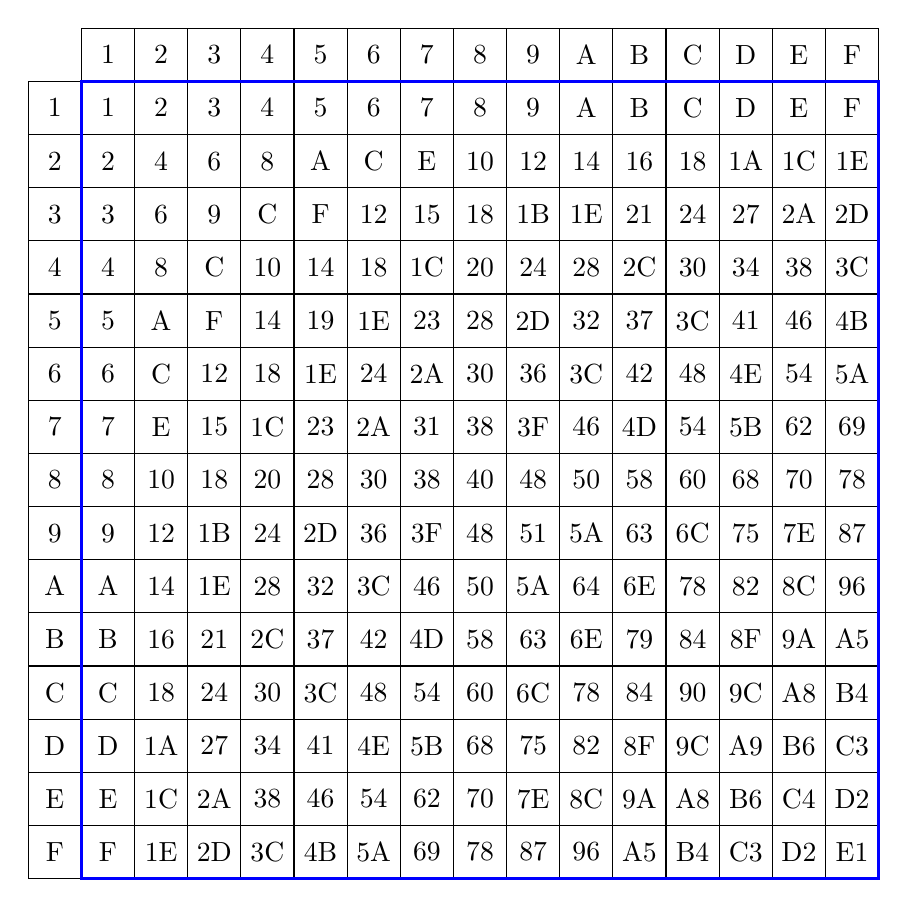
\begin{tikzpicture}[scale=0.675]
		% grid definition
		\draw (-1,0) grid (15,15);
		\draw (0,10) grid (15,16);
		\draw[line width=1pt, color=blue] (0,0) rectangle (15,15);
		
		% fill numbers
		\foreach \x in {1,2,3,...,15}
		\foreach \y in {1,2,3,...,15}
		\draw[shift={(-.5,-.5)}] (\x ,\y) node {\pgfmathHex{\number\numexpr\x*(16-\y)}\pgfmathresult\relax};
		
		% fill first row
		\foreach \x in {1,2,3,...,15}
		\draw[shift={(-.5,-.5)}] (\x , 16) node {\pgfmathHex{\x}\pgfmathresult};
		
		% fill first column
		\foreach \y in {1,2,3,...,15}
		\draw[shift={(-.5,-.5)}] (0, 16-\y) node {\pgfmathHex{\y}\pgfmathresult};
	\end{tikzpicture}
	\caption{Tavola Prodotti esadecimale}
	\label{tab:TavolaPitagoricaesadecimale}
\end{table}
\begin{table}[H]
	\centering
	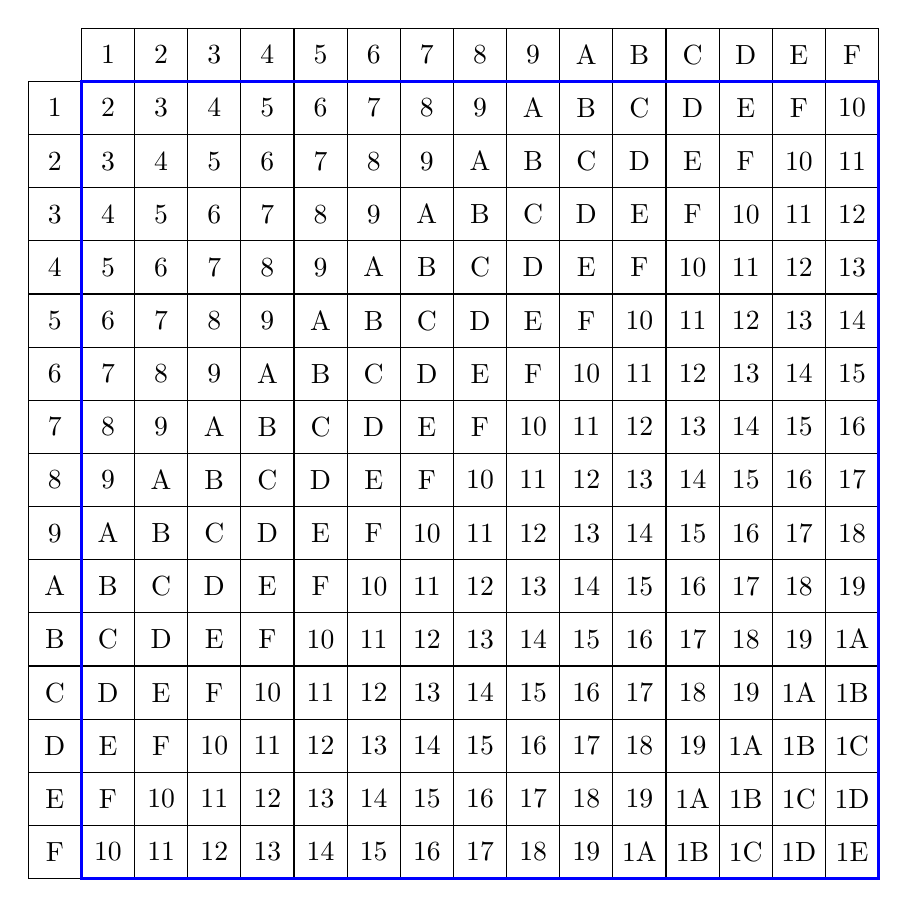
\begin{tikzpicture}[scale=0.675]
		% grid definition
		\draw (-1,0) grid (15,15);
		\draw (0,10) grid (15,16);
		\draw[line width=1pt, color=blue] (0,0) rectangle (15,15);
		
		% fill numbers
		\foreach \x in {1,2,3,...,15}
		\foreach \y in {1,2,3,...,15}
		\draw[shift={(-.5,-.5)}] (\x ,\y) node {\pgfmathHex{\number\numexpr\x+(16-\y)}\pgfmathresult\relax};
		
		% fill first row
		\foreach \x in {1,2,3,...,15}
		\draw[shift={(-.5,-.5)}] (\x , 16) node {\pgfmathHex{\x}\pgfmathresult};
		
		% fill first column
		\foreach \y in {1,2,3,...,15}
		\draw[shift={(-.5,-.5)}] (0, 16-\y) node {\pgfmathHex{\y}\pgfmathresult};
	\end{tikzpicture}
	\caption{Tavola somma esadecimale}
	\label{tab:Tavolaaddizioniesadecimale}
\end{table}
\subsection{Base otto}
\subsubsection{Conversioni}



\begin{table}[H]
	\centering
	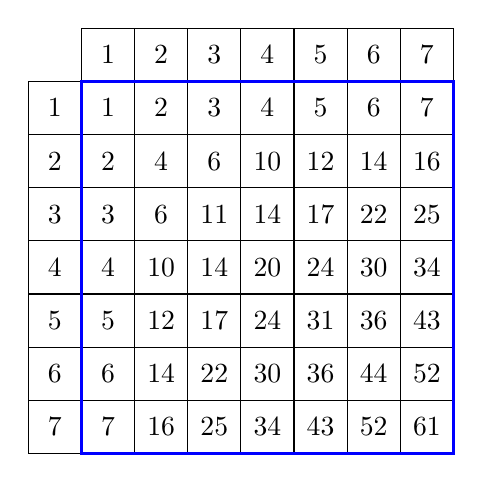
\begin{tikzpicture}[scale=0.675]
		% grid definition
		\draw (-1,0) grid (7,7);
		\draw (0,7) grid (7,8);
		\draw[line width=1pt, color=blue] (0,0) rectangle (7,7);
		
		% fill numbers
		\foreach \x in {1,2,3,...,7}
		\foreach \y in {1,2,3,...,7}
		\draw[shift={(-.5,-.5)}] (\x ,\y) node { \pgfmathoct{\number\numexpr\x*(8-\y)}\pgfmathresult\relax};
		
		% fill first row
		\foreach \x in {1,2,3,...,7}
		\draw[shift={(-.5,-.5)}] (\x , 8) node {\pgfmathoct{\x}\pgfmathresult};
		
		% fill first column
		\foreach \y in {1,2,3,...,7}
		\draw[shift={(-.5,-.5)}] (0, 8-\y) node {\pgfmathoct{\y}\pgfmathresult};
	\end{tikzpicture}
	\caption{Tavola Pitagorica ottale}
	\label{tab:TavolaPitagoricaottale}
\end{table}
\begin{table}[H]
	\centering
	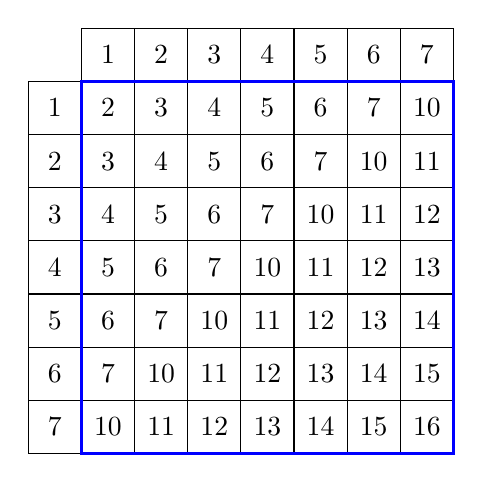
\begin{tikzpicture}[scale=0.675]
		% grid definition
		\draw (-1,0) grid (7,7);
		\draw (0,7) grid (7,8);
		\draw[line width=1pt, color=blue] (0,0) rectangle (7,7);
		
		% fill numbers
		\foreach \x in {1,2,3,...,7}
		\foreach \y in {1,2,3,...,7}
		\draw[shift={(-.5,-.5)}] (\x ,\y) node { \pgfmathoct{\number\numexpr\x+(8-\y)}\pgfmathresult\relax};
		
		% fill first row
		\foreach \x in {1,2,3,...,7}
		\draw[shift={(-.5,-.5)}] (\x , 8) node {\pgfmathoct{\x}\pgfmathresult};
		
		% fill first column
		\foreach \y in {1,2,3,...,7}
		\draw[shift={(-.5,-.5)}] (0, 8-\y) node {\pgfmathoct{\y}\pgfmathresult};
	\end{tikzpicture}
	\caption{Tavola Somma ottale}
	\label{tab:Tavolasommaottale}
\end{table}

	\chapter{Codifica Braille}
\label{Cha:CodificaBraille}
\begin{table}[H]
\begin{tabular}{cccc}
				\mytable{
					\braille{a} & a 1 \\
					\braille{b} & b 2 \\
					\braille{c} & c 3 \\
					\braille{d} & d 4 \\
					\braille{e} & e 5 \\
					\braille{f} & f 6 \\
					\braille{g} & g 7 \\
					\braille{h} & h 8 \\
					\braille{i} & i 9 \\
					\braille{j} & j 0 \\
					\braille{k} & k \\
					\braille{l} & l \\
					\braille{m} & m \\
					\braille{n} & n \\
					\braille{o} & o \\
				}&
				\mytable{
					\braille{p} & p \\
					\braille{q} & q \\
					\braille{r} & r \\
					\braille{s} & s \\
					\braille{t} & t \\
					\braille{u} & u \\
					\braille{v} & v \\
					\braille{w} & w \\
					\braille{x} & x \\
					\braille{y} & y \\
					\braille{z} & z \\
				}  &
				\mytable{
					\braille{{Capital}} & \{Maiuscolo\}\\
					\braille{{Upper}} & \{In alto\} \\
					%\braille{{Italic}} & \{Italic\} \\
				}
				&
				\mytable{
					\braille{{Number}} & \{Numero\} \\	
					\braille{{Letter}} & \{Lettera\} \\
				}   \\ 
				

			\end{tabular}
\caption[Codifica Braille]{ Codifica Braille (\copyright 1998-2010 William Park Licenza LPPL)}\label{tsd:}
\label{tab:CodificaBraille}
\end{table}
					
					
Ciao Mondo
					\braille{Ciao Mondo}
					
					1980
					\braille{{Number}1980}
	\input{extra/Cascii}
	\chapter{Algebra di Boole}
\label{cha:AlgebradiBoole}
%\FloatBarrier
\section{Variabili e funzioni booleane}
\label{sec:VariabiliBooleane}
Una variabile booleana\index{Variabile!booleana} è una variabile che può assumere solo due valori, che possono essere indicati o  con\nobs$0$\nobs e\nobs$1$ o con $basso$\nobs e\nobs$alto$, con $vero$\nobs o \nobs$falso$. Nella realtà, a questi valori sono  associati valori arbitrari es: $+5\si{\volt}$ $-5\si{\volt}$, $+12\si{\volt}$ $-12\si{\volt}$. 

 Un sistema si trova in un determinato stato a seconda del valore che assumono le variabili booleane associate.   Vi sono due variabili  particolari la variabile\nobs$0$ che assume solo il valore\nobs$0$ e la variabile \nobs$1$ che assume solo il valore\nobs$1$. 

Una funzione (operazione) booleana\index{Funzione!booleana} è una relazione  che ha in ingresso delle variabili indipendenti e in uscita una variabile dipendente.

A ogni sistema è associata una tabella detta tavola di verità\index{Tavola di verità}. Una tavola di verità rappresenta in forma tabellare, in base agli stati del sistema in entrata, lo stato del sistema in uscita. Si può facilmente provare %, utilizzando la tavola~\vref{tab:statisistema},  
che la tabella\vref{tab:totfunzzionilogiche} rappresenta tutte le funzioni logiche con due valori in entrata.

Due funzioni logiche sono equivalenti\index{Funzione!booleana!equivalente} se hanno la stessa tavola di verità. Esempio di questo sono la tabella\nobs\vref{tab:tabVeritaEOR} e la tabella\nobs\vref{tab:tabVeritaEOR2} che sono fra di loro equivalenti. 

Un metodo grafico per rappresentare una funzione logica  è il circuito che si ottiene combinando i simboli  elencati nella tabella\nobs\vref{tab:Portelogichetavver}. Un esempio di ciò sono  i due circuiti\nobs\vref{Tab:circuito2e3} che rappresentano entrambi la funzione $XOR$\index{Funzione!booleana!XOR}  ottenuta come combinazione di $AND$\index{Funzione!booleana!AND} e $OR$\index{Funzione!booleana!OR}

Principio di dualità: Se una funzione logica è vera, allora è vera la funzione che si ottiene scambiando $AND$ con  $OR$ e  $0$ con $1$ e viceversa.

\begin{table} %[H]
	%\centering
	\begin{tabular}{cccccccccccccccccc}
	\toprule
	A & B & $0$ & NOR & $\overline{A}$ &  &  & $\overline{B}$ & XOR & NAND & AND & XNOR &  & B & A &  & OR & $1$ \\ 
	\midrule
	1 & 1 & 0 & 0 & 0 & 0 & 0 & 0 & 0 & 0 & 1 & 1 & 1 & 1 & 1 & 1 & 1 & 1 \\ 
	1 & 0 & 0 & 0 & 0 & 0 & 1 & 1 & 1 & 1 & 0 & 0 & 0 & 0 & 1 & 1 & 1 & 1 \\ 
	0 & 1 & 0 & 0 & 1 & 1 & 0 & 0 & 1 & 1 & 0 & 0 & 1 & 1 & 0 & 0 & 1 & 1 \\ 
	0 & 0 & 0 & 1 & 1 & 0 & 0 & 1 & 0 & 1 & 0 & 1 & 1 & 0 & 0 & 1 & 0 & 1 \\ 
	\bottomrule
	\end{tabular}
	\caption{Funzioni logiche}
	\label{tab:totfunzzionilogiche}
\end{table}
\subsection{Esempi}
\label{sec:Esempiofunzlog}
Definire, utilizzando le funzioni logiche:

$tavolo=(legno,ferro,3gambe,4gambe,piano)$,

$auto=(3 porte,5 porte,ruote,motore)$, 

$penna=(sfera,stilografica,rossa,nera,verde,cancellabile,indelebile)$

Una cassaforte ha quattro lucchetti, x, y, v, w, che devono essere tutti aperti affinché la
cassaforte si apra.  Tre persone A, B, C,  hanno le  chiavi. A possiede le chiavi v e y; 
B ha le chiavi v e x e C tiene w e y. Le variabili A, B, C sono uguali a uno se la persona corrispondente è presente, altrimenti sono uguali a zero. Costruire la tavola
della verità della funzione $Y=f(A,B,C)$. La funzione  vale uno se e solo se la cassaforte può essere  aperta,
 esprimere f in forma algebrica. Per risolvere almeno la prima parte dell'esercizio costruiamo una tabella  che leghi le chiavi alle tre persone.
\begin{table}
	    \centering
		\begin{tabular}{c|cccc}
			& \textbf{x} & \textbf{y} &\textbf{v}& \textbf{w}\\
			\toprule 
			\textbf{A} &  & \textbullet &\textbullet & \\ 
			\textbf{B} & \textbullet &  & \textbullet& \\ 
			\textbf{C} &  & \textbullet & & \textbullet\\ 
			\bottomrule
		\end{tabular}
	\caption[]{Persone e chiavi}
	\label{tab:personeechiavi}
\end{table} 
Quindi: il sistema (la cassaforte aperta o chiusa), dipende da tre variabili $A$, $B$ e $C$ che assumono solo due valori $1$ se la chiave è presente o $0$ altrimenti. In uscita $Y$ può assumere due valori $1$ se la cassaforte è aperta o $0$ nell'altro caso. 

La tabella~\vref{tab:personeechiavi} permette di costruire la tavola di verità\nobs\vref{tab:tavolaveritacasaforte} della funzione. La tabella, dipendendo da tre variabili in ingresso, ha otto stati. Iniziamo a costruire la tavola di verità del sistema. Nella prima riga abbiamo che $A=0$, $B=0$ e $C=0$, poiché nessuna chiave è presente, la cassaforte rimane chiusa quindi $Y=0$. Nella seconda riga abbiamo che $A=0$, $B=0$ e $C=1$,  due chiavi sono presenti ma \nobs\vref{tab:personeechiavi} ci dice che queste non bastano e la cassaforte è chiusa e quindi $Y=0$. Il discorso è analogo  per le righe rimanenti. Nella riga quattro abbiamo che $A=0$, $B=1$ e $C=1$  sono presenti quattro chiavi e la cassaforte viene aperta per cui $Y=1$.  Stesso discorso la riga otto e anche in questo caso $Y=1$.
\begin{table}
		\centering
\begin{tabular}{c|c|c|c|c}
	& \textbf{A} & \textbf{B} & \textbf{C} & \textbf{Y} \\
	\toprule 
	1& 0 & 0 & 0 & 0 \\ 
	2& 0 & 0 & 1 &  0\\ 
	3& 0 & 1 & 0 &  0\\ 
	4& 0 & 1 & 1 &  1\\ 
	5& 1 & 0 & 0 &  0\\ 
	6& 1 & 0 & 1 &  0\\ 
	7& 1 & 1 & 0 &  0\\ 
	8& 1 & 1 & 1 &  1\\ 
	\bottomrule
\end{tabular} 
	\caption{Tavola di verità}
	\label{tab:tavolaveritacasaforte}
\end{table}
\section{Tavole di verità}
\label{sec:TavoleDiVeritA}
\begin{figure} %[H]
\centering
	\pagestyle{empty}
	% Set the overall layout of the tree
\tikzstyle{level 1}=[level distance=3.5cm, sibling distance=3.5cm]
\tikzstyle{level 2}=[level distance=3.5cm, sibling distance=2cm]
\tikzstyle{level 3}=[level distance=3cm, sibling distance=0.8cm] 
% Define styles for bags and leafs
%\tikzstyle{bag} = [text width=4em, text centered]
\tikzstyle{bag} =[shape=circle,draw,
text centered]
\begin{tikzpicture}[grow=right, sloped]
\matrix [row sep=1em] 
{
	\node[bag] {0}
	child{   
		node[bag] {0}
		child{
			node[bag] {0}
			child{
				node[bag]{0}
			}
			child{
				node[bag]{1}
			}
		}
		child {
			node[bag] {1}
			child{
				node[bag]{0}
			}
			child{
				node[bag]{1}
			}		
		}
	}
	child{
		node[bag]{1}
		child{
			node[bag] {0}
			child{
				node[bag]{0}
			}
			child{
				node[bag]{1}
			}
		}
		child {
			node[bag] {1}
			child{
				node[bag]{0}
			}
			child{
				node[bag]{1}
			}
		}   
	};
	&\\
	\draw (0,0) --  (10.5,0);
	\draw (0.0,1pt) -- (0.0,-3pt)
	node[anchor=north] {1};
	\draw (3.5,1pt) -- (3.5,-3pt)
	node[anchor=north] {2};
	\draw (7,1pt) -- (7,-3pt)
	node[anchor=north] {3};
	\draw (10,1pt) -- (10,-3pt)
	node[anchor=north] {4};\\
	\node[bag] {0}
	child{   
		node[bag] {0}
		child{
			node[bag] {0}
			child{
				node[bag]{0}
			}
			child{
				node[bag]{1}
			}
		}
		child {
			node[bag] {1}
			child{
				node[bag]{0}
			}
			child{
				node[bag]{1}
			}		
		}
	}
	child{
		node[bag]{1}
		child{
			node[bag] {0}
			child{
				node[bag]{0}
			}
			child{
				node[bag]{1}
			}
		}
		child {
			node[bag] {1}
			child{
				node[bag]{0}
			}
			child{
				node[bag]{1}
			}
		}   
	};\\
};
\end{tikzpicture}
	\caption{Stati del sistema}
	\label{tab:statisistema}
\end{figure}

Le funzioni logiche sono divise in gruppi. Il primo è formato dalle funzioni AND\index{Funzione!booleana!AND}, OR\index{Funzione!booleana!OR} e NOT\index{Funzione!booleana!NOT}. Segue il gruppo formato solo da NAND\index{Funzione!booleana!NAND}. Infine quello composto solo  da NOR\index{Funzione!booleana!NOR}. Ogni gruppo è tale perché in grado di generare le rimanenti funzioni. La figura~\vref{tab:Portelogichetavver} riporta le tavole di verità di queste funzioni. 

Combinando fra di loro le funzioni  otteniamo altre funzioni come viene per esempio, nella tabella~\vref{tab:ComposizionePorte}. 

La tabella~\vref{tab:statisistema} da in verticale di quante righe deve avere una tavola di verità.  Con una variabile due righe,  due variabili  otteniamo quattro righe etc. Mentre in orizzontale,in base al numero delle variabili, percorrendo i grafi da sinistra verso destra, avremo tutti i possibili stati di un sistema.
\subsection{Funzione AND}
\label{sub:funzioneAND}
La funzione AND\index{Funzione!booleana!AND} ha due valori in entrata ed  un valore in uscita che è vero solo quando sono veri entrambi i valori in entrata. Il simbolo che la rappresenta l'operazione è il prodotto.

Nella realtà casi in cui si usano funzioni AND sono molteplici. In genere si usa una funzione AND\index{Funzione!booleana!AND} quando  si eseguono due azioni in contemporaneamente come per esempio nel dispositivi di azionamento di una pressa in cui si premono contemporaneamente due pulsanti in modo da impegnare entrambe le mani, evitando così incidenti. 

Un esempio della funzione AND\index{Funzione!booleana!AND} è il seguente circuito\nobs\vref{tab:elettricoAND}. Abbiamo un circuito con due pulsanti in serie.  La lampada si accende solo premendo solo contemporaneamente i due interruttori.
\begin{table}[H]
	\centering
	\begin{circuitikz} \draw
		(0,0)--(0,2)
		(5,0)--(5,2)
		(0,0) to[lamp] (2,0)
		(2,0) to[battery] (5,0)
		(0,2) to[opening switch] (3,2)
		(3,2) to[opening switch] (5,2);
	\end{circuitikz}
	\caption{Circuito AND}
	\label{tab:elettricoAND}
\end{table}
	
La tabella\nobs\ref{tab:Portelogichetavver} mostra la tavola di verità\index{Tavola di verità!AND} della $AND$\index{Funzione!booleana!AND} e il simbolo grafico associato.
\subsection{Funzione OR}
\label{sub:funzioneOR}
La funzione OR\index{Funzione!booleana!OR} ha due valori in entrata e un valore in uscita. Questo valore è vero quando almeno uno dei valori in ingresso è vero. Il simbolo che la rappresenta è la somma. 

Un esempio dell'uso della funzione OR\index{Funzione!booleana!OR} è l'impianto di illuminazione di una stanza in cui due interruttori distinti permettono di accendere una lampadina.

Un circuito in parallelo, come il circuito\nobs\vref{tab:ZunzioneOR}, rappresenta la funzione OR\index{Funzione!booleana!OR}. Per accendere la lampadina basta premere almeno un interruttore.
\begin{table}
	\centering
	\begin{circuitikz} \draw
		(0,0)--(0,2)
		(5,0)--(5,2)
		(0,0) to[lamp] (2,0)
		(2,0) to[battery] (5,0)
		(0,2)--(1,2)
		(1,1)--(1,3)
		(4,1)--(4,3)
		(4,2)--(5,2)
		(1,3) to[opening switch] (4,3)
		(1,1) to[opening switch] (4,1);
	\end{circuitikz}
	\caption{Circuito OR}
	\label{tab:ZunzioneOR}
\end{table}
La tabella\nobs\ref{tab:Portelogichetavver} mostra la tavola di verità\index{Tavola di verità!OR} della OR\index{Funzione!booleana!OR} e il simbolo grafico associato.
\subsection{Funzione NOT}
\label{sub:funzionenot}
La funzione NOT ha un solo valore in entrata e un solo valore in uscita. Il valore in uscita è l'opposto a quello in ingresso. Il simbolo che rappresenta l'operazione è un trattino che si pone sopra la variabile.

Un esempio dell'uso della funzione NOT\index{Funzione!booleana!NOT} è per esempio l'interruttore della luce di cortesia di un'auto che si accende aprendo la portiera.

Un circuito come il circuito\nobs\vref{tab:CircuitoNOT} rappresenta la funzione NOT. La tabella\nobs\ref{tab:Portelogichetavver} mostra la tavola di verità\index{Tavola di verità!NOT} della NOT e il simbolo grafico associato.
\begin{table}
	\centering
	 \begin{circuitikz} \draw
		(0,0)--(0,2)
		(6,0)--(6,2)
		(0,1) to[lamp] (6,1)
		(0,2)--(3,2)
		(3,2) to[battery,v_<=$+-$] (6,2)
		(0,0) to[opening switch] (3,0)
		(3,0) to[battery,v_<=$+-$] (6,0);
	\end{circuitikz}
	\caption{Circuito NOT}
	\label{tab:CircuitoNOT}
\end{table}
	
\subsection{Funzione XOR}
\label{sub:funzioneXOR}
La funzione XOR\index{Funzione!booleana!XOR} ha due valori in entrata ed un valore in uscita che è vero quando solo uno dei valori in ingresso è vero.

Il circuito\nobs\vref{tab:circuitoXOR} rappresenta un OR esclusivo. Sono due gruppi di pulsanti in parallelo messe in serie. La seconda serie di pulsanti sono i negati dei precedenti. Quando vien premuto il primo pulsante $A$ il pulsante $\overline{A}$ del secondo circuito viene aperto e viceversa, analogamente per il pulsante $B$. In questo circuito la corrente passa e  lampadina si accende, solo se è premuto un solo pulsante ma non entrambi.

La tabella\nobs\ref{tab:Portelogichetavver} mostra la tavola di verità della XOR\index{Tavola di verità!XOR} e il simbolo grafico associato.
\begin{table} %[H]
		\centering
		\begin{circuitikz} \draw
			(0,0)--(0,2)
			(7,0)--(7,2)
			(0,0) to[lamp] (3,0)
			(3,0) to[battery] (7,0)
			(0,2)--(1,2)
			(1,1)--(1,3)
			(3,1)--(3,3)
			(3,2)--(4,2)
			(4,1)--(4,3)
			(6,1)--(6,3)
			(6,2)--(7,2)
			(1,3) to[opening switch=$A$] (3,3)
			(1,1) to[opening switch=$B$] (3,1)
			(4,1) to[closing switch=$\overline{B}$] (6,1)
			(4,3) to[closing switch=$\overline{A}$] (6,3);
		\end{circuitikz}
	\caption{Circuito XOR}
	\label{tab:circuitoXOR}
	\end{table}
\subsection{Funzione NAND}
\label{sub:funzioneNAND}
La funzione NAND\index{Funzione!booleana!NAND} ha due valori in entrata ed ha un valore in uscita che è falso solo quando sono veri entrambi i valori in entrata.

La tabella\nobs\ref{tab:Portelogichetavver} mostra la tavola di verità\index{Tavola di verità!NAND} della $NAND$\index{Funzione!booleana!NAND} e il simbolo grafico associato. La $NAND$ è la negazione di $AND$\index{Funzione!booleana!AND}.

\subsection{Funzione NOR}
\label{sub:funzioneNOR}
La funzione NOR\index{Funzione!booleana!NOR} ha due valori in entrata ed ha un valore in uscita che è vero solo quando sono falsi entrambi i valori in entrata.

La tabella\nobs\ref{tab:Portelogichetavver} mostra la tavola di verità\index{Tavola di verità!NOR} della NOR\index{Funzione!booleana!NOR} e il simbolo grafico associato. La NOR è la negazione di OR 
\subsection{Funzione XNOR}
\label{sub:funzioneXNOR}
La funzione XNOR\index{Funzione!booleana!XNOR} ha due valori in entrata ed ha un valore in uscita che è vero solo quando sono falsi entrambi i valori in entrata o quando sono entrambi veri. 

La tabella\nobs\ref{tab:Portelogichetavver} mostra la tavola di verità\index{Tavola di verità!XNOR} della XNOR e il simbolo grafico associato. La XNOR è la negazione di XOR 

Il circuito\nobs\vref{tab:circuitoXNOR} è formato da due blocchi di pulsanti in serie messi in parallelo. Quando vien premuto il primo pulsante $A$ il pulsante $\overline{A}$ del secondo circuito viene aperto e viceversa, analogamente per il pulsante $B$. La lampadina si accende o quando entrambi i pulsanti $A$ e $B$ sono premuti o entrambi i  pulsanti $A$ e $B$ sono tenuti alzati.
\begin{table}[H]
	\centering
	\begin{circuitikz} \draw
		(0,0)--(0,2)
		(7,0)--(7,2)
		(0,0) to[lamp] (3,0)
		(3,0) to[battery] (7,0)
		(0,2)--(1,2)
		(1,1)--(1,3)
		(6,1)--(6,3)
		(6,2)--(7,2)
		(1,3) to[opening switch=$A$] (4,3)
		(4,3) to[opening switch=$B$] (6,3)
		(1,1) to[closing switch=$\overline{A}$] (4,1)
		(4,1) to[closing switch=$\overline{B}$] (6,1);
	\end{circuitikz}
	\caption{Circuito XNOR}
	\label{tab:circuitoXNOR}
\end{table}
Come si è detto a una funzione logica è possibile associare una tavola di verità\index{Tavola di verità!Costruire}. Un esempio di costruzione  è la tabella~\vref{tab:tabVeritaEOR}. Il metodo usato è molto semplice,  prevede di suddividere la funzione nelle sue componenti e risolverle partendo da sinistra verso destra. Questo deve essere fatto rispettando le convenzioni di precedenza, cioè le negazioni (funzione NOT), poi i prodotti (Funzione AND\index{Funzione!booleana!AND}), e infine le somme (Funzione OR\index{Funzione!booleana!OR}).Possiamo cambiare le  precedenze mettendo fra  delle parentesi le operazioni che devono essere eseguite prima.
In conclusione, abbiamo parlato di tavola di verità\index{Tavola di verità}, circuito, funzione logica, che sono concetti fra loro equivalenti\vref{tab:FunzioneTavolaCircuito} e fra loro connessi.
\begin{table} 
	\centering
	\begin{tikzpicture}[very thick,node distance=5cm,text centered,minimum size=3cm]
		\node [circle, draw] (a) {Funzione logica};
		\node [circle, draw] (b) [above right=of a] {Tavola di verità};
		\node [circle, draw] (c) [above left=of a]{Circuito};
		\draw [<->] (a) to (b);
		\draw [<->] (b) to (c);
		\draw [<->] (c) to (a);
	\end{tikzpicture}
	\caption{Funzione, Tavola e Circuito}
	\label{tab:FunzioneTavolaCircuito}
\end{table}
\begin{table}
	\centering
	\begin{tabular}{@{}cc@{\hspace{2cm}}cc@{}}
	\begin{truthtable}{AND}
	\toprule
	$A$&$B$&$AB$\\
	\midrule           
	0&0&0\\
	1&0&0\\
	0&1&0\\
	1&1&1\\
	\bottomrule
	\end{truthtable}
	& \cport{and} &
	\begin{truthtable}{NAND}
	\toprule
	$A$&$B$&$A\mathbin{\overline{\wedge}}B$\\
	\midrule
	0&0&1\\
	1&0&1\\
	0&1&1\\
	1&1&0\\
	\bottomrule
	\end{truthtable}
	& \cport{nand} \\
	\addlinespace[3ex]
	\begin{truthtable}{OR}
	\toprule
	$A$&$B$&$A+B$\\
	\midrule         
	0&0&0\\
	1&0&1\\
	0&1&1\\
	1&1&1\\
	\bottomrule
	\end{truthtable}
	& \cport{or} &
	\begin{truthtable}{NOR}
	\toprule
	$A$&$B$&$A\mathbin{\overline{\vee}}B$\\
	\midrule
	0&0&1\\
	1&0&0\\
	0&1&0\\
	1&1&0\\
	\bottomrule
	\end{truthtable}
	& \cport{nor} \\
	\addlinespace[3ex]
	\begin{truthtable}{XOR}
	\toprule
	$A$&$B$&$A\XOR B$\\
	\midrule         
	0&0&0\\
	1&0&1\\
	0&1&1\\
	1&1&0\\
	\bottomrule
	\end{truthtable}
	& \cport{xor} &
	\begin{truthtable}{XNOR}
	\toprule
	$A$&$B$&$A\mathbin{\overline{\XOR}}B$\\
	\midrule
	0&0&1\\
	1&0&0\\
	0&1&0\\
	1&1&1\\
	\bottomrule
	\end{truthtable}
	& \cport{xnor} \\
	\addlinespace[3ex]
	\multicolumn{4}{c}{%
		\begin{tabular}{@{}cc@{}}
		\begin{truthtable}[2]{NOT}
		\toprule
		$A$&$\overline{A}$\\
		\midrule         
		0&1\\
		1&0\\
		\bottomrule
		\end{truthtable}
		& \cport{not}
		\end{tabular}}
	\end{tabular}
	\caption{Porte logiche}
	\label{tab:Portelogichetavver}
\end{table} 
\begin{table} %[H]
	\centering
	\begin{tabular}{ccc}
	\toprule
	\begin{circuitikz} \draw
	(0,0) node[and port] (myand) {}
	(1,0) node[not port] (mynot) {}
	(myand.out) -- (mynot.in)
	;\end{circuitikz}&&\begin{circuitikz} \draw
	(0,0) node[nor port]  {}
	;\end{circuitikz} \\
	AND +  NOT &=&NAND \\
	\midrule
	\begin{circuitikz} \draw
	(0,0) node[or port] (myor) {}
	(1,0) node[not port] (mynot) {}
	(myor.out) -- (mynot.in)
	;\end{circuitikz}&& \begin{circuitikz} \draw
	(0,0) node[nor port]  {}
	;\end{circuitikz} \\
	OR +  NOT &=&NOR  \\ 
	\midrule
	\begin{circuitikz} \draw
	(0,0) node[xor port] (myxor) {}
	(1,0) node[not port] (mynot) {}
	(myxor.out) -- (mynot.in)
	;\end{circuitikz}&& \begin{circuitikz} \draw
	(0,0) node[xnor port]  {}
	;\end{circuitikz} \\
	XOR +  NOT &=&XNOR  \\ 
	\bottomrule
	\end{tabular} 
	\caption{Composizione porte}%
	\label{tab:ComposizionePorte}%
\end{table}
\section{Proprietà dell'algebra algebra booleana}
\label{sec:Algebrabooleana}
La tabella\nobs\vref{Tab:AlgebrAbOOLEAN} elenca le principali proprietà delle funzioni AND\index{Funzione!booleana!AND} e OR\index{Funzione!booleana!OR} e mostra come le proprietà delle funzioni siano legate tramite il principio di dualità. Infatti, osservando la tabella si vede come le proprietà elencate a sinistra trovino il loro corrispondente duale a destra e viceversa. La tabella\nobs\vref{Tab:funzlogSemp} mostra come ottenere i risultati. Non vengono dimostrate tutte le relazioni inquarto le altre si ottengono per dualità.

%\altapriorita{Specificare meglio}
Una funzione logica non è unica ma può essere scritta in modi fra di loro equivalenti. La tabella\nobs\vref{Tab:funzlogSemp} mostra come con pochi passaggi si può passare da una funzione logica a una equivalente.
\begin{table}%[H]
\centering
\begin{tabular}{lcl}
\toprule
&PROPRIET\'A&\\
&$\overline{\overline{A}}=A$&\\
$A+0=A$&Elemento neutro&$A\cdot1=A$\\
$A+1=1$&Assorbimento&$A\cdot0=0$\\
$A+A=A$&Idempotenza&$A\cdot A=A$\\
$A+\overline{A}=1$&&$A\cdot\overline{A}=0$\\
$A+B=B+A$&Commutativa&$A\cdot B=B\cdot A$\\
$(A\cdot B)\cdot C=A\cdot(B\cdot C)=A\cdot B\cdot C$&Associativa&$(A+B)+C=A+(B+C)=A+B+C$\\
\midrule
&TEOREMI&\\
\midrule
$A+A\cdot B=A$&&$A\cdot(A+B)=A$\\
$A+\overline{A}\cdot B=A+B$&&$A\cdot (\overline{A}+B)=AB$\\
$(A+B)\cdot(A+C)=A+B\cdot C$&&$A\cdot B+A\cdot C=A\cdot(B+C)$\\
$(A+B)\cdot(\overline{A}+C)=\overline{A}\cdot B+A\cdot C$&&$A\cdot B+\overline{A}\cdot C=(\overline{A}+B)\cdot(A+B)$\\
\midrule
&TEOREMI DI DE MORGAN&\\
\midrule
$\overline{A+B}=\overline{A}\cdot\overline{B}$&&$\overline{A\cdot B}=\overline{A}+\overline{B}$\\
\bottomrule
\end{tabular}
\caption{Teoremi e proprietà algebra di Boole}%
\label{Tab:AlgebrAbOOLEAN}%
\end{table}
\begin{table}
\centering
\begin{tabular}{lcl}
\toprule
%\midrule
PROPRIET\'A&&DIMOSTRAZIONE\\
\midrule
$A+A\cdot B=A$&&$A+A\cdot B=$\\
&&$=A\cdot(1+B)=$\\
&&$=A\cdot1=A$\\ 
\midrule
$A+\overline{A}\cdot B=A+B$&&$A+A\cdot B+\overline{A}\cdot B=$\\
&&$=A+(A+\overline{A})\cdot B=$\\
&&$=A+1\cdot B=$\\
&&$=A+B$\\
\midrule
$(A+B)\cdot(A+C)=A+B\cdot C$&&$(A+B)\cdot(A+C)=$\\
&&$A\cdot A+A\cdot C+A\cdot B+B\cdot C=$\\
&&$=A+A\cdot C+A\cdot B+B\cdot C=$\\
&&$=A\cdot(1+C) +A\cdot B+B\cdot C=$\\
&&$=A\cdot 1 +A\cdot B+B\cdot C=$\\
&&$=A\cdot(1+B)+B\cdot C=$\\
&&$A+B\cdot C$\\
\midrule
$(A+B)\cdot(\overline{A}+C)=\overline{A}\cdot B+A\cdot C$&&$(A+B)\cdot(\overline{A}+C)$\\
&&$\overline{A}\cdot A+ A\cdot C +\overline{A}\cdot B+B\cdot A\cdot C$\\
&&$A\cdot B+\overline{A}\cdot B+B\cdot C$\\
&&$(A+B)\cdot C+\overline{A}\cdot B$\\
&&$(A+\overline{A}\cdot B)\cdot C+\overline{A}\cdot B$\\
&&$A\cdot C+\overline{A}\cdot B\cdot C+\overline{A}\cdot B$\\
&&$A\cdot C+\overline{A}\cdot B(C+1)$\\
&&$A\cdot C+\overline{A}\cdot B$\\
\bottomrule
\end{tabular}
\caption{Semplificazioni}
\label{Tab:funzlogSemp}
\end{table}
\section{Trovare la tavola di verità di una funzione}
\label{sec:Trovaretavolaveritàfunzione}
Per trovare data una funzione, la tavola di verità\index{Tavola di verità}, basta sostituire alle variabili booleane  i valori in ingresso e vedere cosa ha la funzione in uscita. 

Consideriamo la funzione $Y=A\cdot\overline{B}+\overline{A}\cdot B$  possiamo costruire la tabella\nobs\vref{tab:tabVeritaEOR} che fornisce tutti i calcoli necessari. Si procede sostituendo alle variabili tutti i valori possibili e ottenendo dopo i calcoli i risultati della colonna sette 

Analogo ragionamento è per $Y=(A+B)\cdot(\overline{A}+\overline{B})$ e ottenere la tabella\nobs\vref{tab:tabVeritaEOR2}.

Per $Y=\overline{A}\cdot\overline{B}\cdot C+\overline{A}\cdot B\cdot\overline{C}+\overline{A}\cdot B\cdot C+A\cdot B\cdot C$ otteniamo la tavola di verità\nobs\vref{Tab:esempio2bool}\index{Tavola di verità}

La tavola di verità per $Y=\overline{A}\cdot (A+B)+\overline{C}+B\cdot C$ e per $Y=B+\overline{C}$ è\nobs\vref{Tab:Tabveres1}
\begin{table}
	\centering
	\begin{tabular}{ccccccccccc}
		\toprule
		\multicolumn{10}{c}{$A\cdot\overline{B}+\overline{A}\cdot B$} \\ 
		&  &  & 1 & 3 & 2 & 7 & 4 & 6 & 5 \\ 
		A & B &  & $A$&$\cdot$  &$\overline{B}$&$+$& $\overline{A}$ &$\cdot$ &$B$  \\ 
		\cmidrule{1-2}\cmidrule{4-10}
		1 & 1 &  & 1 & 0 & 0 & 0 & 0 & 0 & 1 \\ 
		1 & 0 &  & 1 & 1 & 1 & 1 & 0 & 0 & 0 \\ 
		0 & 1 &  & 0 & 0 & 0 & 1 & 1 & 1 & 1 \\ 
		0 & 0 &  & 0 & 0 & 1 & 0 & 1 & 0 & 0 \\ 
		\bottomrule
	\end{tabular}
	\caption[]{Tavola di verità di $A\cdot\overline{B}+\overline{A}\cdot B$}
	\label{tab:tabVeritaEOR}
\end{table}
\begin{table}
	\centering
	\begin{tabular}{ccccccccccc}
		\toprule
		\multicolumn{10}{c}{$(A+B)\cdot(\overline{A}+\overline{B})$} \\ 
		&  &  & 1 & 3 & 2 & 7 & 4 & 6 & 5 \\ 
		A & B &  & $(A$&$+$  &$B)$ &$\cdot$ &$(\overline{A}$&$+$&$\overline{B})$  \\ 
		\cmidrule{1-2}\cmidrule{4-10}
		1 & 1 &  & 1 & 1 & 1 & 0 & 0 & 0 & 0 \\ 
		1 & 0 &  & 1 & 1 & 0 & 1 & 0 & 1 & 1 \\ 
		0 & 1 &  & 0 & 1 & 1 & 1 & 1 & 1 & 0 \\ 
		0 & 0 &  & 0 & 0 & 0 & 0 & 1 & 1 & 1 \\ 
		\bottomrule
	\end{tabular}
	\caption[]{Tavola di verità di $(A+B)\cdot(\overline{A}+\overline{B})$}
	\label{tab:tabVeritaEOR2}
\end{table}
\section{Trovare la funzione data la tavola di verità}
\label{sec:Trovarefunzionedatatavolaverità}
Per trovare la funzione, nota la tavola di verità\index{Tavola di verità!trovare!funzione}, possiamo utilizzare due metodi\footnote{I due metodi sono duali come si nota leggendo di seguito} 
\subsection{Somma di prodotti canonici} 
Per trovare data la tavola di verità la funzione si usa il metodo della somma di prodotti canonici\index{Somma prodotti canonici!\see{Mintermini}}. Ogni funzione logica si può scrivere come somma di prodotti detti mintermini\index{Mintermini}. Questi prodotti sono costituiti da prodotti di tutte le variabili in forma diretta o negata. Ogni mintermine assume il valore logico 1.

Nell'esempio uno si inizia dalla tavola\nobs\vref{Tab:esempio2bool},  si individuano le righe che hanno come risultato uno e si costruisce la somma dei mintermini. Nella riga due della tavola di verità si ha come risultato uno. Dato che le variabili $A$ $B$ assumono valore zero nel prodotto si inserisce il loro complemento e otteniamo $\overline{A}\cdot \overline{B}\cdot C$.

Si continua con lo stesso criterio ed otteniamo\[Y=2+3+4+8=\overline{A}\cdot\overline{B}\cdot C+\overline{A}\cdot B\cdot\overline{C}+\overline{A}\cdot B\cdot C+A\cdot B\cdot C\] cioè la funzione associata.
\begin{table}
	\centering
	\begin{tabular}{lccc|c}
		&A&B&C&Y\\
		\toprule
		1&0&0&0&0\\
		2&0&0&1&\textbf{1}\\
		3&0&1&0&\textbf{1}\\
		4&0&1&1&\textbf{1}\\
		5&1&0&0&0\\
		6&1&0&1&0\\
		7&1&1&0&0\\
		8&1&1&1&\textbf{1}\\
	\end{tabular}
	\caption[]{Tabella verità di $Y=\overline{A}\cdot\overline{B}\cdot C+\overline{A}\cdot B\cdot\overline{C}+\overline{A}\cdot B\cdot C+A\cdot B\cdot C$}
	\label{Tab:esempio2bool}
\end{table}
%\begin{table}
%	\begin{equation}
%	Y=2+3+4+8=\overline{A}\overline{B}C+\overline{A}B\overline{C}+\overline{A}BC+ABC
%	\end{equation}
%	\caption[]{Funzione booleana esempio 1}
%	\label{tab:esempio2funbool}
%\end{table}
\subsection{Prodotto di somme canoniche}
Per trovare, data la tavola di verità\index{Tavola di verità!trovare!funzione}, la funzione si usa il metodo della prodotti di somme  canoniche\index{Prodotti somme canoniche|see{Maxtermini} }. Ogni funzione logica si può scrivere come prodotto di somme detti maxtermini\index{Maxtermini}. Questi prodotti sono costituiti da somme di tutte le variabili in forma diretta o negata. Ogni maxtermine assume il valore logico 0.
Nell'esempio 1 si inizia dalla tavola\nobs\vref{Tab:esempio2bool}  si individuano le righe che hanno come risultato zero e si costruisce il prodotto dei maxtermini. Nella riga uno della tavola di verità si ha come risultato zero. Dato che le variabili $A$ $B$ $C$ assumono valore zero il max termine sarà $(A+B+C)$ 

Si continua con lo stesso criterio ed otteniamo\[Y=1+5+6+7=(A+B+C)(\overline{A}+B+C)(\overline{A}+B+ \overline{C})(\overline{A}+\overline{B}+C) \]
\section{Trovare il circuito corrispondente}
\label{Trovarecircuito}
\'E relativamente facile disegnare uno schema grafico che rappresenti un circuito. Partendo da \[Y=\overline{A}\cdot\overline{B}\cdot C+\overline{A}\cdot B\cdot\overline{C}+\overline{A}\cdot B\cdot C+A\cdot B\cdot C\] otteniamo\nobs\vref{tab:circuito1}. Il disegno è ottenuto ricordando le precedenza nelle operazioni per cui prima la negazione poi il prodotto e infine la somma.

I circuiti corrispondenti a \[(A+B)\cdot(\overline{A}+\overline{B})=A\cdot\overline{B}+\overline{A}\cdot B\] sono\nobs\vref{Tab:circuito2e3}
 In questo caso gli OR\index{Funzione!booleana!OR} hanno la precedenza perché contenuti in parentesi.
	
I circuiti corrispondenti a \[A\cdot B+\overline{A}\cdot\overline{B}=(\overline{A}+ B)\cdot(A+\overline{B})\] sono i circuiti disegnati in\nobs\vref{tab:circuito4e5}

Il circuito corrispondente a \[Y=\overline{A}\cdot (A+B)+\overline{C}+B\cdot C\] è il circuito disegnato in\nobs\vref{tab:circuito6}

Il circuito corrispondente a \[Y=\overline{A}\cdot C+\overline{A}\cdot B+B\cdot C\] è il circuito disegnato in\nobs\vref{tab:circuito7}
\begin{table}
\tikzstyle{branch}=[fill,shape=circle,minimum size=3pt,inner sep=0pt]
\centering
\begin{tikzpicture}
\node (A) at (0,0) {A};
\node (B) at (1,0) {B};
\node (C) at (2,0) {C};
\node[not gate US, draw] at ($(A)+(3,-2)$) (Not1) {};
\node[not gate US, draw] at ($(B)+(2,-1)$) (Not2) {};
\node[not gate US, draw] at ($(B)+(2,-2.5)$) (Not3) {};
\node[not gate US, draw] at ($(B)+(2,-3.4)$) (Not4) {};
\node[not gate US, draw] at ($(B)+(2,-3.9)$) (Not5) {};
\node[and gate US, draw, logic gate inputs=nnn, anchor=input 2] at ($(Not1.output-|Not2.output)+(1,.5)$) (and1){}; 
\node[and gate US, draw, logic gate inputs=nnn, anchor=input 3] at ($(Not3.output-|Not4.output)+(1,-.65)$) (and2){}; 
\node[and gate US, draw, logic gate inputs=nnn, anchor=input 3] at ($(Not5.output)+(1,-.4)$) (and3){}; 
\node[and gate US, draw, logic gate inputs=nnn, anchor=input 3] at ($(and3)+(-.4,-1.1)$) (and4){}; 
\node[or gate US, draw, logic gate inputs=nnnn, anchor=input 2] at ($(and2)+(3,-.5)$) (or1){};  
\draw (B)|-node[branch] {}(Not1.input);
\draw (A)|-node[branch] {}(Not2.input);
\draw(C)|-node[branch] {}(and1);
\draw(Not1.output)--([xshift=0.3cm]Not1.output) |-(and1.input 3);
\draw(Not2.output)--([xshift=0.3cm]Not2.output) |-(and1.input 1);
\draw (C)|-node[branch] {}(Not3.input);
\draw (A)|-node[branch] {}(Not4.input);
\draw(Not3.output)--([xshift=0.3cm]Not3.output) |-(and2.input 1);
\draw(Not4.output)--([xshift=0.3cm]Not4.output) |-(and2.input 3);
\draw(B)|-node[branch] {}(and2);
%
\draw(A)|-node[branch] {}(Not5.input);
\draw(Not5.output)--([xshift=0.3cm]Not5.output) |-(and3.input 1);
\draw(B)|-node[branch] {} (and3.input 2);
\draw(C)|-node[branch] {} (and3.input 3);
%
\draw(A)|-node[branch] {}(and4.input 1);
\draw(B)|- node[branch] {}(and4.input 2);
\draw(C)|- node[branch] {}(and4.input 3);
\draw(and1.output)--  ([xshift=0.5cm]and1.output) |- (or1.input 1);
\draw(and2.output)--([xshift=0.3cm]and2.output) |- (or1.input 2);
\draw(and3.output)--([xshift=0.3cm]and3.output) |- (or1.input 3);
\draw(and4.output)--  ([xshift=0.5cm]and4.output) |- (or1.input 4);
\draw (or1.output) -- ([xshift=0.5cm]or1.output) node[above] {};
\end{tikzpicture}
	\caption[]{Circuito corrispondente a $Y=\overline{A}\cdot\overline{B}\cdot C+\overline{A}\cdot B\cdot\overline{C}+\overline{A}\cdot B\cdot C+A\cdot B\cdot C$}
	\label{tab:circuito1}
\end{table}
\begin{table}
	%\centering
	\begin{circuitikz} \draw
		(0,0)--(0,4)
		(1,0)--(1,4)
		(0,0) node[anchor=east] {A}
		(1,0) node[anchor=east] {B}
		(5,3.0) node[or port] (myor1) {}
		
		(0,3.3)to[short, *-] (myor1.in 1)
		(1,2.7)to[short, *-](myor1.in 2)
		(2,1.8) node[not port] (mynot1) {}
		(0,1.8)to[short, *-](mynot1.in)
		(2,0.3) node[not port] (mynot2) {}
		(1,0.3)to[short, *-](mynot2.in)
		(5,1.1) node[or port] (myor2) {}
		(mynot1.out)-|(myor2.in 1)
		(mynot2.out)-|(myor2.in 2)
		(7.0,2.0) node[and port] (myand1) {}
		(myor1.out)-|(myand1.in 1)
		(myor2.out)-|(myand1.in 2);
	\end{circuitikz}
	\begin{circuitikz} \draw
		(0,0)--(0,4)
		(1,0)--(1,4)
		(0,0) node[anchor=east] {A}
		(1,0) node[anchor=east] {B}
		(5,3.0) node[and port] (myand1) {}
		(2,3.3) node[not port] (mynot1) {}
		(5,1.1) node[and port] (myand2) {}
		(2,0.8) node[not port] (mynot2) {}
		(7.0,2.0) node[or port] (myor1) {}	
		(0,3.3)to[short, *-] (mynot1.in)
		(mynot1.out)--(myand1.in 1)
		(1,2.7)to[short, *-](myand1.in 2)
		(0,3.3)to[short, *-](mynot1.in)
		(1,0.8)to[short, *-](mynot2.in)
		(0,1.4)to[short, *-](myand2.in 1)
		(mynot2.out)--(myand2.in 2)
		(myand1.out)-|(myor1.in 1)
		(myand2.out)-|(myor1.in 2);
	\end{circuitikz}
	\caption[]{Circuiti corrispondenti a $(A+B)\cdot(\overline{A}+\overline{B})=A\cdot\overline{B}+\overline{A}\cdot B$}
	\label{Tab:circuito2e3}
\end{table}
\begin{table} %[H]
	\begin{circuitikz} \draw
		(0,0)--(0,4)
		(1,0)--(1,4)
		(0,0) node[anchor=east] {A}
		(1,0) node[anchor=east] {B}
		(5,3.0) node[and port] (myand1) {}
		
		(0,3.3)to[short, *-] (myand1.in 1)
		(1,2.7)to[short, *-](myand1.in 2)
		(2,1.8) node[not port] (mynot1) {}
		(0,1.8)to[short, *-](mynot1.in)
		(2,0.3) node[not port] (mynot2) {}
		(1,0.3)to[short, *-](mynot2.in)
		(5,1.1) node[and port] (myand2) {}
		(mynot1.out)-|(myand2.in 1)
		(mynot2.out)-|(myand2.in 2)
		(7.0,2.0) node[or port] (myor1) {}
		(myand1.out)-|(myor1.in 1)
		(myand2.out)-|(myor1.in 2);
	\end{circuitikz}
	\begin{circuitikz} \draw
		(0,0)--(0,4)
		(1,0)--(1,4)
		(0,0) node[anchor=east] {A}
		(1,0) node[anchor=east] {B}
		(5,3.0) node[or port] (myor1) {}
		(2,3.3) node[not port] (mynot1) {}
		(5,1.1) node[or port] (myor2) {}
		(2,0.8) node[not port] (mynot2) {}
		(7.0,2.0) node[and port] (myand1) {}
		(0,3.3)to[short, *-] (mynot1.in)
		(mynot1.out)--(myor1.in 1)
		(1,2.7)to[short, *-](myor1.in 2)
		(0,3.3)to[short, *-](mynot1.in)
		(1,0.8)to[short, *-](mynot2.in)
		(0,1.4)to[short, *-](myor2.in 1)
		(mynot2.out)--(myand2.in 2)
		(myor1.out)-|(myand1.in 1)
		(myor2.out)-|(myand1.in 2);
	\end{circuitikz}
	\caption[]{Circuiti corrispondenti a $A\cdot B+\overline{A}\cdot\overline{B}=(\overline{A}+ B)\cdot(A+\overline{B})$}
	\label{tab:circuito4e5}
\end{table}
\begin{table}
	\tikzstyle{branch}=[fill,shape=circle,minimum size=3pt,inner sep=0pt]
	\centering
	\begin{tikzpicture}
	\node (A) at (0,0) {A};
	\node (B) at (0.5,0) {B};
	\node (C) at (1,0) {C};
	\node[not gate US, draw] at ($(A)+(2.1,-0.5)$) (not1) {};
	\node [or gate US, draw, logic gate inputs=nn, anchor=input 2]  at ($(A)+ (2,-1.8)$) (or1){};
	\node [and gate US, draw, logic gate inputs=nn, anchor=input 2]  at ($(not1.output-|or1.output)+(1,-0.7)$) (and1){};
	\node [and gate US, draw, logic gate inputs=nn, anchor=input 2]  at ($(not1.output-|or1.output)+(1,-2)$) (and2){};
	\node [or gate US, draw, logic gate inputs=nnn, anchor=input 2]  at ($(and1.output-|and2.output)+(2,-0.9)$) (or2){};
	\node [not gate US, draw]  at ($(not1.output-|or1.output)+(1.25,-3)$) (not2){};
	\draw(A)|-node[branch] {}(not1);
	\draw(A)|-node[branch] {}(or1.input 1);
	\draw(B)|-node[branch] {}(or1.input 2);
	\draw(not1.output) -- ([xshift=0.3cm]not1.output) |- (and1.input 1);
	\draw(or1.output) -- ([xshift=0.15cm]or1.output) |- (and1.input 2);
	\draw(B)|-node[branch] {}(and2.input 1);
	\draw(C)|-node[branch] {}(and2.input 2);
	\draw(C)|-node[branch] {}(not2.input);
	\draw(and1.output)--([xshift=0.3cm]and1.output)|-(or2.input 1);
	\draw(and2.output)--([xshift=0.3cm]and2.output)|-(or2.input 2);
	\draw(not2.output)--([xshift=0.4cm]not2.output)|-(or2.input 3);
	\draw (or2.output) -- ([xshift=0.5cm]or2.output) node[above] {};
	\end{tikzpicture}
	\caption[]{Circuito corrispondente a $Y=\overline{A}\cdot (A+B)+\overline{C}+B\cdot C$}
	\label{tab:circuito6}
\end{table}
\begin{table}
	\tikzstyle{branch}=[fill,shape=circle,minimum size=3pt,inner sep=0pt]
	\centering
	\begin{tikzpicture}
	\node (A) at (0,0) {A};
	\node (B) at (0.5,0) {B};
	\node (C) at (1,0) {C};
	\node[not gate US, draw] at ($(A)+(1.8,-1)$) (not1) {};
	\node [not gate US, draw] at ($(A)+(1.8,-1.8)$)(not2) {}; 
	\node [and gate US, draw, logic gate inputs=nn, anchor=input 1]  at ($(not1)+(1,0)$) (and1){};
	\node [and gate US, draw, logic gate inputs=nn, anchor=input 1]  at ($(not2)+(1,0)$) (and2){};
	\node [and gate US, draw, logic gate inputs=nn, anchor=input 1]  at ($(not2)+(1,-.75)$) (and3){};
	\node [or gate US, draw, logic gate inputs=nnn, anchor=input 2]  at ($(and1.output)+(1,-.8)$) (or1){};
	
	\draw(A)|-node[branch] {}(not1);
	\draw(B)|-node[branch] {}(and1.input 2);
	\draw(not1.output)--([xshift=0.3cm]not1.output)|-(and1.input 1);
	
	\draw(A)|-node[branch] {}(not2);
	\draw(C)|-node[branch] {}(and2.input 2);
	\draw(not2.output)--([xshift=0.3cm]not2.output)|-(and2.input 1);
	
	\draw(B)|-node[branch] {}(and3.input 1);
	\draw(C)|-node[branch] {}(and3.input 2);
	\draw(and1.output)--([xshift=0.3cm]and1.output)|-(or1.input 1);
	\draw(and2.output)--([xshift=0.3cm]and2.output)|-(or1.input 2);
	\draw(and3.output)--([xshift=0.3cm]and3.output)|-(or1.input 3);
	\draw (or1.output) -- ([xshift=0.5cm]or1.output) node[above] {};
	\end{tikzpicture}
	\caption[]{Circuito corrispondente a  $Y=\overline{A}\cdot C+\overline{A}\cdot B+B\cdot C$}
	\label{tab:circuito7}
\end{table}
\begin{table} %[htbp]
	\centering
	\begin{tabular}{lcl}
	\toprule
	EXOR&&EXNOR\\
	\midrule
	$(A+B)\cdot(\overline{A}+\overline{B})$&&$A\cdot B+\overline{A}\cdot\overline{B}$\\
	$A\cdot\overline{A}+A\cdot\overline{B}+\overline{A}\cdot B+B\cdot\overline{B}$&&\\
	$0+A\cdot\overline{B}+\overline{A}\cdot B+0$&&\\
	$A\cdot\overline{B}+\overline{A}\cdot B$&&$(\overline{A}+ B)\cdot(A+\overline{B})$\\
	\bottomrule
	\end{tabular}
	\caption{Funzioni EOR e EXNOR}
	\label{teb:funzexorexnor}
\end{table}
\section{Semplificazioni}
\label{sec:SEMPLIFICAZIONILOGICHE}
Per semplificazione si intende di individuare funzioni logiche più semplici rispetto a funzioni più complesse in partenza. Ovviamente queste funzioni devono essere equivalenti a quelle di partenza. Un esempio di questo è la trasformazione che viene presentata di seguito %a\nobs\vref{tab:esempio2semplificazione}
%\begin{table}
	\begin{align*}
	Y&=\overline{A}\cdot \overline{B}\cdot C+\overline{A}\cdot B\cdot \overline{C}+\overline{A}\cdot B\cdot C+A\cdot B\cdot C\\
	&&\overline{A}\cdot \overline{B} \cdot C=\overline{A}\cdot  \overline{B}\cdot C+\overline{A}\cdot \overline{B}\cdot C\\
	&&\overline{A}\cdot B\cdot \overline{C}=\overline{A}\cdot B\cdot \overline{C}+\overline{A}\cdot B\cdot\overline{C}\\
	&=\overline{A}\cdot \overline{B}\cdot C+\overline{A}\cdot B\cdot \overline{C}+\overline{A}\cdot B\cdot \overline{C}+\overline{A}\cdot B\cdot C+A\cdot B\cdot C+\overline{A}\cdot B\cdot C\\
	&=\overline{A}\cdot C\cdot (\overline{B}+B)+\overline{A}\cdot B\cdot (\overline{C}+C)+B\cdot C\cdot (A+\overline{A})\\
	&=\overline{A}\cdot C+\overline{A}\cdot B+B\cdot C\\
	\end{align*}
	%\caption[]{Semplificazione esempio 1}
	%\label{tab:esempio2semplificazione}
%\end{table}
\bassapriorita{Aggiungere esempi tabelle di verita e mappe}
\bassapriorita{Aggiungere esempi pratici}
\subsection{Esempio 1}
\label{sec:Esempio1semplificazioni}
\begin{align*}
Y&=\overline{A}\cdot (A+B)+\overline{C}+B\cdot C\\
 &=\overline{A}\cdot A+\overline{A}\cdot B+\overline{C}+B\cdot C\\
&&\overline{C}+C\cdot B=\overline{C}+B\\
&&\intertext{infatti prima dimostriamo che:}
&&\overline{C}+\overline{C}\cdot B=\overline{C}\\
&&\overline{C}\cdot (1+B)=\overline{C}\\
&&\intertext{quindi}
&&\overline{C}+B\cdot C=\overline{C}+\overline{C}\cdot B+B\cdot C\\
&&=\overline{C}+B\\
&=\overline{A}\cdot A+\overline{A}\cdot B+\overline{C}+B\\
&=0+B\cdot (\overline{A}+1)+\overline{C}\\
&=B\cdot 1+\overline{C}\\
&=B+\overline{C}\\
\end{align*}
\begin{table} %[htbp]
\centering
\begin{tabular}{ccc|c}
A&B&C&Y\\
\midrule
0&0&1&0\\
0&0&0&1\\
0&1&1&1\\
0&1&0&1\\
1&0&1&0\\
1&0&0&1\\
1&1&1&1\\
1&1&0&1\\
\bottomrule
\end{tabular}
\caption[]{Tavola di verità di $Y=\overline{A}\cdot (A+B)+\overline{C}+B\cdot C$ e $Y=B+\overline{C}$}
\label{Tab:Tabveres1}
\end{table}
\begin{table}
\centering
\tikzstyle{branch}=[fill,shape=circle,minimum size=3pt,inner sep=0pt]
\begin{tikzpicture}
\node (B) at (0,0) {B};
\node (C) at (0.5,0) {C};

\node[not gate US, draw] at ($(B)+(2,-1)$) (not1) {};
\node[or gate US, draw, logic gate inputs=nnn, anchor=input 2] at ($(not1)+(1,-.14)$) (or1){};  

\draw (C)|-node[branch] {}(not1.input);
\draw (B)|-node[branch] {}(or1.input 3);
\draw(not1.output)|-(or1.input 1);
\draw (or1.output) -- ([xshift=0.5cm]or1.output) node[above] {};
\end{tikzpicture}
\caption[]{Circuito corrispondente a $Y=B+\overline{C}$}
\label{tab:circuito8}
\end{table}
\subsection{Esempio 2}
\label{secEsempio3logbool}
\begin{align*}
Y&=\overline{A+A\cdot \overline{B}+C\cdot D}\\
&=\overline{A\cdot (1+\overline{B})+C\cdot D}\\
&=\overline{A+C\cdot D}\\
&=\overline{A}\cdot\overline{C\cdot D}\\
&=\overline{A}\cdot (\overline{C}+\overline{D})\\
\end{align*}
 \begin{table}
 \centering
 \tikzstyle{branch}=[fill,shape=circle,minimum size=3pt,inner sep=0pt]
 \begin{tikzpicture}
 \node (A) at (0,0) {A};
 \node (B) at (0.5,0) {B};
 \node (C) at (1,0) {C};
 \node (D) at (1.5,0) {D};
 \node[not gate US, draw] at ($(B)+(2,-.5)$) (not1) {};
 
 \node[and gate US, draw, logic gate inputs=nnn, anchor=input 2] at ($(not1)+(1,-.15)$) (and1){};  
 \node[and gate US, draw, logic gate inputs=nnn, anchor=input 2] at ($(not1)+(1,-1)$) (and2){};  
 \node[or gate US, draw, logic gate inputs=nnn, anchor=input 2] at ($(and2.output|-and1.output)+(1,-.4)$) (or1){};  
 \node[not gate US, draw] at ($(or1)+(1,0)$) (not2) {};
 %\draw (B)|-node[branch] {}(Not1.input);
 \draw (A)|-node[branch] {}(not1.input);
 \draw (B)|-node[branch] {}(and1.input 3);
 \draw (C)|-node[branch] {}(and2.input 1);
 \draw (D)|-node[branch] {}(and2.input 3);
 \draw (A)|-node[branch] {}(or1.input 2);
 \draw(not1.output)|-(and1.input 1);
 \draw(and1.output)--([xshift=0.3cm]and1.output)|-(or1.input 1);
 \draw(and2.output)--([xshift=0.3cm]and2.output)|-(or1.input 3);
 \draw(or1.output)--(not2);
 \draw (not2.output) -- ([xshift=0.5cm]not2.output) node[above] {};
 \end{tikzpicture}
 	\caption[]{Circuito corrispondente a $Y=\overline{A+A\cdot \overline{B}+C\cdot D}$}
 	\label{tab:circuito9}
 \end{table}
 
 \begin{table}
 	\tikzstyle{branch}=[fill,shape=circle,minimum size=3pt,inner sep=0pt]
 	\centering
 	\begin{tikzpicture}
 	\node (A) at (0,0) {A};
 	\node (B) at (0.5,0) {B};
 	\node (C) at (1,0) {C};
 	\node (D) at (1.5,0) {D};
 	\node[not gate US, draw] at ($(B)+(2,-.5)$) (not1) {};
 	\node[not gate US, draw] at ($(not1)+(0,-.5)$) (not2) {};
 	\node[not gate US, draw] at ($(not1)+(0,-1)$) (not3) {};
 	\node[or gate US, draw, logic gate inputs=nnn, anchor=input 2] at ($(not1)+(1,-.25)$) (or1){};  
 	\node[and gate US, draw, logic gate inputs=nnn, anchor=input 2] at ($(or1)+(1,-.5)$) (and1){};  
 	\draw (C)|-node[branch] {}(not1.input);
 	\draw (D)|-node[branch] {}(not2.input);
 	\draw(not1.output)--([xshift=0.3cm]not1.output)|-(or1.input 1);
 	\draw(not2.output)--([xshift=0.3cm]not2.output)|-(or1.input 3);
 	\draw(or1.output)--([xshift=0.3cm]or1.output)|-(and1.input 1);
 	\draw (A)|-node[branch] {}(not3.input);
 	\draw(not3.output)--([xshift=0.3cm]not3.output)|-(and1.input 3);
 	\draw (and1.output) -- ([xshift=0.5cm]and1.output) node[above] {};
 	\end{tikzpicture}
 	\caption[]{Circuito corrispondente a $Y=\overline{A}\cdot (\overline{C}+\overline{D}$)}
 	\label{tab:circuito10}
 \end{table}
\section{Solo NOR}
\label{sec:Solonor}

\begin{table} %[H]
	\centering
	\begin{tabular}{llc}
		\toprule
		NOT& $\overline{A}=A\overline{\vee} A$&\tikzstyle{branch}=[fill,shape=circle,minimum size=3pt,inner sep=0pt]
		\begin{tikzpicture}
		\node (A) at (0,0) {A};
		\node[nor gate US, draw, logic gate inputs=nnn, anchor=input 2] at ($(A)+(1,0)$) (nor1){};  
		\draw(nor1.input 1)--([xshift=-0.3cm]nor1.input 1)|-(nor1.input 3);
		\draw(A)|-node[branch] {}([xshift=-0.3cm]nor1.input 2);
		\end{tikzpicture}\\
		OR&$A+B=\overline{A\overline{\vee} B}$&\tikzstyle{branch}=[fill,shape=circle,minimum size=3pt,inner sep=0pt]
		\begin{tikzpicture}
		\node (A) at (0,0) {A};
		\node(B) at (.5,0){B};
		\node[nor gate US, draw, logic gate inputs=nnn, anchor=input 2] at ($(A)+(1,0)$) (nor1){};  
		\node[nor gate US, draw, logic gate inputs=nnn, anchor=input 2] at ($(nor1)+(1.5,0)$) (nor2){};  
		\draw(nor2.input 1)--([xshift=-0.3cm]nor2.input 1)|-(nor2.input 3);
		\draw(A)|-node[branch] {}(nor1.input 1);
		\draw(B)|-node[branch] {}(nor1.input 3);
		\draw(nor1.output)--([xshift=-0.3cm]nor2.input 2);
		\end{tikzpicture}\\
		AND&$A\cdot B=\overline{\overline{A}\overline{\vee} \overline{B}}$&\tikzstyle{branch}=[fill,shape=circle,minimum size=3pt,inner sep=0pt]
		\begin{tikzpicture}
		\node (A) at (0,0) {A};
		\node[nor gate US, draw, logic gate inputs=nnn, anchor=input 2] at ($(A)+(1,0
		)$) (nor1){};  
		\draw(nor1.input 1)--([xshift=-0.3cm]nor1.input 1)|-(nor1.input 3);
		\draw(A)|-node[branch] {}([xshift=-0.3cm]nor1.input 2);
		\node (B) at (0,-1) {B};
		\node[nor gate US, draw, logic gate inputs=nnn, anchor=input 2] at ($(B)+(1,0)$) (nor2){};  
		\draw(nor2.input 1)--([xshift=-0.3cm]nor2.input 1)|-(nor2.input 3);
		\draw(B)|-node[branch] {}([xshift=-0.3cm]nor2.input 2);
		\node[nor gate US, draw, logic gate inputs=nnn, anchor=input 2] at ($(nor1.output)+(1,-.5)$) (nor3){};
		\draw(nor1.output)--([xshift=0.5cm]nor1.output)|-(nor3.input 1); 
		\draw(nor2.output)--([xshift=0.5cm]nor2.output)|-(nor3.input 3);
		\end{tikzpicture} \\
		\bottomrule
	\end{tabular}
	\caption{Solo NOR}
	\label{Tab:solonor}
\end{table}
\section{Solo NAND}
\label{sec:SoloNAND}
\begin{table} %[H]
	\centering
	\begin{tabular}{llc}
		\toprule
		NOT& $\overline{A}=A\overline{\vee} A$&\tikzstyle{branch}=[fill,shape=circle,minimum size=3pt,inner sep=0pt]
		\begin{tikzpicture}
		\node (A) at (0,0) {A};
		\node[nand gate US, draw, logic gate inputs=nnn, anchor=input 2] at ($(A)+(1,0)$) (nand1){};  
		\draw(nand1.input 1)--([xshift=-0.3cm]nand1.input 1)|-(nand1.input 3);
		\draw(A)|-node[branch] {}([xshift=-0.3cm]nand1.input 2);
		\end{tikzpicture}\\
		OR&$A+B=\overline{A\overline{\vee} B}$&\tikzstyle{branch}=[fill,shape=circle,minimum size=3pt,inner sep=0pt]
		\begin{tikzpicture}
		\node (A) at (0,0) {A};
		\node(B) at (.5,0){B};
		\node[nand gate US, draw, logic gate inputs=nnn, anchor=input 2] at ($(A)+(1,0)$) (nand1){};  
		\node[nand gate US, draw, logic gate inputs=nnn, anchor=input 2] at ($(nand1)+(1.5,0)$) (nand2){};  
		\draw(nand2.input 1)--([xshift=-0.3cm]nand2.input 1)|-(nand2.input 3);
		\draw(A)|-node[branch] {}(nand1.input 1);
		\draw(B)|-node[branch] {}(nand1.input 3);
		\draw(nand1.output)--([xshift=-0.3cm]nand2.input 2);
		\end{tikzpicture}\\
		AND&$A\cdot B=\overline{\overline{A}\overline{\vee} \overline{B}}$&\tikzstyle{branch}=[fill,shape=circle,minimum size=3pt,inner sep=0pt]
		\begin{tikzpicture}
		\node (A) at (0,0) {A};
		\node[nand gate US, draw, logic gate inputs=nnn, anchor=input 2] at ($(A)+(1,0
		)$) (nand1){};  
		\draw(nand1.input 1)--([xshift=-0.3cm]nand1.input 1)|-(nand1.input 3);
		\draw(A)|-node[branch] {}([xshift=-0.3cm]nand1.input 2);
		\node (B) at (0,-1) {B};
		\node[nand gate US, draw, logic gate inputs=nnn, anchor=input 2] at ($(B)+(1,0)$) (nand2){};  
		\draw(nand2.input 1)--([xshift=-0.3cm]nand2.input 1)|-(nand2.input 3);
		\draw(B)|-node[branch] {}([xshift=-0.3cm]nand2.input 2);
		\node[nand gate US, draw, logic gate inputs=nnn, anchor=input 2] at ($(nand1.output)+(1,-.5)$) (nand3){};
		\draw(nand1.output)--([xshift=0.5cm]nand1.output)|-(nand3.input 1); 
		\draw(nand2.output)--([xshift=0.5cm]nand2.output)|-(nand3.input 3);
		\end{tikzpicture} \\
		\bottomrule
	\end{tabular}
	\caption{Solo NAND}
	\label{Tab:solonand1}
\end{table}



	%\newgeometry{bottom=1cm,top=1cm}
\chapter{Filtri Passivi primo ordine}
\label{cha:Filtripassiviprimoord}
\begin{table}[t]
\centering
     \begin{minipage}{0.4\textwidth}
      \centering
       \includegraphics{extra/filtri/filtro_PA_CR}
\centering
 \begin{align*}
A&=\dfrac{V_{u}}{V_{i}}
=\dfrac{R}{R+\dfrac{1}{J2\pi fC}}=\\
&=\dfrac{J2\pi fRC}{1+J2\pi cfRC}=
\dfrac{1}{1+\dfrac{1}{J2\pi fRC}}\\
f_{c}&=\dfrac{1}{2\pi RC}
        \end{align*}
       \end{minipage}\hfill
\begin{minipage}[t]{0.4\textwidth}
      \centering
\includegraphics{extra/filtri/filtro_PA_RL}
\centering
     \begin{align*}
A&=\dfrac{V_{u}}{V_{i}}&=\dfrac{J2\pi fL}{R+J2\pi cfL}=\\
\dfrac{J2\pi f\dfrac{L}{R}}{1+J2\pi f\dfrac{L}{R}}
&=\dfrac{1}{1+\dfrac{1}{J2\pi f\dfrac{L}{R}}}\\
f_{c}&=\dfrac{1}{2\pi \dfrac{L}{R}}
        \end{align*}
     \end{minipage}
 \begin{subfigure}[b]{.5\linewidth}
 	\centering\includegraphics[scale=0.6]{extra/filtri/filtropa}
 	\caption{Filtro PA Grafico}
 \end{subfigure}
%\subfloat[][Filtro PA Grafico]{
%\centering
%  \includegraphics[scale=0.6]{filtropa}}
\caption{Filtro passa alto}
\label{tab:filtropassaalto}
\end{table}
\begin{table} %[htbp]
\centering
\begin{minipage}{0.4\textwidth}
      \centering
     \includegraphics{extra/filtri/filtro_PB_LR}
\centering
 \begin{align*}
A&=\dfrac{V_{u}}{V_{i}}
=\dfrac{R}{R+J2\pi fL}\\
&=\dfrac{1}{1+J2\pi f\dfrac{L}{R}}\\
f_{c}&=\dfrac{1}{2\pi \dfrac{L}{R}}
        \end{align*} 
 \end{minipage}\hfill
  \begin{minipage}{0.4\textwidth}
      \centering
\includegraphics{extra/filtri/filtro_PB_RC}
  \centering
\begin{align*}
A&=\dfrac{V_{u}}{V_{i}}
=\dfrac{\dfrac{1}{J2\pi fc}}{R+\dfrac{1}{J2\pi fC}}=\\
&=\dfrac{1}{1+J2\pi fRC}\\
f_{c}&=\dfrac{1}{2\pi RC}
        \end{align*}
       %\caption{Passa Basso}
     \end{minipage}
  \begin{subfigure}[b]{.5\linewidth}
  	\centering\includegraphics[scale=0.6]{extra/filtri/filtropb}
  	\caption{Filtro PA Grafico}
  \end{subfigure}
%\subfloat[][Filtro PA Grafico]{
%\centering
%  \includegraphics[scale=0.6]{filtropb}}
\caption{Filtro passa basso}
\label{tab:filtropassabasso}
\end{table}



	\chapter{Funzioni Sinusoidali}
\label{sec:FunzioniSinusoidali}
\altapriorita{Inserire testo}
\begin{figure}
	\begin{subfigure}[b]{.5\linewidth}
		\centering\includestandalone[width=7.5cm]{extra/gonio/funzgonioTikz/asinomegat}
		\caption{Grafico di $y=A\sin\omega t$}\label{fig:asinomegat}
	\end{subfigure}%
	\qquad\qquad
	\begin{subfigure}[b]{.5\linewidth}
		\centering\includestandalone[width=7.5cm]{extra/gonio/funzgonioTikz/acosomegat}
		\caption{Grafico di $y=A\cos\omega t$}\label{fig:acosomegat}
	\end{subfigure}
	\caption{Funzioni sinusoidali}
	\label{fig:Funzionisinusoidali}
\end{figure}
\begin{figure}
	\begin{subfigure}[b]{.5\linewidth}
		\centering\includestandalone[width=7.5cm]{extra/gonio/funzgonioTikz/asinomegadiversit}
		\caption{Funzioni di frequenze diverse}\label{fig:frequenzediverse}
	\end{subfigure}%
		\qquad\qquad
	\begin{subfigure}[b]{.5\linewidth}
		\centering\includestandalone[width=7.0cm]{extra/gonio/funzgonioTikz/ampiezzediverse}
		\caption{Funzioni di ampiezze diverse}\label{fig:ampiezzediverse}
	\end{subfigure}
	\caption{Confronto fra funzioni di frequenza o ampiezza diverse}
	\label{fig:ampiezzediversefrequenzediverse}
\end{figure}
\begin{figure}
	\begin{subfigure}[b]{.5\linewidth}
		\centering\includestandalone[width=7.5cm]{extra/gonio/funzgonioTikz/AsinomegaTSfasamentoAnticipato}
		\caption{Funzioni in anticipo di fase}\label{fig:AsinomegaTSfasamentoAnticipato}
	\end{subfigure}%
		\qquad\qquad
	\begin{subfigure}[b]{.5\linewidth}
		\centering\includestandalone[width=7.5cm]{extra/gonio/funzgonioTikz/AsinomegaTSfasamentoRitardato}
		\caption{Funzioni in ritardo di fase}\label{fig:AsinomegaTSfasamentoRitardato}
	\end{subfigure}
	\caption{Funzioni che differiscono per la fase}%
	\label{fig:Funzionichedifferisconoperlafase}%
\end{figure}
\begin{figure}
	\begin{subfigure}[b]{0.5\linewidth}
		\centering\includestandalone[width=7.5cm]{extra/gonio/funzgonioTikz/AsinAnticipoDiFase}
		\caption{Quadratura di fase in anticipo}\label{fig:QuadraturaFaseAnticipo}
	\end{subfigure}%
		\qquad\qquad
	\begin{subfigure}[b]{0.5\linewidth}
		\centering\includestandalone[width=7.5cm]{extra/gonio/funzgonioTikz/AsinRitardoDiFase}
		\caption{Quadratura di fase in ritardo}\label{fig:QuadraturaFaseARitardo}
	\end{subfigure}
	\begin{subfigure}[b]{0.5\linewidth}
			\centering\includestandalone[width=7.5cm]{extra/gonio/funzgonioTikz/opposizionedifase}
			\caption{Opposizione di fase}\label{fig:Opposizionedifase}
	\end{subfigure}
	\caption{Funzioni in quadratura e opposizione}%
	\label{fig:Funzioniinquadratura}%
\end{figure}

% Tikz File 'mytikz.tex'
\documentclass{standalone}
\input{../Mod_base/grafica}

%\usetikzlibrary{...}
\begin{document}
	

		\begin{tikzpicture}[cap=round,>=latex,scale=5.3]
		% draw the coordinates
		\draw[->] (-1.5cm,0cm) -- (1.5cm,0cm) node[right,fill=white] {$x$};
		\draw[->] (0cm,-1.5cm) -- (0cm,1.5cm) node[above,fill=white] {$y$};
		
		% draw the unit circle
		\draw[thick] (0cm,0cm) circle(1cm);
		
		\foreach \x in {0,30,...,360} {
			% lines from center to point
			\draw[gray] (0cm,0cm) -- (\x:1cm);
			% dots at each point
			\filldraw[black] (\x:1cm) circle(0.4pt);
			% draw each angle in degrees
			\draw (\x:0.6cm) node[fill=white] {$\x^\circ$};
		}
		% draw each angle in radians
		\foreach \x/\xtext in {
			30/\dfrac{\pi}{6},
			45/\dfrac{\pi}{4},
			60/\dfrac{\pi}{3},
			90/\dfrac{\pi}{2},
			120/\dfrac{2\pi}{3},
			135/\dfrac{3\pi}{4},
			150/\dfrac{5\pi}{6},
			180/\pi,
			210/\dfrac{7\pi}{6},
			225/\dfrac{5\pi}{4},
			240/\dfrac{4\pi}{3},
			270/\dfrac{3\pi}{2},
			300/\dfrac{5\pi}{3},
			315/\dfrac{7\pi}{4},
			330/\dfrac{11\pi}{6},
			360/2\pi}
		\draw (\x:0.85cm) node[fill=white] {$\xtext$};
		
		\foreach \x/\xtext/\y in {
			% the coordinates for the first quadrant
			30/\dfrac{\sqrt{3}}{2}/\dfrac{1}{2},
			45/\dfrac{\sqrt{2}}{2}/\dfrac{\sqrt{2}}{2},
			60/\dfrac{1}{2}/\dfrac{\sqrt{3}}{2},
			% the coordinates for the second quadrant
			150/-\dfrac{\sqrt{3}}{2}/\dfrac{1}{2},
			135/-\dfrac{\sqrt{2}}{2}/\dfrac{\sqrt{2}}{2},
			120/-\dfrac{1}{2}/\dfrac{\sqrt{3}}{2},
			% the coordinates for the third quadrant
			210/-\dfrac{\sqrt{3}}{2}/-\dfrac{1}{2},
			225/-\dfrac{\sqrt{2}}{2}/-\dfrac{\sqrt{2}}{2},
			240/-\dfrac{1}{2}/-\dfrac{\sqrt{3}}{2},
			% the coordinates for the fourth quadrant
			330/\dfrac{\sqrt{3}}{2}/-\dfrac{1}{2},
			315/\dfrac{\sqrt{2}}{2}/-\dfrac{\sqrt{2}}{2},
			300/\dfrac{1}{2}/-\dfrac{\sqrt{3}}{2}}
		\draw (\x:1.25cm) node[fill=white] {$\left(\xtext,\y\right)$};
		
		% draw the horizontal and vertical coordinates
		% the placement is better this way
		\draw (-1.25cm,0cm) node[above=1pt] {$(-1,0)$}
		(1.25cm,0cm)  node[above=1pt] {$(1,0)$}
		(0cm,-1.25cm) node[fill=white] {$(0,-1)$}
		(0cm,1.25cm)  node[fill=white] {$(0,1)$};
		\end{tikzpicture}
\end{document}
\chapter{Tabelle Goniometriche}
\label{cha:TabelleGoniometriche}
\begin{table}[H]
%	\footnotesize
	\centering
	\renewcommand{\arraystretch}{3}
	\begin{tabular}{cccccc}
		\toprule
		Gradi & Radianti & Seno & Coseno & Tangente & Cotangente \\ [.25cm]
		\midrule
		$\ang{0}$ & 0 & 0 & 1 & 0 & n.e. \\ [.25cm] 
		%\hline%
		%$\ang{15}$ &$\dfrac{1}{12}\pi$ &$\dfrac{1}{4}\left(\sqrt{6}-\sqrt{2}\right)$&$\dfrac{1}{4}\left(\sqrt{6}+\sqrt{2}\right)$&$2-\sqrt{3}$& $2+\sqrt{3}$ \\ [.25cm]
		%\hline%
		%$\ang{18}$&$\dfrac{1}{10}\pi$& $\dfrac{1}{4}\left(\sqrt{5}-1\right)$ & $\dfrac{1}{4}\sqrt{10+2\sqrt{5}}$ & $\dfrac{1}{5}\sqrt{25-10\sqrt{5}}$ & $\sqrt{5+2\sqrt{5}}$ \\ [.25cm]
		%\hline%
		% $\ang{22;30;}$&$\dfrac{1}{8}\pi$&$\dfrac{1}{2}\sqrt{2-\sqrt{2}}$&$\dfrac{1}{2}\sqrt{2+\sqrt{2}}$&$\sqrt{2}-1$&$\sqrt{2}+1$ \\ [.25cm]
		\hline%
		$\ang{30}$&$\dfrac{1}{6}\pi$&$\dfrac{1}{2}$&$\dfrac{\sqrt{3}}{2}$&$\dfrac{\sqrt{3}}{3}$&$\sqrt{3}$\\ [.25cm]
		\hline%
		%$\ang{36}$&$\dfrac{1}{5}\pi$&$\dfrac{1}{4}\sqrt{10-2\sqrt{5}}$&$\dfrac{1}{4}\left(\sqrt{5}+1\right)$&$\sqrt{5-2\sqrt{5}}$ &$\dfrac{1}{5}\sqrt{25+10\sqrt{5}}$\\ [.4cm]
		%\hline%
		$\ang{45}$&$\dfrac{1}{4}\pi$&$\dfrac{\sqrt{2}}{2}$& $\dfrac{\sqrt{2}}{2}$ & 1 & 1 \\ [.4cm]
		%\hline%
		%$\ang{54}$&$\dfrac{3}{10}\pi$& $\dfrac{1}{4}\left(\sqrt{5}+1\right)$ & $\dfrac{1}{4}\sqrt{10-2\sqrt{5}}$ & $\dfrac{1}{5}\sqrt{25+10\sqrt{5}}$ & $\sqrt{5-2\sqrt{5}}$ \\ [.25cm]
		\hline%
		$\ang{60}$&$\dfrac{1}{3}\pi$&$\dfrac{\sqrt{3}}{2}$&$\dfrac{1}{2}$&$\sqrt{3}$&$\dfrac{\sqrt{3}}{3}$\\ [.25cm]
		%\hline%
		%$\ang{67;30;}$&$\dfrac{3}{8}\pi$&$\dfrac{1}{2}\sqrt{2+\sqrt{2}}$&$\dfrac{1}{2}\sqrt{2-\sqrt{2}}$&$\sqrt{2}+1$&$\sqrt{2}-1$ \\ [.25cm]
		%\hline%
		%$\ang{72}$&$\dfrac{2}{5}\pi$&$\dfrac{1}{4}\sqrt{10+2\sqrt{5}}$&$\dfrac{1}{4}\left(\sqrt{5}-1\right)$&$\sqrt{5+2\sqrt{5}}$&$\dfrac{1}{5}\sqrt{25-10\sqrt{5}}$\\ [.4cm]
		%\hline%
		%$\ang{75}$ &$\dfrac{5}{12}\pi$ &$\dfrac{1}{4}\left(\sqrt{6}+\sqrt{2}\right)$&$\dfrac{1}{4}\left(\sqrt{6}-\sqrt{2}\right)$&$2+\sqrt{3}$& $2-\sqrt{3}$ \\ [.25cm]
		\hline%
		$\ang{90}$&$\dfrac{\pi}{2}$&1&0&n.e.&0\\ [.25cm]
		\hline%
		$\ang{180}$&$\pi$&0&-1& 0 &n.e.\\ [.25cm]
		\hline%
		$\ang{270}$&$\dfrac{3}{2}\pi$&-1&0&n.e.&0\\ [.25cm]
		\hline%
		$\ang{360}$&$2\pi$&0&1&0&n.e.\\ [.25cm]
		\bottomrule
	\end{tabular}
	\caption{Valori particolari di funzioni trigonometriche}
	\label{tab:ValoriParticolariUzioniTrigonometriche}
\end{table}
\begin{figure}
	\centering
\includestandalone[width=\textwidth]{terzo/tabelle_goniometriche/valoriparticolarifungonio}
	\caption{Valori particolari funzioni goniometriche}
		\label{fig:ValoriParticolariUzioniTrigonometriche2}
\end{figure}
\begin{figure}
	\includestandalone[width=\textwidth]{terzo/tabelle_goniometriche/goniometro}
	\caption{Goniometro}
	\label{fig:Goniometrotkz}
\end{figure}
\backmatter
\cleardoublepage
%\appendix
}
%\opt{grafici}{\begin{figure}
	\begin{subfigure}[b]{.5\linewidth}
		\centering
		\includestandalone[width=5cm]{terzo/funzgonioTikz/cosenodefinizione}
		\caption{Coseno definizione}\label{sub:graficicosenodef}
	\end{subfigure}%
	\begin{subfigure}[b]{.5\linewidth}
		\centering
		\includestandalone[width=7.5cm]{terzo/funzgonioTikz/cosenografico}
		\caption{Coseno grafico}\label{sub:graficicosenograf}
	\end{subfigure}
	\captionof{figure}{Coseno}
	\label{tab:graficifunzcos}
\end{figure}
\begin{figure}
	\begin{subfigure}[b]{.5\linewidth}
		%		\centering\includegraphics[scale=0.35]{senoalpha-crop}
		\centering
		\includestandalone[width=5cm]{terzo/funzgonioTikz/senodefinizione}
		\caption{Seno definizione}\label{sub:graficisenodef}
	\end{subfigure}%
	\begin{subfigure}[b]{.5\linewidth}
		\centering
		\includestandalone[width=7.5cm]{terzo/funzgonioTikz/senografico}
		\caption{Seno grafico}\label{sub:graficisenograf}
	\end{subfigure}
	\captionof{figure}{Seno}
	\label{tab:graficifunseno}
\end{figure}
\begin{figure}
	\centering
	\includestandalone[width=8.5cm]{terzo/funzgonioTikz/andamentoseno1}
	\captionof{figure}{Andamento seno $\ang{0}<\alpha<\ang{180}$}\label{fig:graficigraficiAndamentoSeno1}
\end{figure}%
\begin{figure}
	\centering
	\includestandalone[width=8.5cm]{terzo/funzgonioTikz/andamentoseno2}
	\captionof{figure}{Andamento seno $\ang{180}<\alpha<\ang{360}$}\label{fig:graficiAndamentoSeno2}
\end{figure}%
\begin{figure}
	\begin{subfigure}[b]{.5\linewidth}
		\centering\includestandalone[width=0.6\textwidth]{terzo/funzgonioTikz/segnocoseno}
		\caption{Segno coseno}\label{fig:graficiSegnoCoseno}
	\end{subfigure}%
	\begin{subfigure}[b]{.5\linewidth}
		\centering\includestandalone[width=0.6\textwidth]{terzo/funzgonioTikz/segnoseno}
		\caption{Segno seno}\label{fig:graficiSegnoSeno}
	\end{subfigure}
	\begin{subfigure}[b]{.5\linewidth}
		\centering\includestandalone[width=0.6\textwidth]{terzo/funzgonioTikz/segnotangente}
		\caption{Segno tangente}\label{fig:graficiSegnoTangente}
	\end{subfigure}%
	\begin{subfigure}[b]{.5\linewidth}
		\centering\includestandalone[width=0.6\textwidth]{terzo/funzgonioTikz/segnocotangente}
		\caption{Segno cotangente}\label{fig:graficiSegnoCotangente}
	\end{subfigure}
	\captionof{figure}{Segno funzioni goniometriche}
	\label{tab:graficisegnofunzionigoniometriche}
\end{figure}
\begin{figure}
	\begin{subfigure}[b]{.5\linewidth}
		\centering
		\includestandalone[width=5cm]{terzo/funzgonioTikz/tangentedefinizione}
		\caption{Tangente definizione}\label{fig:graficiTangenteDefinizione}
	\end{subfigure}%
	\begin{subfigure}[b]{.5\linewidth}
		\centering\includestandalone[width=7.5cm]{terzo/funzgonioTikz/tangentegrafico}
		\caption{Tangente grafico}\label{fig:graficiTangenteGrafico}
	\end{subfigure}
	\captionof{figure}{Tangente}
	\label{tab:graficifunztg}
\end{figure}
\begin{figure}
	\centering
	\includestandalone[width=8.5cm]{terzo/funzgonioTikz/tangenteandamento1}
	\captionof{figure}{Andamento tangente $\ang{0}<\alpha<\ang{180}$}\label{fig:graficiAndamentoTangente1}
\end{figure}%
\begin{figure}
	\centering
	\includestandalone[width=8.5cm]{terzo/funzgonioTikz/tangenteandamento2}
	\captionof{figure}{Andamento tangente $\ang{180}<\alpha<\ang{360}$}\label{fig:graficiAndamentoTangente2}
\end{figure}%

\begin{figure}
	\begin{subfigure}[b]{.5\linewidth}
		\centering
		\includestandalone[width=5cm]{terzo/funzgonioTikz/cotangentedefinizione}
		\caption{Cotangente}\label{fig:graficiCotangenteDefinizione}
	\end{subfigure}%
	\begin{subfigure}[b]{.5\linewidth}
		\centering\includestandalone[width=7.5cm]{terzo/funzgonioTikz/cotangentegrafico}
		\caption{Cotangente grafico}\label{fig:graficiCotangenteGrafico}
	\end{subfigure}
	\captionof{figure}{Tangente}
	\label{tab:graficifunztg}
\end{figure}
\begin{figure}
	\centering
	\includestandalone[width=8.5cm]{terzo/funzgonioTikz/cotangenteandamento1}
	\captionof{figure}{Andamento cotangente $\ang{0}<\alpha<\ang{180}$}\label{fig:graficiAndamentoCotangente1}
\end{figure}%
\begin{figure}
	\centering
	\includestandalone[width=8.5cm]{terzo/funzgonioTikz/cotangenteandamento2}
	\captionof{figure}{Andamento cotangente $\ang{180}<\alpha<\ang{360}$}\label{fig:graficiAndamentoCotangente2}
\end{figure}%
\begin{figure}
	\centering
	\begin{tikzpicture}[>=triangle  45]
	% draw the coordinates
	
	\pgfmathsetmacro{\raggio}{4};
	\pgfmathsetmacro{\mraggio}{\raggio/6};
	
	\pgfmathsetmacro{\sraggio}{1.9*\raggio};
	\draw[->] (0,-\raggio/2-\mraggio/2) -- (0,\raggio+\mraggio) node[above,fill=white] {$y$};
	\draw[->] (-\raggio/2-\mraggio/2,0) -- (\raggio+\mraggio,0) node[right,fill=white] {$x$};
	\node(OO)at(0,0) [label= above left:$O$] {};
	\foreach \x/ \y/\arco  in {
		55/5/{\alpha}%,
	}
	{
		\draw[->] (\sraggio/\y,0 ) arc (0:\x:\sraggio/\y);% node[above ] {$\arco$};
		\node (aa) at   ({cos(\x/2} , {sin(\x/2} ) [label=above:$\arco$] {};
		\draw(0,0) -- ({\raggio*cos(\x} , {\raggio*sin(\x})node[midway ]{a} node [above]{P};
		\draw[dashed] ({\raggio*cos(\x} , 0 ) -- ({\raggio*cos(\x} , {\raggio*sin(\x} )node[midway ]{c}  ;
		\draw [dashed](0, {\raggio*sin(\x} ) -- ({\raggio*cos(\x} , {\raggio*sin(\x} );
		\draw[dashed] (0 , 0 ) -- (0 , {\raggio*sin(\x} )node [above]{K};
		\draw [dashed](0, 0 ) -- ({\raggio*cos(\x} , 0 )node[midway ]{b} node [above]{H};;
	}
	\draw plot[domain=0:90,smooth] ({\raggio*cos(\x} , {\raggio*sin(\x});
	\end{tikzpicture}
	\caption{Relazione fondamentale goniometria}
	\label{fig:graficirelFondGonio}
\end{figure}
\begin{figure}
	\begin{subfigure}[b]{.5\linewidth}
		\centering\includestandalone[width=0.6\textwidth]{terzo/funzgonioTikz/CosenoNotoSeno1}
		\caption{}\label{fig:graficiCosenoNotoSeno1}
	\end{subfigure}%
	\begin{subfigure}[b]{.5\linewidth}
		\centering\includestandalone[width=0.6\textwidth]{terzo/funzgonioTikz/CosenoNotoSeno2}
		\caption{}\label{fig:graficiCosenoNotoSeno2}
	\end{subfigure}
	\begin{subfigure}[b]{.5\linewidth}
		\centering\includestandalone[width=0.6\textwidth]{terzo/funzgonioTikz/CosenoNotoSeno3}
		\caption{}\label{fig:graficiCosenoNotoSeno3}
	\end{subfigure}%
	\begin{subfigure}[b]{.5\linewidth}
		\centering\includestandalone[width=0.6\textwidth]{terzo/funzgonioTikz/CosenoNotoSeno4}
		\caption{}\label{fig:graficiCosenoNotoSeno4}
	\end{subfigure}
	\captionof{figure}{Coseno noto seno}
	\label{fig:graficiCosenoNotoSenoEs1}
\end{figure}
\begin{figure}
	\begin{subfigure}[b]{.5\linewidth}
		\centering\includestandalone[width=0.6\textwidth]{terzo/funzgonioTikz/senoNotoCoseno1}
		\caption{}\label{fig:graficisenoNotoCoseno1}
	\end{subfigure}%
	\begin{subfigure}[b]{.5\linewidth}
		\centering\includestandalone[width=0.6\textwidth]{terzo/funzgonioTikz/senoNotoCoseno2}
		\caption{}\label{fig:graficisenoNotoCoseno2}
	\end{subfigure}
	\begin{subfigure}[b]{.5\linewidth}
		\centering\includestandalone[width=0.6\textwidth]{terzo/funzgonioTikz/senoNotoCoseno3}
		\caption{}\label{fig:graficisenoNotoCoseno3}
	\end{subfigure}%
	\begin{subfigure}[b]{.5\linewidth}
		\centering\includestandalone[width=0.6\textwidth]{terzo/funzgonioTikz/senoNotoCoseno4}
		\caption{}\label{fig:graficisenoNotoCoseno4}
	\end{subfigure}
	\captionof{figure}{Seno Noto Coseno}
	\label{fig:graficisenoNotoCosenoEs1}
\end{figure}
\begin{figure}
	\centering
	\includestandalone[width=8.5cm]{terzo/funzgonioTikz/angoliassociati1}
	\caption{Angoli supplementari $\alpha$ $\ang{180}-\alpha$}
	\label{fig:graficiAngoliAssociatisupplementari}
\end{figure}
\begin{figure}
	\centering
	\includestandalone[width=8.5cm]{terzo/funzgonioTikz/angoliassociati2}
	\caption{Angoli che differiscono di $\ang{180}$ $\alpha$ e $\ang{180}+\alpha$}
	\label{fig:graficiAngoliAssociatidiff180}
\end{figure}
\begin{figure} %[H]
	\centering
	\includestandalone[width=8.5cm]{terzo/funzgonioTikz/angoliassociati3}
	\caption{Angoli esplementari $\alpha$ e $\ang{360}-\alpha$}
	\label{fig:graficiAngolidif360}
\end{figure}
\begin{figure} %[H]
	\centering
	\includestandalone[width=8.5cm]{terzo/funzgonioTikz/angoliopposti}
	\caption{Angoli opposti}
	\label{fig:graficiangoliopposti}
\end{figure}
\begin{figure} %[H]
	\centering
	\includestandalone[width=8.5cm]{terzo/funzgonioTikz/angolicomplementari1}
	\caption{Angoli complementari $\alpha$ e  $\ang{90}-\alpha$}
	\label{fig:graficiangolicomplementari1}
\end{figure}
\begin{figure} %[H]
	\centering
	\includestandalone[width=8.5cm]{terzo/funzgonioTikz/angolicomplementari2}
	\caption{Angoli che differiscono di $\ang{90}$, $\alpha$ e $\ang{90}+\alpha$}
	\label{fig:graficiangolicomplementari2}
\end{figure}
\begin{figure} %[H]
	\centering
	\includestandalone[width=8.5cm]{terzo/funzgonioTikz/angolicomplementari3}
	\caption{Angoli la cui somma è $\ang{270}$,  $\alpha$ e $\ang{270}-\alpha$}
	\label{tab:graficiangolicomplementari3}
\end{figure}
\begin{figure} %[H]
	\centering
	\includestandalone[width=8.5cm]{terzo/funzgonioTikz/angolicomplementari4}
	\caption{Angoli la cui differenza è $\ang{270}$, $\alpha$ e $\ang{270}+\alpha$}
	\label{tab:graficiangolicomplementari4}
\end{figure}
}
% 10/12/2017 :: 16:41:10 :: \glsaddall
% 10/12/2017 :: 16:41:04 :: \printglossaries
\addcontentsline{toc}{chapter}{\indexname}
\input{../Mod_base/MezziUsati}
\printindex
\end{document}
